% Official and up-to-date UC Berkeley guidelines on
% dissertation formatting can be found here:
% https://grad.berkeley.edu/academic-progress/dissertation/

%%%%%%%%%%%%%%%%%%%%
%%%%% PACKAGES %%%%%
%%%%%%%%%%%%%%%%%%%%

\documentclass{ucbthesis}
%\usepackage{biblatex}
\usepackage{natbib} % use natbib over biblatex to be able to use GSAB .bst
\usepackage{textcomp,marvosym}
\usepackage{amsmath,amssymb}
\usepackage{rotating}
\usepackage{graphicx}
\usepackage{xspace}
\usepackage[hidelinks]{hyperref}
\urlstyle{same}
\usepackage{threeparttable}
\usepackage[font=footnotesize,format=plain,labelfont=bf,up,textfont=up]{caption} % change figure caption style
\usepackage{color,colortbl}
\usepackage{bibentry}
\bibliographystyle{gsabull}

% To compile this file, run "latex thesis", then "biber thesis"
% (or "bibtex thesis", if the output from latex asks for that instead),
% and then "latex thesis" (without the quotes in each case).

% Double spacing, if you want it. Do not use for the final copy.
% \def\dsp{\def\baselinestretch{2.0}\large\normalsize}
% \dsp

% If the Grad. Division insists that the first paragraph of a section
% be indented (like the others), then include this line:
% \usepackage{indentfirst}

\addtolength{\abovecaptionskip}{\baselineskip}

% Not sure why, but this is required by the style class
\newtheorem{theorem}{Jibberish}

% set hyphenation rules if words are not hyphenated properly
%\hyphenation{mar-gin-al-ia}

%%%%%%%%%%%%%%%%%%%
%%%%% SYMBOLS %%%%%
%%%%%%%%%%%%%%%%%%%

\newcommand{\degreesC}{$^{\circ}$C\xspace}
\newcommand{\degrees}{$^{\circ}$\xspace}
\newcommand{\dC}{$\delta^{13}$C\xspace}
\newcommand{\dO}{$\delta^{18}$O\xspace}
\newcommand{\SrSr}{$^{87}$Sr/$^{86}$Sr\xspace}
\newcommand{\permil}{\textperthousand\xspace}
\newcommand{\dsil}{$d$\xspace}
\newcommand{\UPb}{$^{206}$Pb/$^{238}$U\xspace}
\newcommand{\pCOtwo}{$p$CO$_{2}$\xspace}
\newcommand{\COtwo}{CO$_{2}$\xspace}
\newcommand{\SI}{\textit{Supporting Information}\xspace}
\newcommand{\MM}{\textit{Materials and Methods}\xspace}

\definecolor{Yellow}{rgb}{1,1,0.35}

%%%%%%%%%%%%%%%%%%%%%%%%
%%%%% FRONT MATTER %%%%%
%%%%%%%%%%%%%%%%%%%%%%%%

\begin{document}
\nobibliography* % enigmatically required to use bibentry

\title{Planetary cooling, tectonics, and weathering from 1 billion years ago to the present}

\author{Yuem Park}
\degreesemester{Fall}
\degreeyear{2020}
\degree{Doctor of Philosophy}
\chair{Professor Nicholas L. Swanson-Hysell}
\othermembers{Professor Daniel A. Stolper \\
			  Professor Seth Finnegan}
% For a co-chair who is subordinate to the \chair listed above
% \cochair{Professor Benedict Francis Pope}
% For two co-chairs of equal standing (do not use \chair with this one)
% \cochairs{Professor Richard Francis Sony}{Professor Benedict Francis Pope}
\numberofmembers{3}
\field{Earth \& Planetary Science}
% This is optional (default is Berkeley)
% \campus{Berkeley}

\maketitle
% Delete (or comment out) the \approvalpage line for the final version.
\approvalpage
\copyrightpage

% (This file is included by thesis.tex; you do not latex it by itself.)

\begin{abstract}

% The text of the abstract goes here.  If you need to use a \section
% command you will need to use \section*, \subsection*, etc. so that
% you don't get any numbering.  You probably won't be using any of
% these commands in the abstract anyway.

Invasive brag; forbearance.

\end{abstract}


\begin{frontmatter}

%%%%%%%%%%%%%%%%%%%%%%%%%
%%%%% TOC AND LISTS %%%%%
%%%%%%%%%%%%%%%%%%%%%%%%%

\tableofcontents
\clearpage
\listoffigures
\clearpage
\listoftables

%%%%%%%%%%%%%%%%%%%
%%%%% PREFACE %%%%%
%%%%%%%%%%%%%%%%%%%

\begin{preface}
\phantomsection % make the ToC links work
\addcontentsline{toc}{chapter}{Preface} % add to ToC

The material within the chapters of this dissertation are largely taken from previously published (or soon to be published) articles. The following text identifies these articles, and provides some additional context about how they relate to one another.

\subsubsection*{Chapter 1 - Evaluating the relationship between the area and latitude of large igneous provinces and Earth's long-term climate state}

\noindent
\bibentry{Macdonald2019a}

\medskip

\noindent
\bibentry{Park2019a}

\bigskip

In \citet{Macdonald2019a}, we developed a workflow built on pyGPlates (software for the analysis of paleogeographic models) that allowed us to calculate the area/length of paleogeographically reconstructed polygons/lines within different latitude bands through time. By pairing this workflow with a database of ophiolite-bearing sutures and a paleogeographic model, we were able to identify a strong correlation between arc-continent collisions in the tropics (measured as active suture length in the tropics) and times of glacial climate over the past $\sim$520~m.y. This correlation led to our proposal that Earth's climate state is set primarily by global weatherability, which changes with the latitudinal distribution of arc-continent collisions. Similarly, it has been proposed elsewhere that the eruption/drift of large igneous provinces into the tropics has driven global cooling. The pyGPlates workflow that we developed provided a means through which we could evaluate this hypothesis. \citet{Park2019a} builds upon the zonal large igneous province area analysis presented in the supplementary materials for \citet{Macdonald2019a} by more rigorously developing parameterizations of large igneous province erosion and exploring several geologically reasonable large igneous province post-emplacement scenarios.

\citet{Park2019a} is currently available as a preprint on EarthArXiv, but a slightly modified version of the article is scheduled to be formally published within 2020 as Chapter 7 of AGU Geophysical Monograph Series 255, titled \textit{Large Igneous Provinces: A Driver of Global Environmental and Biotic Changes}, edited by Richard E. Ernst, Alexander J. Dickson, and Andrey Bekker.

Code used to perform the analyses presented in these articles are available on GitHub at \url{https://github.com/Swanson-Hysell-Group/Arc_Continent_Analysis} and \url{https://github.com/Swanson-Hysell-Group/2020_large_igneous_provinces}, or on Zenodo at \url{https://doi.org/10.5281/zenodo.2636731} and \url{https://doi.org/10.5281/zenodo.3981262}.

\subsubsection*{Chapter 2 - Emergence of the Southeast Asian islands as a driver for Neogene cooling}

\noindent
\bibentry{Park2020b}

\bigskip

This article was the result of a collaboration between Godd\'eris' and Swanson-Hysell's research groups supported by the France-Berkeley Fund. Broadly speaking, the collaboration was intended to investigate whether numerical Earth system models quantitatively support the hypothesis put forward in \citet{Macdonald2019a} and \citet{Swanson-Hysell2017a} that tropical arc-continent collisions set Earth's climate state. While the project that was initially proposed sought to investigate whether arc-continent collisions during the Taconic Orogeny led to glaciation in the Ordovician \citep{Swanson-Hysell2017a}, the project changed trajectory to instead investigate more recent changes in the Southeast Asian islands, when constraints on paleogeography are more robust. The collaboration between the two research groups is ongoing, with Maffre, a former Ph.D. candidate in Godd\'eris' group, currently working as a post-doctoral scholar in Swanson-Hysell's group at the time of writing.

The code for the GEOCLIM model used in this study can be found at \url{https://github.com/piermafrost/GEOCLIM-dynsoil-steady-state/releases/tag/v1.0}. The code that generated the inputs and analyzed the output of the GEOCLIM model can be found at \url{https://github.com/Swanson-Hysell-Group/2020_Southeast_Asian_Islands} or \url{https://doi.org/10.5281/zenodo.4021653}.

\subsubsection*{Chapter 3 - The lead-up to the Sturtian Snowball Earth: Neoproterozoic chemostratigraphy time-calibrated by the Tambien Group of Ethiopia}

\noindent
\bibentry{MacLennan2018a}

\medskip

\noindent
\bibentry{Park2020a}

\bigskip

Chronologically, the work that lead to \citet{MacLennan2018a} and \citet{Park2020a} largely preceded the projects presented in Chapters 1 and 2. In \citet{MacLennan2018a}, we presented the initial geochronologic results that placed temporal constraints on large excursions in the marine \dC record and the initiation of the Sturtian glaciation in a short-format journal. \citet{Park2020a} built upon this work by: thoroughly documenting the geology of the Tambien Group in northern Ethiopia, presenting additional geochronologic results, assessing diagenesis in carbonate samples, presenting the complete \dC and \SrSr data from the Tambien Group, developing a composite Tonian-Cryogenian \dC and \SrSr chemostratigraphic record, and proposing a model for the initiation of the Sturtian glaciation based on the composite \SrSr chemostratigraphic record, a simple global weathering model, and analyses of the timing and paleolatitude of large igneous province eruptions and arc accretion events. As in \citet{Swanson-Hysell2017a} and \citet{Macdonald2019a}, the model for the initiation of the Sturtian glaciation proposed in \citet{Park2020a} called upon island arc exhumation in the tropics, and was part of the motivation to initiate a collaboration with Godd\'eris' research group.

Code used to perform the analyses presented in these articles is available on GitHub at \url{https://github.com/Swanson-Hysell-Group/2019_Tambien_Group}, or on Zenodo at \url{https://doi.org/10.5281/zenodo.3403180}.

\subsubsection*{Chapter 4 - Tonian paleomagnetism from South China permits either an inclusive Rodinia or Bitter Springs true polar wander, but not both}

\noindent
\textit{PRE-PRINT CITATION WILL GO HERE}
%\bibentry{Park2020c}

\bigskip

Although \citet{Park2020a} called upon island arc exhumation in the tropics as a critical tectonic boundary condition that allowed for the Sturtian glaciation to take place, a lack of paleomagnetic data to constrain the paleolatitude and configuration of tectonic blocks during the Tonian hampers efforts to quantify changes in global weatherability associated with island arc exhumation during the lead up to the Sturtian glaciation. \citet{Park2020c} develops paleomagnetic data to better constrain the location of one of these tectonic blocks, South China, in the Tonian. South China is a particularly important block to investigate with paleomagnetic data in the context of the Sturtian glaciation because arc-continent collisions are hypothesized to have occurred both within and along the margin of the block during the Tonian. Furthermore, sediments from which paleomagnetic data can be developed exist in South China that span a hypothesized major global tectonic event (Bitter Springs Stage true polar wander) that, if real, has far-reaching implications for the paleogeography of the time.

\citet{Park2020c} is currently available as a preprint on EarthArXiv, and has been submitted to the \textit{Journal of Geophysical Research: Solid Earth} for review.

Code used to perform the analyses presented in these articles is available on GitHub at \url{xxx}, or on Zenodo at \url{xxx}.

\end{preface}

%%%%%%%%%%%%%%%%%%%%%%%%%%%%
%%%%% ACKNOWLEDGEMENTS %%%%%
%%%%%%%%%%%%%%%%%%%%%%%%%%%%

\begin{acknowledgements}
\phantomsection % make the ToC links work
\addcontentsline{toc}{chapter}{Acknowledgements} % add to ToC

None of what is presented in this dissertation would have been possible without the support of innumerable people. It would be impossible to list every one of these people here, but nevertheless I note some of the individuals who were key to making the research possible below.

I sincerely appreciate the expert guidance and advice from the professors with whom I worked to push the research forward throughout the years: Mulugeta Alene, Dan Condon, Seth Finnegan, Yves Godd\'eris, Bereket Haileab, Oli Jagoutz, Lorraine Lisiecki, Francis Macdonald, Adam Maloof, Blair Schoene, Daniel Stolper, and Shihong Zhang.

I thank my graduate student and post-doc collaborators, the Swanson-Hysell Group, and my Ph.D. class, not only for discussing research with me, but also for being great friends: Eliel Anttila, Maggie Avery, Alex Charn, Luke Fairchild, Isabel Fendley, Hairuo Fu, Mulubrhan Gebreslassie, Blake Hodgin, Taylor Kilian, Jinsol Kim, Tanis Leonhardi, Nate Lindsey, Scott MacLennan, Pierre Maffre, Alex Robson, Allison Sharrar, Sarah Slotznick, Tadele Tesema, Marissa Tremblay, Hanbiao Xian, and Yiming Zhang.

I thank the EPS staff for dealing with the logistics of research and being a graduate student: Rachel Kowalik and Margie Winn.

And of course a big thank you to the rest of the undergraduate students, graduate students, post-docs, staff, and faculty in the Department of Earth \& Planetary Science at UC Berkeley and elsewhere, who I didn't have the chance to list here.

In terms of the non-Earth Science people in my life, I thank my friends and my partner Yudith Dian for putting up with me through the years. And of course a huge thank you to my family, who dedicated everything to raising me and getting me to where I am today.

Finally, and most importantly, thank you to my advisor Nick Swanson-Hysell, for accepting me into the program to begin with and then tirelessly mentoring me throughout the years. I'm endlessly appreciative that I was able to work with him and learn from him, and honestly I don't think I could have asked for a better advisor. As his first graduating Ph.D. student, I hope that I didn't set the bar too low for those to follow.

\end{acknowledgements}

\end{frontmatter}

%%%%%%%%%%%%%%%%%%%%
%%%%% CHAPTERS %%%%%
%%%%%%%%%%%%%%%%%%%%

\pagestyle{headings}

% (Optional) \part{First Part}

\chapter[Evaluating the relationship between the area and latitude of large igneous provinces and Earth's long-term climate state][Large igneous provinces]{Evaluating the relationship between the area and latitude of large igneous provinces and Earth's long-term climate state}

\section{Abstract}

One of the hypothesized effects of large igneous provinces (LIPs) is planetary cooling on million-year timescales associated with enhanced silicate weathering of freshly-emplaced basalt. This study combines reconstructions of the original surface extent and emplacement ages of LIPs, a paleogeographic model, and a parameterization of LIP erosion to estimate LIP area in all latitudinal bands through the Phanerozoic. This analysis reveals no significant correlation between total LIP area, nor LIP area in the tropics, and the extent of continental ice sheets. The largest peaks in tropical LIP area are at times of non-glacial climate. These results suggest that changes in planetary weatherability associated with LIPs are not the fundamental control on whether Earth is in a glacial or non-glacial climate, although they could provide a secondary modulating effect in conjunction with other processes \pCOtwo.

\section{Introduction}

Global weatherability is the sum of factors aside from climate itself that contribute to overall global weathering and associated \COtwo consumption, such as the latitudinal distribution of continents and mountain belts \citep{Kump1997a}. On a planet with high weatherability, the \COtwo input from volcanism can be removed via silicate weathering at a lower atmospheric \COtwo concentration than on a less weatherable planet. Basaltic regions consume more \COtwo than regions where the bedrock composition is closer to bulk continental crust because mafic lithologies have relatively high concentrations of Ca and Mg (that ultimately sequester carbon through precipitation as carbonate), constitute minerals with relatively high reactivity \citep{Gislason2003a}, and have relatively high weathering rates \citep{Dessert2003a, Ibarra2016a}. Furthermore, data from basaltic watersheds show that chemical weathering rates are highest in regions with high runoff and temperature. As a result, \COtwo consumption in basaltic regions is most pronounced in the tropical rain belt \citep{Dessert2003a, Hartmann2009a, Hartmann2014a}.

One aspect of large igneous province (LIP) emplacement that has been hypothesized to relate to long-term global climate is the effect that associated mafic lithologies could have on increasing global weatherability and driving cooling. In particular, the emplacement of LIPs in the tropics has been hypothesized to be associated with specific episodes of climatic cooling on Earth. In the Neoproterozoic, the emplacement of the ca. 720~Ma Franklin LIP in the tropics, in concert with elevated runoff rates associated with supercontinent break-up, has been implicated as a major contributor to the cooling that initiated the Sturtian `Snowball Earth' \citep{Donnadieu2004b, Macdonald2010a, Cox2016a}. In the Cenozoic, the movement of the Deccan LIP into the tropical rain belt, together with the low-latitude emplacement of the Ethiopian Traps, has been implicated in drawing down \COtwo levels in the lead-up to Oligocene glaciation of Antarctica \citep{Kent2008a, Kent2013a}. More recently, \citet{Johansson2018a} used paleogeographic reconstructions to suggest that tropical LIP area correlates with Phanerozoic climate change through comparison with a \pCOtwo proxy compilation.

This chapter seeks to address two interconnected questions: 1) how unique are the peaks in low-latitude LIP area that have been proposed to be associated with climatic cooling?; and 2) how strong is the overall relationship between tropical LIP area and glaciation?

\section{Methods}

This study combines reconstructions of the original surface extent and emplacement ages of LIPs, a paleogeographic model, and a parameterization of LIP erosion to estimate LIP area in all latitudinal bands through the Phanerozoic. We then compare these time series of zonal LIP area to the latitudinal extent of continental ice sheets - a proxy for Earth's long term climate state. This study builds upon a zonal LIP area analysis presented in the supplementary materials for \citet{Macdonald2019a} by more rigorously developing parameterizations of LIP erosion and exploring several geologically reasonable LIP post-emplacement scenarios.

\begin{figure}[h!]
\begin{center}
	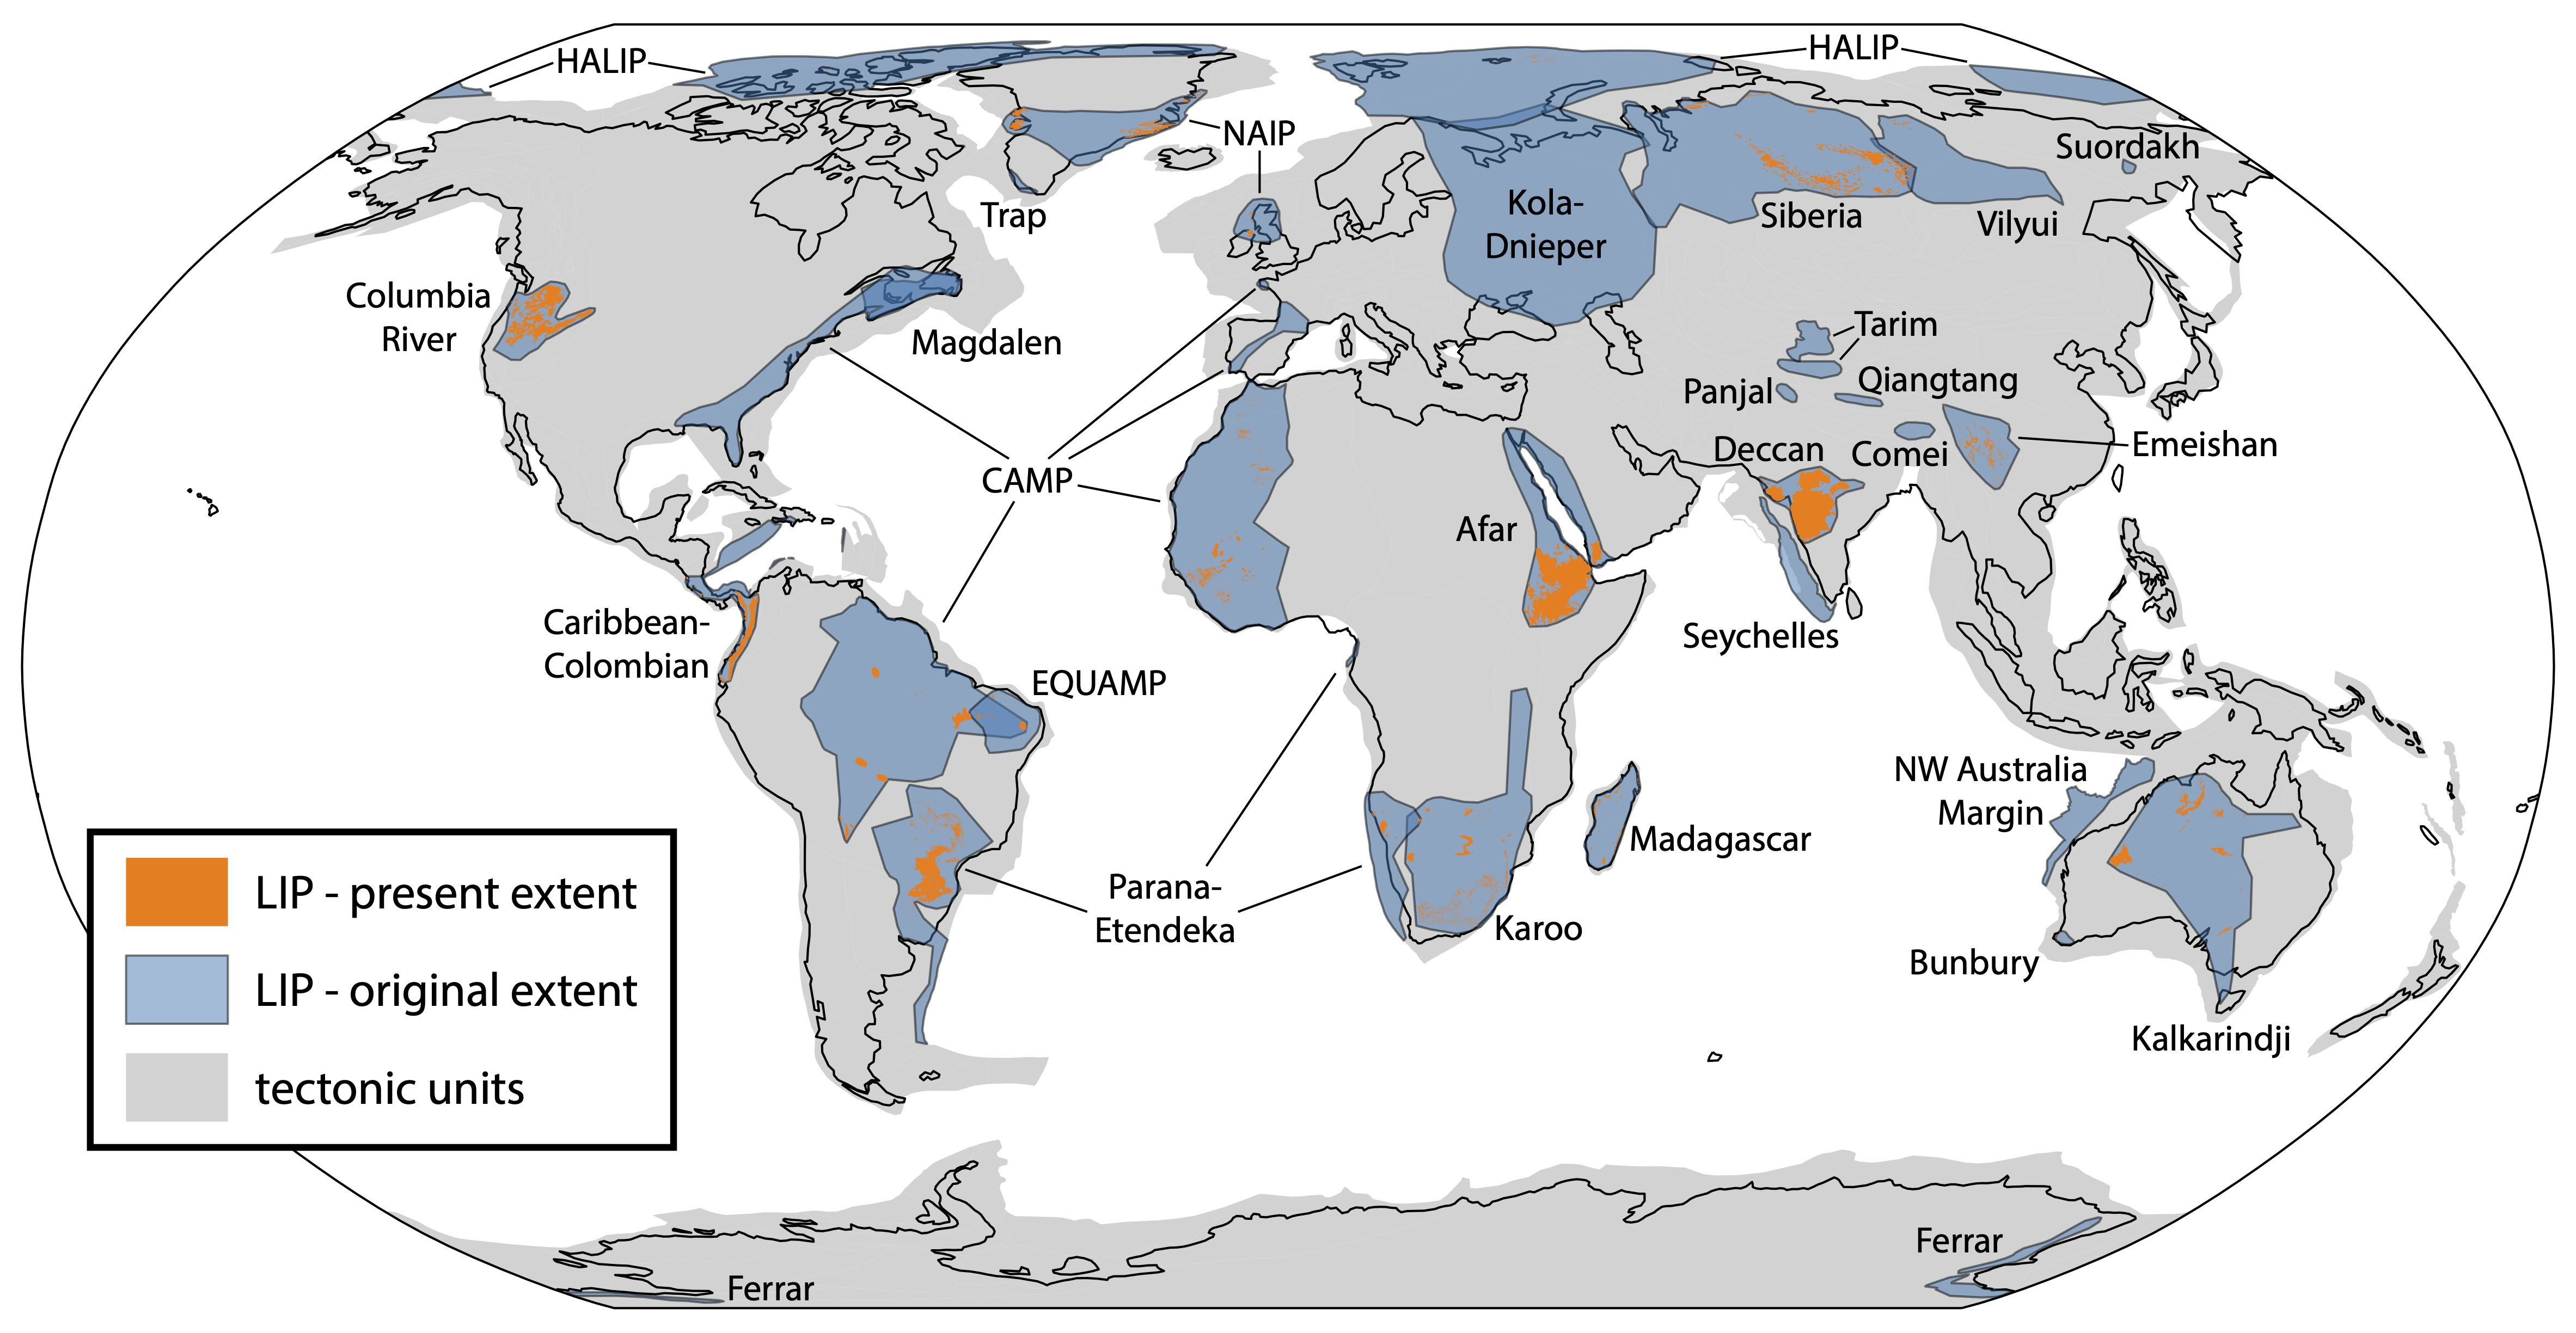
\includegraphics[width=\textwidth]{figures/LIPs/LIP-map.jpg}
	\caption[Map of current surface extent of volcanic lithologies associated with large igneous provinces that erupted between 520~Ma and the present.]{Map of current surface extent of volcanic lithologies associated with LIPs that erupted between 520~Ma and the present, as well as the estimates of the initial LIP surface extent used in the area analysis (modified slightly from \citealp{Ernst2017a} and \citealp{Ernst2019a} to ensure that all currently exposed volcanic lithologies are encapsulated by the initial LIP surface area polygons).}
	\label{fig:LIP-map}
\end{center}
\end{figure}

\begin{table}[h!]
\scriptsize
\caption[Phanerozoic large igneous provinces (and the Franklin).]{Phanerozoic large igneous provinces (and the Franklin).}
\resizebox{0.9\textwidth}{!}{
\begin{tabular}{lc>{\raggedright}p{4cm}cc>{\raggedright}p{4cm}ccl}
\toprule
\textbf{name} & \textbf{age} & \textbf{age ref.} & \textbf{original$^{1}$} & \textbf{present$^{2}$} & \textbf{present area ref.} & \textbf{present/$^{3}$} & \textbf{half-life}$^{4}$ & \textbf{buried?} \\
 & \textbf{(Ma)} & & \textbf{area} & \textbf{area} & & \textbf{original} & \textbf{(Myr)} & \\
 & & & \textbf{(Mm$^{2}$)} & \textbf{(Mm$^{2}$)} & & & & \\
\midrule
Columbia River & 16 & \citet{Kasbohm2018a} & 0.68 & 0.38 & \citet{Buchan2004a} & 0.56 & 19.2 & no \\
 & & & & & & & & \\
Afar & 30 & \citet{Courtillot2003a} & 2.05 & 0.63 & \citet{Coffin2006a} & 0.31 & 17.7 & partial \\
 & & & & & & & & \\
NAIP & 62 & \citet{Larsen2015a} & 1.07 & 0.29 & \citet{Buchan2004a, Coffin2006a} & 0.27 & 33.0 & partial \\
 & & & & & & & & \\
Deccan & 66 & \citet{Schoene2014a} & 0.83 & 0.56 & \citet{Coffin2006a} & 0.68 & 116.6 & no \\
 & & & & & & & & \\
Seychelles & 66 & \citet{Schoene2014a} & 0.46 & 0.00 & \citet{Coffin2006a} & 0.00 & 0.0 & yes \\
 & & & & & & & & \\
Madagascar & 90 & \citet{Cucciniello2010a} & 0.63 & 0.03 & \citet{Coffin2006a} & 0.05 & 20.8 & no \\
 & & & & & & & & \\
Caribbean-Colombian & 94 & \citet{Loewen2013a} & 0.71 & 0.13 & \citet{Coffin2006a} & 0.18 & 37.6 & no \\
 & & & & & & & & \\
HALIP & 95 & \citet{Kingsbury2018a} & 3.60 & 0.15 & \citet{Hartmann2012a} & 0.04 & 20.7 & no \\
 & & & & & & & & \\
EQUAMP & 131 & \citet{Hollanda2016a} & 0.66 & 0.01 & \citet{Hollanda2016a} & 0.01 & 20.5 & no \\
 & & & & & & & & \\
Comei & 132 & \citet{Zhu2009a} & 0.11 & - & - & - & - & no \\
 & & & & & & & & \\
Bunbury & 132 & \citet{Zhu2009a} & 0.03 & 0.00 & \citet{Thorne2014a} & 0.05 & 30.9 & no \\
 & & & & & & & & \\
Parana-Etendeka & 135 & \citet{Florisbal2014a, Almeida2018a} & 3.12 & 0.40 & \citet{Coffin2006a} & 0.13 & 45.7 & partial \\
 & & & & & & & & \\
Trap & 140 & \citet{Ernst2001a} & 0.03 & 0.00 & \citet{Ernst2001a} & 0.00 & 0.0 & no \\
 & & & & & & & & \\
NW Australia Margin & 160 & \citet{Pirajno2012a} & 0.62 & 0.00 & \citet{Coffin2006a} & 0.00 & 0.0 & yes \\
 & & & & & & & & \\
Karoo & 183 & \citet{Burgess2015a} & 3.21 & 0.15 & de Kock compilation$^{5}$ & 0.05 & 41.3 & no \\
 & & & & & & & & \\
Ferrar & 183 & \citet{Burgess2015a} & 0.18 & - & - & - & - & no \\
 & & & & & & & & \\
CAMP & 201 & \citet{Blackburn2013a} & 11.46 & 0.23 & Marzoli and Parisio compilation$^{6}$ & 0.02 & 35.7 & partial \\
 & & & & & & & & \\
Siberia & 252 & \citet{Burgess2015b} & 3.46 & 0.47 & \citet{Coffin2006a} & 0.14 & 87.5 & no \\
 & & & & & & & & \\
Emeishan & 259 & \citet{Zhou2002a} & 0.71 & 0.06 & \citet{Coffin2006a} & 0.09 & 72.9 & no \\
 & & & & & & & & \\
Panjal-Qiangtang & 283 & \citet{Zhai2013a} & 0.11 & - & - & - & - & no \\
 & & & & & & & & \\
Tarim & 290 & \citet{Xu2014a} & 0.35 & - & - & - & - & no \\
 & & & & & & & & \\
Magdalen & 360 & \citet{Murphy1999a} & 0.42 & - & - & - & - & no \\
 & & & & & & & & \\
Vilyui & 374 & \citet{Ricci2013a} & 1.14 & - & - & - & - & no \\
 & & & & & & & & \\
Kola-Dnieper & 380 & \citet{Arzamastsev2014a} & 5.90 & - & - & - & - & no \\
 & & & & & & & & \\
Suordakh & 450 & \citet{Khudoley2013a} & 0.02 & - & - & - & - & no \\
 & & & & & & & & \\
Kalkarindji & 511 & \citet{Jourdan2014a} & 3.54 & 0.17 & \citet{Thorne2014a} & 0.05 & 116.3 & no \\
 & & & & & & & & \\
Franklin & 720 & \citet{Denyszyn2009a} & 2.62 & 0.04 & \citet{Buchan2004a} & 0.02 & 121.8 & no \\
\bottomrule
\end{tabular}
}
\begin{tablenotes}[para,flushleft]
\vspace{0.15cm}
$^{1}$obtained via calculating the area of the continental portions of polygons within the LIP original surface extent compilation of \citet{Ernst2017a} and \citet{Ernst2019a}, shown as blue polygons in Fig. \ref{fig:LIP-map}.
\vspace{0.15cm}

$^{2}$obtained via calculating the area of polygons from the noted reference of presently-exposed volcanics associated with LIPs, shown as orange polygons in Fig. \ref{fig:LIP-map}.
\vspace{0.15cm}

$^{3}$present area / original area
\vspace{0.15cm}

$^{4}$assuming exponential decay with form $N(t) = 2^{t/t_{1/2}}$.
\vspace{0.15cm}

$^{5}$from ArcGIS compilation produced by M. de Kock for the LIPs Reconstruction Project \citep{Ernst2013a}.
\vspace{0.15cm}

$^{6}$from ArcGIS compilation produced by A. Marzoli and L. Parisio for the LIPs Reconstruction Project \citep{Ernst2013a}.
\end{tablenotes}
\label{tab:LIPs}
\end{table}

Outlines of the original surface extent of continental LIPs through the Phanerozoic (Fig. \ref{fig:LIP-map}) were slightly modified (to ensure that all currently exposed volcanic lithologies are encapsulated by the initial LIP area polygons) from the compilation of \citet{Ernst2017a} and \citet{Ernst2019a}, and emplacement ages were taken from the literature (Table \ref{tab:LIPs}). The LIP original surface extent compilation seeks to reconstruct the original surface extent of LIPs with the caveat that there can be significant uncertainty with doing so, particularly for older more deeply eroded LIPs. These polygons encapsulate all of the preserved rocks associated with a given LIP, including dikes, sills, and layered intrusions, in addition to subaerial volcanics (Fig. \ref{fig:LIP-map}). For some LIPs, this approach may lead to an over-estimate of original surface extent, given that subsurface intrusions could extend over a broader area than the surface volcanics. The polygons also assume complete surface coverage between wide-spread remnants, creating further potential for these original extent outlines to be over-estimates. These original extent outlines could also under-estimate the surface area for some LIPs where flows have been eroded and feeder dikes are not exposed or poorly documented. However, despite these uncertainties, this approach likely provides the best estimates available of original surface extent for ancient LIPs. The extents of presently-exposed volcanics associated with LIPs that were used for present-day area estimates (Fig. \ref{fig:LIP-map}) and the sources that went into the construction of the original extent polygons by \citet{Ernst2017a} and \citet{Ernst2019a} were taken from a number of resources including the PLATES compilation \citep{Coffin2006a} and more recent compilation efforts associated with the LIPs Reconstruction Project (\citealp{Ernst2013a}; Table \ref{tab:LIPs}).

\begin{figure}[h!]
\begin{center}
	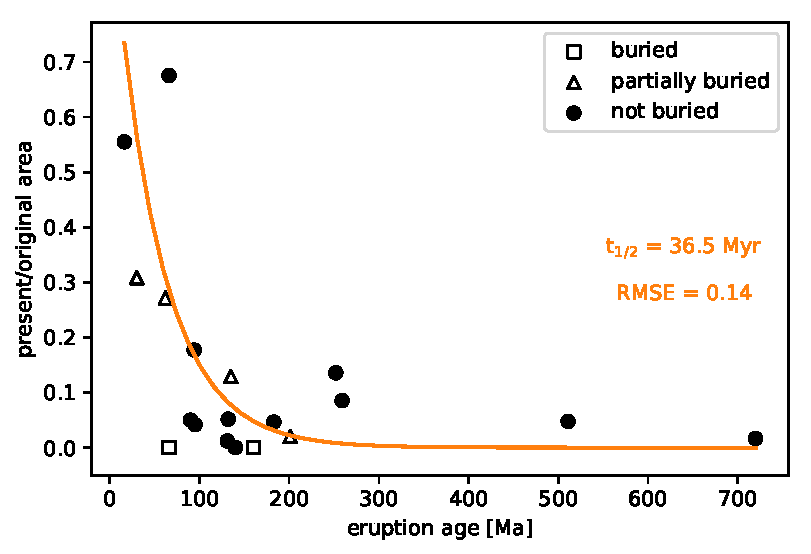
\includegraphics[width=0.6\textwidth]{figures/LIPs/LIP-preservation.pdf}
	\caption[Large igneous province erosion through time.]{LIP erosion through time. The ratio of estimates of the present-day surface area to that of the original surface area are shown for 19 basaltic LIPs. An exponential fit is made to the 13 basaltic LIPs that are interpreted to not have been buried after emplacement (Table \ref{tab:LIPs}), which yields a half-life of $\sim$36~Myr. RMSE = root mean square error.}
	\label{fig:LIP-preservation}
\end{center}
\end{figure}

After LIPs are emplaced, they progressively erode. In order to account for the associated decrease in area with time, \citet{Godderis2017a} took the approach of fitting an exponential decay function to estimates of the original surface extent and the current surface extent of 5 LIPs. They used the resulting exponential decay constants to develop a first-order parameterization of changing LIP area through time. We extend this approach to 19 basaltic LIPs for which there are estimates of the original surface extent of the province and the current surface extent of rocks associated with the province (Fig. \ref{fig:LIP-preservation}). While there are significant uncertainties associated with the area estimates, this compilation suggests that an exponential decay function is an appropriate first-order representation of the progressive reduction in LIP area (Fig. \ref{fig:LIP-preservation}). The best-fit exponential function results in a LIP area half-life of 29~Myr. However, since we explicitly account for LIP burial separately in our area analysis (see below), we exclude from our estimation of a representative LIP area half-life the 6 of 19 LIPs which are inferred to have been partially or completely buried. This latter approach yields a slightly longer best-fit half-life of 36~Myr (Fig. \ref{fig:LIP-preservation}). Although the exponential fit to the 13 unburied LIPs is good (i.e. it yields a low root mean square error of 0.14), if each LIP is fit individually with an exponential decay function, there is variability in the estimated half-lives from $\sim$20~Myr up to $\sim$120~Myr for the Deccan Traps (Table \ref{tab:LIPs}). In the analysis of LIP area through time, we implement decay scenarios informed by these results: the `t$_{1/2}$ = 36~Myr' scenario uses the best-fit half-life of 36~Myr, while the `t$_{1/2}$ = 120~Myr' scenario uses the slower decay. Given that the post-emplacement weathering and erosional history of each LIP should be dependent on the tectonic and climatic setting that each LIP experiences during and after emplacement, this approach is simplistic, but it provides a framework for analysis. The LIP reconstructions used in this study also include pre-Phanerozoic LIPs. However, given the imposed exponential decay since emplacement, the inclusion of these LIPs does not significantly influence the calculated LIP areas through the Phanerozoic, which is the focus of this analysis.

Of the tectonic factors that could alter exposed LIP area, the most consequential is near-immediate burial by sediment of LIP volcanics that are co-located with a rift basin. There are numerous examples in the record where there is partial or complete burial of a LIP associated with rifting and thermal subsidence (Table \ref{tab:LIPs}). For example, the Afar LIP is both associated with the Ethiopian Traps which form plateau flood basalts as well as successful rifting in the region of the Red Sea that has resulted in burial (Fig. \ref{fig:LIP-map}). To account for the rapid decrease in exposed surface area that would result from burial by sediments in a rift basin, we impose two different burial scenarios for LIPs that are co-located with rifting. The `50\% burial' scenario imposes instantaneous burial of 50$\%$ of the LIP area while the `100\% burial' imposes instantaneous burial of the entire LIP as an end-member scenario. A limitation of our treatment of LIPs that are co-located with rifting is that we `bury' all of these LIPs instantly at the time of emplacement and to the same degree when in fact the degree and timing of burial of these LIPs may vary substantially. The LIP area analysis uses all of the available combinations of the distinct decay and burial scenarios described above.

Our LIP reconstruction differs from that of \citet{Johansson2018a}. In contrast to the decay and decay+burial scenarios implemented on estimates of original LIP extent in this study, \citet{Johansson2018a} uses a static extent for each LIP throughout the reconstruction. In their analysis, some of the polygons correspond to the present-day surface extent and some represent the original extent that includes currently buried portions of the LIP. An example of this treatment is the Keweenawan Midcontinent Rift for which the implemented extent in \citet{Johansson2018a} is from geophysical data that largely corresponds to buried subsurface exposures.

The original surface extent LIP polygons were assigned a plate ID corresponding to a tectonic unit on Earth using the polygons of \citet{Torsvik2016a} for the Phanerozoic. The LIP polygons and tectonic units were reconstructed from 520~Ma to the present (e.g. Fig. \ref{fig:reconstruction-snapshots}) utilizing the paleogeographic model of \citet{Torsvik2016a} in the spin axis reference frame (anchor plate ID of 1). This paleogeographic model was updated to include revisions to Ordovician Laurentia \citep{Swanson-Hysell2017a} and Paleozoic Asia \citep{Domeier2018a}. Reconstructions and area calculations within latitude bands utilized the pyGPlates function library and custom Python scripts. The total LIP area and the LIP area reconstructed within the tropical rain belt were calculated for the various decay and burial scenarios at a resolution of 5~Myr (Fig. \ref{fig:LIP-areas}B and C). All the data and code necessary to reproduce the analyses and figures presented in this study can be downloaded from GitHub (\url{https://github.com/Swanson-Hysell-Group/2020_large_igneous_provinces}) or Zenodo (\url{https://doi.org/10.5281/zenodo.3981262}).

\begin{figure}[h!]
\begin{center}
	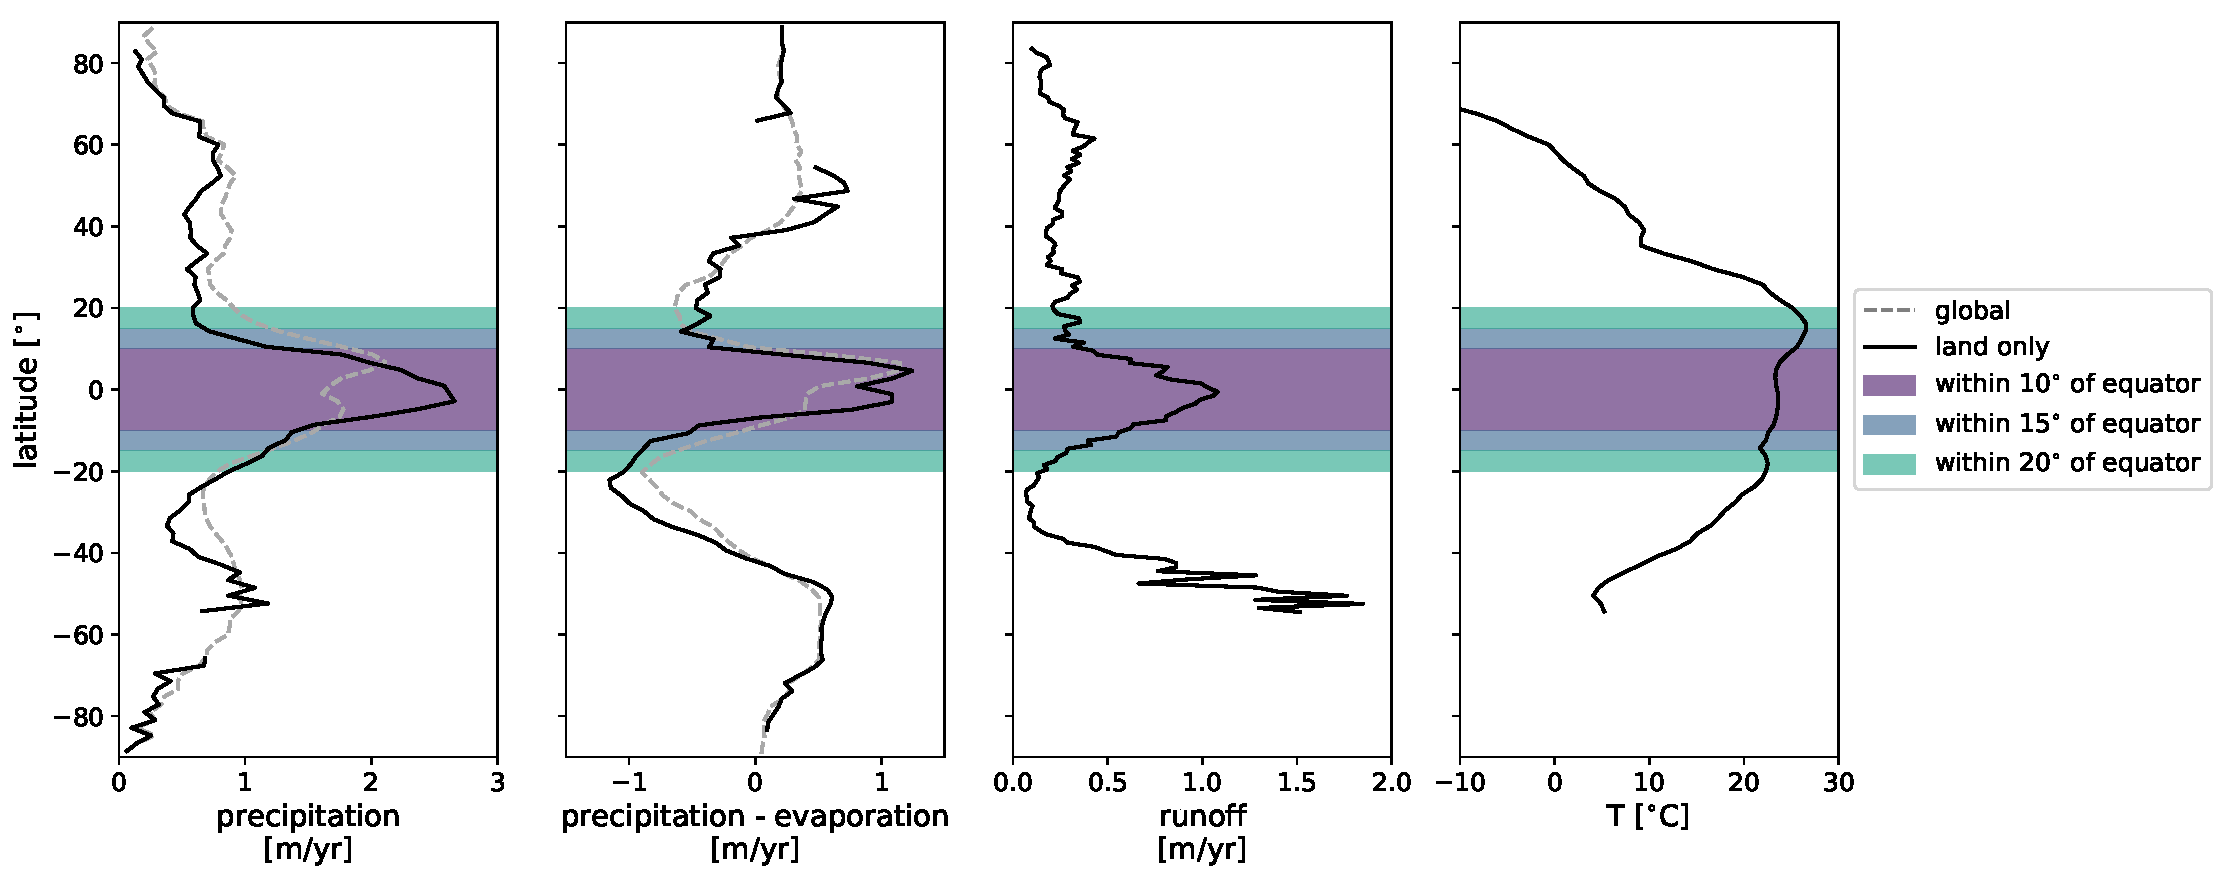
\includegraphics[width=\textwidth]{figures/LIPs/climatology.pdf}
	\caption[Zonally averaged modern climatological data used to define the tropical rain belt.]{Zonally averaged modern climatological data used to define the tropical rain belt. The global precipitation \citep{Kalnay1996a} and precipitation minus evaporation \citep{Trenberth2011a} data include land and ocean pixels, global temperature data \citep{Kalnay1996a} are from land only, and runoff data \citep{Fekete1999a} are from land only excluding Antarctica. The peak in runoff $\sim$-50\degrees is due to anomalously high orographically-induced runoff in the southern Andes, which represents almost all of the land in that latitude belt. Temperature data for Antarctica are off scale. Precipitation, precipitation minus evaporation, and runoff all increase sharply between $\pm$10\degrees and $\pm$15\degrees.}
	\label{fig:climatology}
\end{center}
\end{figure}

\begin{table}[h!]
\scriptsize
\caption[Statistics of correlation between large igneous province area and ice extent.]{Statistics of correlation between large igneous province area and ice extent.}
\resizebox{\textwidth}{!}{
\begin{tabular}{>{\raggedright}p{2.5cm}|cccc|cccc|cccc|cccc}
\toprule
\textbf{} & \multicolumn{4}{c|}{\textbf{within tropics $\pm$15\degrees}} & \multicolumn{4}{c|}{\textbf{total}$^{5}$} & \multicolumn{4}{c|}{\textbf{within tropics $\pm$10\degrees}} & \multicolumn{4}{c}{\textbf{within tropics $\pm$20\degrees}} \\
&&&&&&&&&&&&&&&& \\
\textbf{} & \multicolumn{2}{c}{\textbf{correlation}$^{1}$} & \multicolumn{2}{c|}{\textbf{\% overlap}$^{2}$} & \multicolumn{2}{c}{\textbf{correlation}} & \multicolumn{2}{c|}{\textbf{\% overlap}} & \multicolumn{2}{c}{\textbf{correlation}} & \multicolumn{2}{c|}{\textbf{\% overlap}} & \multicolumn{2}{c}{\textbf{correlation}} & \multicolumn{2}{c}{\textbf{\% overlap}} \\
\textbf{scenario} & \textbf{val.}$^{3}$ & \textbf{p-val.}$^{4}$ & \textbf{val.} & \textbf{p-val.} & \textbf{val.} & \textbf{p-val.} & \textbf{val.} & \textbf{p-val.} & \textbf{val.} & \textbf{p-val.} & \textbf{val.} & \textbf{p-val.} & \textbf{val.} & \textbf{p-val.} & \textbf{val.} & \textbf{p-val.} \\
\midrule
t$_{1/2}$ = 36~Myr & -0.19 & 0.81 & 13 & 0.94 & -0.26 & 0.85 & 30 & 0.95 & -0.22 & 0.86 & 13 & 0.95 & -0.17 & 0.77 & 9 & 0.96 \\
&&&&&&&&&&&&&&&& \\
t$_{1/2}$ = 36~Myr + 50\% burial & -0.14 & 0.73 & 22 & 0.85 & -0.25 & 0.84 & 52 & 0.97 & -0.17 & 0.79 & 9 & 0.90 & -0.10 & 0.67 & 26 & 0.86 \\
&&&&&&&&&&&&&&&& \\
t$_{1/2}$ = 36~Myr + 100\% burial & -0.02 & 0.45 & 22 & 0.65 & -0.14 & 0.74 & 65 & 0.94 & -0.08 & 0.54 & 9 & 0.76 & 0.04 & 0.37 & 22 & 0.65 \\
&&&&&&&&&&&&&&&& \\
t$_{1/2}$ = 120~Myr + 100\% burial & 0.10 & 0.32 & 35 & 0.72 & 0.00 & 0.51 & 100 & 1.00 & 0.02 & 0.40 & 26 & 0.77 & 0.19 & 0.24 & 48 & 0.66 \\
\bottomrule
\end{tabular}
}
\begin{tablenotes}[para,flushleft]
\vspace{0.15cm}
$^{1}$Pearson correlation coefficient between LIP area and the actual ice extent record.
\vspace{0.15cm}

$^{2}$\% of time when both LIP area is \textgreater30\% of the maximum and ice extent is \textgreater10\degrees from the poles.
\vspace{0.15cm}

$^{3}$`val.' refers to the computed correlation coefficient/\% overlap between LIP area and the actual ice extent record.
\vspace{0.15cm}

$^{4}$`p-val.' refers to the fraction of randomly timed glacial interval simulations that correlate/overlap better with LIP area than the actual ice extent record (i.e. the p-value with respect to the null hypothesis of no correlation/overlap). P-values \textless0.05 indicate that we can reject the null hypothesis at the 95\% confidence level.
\vspace{0.15cm}

$^{5}$all latitudes.
\end{tablenotes}
\label{tab:stats}
\end{table}

The ascent of air near the equator associated with Earth's large-scale Hadley circulation promotes precipitation and leads to a low-latitude band of high rainfall known as the tropical rain belt. In contrast, the descending branches of the Hadley circulation in the subtropics are associated with aridity \citep{Manabe1969a}. We use 15\degrees~S to 15\degrees~N as a working definition of the tropical rain belt, as these latitudes approximately correspond with a sharp increase in zonal mean precipitation when approaching the equator to values greater than 1.0~m/yr in modern climatalogical data (\citealp{Kalnay1996a}; Fig. \ref{fig:climatology}). Other parameters that could be used to define the tropical rain belt are runoff and precipitation minus evaporation (P--E). When approaching the equator in modern climatological data, zonal mean runoff sharply increases to values above 0.25~m/yr between approximately $\pm$10\degrees and $\pm$15\degrees (\citealp{Fekete1999a}; Fig. \ref{fig:climatology}), and zonal mean P--E sharply increases to values above 0.5~m/yr also between approximately $\pm$10\degrees and $\pm$15\degrees (\citealp{Trenberth2011a}; Fig. \ref{fig:climatology}). While seasonally high precipitation within $\pm$15\degrees of the equator associated with migration of the intertropical convergence zone could be a driver of high chemical weathering, annual mean runoff is often the value that is used within parameterizations of chemical weathering (e.g. \citealp{West2012a}). Using runoff or P--E favors a definition of the tropical rain belt that is closer to $\pm$10\degrees rather than $\pm$15\degrees. Therefore, we tested the sensitivity of our results to the assumed width of the tropical rain belt by performing the tropical LIP area calculations with a tropical rain belt width of $\pm$10\degrees. We also calculated the area of LIPs within $\pm$20\degrees of the equator (a width that includes part of the arid subtropics) in order to account for uncertainties in the paleolatitude of LIPs in the paleogeographic model. We find that both of these additional analyses (LIP area calculated within $\pm$10\degrees and $\pm$20\degrees of the equator) yield similar results to those obtained when LIP area is calculated within $\pm$15\degrees of the equator (Table \ref{tab:stats}).

In \citet{Evans2006a}, the reconstructed paleolatitudes of basins with thick, basin-wide evaporite deposition are shown to be consistently in the subtropics throughout the Phanerozoic and the Proterozoic, suggesting that the large-scale atmospheric circulation that gives rise to intense precipitation in the tropical rain belt and an arid subtropical climate is stable through time. However, subsequent work by \citet{Boucot2013a} and \citet{Cao2018a} has interpreted evaporite deposits to have formed at or near the equator at times in the Phanerozoic. While some of this variability could be attributed to waxing/waning of the width of the tropical rain belt as a whole, it is important to note that there can be large deviations in local precipitation from the zonal mean due to factors such as monsoon-related precipitation \citep{Trenberth2000a}, or continentality (i.e. how dispersed or amalgamated the continents are) which can lead to aridity in continental interiors. For instance, much of the Early Cretaceous low-latitude evaporite deposits were formed in basins that were located deep within arid continental interiors at the time of deposition \citep{Boucot2013a, Cao2018a}. In contrast to \citet{Evans2006a}, the compilation of evaporite deposits of \citet{Boucot2013a} contains sedimentary sequences in which the occurrence of evaporitic minerals is limited (e.g. to disseminated gypsum pseudomorphs). Such limited evaporitic mineral precipitation could be attributed to seasonal evaporation that transiently led to saturation states that otherwise would not be expected for that latitude. Nevertheless, a limitation of the LIP analysis described in this study is that it does not account for deviations in local precipitation from the zonal mean (due to the infeasibility of running a highly-resolved global climate model at each time-step in the analysis). However, evaporite deposits, including those in which the occurrence of evaporitic minerals is limited, are distributed bimodally about the equator in the subtropics for the vast majority of the past $\sim$420~Myr \citep{Cao2018a} and overall stability of the large-scale atmospheric circulation is predicted by climate dynamics \citep{Donohoe2017a}. Therefore, the assumption of enhanced precipitation and runoff in the tropics throughout the Phanerozoic is warranted.

\begin{figure}[h!]
\begin{center}
	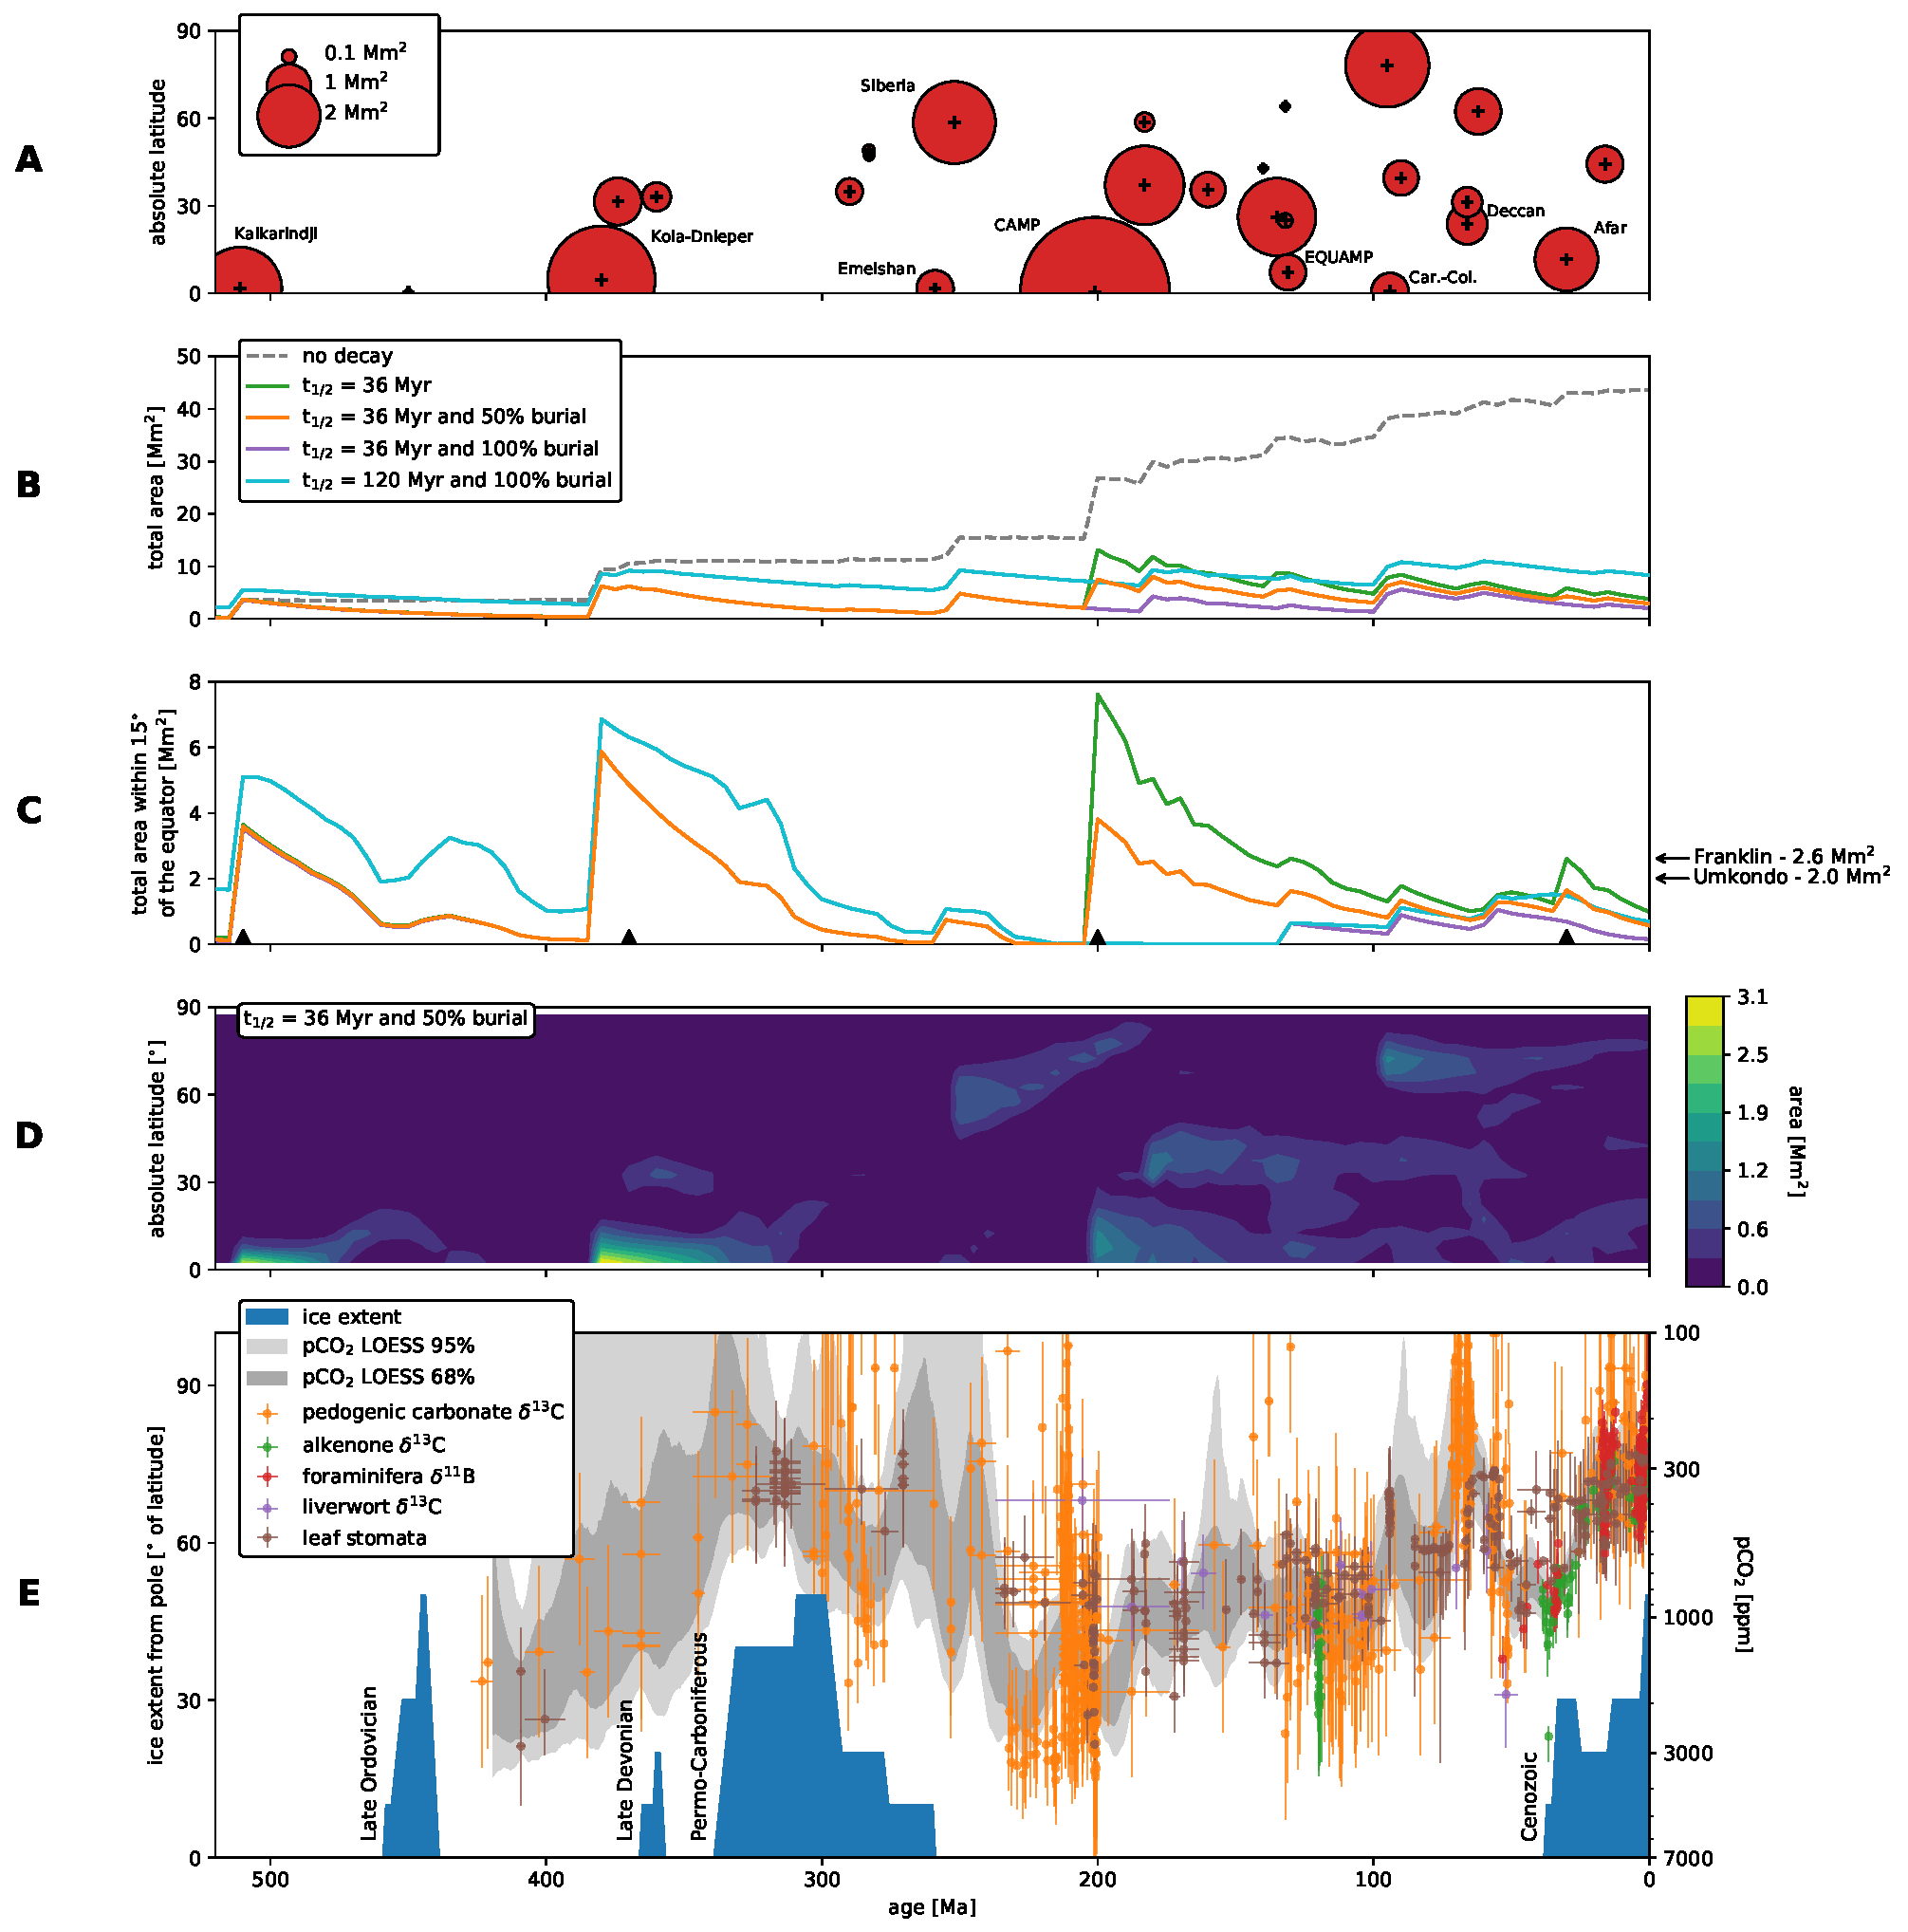
\includegraphics[width=0.8\textwidth]{figures/LIPs/LIP-areas.pdf}
	\caption[Reconstructed large igneous province areas, ice extent, and \pCOtwo proxies.]{\textbf{A)} LIPs included in this analysis. The size of each circle reflects the initial surface area estimate of each LIP. The + indicates the timing and absolute paleolatitude of the centroid of each LIP at the time of emplacement. Car.-Col. = Caribbean-Colombian. \textbf{B)} Total LIP area through time for the different post-emplacent scenarios. Only the `no decay' scenario excludes pre-Phanerozoic LIPs. \textbf{C)} Tropical LIP area through time for the different post-emplacement scenarios. The arrows to the right indicate reconstructed tropical LIP area at the time of emplacement for the ca. 720 and 1109~Ma Franklin and Umkondo LIPs. The triangles show the paleogeographic reconstruction times in Fig. \ref{fig:reconstruction-snapshots}. \textbf{D)} Contour plot showing the latitudinal distribution of LIP area for one of the post-emplacement models. \textbf{E)} Latitudinal extent of land ice away from the poles \citep{Macdonald2019a} and compilation of \pCOtwo proxies \citep{Foster2017a} (\pCOtwo y-axis reversed, and in log-scale). Error bars indicate standardized uncertainties, and grey bands indicate 68 and 95\% confidence intervals for Monte Carlo resampled LOESS fits to the \pCOtwo proxy data \citep{Foster2017a}. Note that there are \pCOtwo proxy estimates \textless100~ppm that are cut off in this plot.}
	\label{fig:LIP-areas}
\end{center}
\end{figure}

To evaluate the relationship between Earth's climate state and total and tropical LIP area, we compared these areas to a compilation of the latitudinal extent of continental ice sheets over the Phanerozoic (\citealp{Macdonald2019a}; Fig. \ref{fig:LIP-areas}E). The goal in doing so is to evaluate the hypothesis that there is a correlation between LIP area in the tropics and Earth's long-term climate state. The land ice record is an imperfect tracker of climate as it is insensitive to changes in temperature during non-glacial intervals, is influenced by additional factors such as the physical geography of the continents during glacial intervals, and is potentially vulnerable to removal from the observable geologic record via erosion and burial. Furthermore, the threshold \pCOtwo for establishing a glacial climate is dependent on ocean circulation and changing solar luminosity (e.g. \citealp{Shevenell2004a, DeConto2008a}). Nevertheless, it forms a physical record of Earth's climate through time and delineates glacial and non-glacial climate states. We take two approaches for comparison between the LIP area reconstructions and the record of ice extent. The first is to calculate the Pearson correlation coefficient between LIP area and the extent of ice away from the pole. The second is to consider the degree of overlap between intervals of high LIP area (defined as LIP area \textgreater30\% of the maximum in a given post-emplacement model) and intervals of glacial climate (defined as ice extent \textgreater10\degrees from the poles). This overlap approach places less emphasis on the specific magnitudes of the peaks in the compiled ice extent and LIP area records.

Another approach would be to compare the LIP area reconstructions to proxy compilations of \pCOtwo (as done by \citealp{Johansson2018a}) instead of the latitudinal extent of continental ice sheets. However, such \pCOtwo proxies are potentially problematic as they can be difficult to calibrate in deep time and can be affected by secondary alteration. Even when stringent quality criteria and the latest understanding of each of the \pCOtwo proxies have been applied to available \pCOtwo records \citep{Foster2017a}, both significant uncertainty in the estimated \pCOtwo for any given data point as well as disagreement between techniques remain (Fig. \ref{fig:LIP-areas}E). For instance, in the Late Triassic ($\sim$240-200~Ma), estimates of \pCOtwo span $\sim$3000~ppm. Even a probabilistic approach to a large \pCOtwo proxy data set can not constrain \pCOtwo at the 95\% confidence level to within a few hundred ppm for any given time interval, especially when we look deeper in time than the Cenozoic (\citealp{Foster2017a}; Fig. \ref{fig:LIP-areas}E). For the pedogenic carbonate \dC proxy, which forms the majority of the pre-Cenozoic data in the compilation of \citet{Foster2017a}, such scatter could result from diagenesis \citep{Michel2016a} and the sensitivity of the \pCOtwo estimates on assumptions regarding soil-respired \COtwo \citep{Montanez2013a}. Nevertheless, despite these shortcomings, the \pCOtwo proxy record is broadly consistent with the ice extent record (Fig. \ref{fig:LIP-areas}E) - \pCOtwo proxy data decreases $\sim$400-310~Ma as the Late Devonian glacial interval occurs and the Permo-Carboniferous glacial interval begins and waxes, \pCOtwo proxy data roughly increases $\sim$310-240~Ma as the Permo-Carboniferous glacial interval wanes and ends, \pCOtwo proxy data broadly remains relatively high $\sim$240-40~Ma when no glacial intervals are robustly documented, and \pCOtwo proxy data roughly decreases $\sim$40-0~Ma as the Cenozoic glacial interval begins. Given these considerations, we thus prefer to use the latitudinal extent of land ice to reflect Earth's overall climate state throughout the Phanerozoic, despite its own limitations.

\section{Results}

\begin{figure}[h!]
\begin{center}
	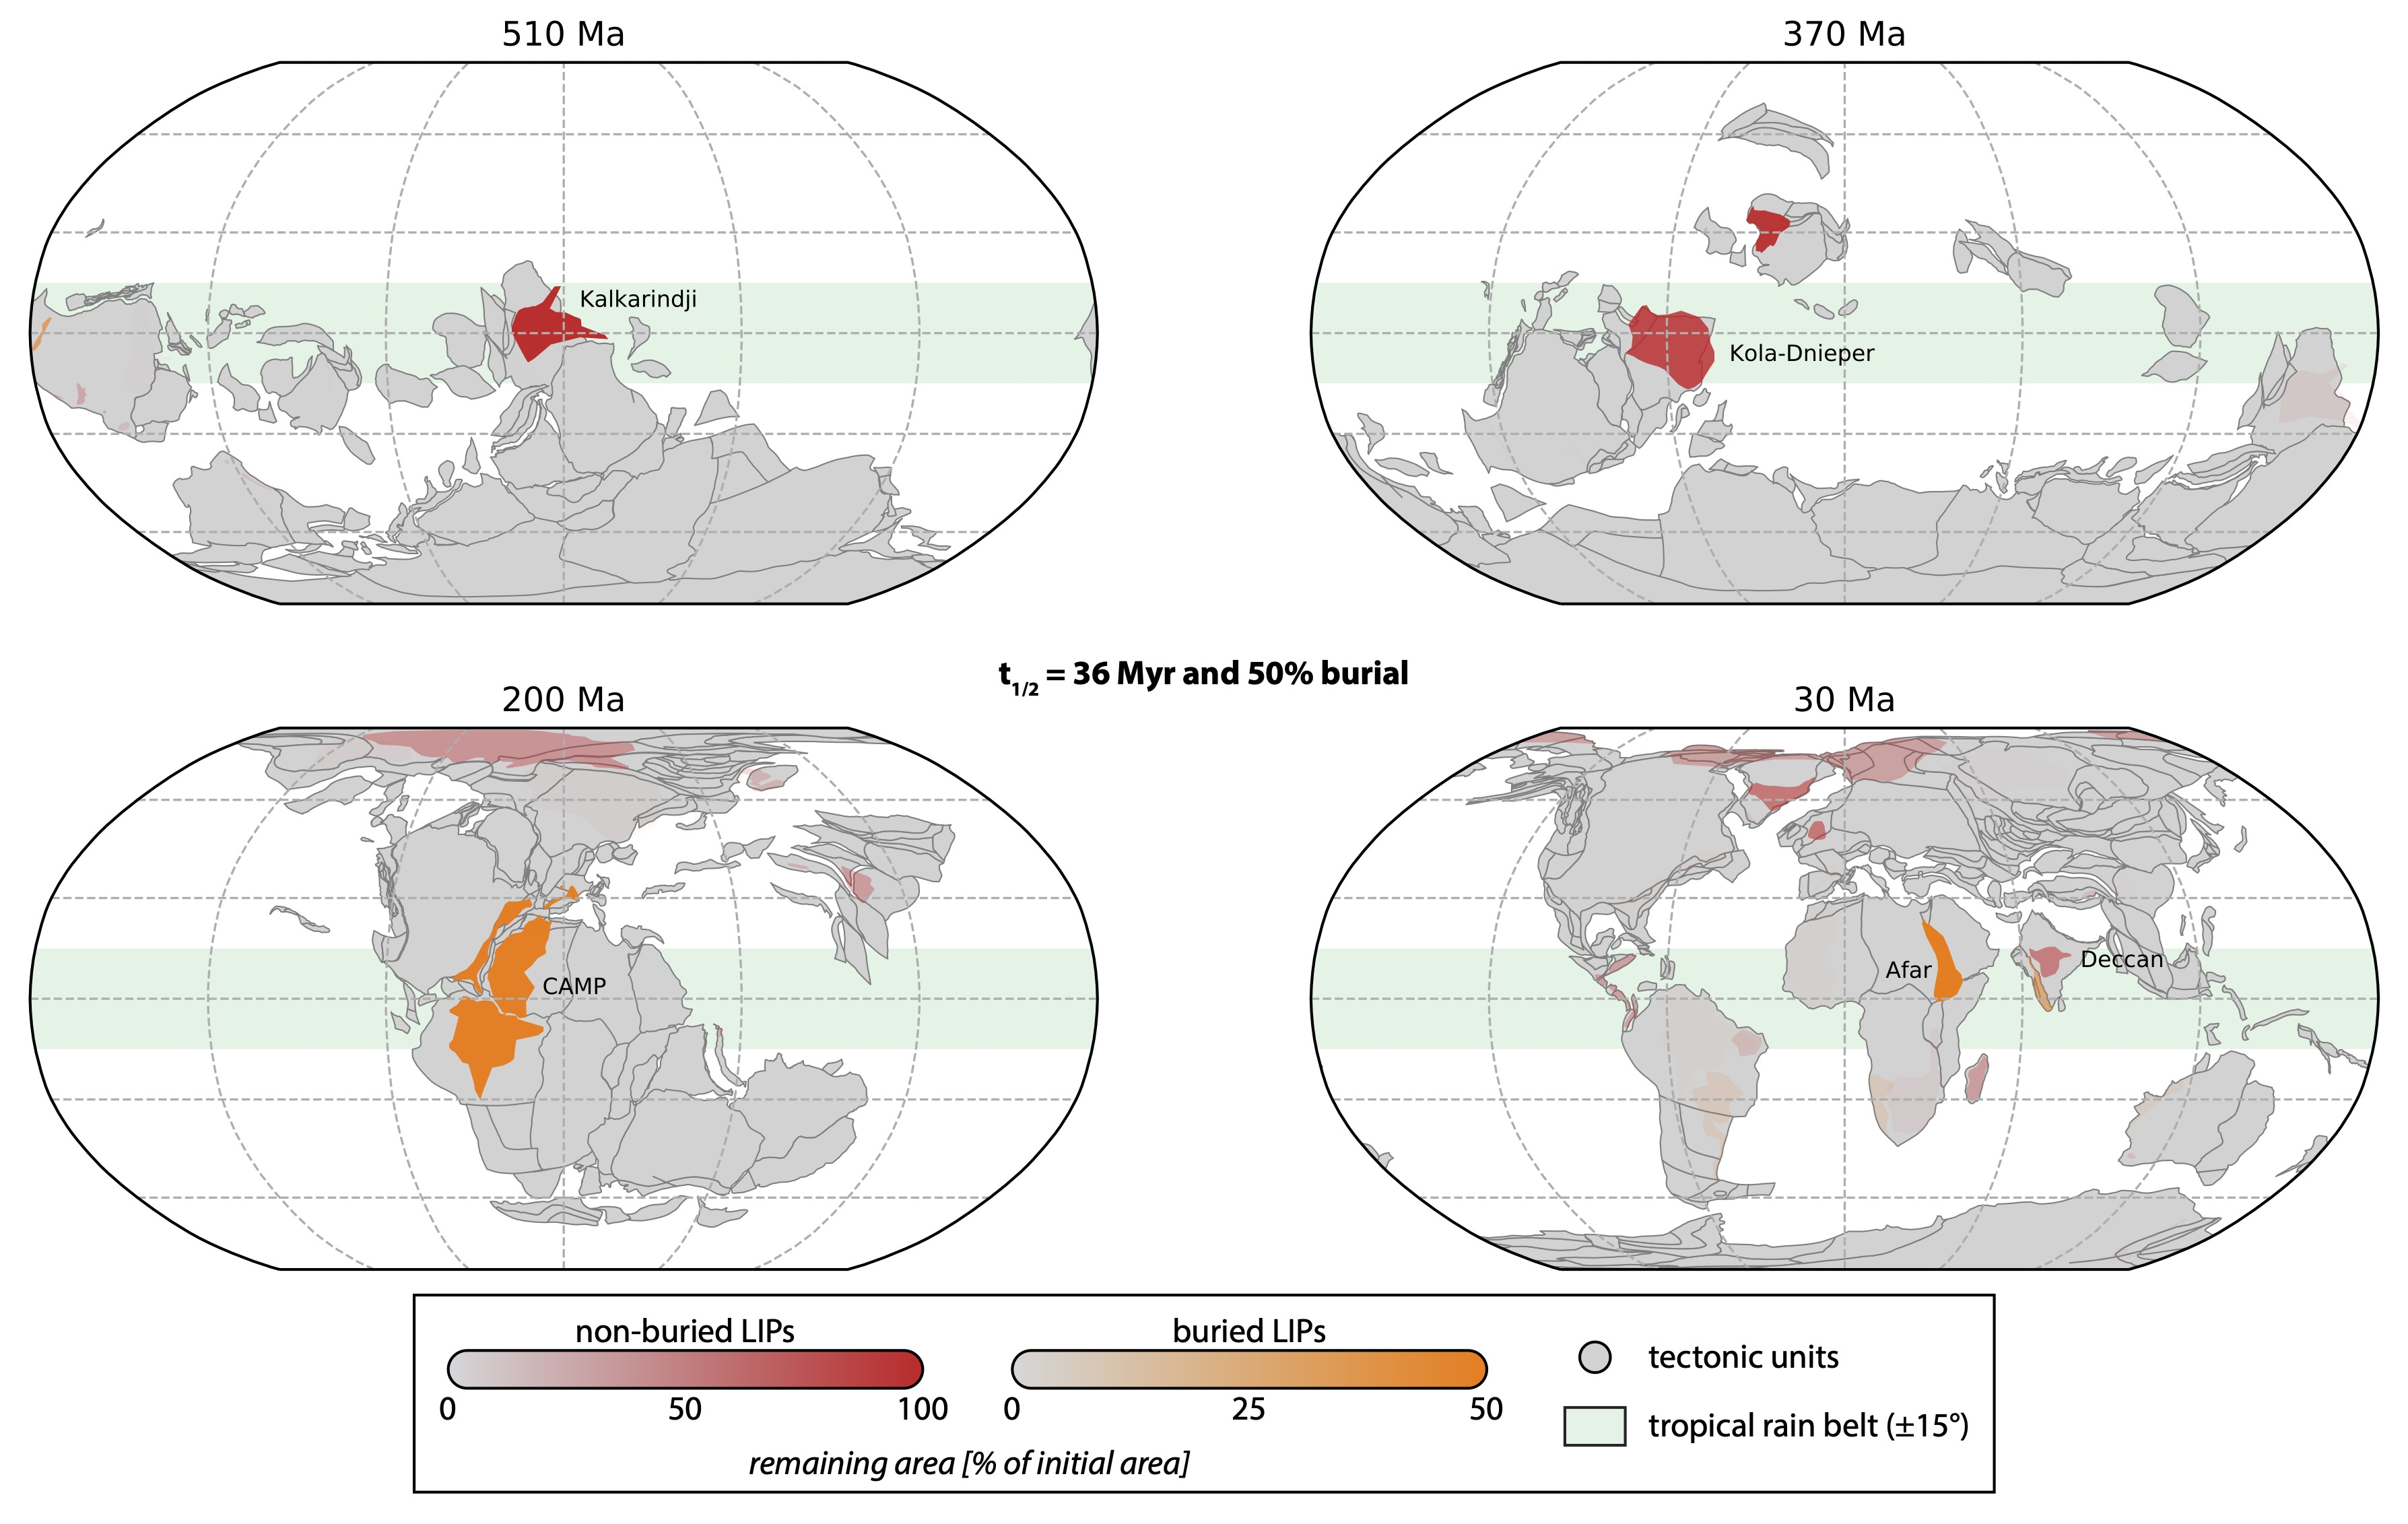
\includegraphics[width=\textwidth]{figures/LIPs/reconstruction-snapshots.jpg}
	\caption[Paleogeographic reconstructions for times that correspond to peaks of large igneous province area in the tropics.]{Paleogeographic reconstructions for times that correspond to peaks of LIP area in the tropics (Fig. \ref{fig:LIP-areas}C). The opacity of LIP polygons indicates their parameterized remaining area at the time of the reconstruction as a percentage of initial LIP area, under the preferred post-emplacement scenario of `t$_{1/2}$ = 36~Myr + 50\% burial'.}
	\label{fig:reconstruction-snapshots}
\end{center}
\end{figure}

In the `t$_{1/2}$ = 36~Myr' scenario, we observe four main peaks in the calculated LIP area within the tropics (Fig. \ref{fig:LIP-areas}C). The first peak ca. 510~Ma is associated with the emplacement of the Kalkarindji LIP, the second peak ca. 380~Ma is associated with the emplacement of the Kola-Dnieper LIP, the third peak ca. 200~Ma is associated with the emplacement of the Central Atlantic Magmatic Province (CAMP), and the fourth peak is associated with both the ca. 30~Ma emplacement of the Afar LIP as well as the earlier drift of the ca. 66~Ma Deccan LIP into the tropics (Figs. \ref{fig:LIP-areas}A and \ref{fig:reconstruction-snapshots}). When we account for burial (`t$_{1/2}$ = 36~Myr + 50\% burial' and `t$_{1/2}$ = 36~Myr + 100\% burial' scenarios), only the latter two of these four peaks are affected -- the ca. 200~Ma peak is attenuated/removed due to the partial/complete burial of the CAMP, and the Cenozoic peak is attenuated due to the partial/complete burial of the Afar LIP. However, after accounting for burial, a minor area of LIPs remain in the tropics from ca. 130~Ma onwards, due to the Equatorial Atlantic Magmatic Province (EQUAMP), Caribbean-Colombian, and Deccan LIPs. Using the longer decay half-life of 120~Myr (the `t$_{1/2}$ = 120~Myr + 100\% burial' scenario) increases the area of LIPs in the tropics at any given time step, and has the effect of extending the duration of each peak.

\begin{figure}[h!]
\begin{center}
	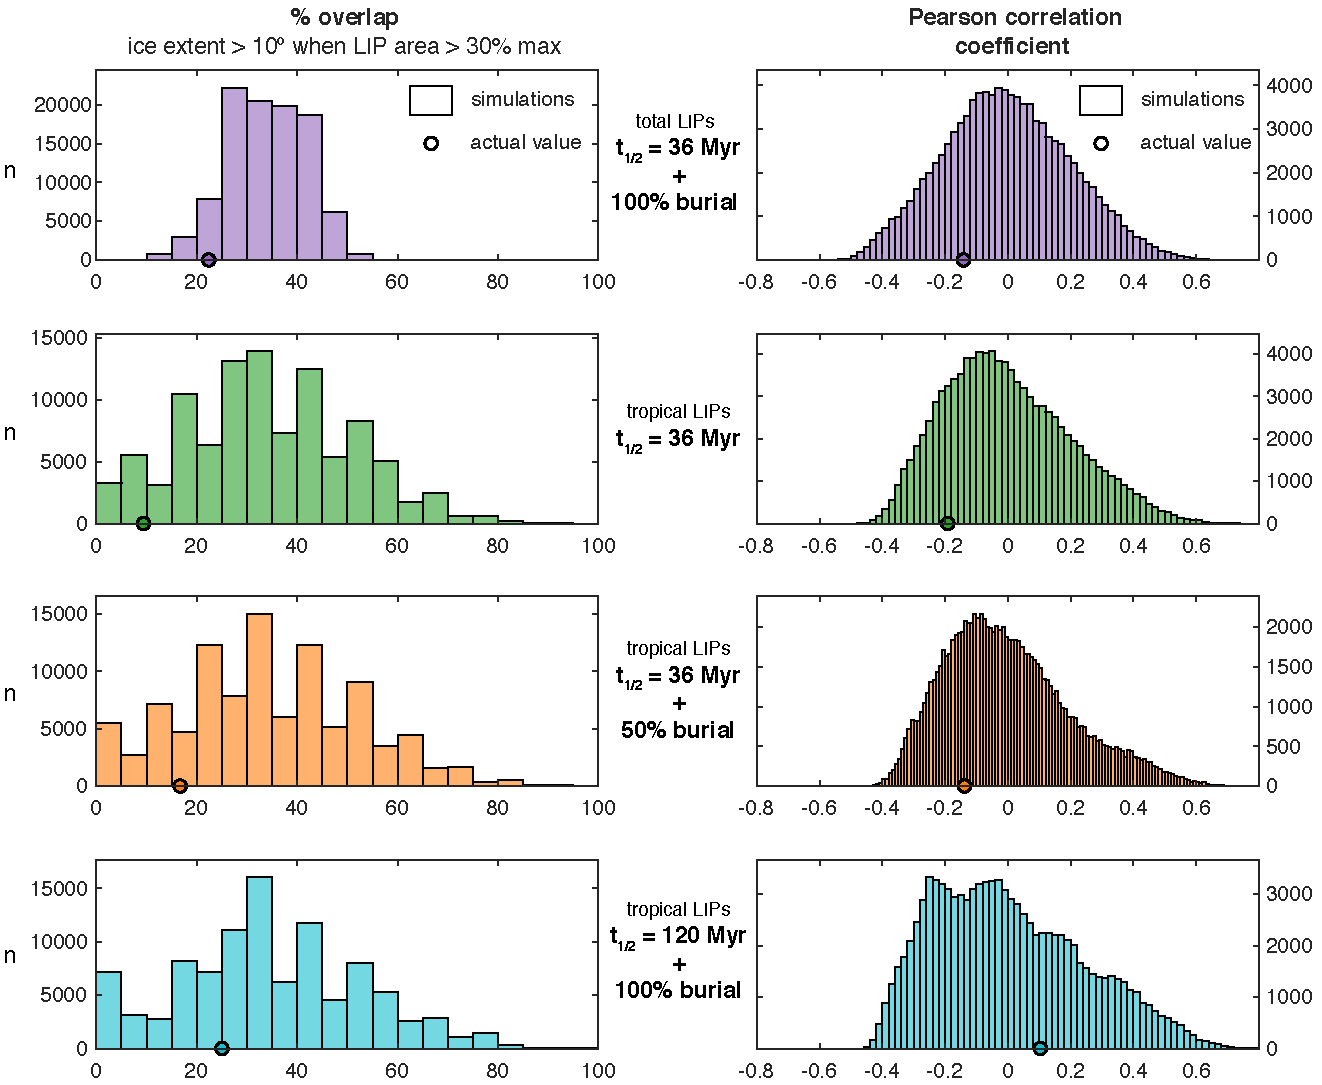
\includegraphics[width=0.85\textwidth]{figures/LIPs/overlap-correlation.pdf}
	\caption[Correlation between large igneous province area and the actual and simulated ice-extent records.]{The \% overlap and Pearson correlation coefficients between LIP area and the actual ice-extent record are shown with circles. These values are compared to histograms that show the range of values that arise when comparing the LIP area record to glacial intervals that have been shifted randomly in time 100,000 times. The fraction of randomly timed glacial interval simulations that correlate/overlap better with LIP area than the actual ice-extent record is the p-value shown in Table \ref{tab:stats}.}
	\label{fig:LIP-correlation}
\end{center}
\end{figure}

The only scenario which results in a non-negative Pearson correlation coefficient (0.10) between LIP area in the tropics ($\pm$15\degrees; Fig. \ref{fig:LIP-areas}C) and the ice extent record (Fig. \ref{fig:LIP-areas}E) is the scenario with the slow decay rate and complete burial of LIPs associated with rifting (the `t$_{1/2}$ = 120~Myr + 100\% burial' scenario; Fig. \ref{fig:LIP-correlation}). All other scenarios (including both total LIP area and tropical LIP area) yield a near zero or weak negative correlation coefficient (Fig. \ref{fig:LIP-correlation}). The weak positive correlation of the `t$_{1/2}$ = 120~Myr + 100\% burial' scenario relative to the other scenarios can be primarily attributed to the complete removal of the CAMP, which was emplaced during an extended interval of ice-free conditions, as well as the effect of the longer decay half-life extending the duration of the earlier two peaks, such that they overlap more with the Late Ordovician and Permo-Carboniferous glacial intervals.

To assess the statistical significance of the correlation implied by the Pearson correlation coefficients (or lack thereof), we applied the approach of \citet{Macdonald2019a} and simulated the four glacial episodes (Fig. \ref{fig:LIP-areas}E) occurring at random times through the past 520~Myr, and recomputed the correlation coefficient and \% overlap between the LIP area in the tropics and the randomly timed glacial intervals for each of these 100,000 simulations (Fig. \ref{fig:LIP-correlation}). This approach accounts for the fact that spurious correlation can arise between auto-correlated data sets such as these, where each value is not independent, but is instead dependent on the previous state of the system. For the `t$_{1/2}$ = 120~Myr + 100\% burial' scenario, 72\% of the randomly timed glacial interval simulations correlate better with LIP area in the tropics than the actual ice extent record. With an associated p-value of 0.72, the null hypothesis that glacial intervals do not correlate to LIP area in the tropics cannot be rejected. Taking this approach, none of the positive or negative correlations that emerge between the LIP area scenarios and the ice extent record are statistically significant (Table \ref{tab:stats}).

\section{Discussion}

In the original models that proposed the `Fire and Ice' hypothesis as an explanation for the onset of the Sturtian `Snowball Earth' glaciation, chemical weathering was modeled as a function of temperature and runoff only \citep{Donnadieu2004a}. However, such an approach neglects the effects of soil shielding and regolith development in low-relief regions. Recent progress on understanding the relationships between landscapes, topography, and chemical weathering reveals that these effects are important \citep{Gabet2009a, Hartmann2014a, Maher2014a, Godderis2017b}. Soil shielding can lead to a transport-limited weathering regime in which the weathering rate of the underlying bedrock becomes insensitive to kinetic and equilibrium factors such as temperature and runoff - factors that would, in the absence of soil shielding, lead to relatively high weathering rates in the tropical rain belt. As a result, more recent modeling of chemical weathering incorporates such processes and highlights the importance of high-relief regions relative to low-relief ones for setting global weatherability \citep{West2012a, Godderis2017b}. LIPs are often emplaced in relatively low-relief areas, and as such, without active uplift, soil shielding from regolith development on these low-relief LIPs could significantly decrease the local weatherability of a LIP and mute its impact on global weatherability (as suggested in \citealp{Kent2013a}). In this way, soil shielding could explain the lack of correlation between tropical LIP area and ice extent (Figs. \ref{fig:LIP-areas} and \ref{fig:LIP-correlation}). In contrast, processes that lead to continued exhumation of mafic lithologies and the creation of steep topography that minimizes soil shielding, particularly in tropical regions, may exert a strong control on global weatherability and long-term climate. This interpretation underlies the hypothesis that arc-continent collisions in the tropics during the Ordovician \citep{Swanson-Hysell2017a} and the Cenozoic \citep{Jagoutz2016a} played a significant role in transitions into glacial climate states at those times - a correlation that appears robust throughout the Phanerozoic \citep{Macdonald2019a}.

A complication with the interpretation of soil shielding and limited weathering of LIPs is the rapid area decay rate (t$_{1/2}$ = 36~Myr) inferred from the comparison of current LIP surface extent to estimated original surface extent (Fig. \ref{fig:LIP-preservation}). A couple considerations are relevant with respect to this analysis: 1) the current surface extent of LIP exposure is reduced in part by volcanics being covered by unconsolidated sediments (i.e. regolith development itself) in a number of the provinces; 2) the current surface extent of LIP exposure may be incomplete and an underestimate for some of the provinces; 3) the initial LIP surface extents are typically poorly constrained and are likely over-estimates which could be resulting in inflated interpreted decay rates; and 4) the relationship between LIP area and volume is poorly constrained. Future efforts that improve the LIP database, such as developing better-constrained estimates of original LIP surface extent, constraining burial and uplift histories, and refining the timing of eruptions associated with LIPs, will improve analyses that consider the LIP record in its entirety, such as that in this contribution.

We have focused this analysis on the Phanerozoic record given that well-constrained paleogeographic models are available for the past $\sim$520~Myr. The approach of seeking to evaluate correlation between LIP area and glaciation is further complicated for Neoproterozoic Snowball Earth events because ice-albedo runaway leads to persistent global glaciation on timescales of tens of millions of years without continued forcing through normal carbon cycle processes until sufficient \COtwo to drive deglaciation builds up in the absence of silicate weathering \citep{Hoffman2017a}. Moreover, cooling past the critical threshold for rapid global glaciation may have occurred on a sub-million year timescale (e.g. \citealp{Macdonald2017a}). Nevertheless, evaluating the hypothesis of tropical LIP area associated with the ca. 720~Ma Franklin LIP increasing global weatherability and contributing to the onset of the Sturtian Snowball Earth is a major motivating driver behind conducting this analysis.

How does the tropical LIP area associated with the Franklin LIP compare to that observed in the Phanerozoic? Using the paleomagnetic pole of \citet{Denyszyn2009a}, we reconstruct the paleolatitude of the Franklin LIP at the time of emplacement, and find that $\sim$99.7\% (or $\sim$2.6~Mm$^{2}$) of the LIP erupted within 15\degrees of the equator. This Franklin LIP tropical area at the time of emplacement is approximately equivalent to the Cenozoic peak, and is smaller than the other Phanerozoic peaks (Fig. \ref{fig:LIP-areas}C). The ca. 1109~Ma Umkondo is another Precambrian LIP that is constrained to have erupted in the tropics, although it is not known to be associated with any glaciation (no glacial deposits are found within the contemporaneous Midcontinent Rift basin; \citealp{Swanson-Hysell2019a}). We reconstruct the paleolatitude of the Umkondo LIP at the time of emplacement using the paleomagnetic pole of \citet{Swanson-Hysell2015b}, and find that effectively all of the LIP (or $\sim$2.0~Mm$^{2}$) erupted within the tropics, an area that is slightly smaller than that estimated for the Franklin LIP (Fig. \ref{fig:LIP-areas}C).

\begin{figure}[h!]
\begin{center}
	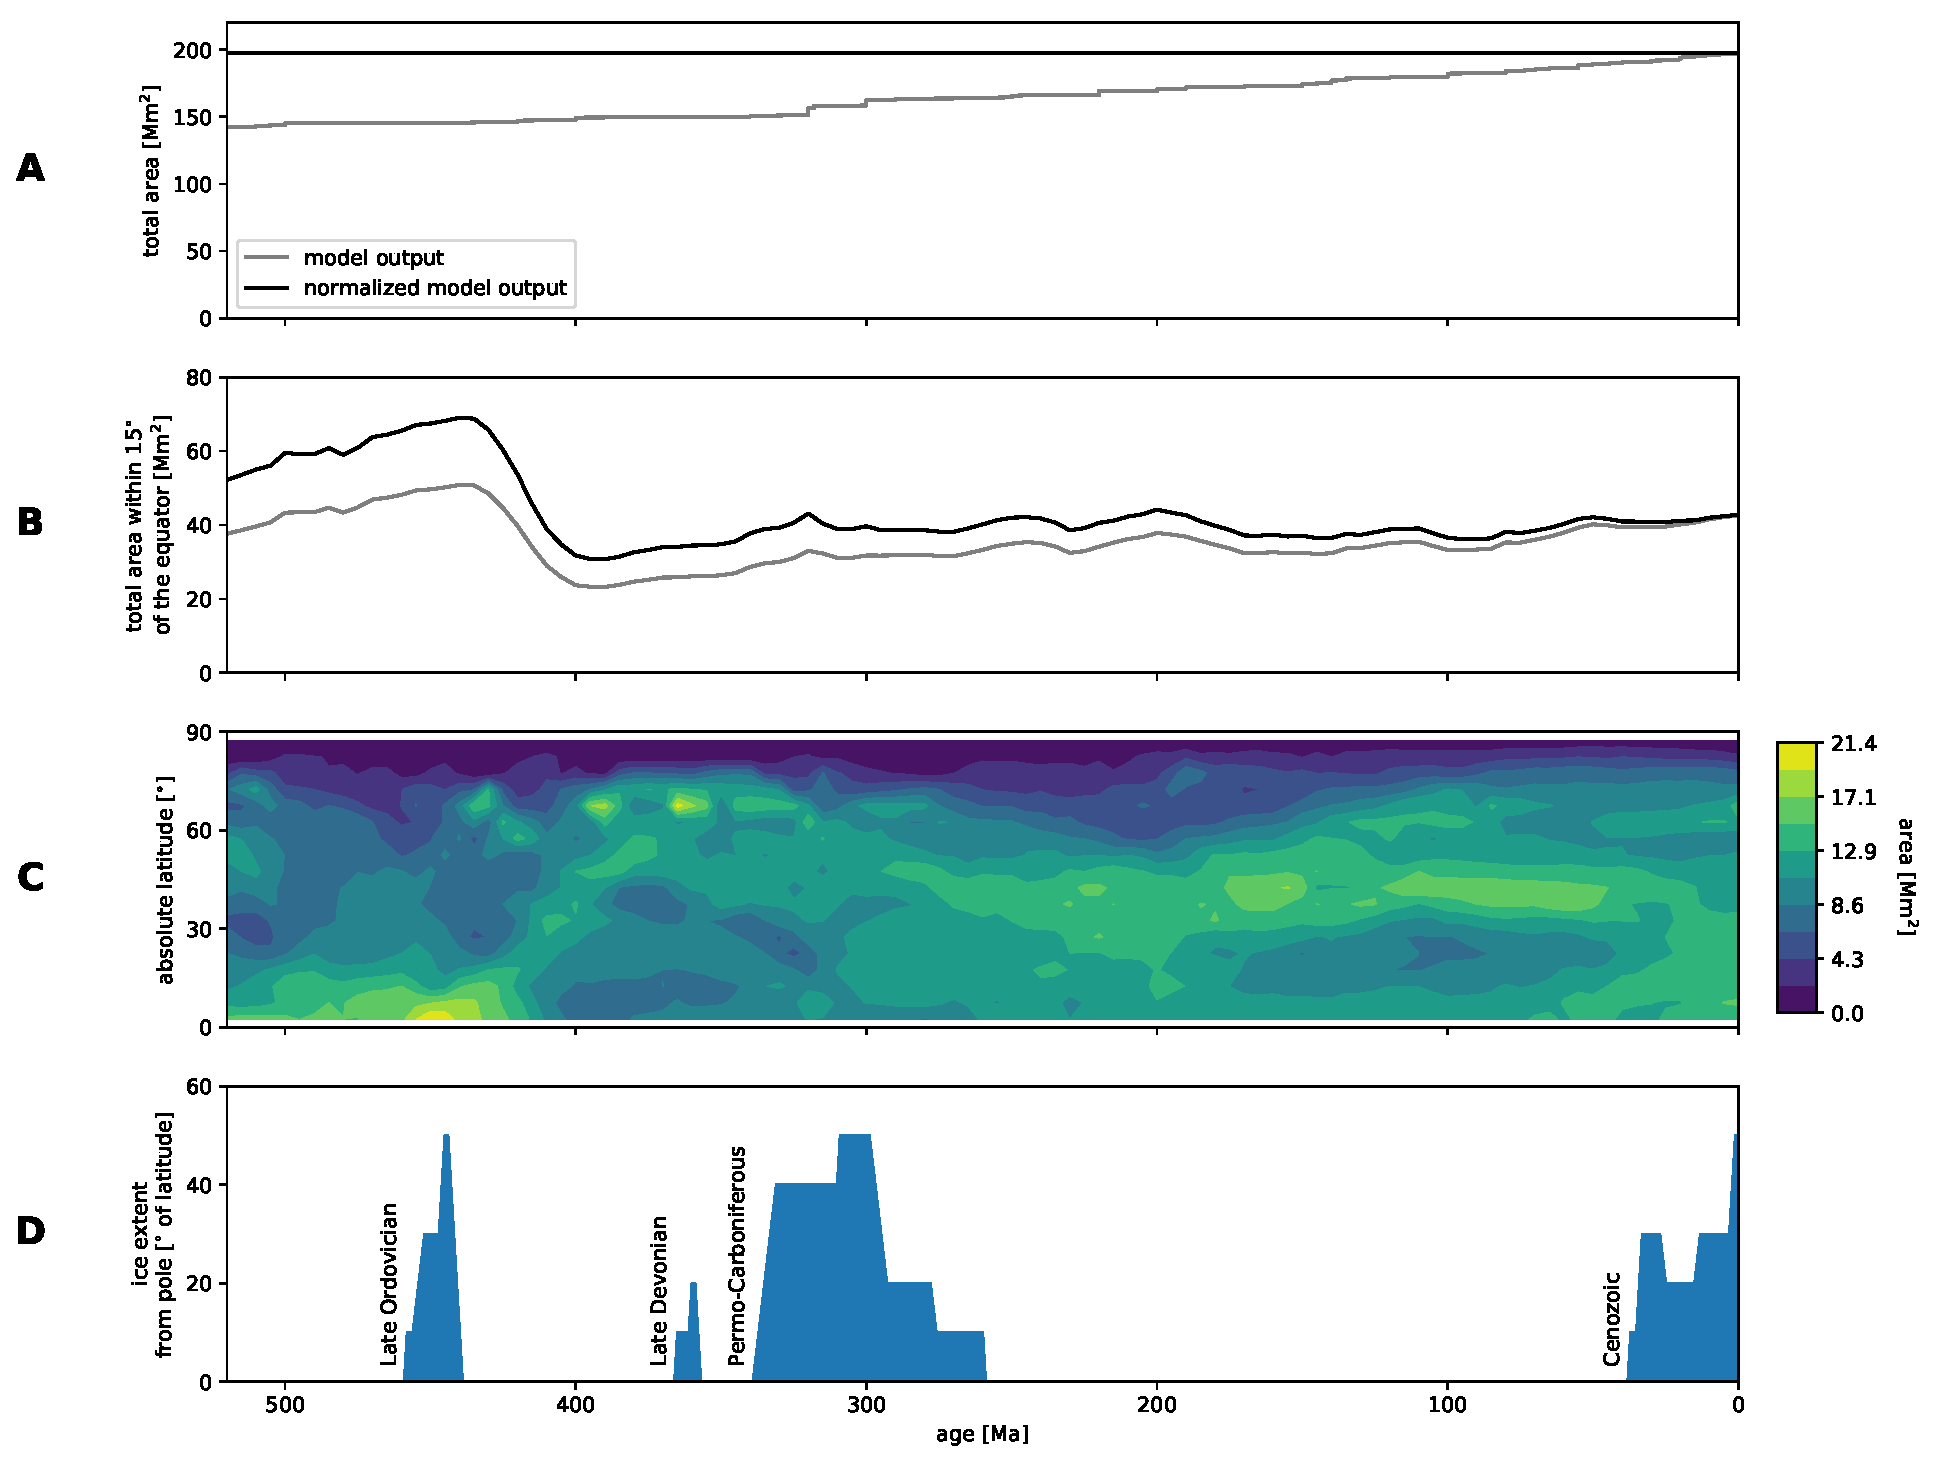
\includegraphics[width=0.9\textwidth]{figures/LIPs/continent-areas.pdf}
	\caption[Reconstructed continental areas.]{\textbf{A)} Total continental area through time. In the paleogeographic model used in this study, tectonic units \citep{Torsvik2016a} are progressively added to the model, leading to a net increase in total continental area in the model of $\sim$33\% over the Phanerozoic. However, estimates of continental crust growth (e.g. \citealp{Pujol2013a}) suggest that continental area was roughly constant through the Phanerozoic. We therefore normalize the total continental area curve in our model by assuming a fixed continental area through the Phanerozoic. \textbf{B)} Tropical continental area through time. We normalize the tropical continental area curve using the normalization ratio implied in (A). \textbf{C)} Contour plot showing the latitudinal distribution of continental area. \textbf{D)} Latitudinal extent of land ice away from the poles \citep{Macdonald2019a}.}
	\label{fig:continent-areas}
\end{center}
\end{figure}

Together, these results indicate that the Franklin LIP, when compared to Phanerozoic as well as other Precambrian LIPs, did not have a uniquely large area in the tropics. Given that similar (and larger) peaks in tropical LIP area are not associated with the onset of glacial periods, additional processes beyond an increase in weatherability due to LIP area in the tropics must have been at play in the initiation of the Sturtian Snowball Earth. One such process could have been unusually high planetary albedo associated with the low-latitude continental configuration of the supercontinent Rodinia \citep{Kirschvink1992a, Li2008a}. However, our analysis of zonal continental area reveals an almost invariant tropical continental area from $\sim$400~Ma to the present (Fig. \ref{fig:continent-areas}) and consequently no significant correlation between tropical continental area and the ice extent record in the Phanerozoic, although it is intriguing that there is a high and rising low-latitude continental area in the Ordovician. Similar to the LIP area analysis, this continental area analysis suggests that a low-latitude continental configuration can not be invoked as the sole driver of planetary cooling, although it could be a contributing factor. Another potential contributing process for Neoproterozoic cooling leading up to the Sturtian glaciation is an increase in global weatherability associated with the collision and accretion of arc terranes within the present-day Arabian-Nubian Shield \citep{Park2020a}. Together, a low-latitude continental configuration and abundant arc-continent collisions in the tropics may have led to a cool background climate, and the emplacement of the Franklin LIP may have further increased global weatherability to the point where the ice-albedo runaway could take effect. However, tropical LIP area associated with the Franklin was not uniquely high, and therefore an associated increase in global weatherability was likely not the sole driver of Snowball Earth onset, consistent with the results of the Phanerozoic analysis.

The temporal overlap between Franklin LIP eruptions and the initiation of Sturtian glaciation remains compelling \citep{Macdonald2010a, MacLennan2018a}. This overlap could support arguments that other aspects of LIP emplacement, such as the injection of sulfur aerosols in the stratosphere \citep{Macdonald2017a}, played a role in the initiation of low-latitude glaciation. The temporary effect on albedo of such aerosols is maximized when they are injected into the atmosphere at low-latitudes into a cool background climate and their presence at high concentrations is pre-conditioned on eruption through sedimentary basins hosting evaporite deposits, as could have been the case for the Franklin LIP \citep{Macdonald2017a}. However, in the cases in which such aerosol-driven cooling does not result in ice-albedo runaway and a Snowball Earth, the climate would return to its background climate state within years \citep{Macdonald2017a}. A contrasting effect is that, on 1~kyr to 1~Myr timescales, LIP emplacement could instead cause transient warming associated with elevated \COtwo outgassing leading to transiently high \pCOtwo, as has been argued for the CAMP \citep{Schaller2011a, Schaller2012a}.

The results from this analysis indicate that when the entire LIP database is considered in conjunction with a paleogeographic reconstruction and this parameterization of erosion, there is no significant relationship between total LIP area nor LIP area in the tropics and the extent of continental ice sheets. While this result need not imply that there is no increase in global weatherability from the emplacement of LIPs, it does suggest that changes in planetary weatherability associated with LIPs are not the fundamental control on whether Earth is in a glacial or non-glacial climate state.

\section{Acknowledgements}

Richard Ernst provided GIS compilations of LIP extent and present-day exposure that were essential to the analysis. The manuscript was improved by constructive reviews from Trond Torsvik, Dietmar Müller, and Dennis Kent. Discussions with Yves Godd\'eris made possible through the France-Berkeley Fund contributed valuably to aspects of the interpretation. Research was supported by NSF Grants EAR-1547434 and EAR-1925990.

\chapter[Emergence of the Southeast Asian islands as a driver for Neogene cooling][Southeast Asian islands]{Emergence of the Southeast Asian islands as a driver for Neogene cooling}

\section{Abstract}

Steep topography, a tropical climate, and mafic lithologies contribute to efficient chemical weathering and carbon sequestration in the Southeast Asian islands. Ongoing arc-continent collision between the Sunda-Banda arc system and Australia has increased the area of subaerially exposed land in the region since the mid-Miocene. Concurrently, Earth's climate has cooled since the Miocene Climatic Optimum, leading to growth of the Antarctic ice sheet and onset of Northern Hemisphere glaciation. We seek to evaluate the hypothesis that the emergence of the Southeast Asian islands played a significant role in driving this cooling trend through increasing global weatherability. To do so, we have compiled paleoshoreline data and incorporated them into GEOCLIM, which couples a global climate model to a silicate weathering model with spatially resolved lithology. We find that without the increase in area of the Southeast Asian islands over the Neogene, atmospheric \pCOtwo would have been significantly higher than pre-industrial values, remaining above the levels necessary for initiating Northern Hemisphere ice sheets.

\section{Introduction}

The Southeast Asian islands (SEAIs) have an out-sized contribution to modern chemical weathering fluxes relative to its area. The confluence of steep topography, a warm and wet tropical climate, and the presence of mafic lithologies results in high fluxes of Ca and Mg cations in the dissolved load and associated \COtwo consumption \citep{Gaillardet1999a, Hartmann2009a, Milliman2013a, Hartmann2014a}. There has been a significant increase in the area of subaerially exposed land within the region since the mid-Miocene associated with ongoing arc-continent collision between Australia and the Sunda-Banda arc system \citep{Molnar2015a, Hall2017a, Macdonald2019a}. Concurrently, after the Miocene Climatic Optimum, a cooling trend began ca. 15~Ma and accelerated over the past 4 million years (m.y.) leading to the development of Northern Hemisphere ice sheets \citep{Shackleton1984a, Zachos2001a}. Many hypotheses have been proposed to explain this cooling trend including changes in ocean/atmosphere circulation \citep{Haug1998a, Shevenell2004a, Molnar2015a}, a decrease in volcanic degassing \citep{Berner1983a}, or uplift in the Himalaya \citep{Raymo1988a, Galy2007a}. Here we seek to evaluate the hypothesis that emergence of the SEAIs was a significant factor in driving long-term climatic cooling over the Neogene.

Over geologic time-scales, \COtwo enters Earth's ocean--atmosphere system primarily via volcanism and metamorphic degassing, and leaves primarily through the chemical weathering of silicate rocks and through organic carbon burial \citep{Kump2000a}. Chemical weathering delivers alkalinity and cations to the ocean which drives carbon sequestration through carbonate precipitation. Steady-state \pCOtwo is set at the \pCOtwo level at which \COtwo sinks are equal to sources. As \COtwo sinks increase and \pCOtwo falls, temperature decreases and the hydrological cycle is weakened, causing the efficiency of the silicate weathering sink to decrease until a new steady-state is achieved at lower \pCOtwo \citep{Kump1997a}.

Topography, climate, and lithology all effect chemical weathering. High-relief regions generally lack extensive regolith development, and thus tend to have reaction-limited weathering regimes that are more prone to adjust when climate changes \citep{Gabet2009a, West2012a, Maher2014a}. High physical erosion rates contribute to high chemical weathering fluxes in these high-relief regions \citep{Godderis2017b}. In warm and wet regions, mineral dissolution kinetics are faster leading to enhanced chemical weathering \citep{Lasaga1994a, West2012a}. Mafic rocks have higher Ca and Mg concentrations and dissolution rates than felsic rocks, and thus have the potential to more efficiently sequester carbon through silicate weathering \citep{Dessert2003a}. These factors have led to the proposal that arc-continent collisions, which create steep landscapes that include mafic lithologies, within the tropical rain belt have been important in enhancing global weatherability, lowering atmospheric \pCOtwo, and initiating glacial climate over the past 520~m.y. \citep{Jagoutz2016a, Swanson-Hysell2017a, Macdonald2019a} and perhaps in the Neoproterozoic as well \citep{Park2020a}.

Quantitatively estimating the magnitude of decrease in steady-state \pCOtwo associated with the emergence of a region with a high carbon sequestration potential, such as the SEAIs, requires constraints on changing tectonic context and accounting of associated feedbacks. As this region emerges, the total global silicate weathering flux will transiently exceed the volcanic degassing flux, causing \pCOtwo to initially decline until a new steady-state is established where the total magnitude of the \COtwo sinks is the same as before the change. However, the sensitivity of the silicate weathering flux in any particular location to this change in \pCOtwo is variable and dependent on the specific topography, climate, and lithology at that location. Furthermore, how regional climate responds to this change in \pCOtwo is itself spatially variable. Therefore, the magnitude of \pCOtwo change that is required to balance the total global silicate weathering flux with the volcanic degassing flux will depend on the specific spatial distribution of topography, climate, and lithology at the time of emergence. As a result, any attempt to meaningfully estimate the decrease in steady-state \pCOtwo associated with emergence of the SEAIs must model spatially resolved climatology and silicate weathering fluxes in tandem and account for the spatial distribution of the factors that affect these inter-connected systems.

\section{GEOCLIM Model}

To estimate the decrease in steady-state \pCOtwo associated with the increase of subaerially exposed land area in the SEAIs, we use the global spatially resolved GEOCLIM model \citep{Godderis2017c}. GEOCLIM estimates changes in steady-state \pCOtwo associated with coupled changes in erosion, chemical weathering, and climatology by linking a silicate weathering model to climate model runs at multiple \pCOtwo levels.

\begin{figure}[h!]
\begin{center}
	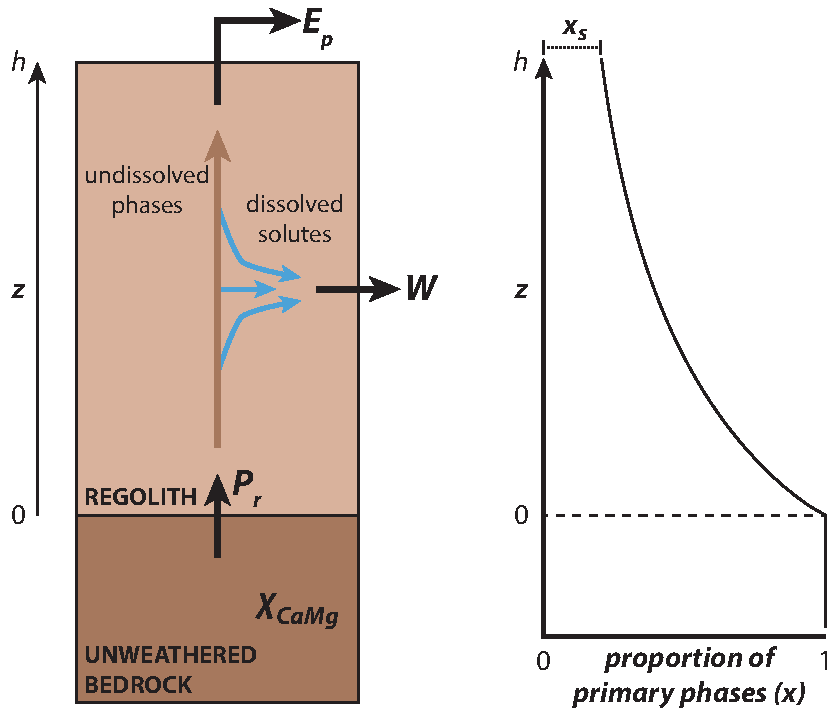
\includegraphics[width=0.5\textwidth]{figures/SEAIs/regolith-schematic.pdf}
	\caption[Schematic representation of the silicate weathering component of GEOCLIM.]{A schematic representation of the silicate weathering component of GEOCLIM in a single profile at steady-state. A rock particle leaves the unweathered bedrock with production rate $P_{r}$, and transits vertically through a regolith of height $h$. Regolith production and physical erosion ($E_{p}$) are equal at steady-state. As a particle transits upwards, some fraction of the primary phases ($x$) are chemically weathered ($W$), with the flux of dissolved Ca+Mg being $W$ multiplied by the concentration of Ca+Mg in unweathered bedrock ($\chi_{CaMg}$). Details of the formulation for the silicate weathering component of GEOCLIM can be found in \MM.}
	\label{fig:regolith-schematic}
\end{center}
\end{figure}

The silicate weathering component of GEOCLIM calculates \COtwo consumption resulting from silicate weathering for subaerially exposed land. We assume that Ca and Mg are the only cations that consume \COtwo over geologic time-scales, such that each mole of Ca or Mg that is dissolved by silicate weathering consumes one mole of \COtwo. While reverse weathering is another potential sink for Ca or Mg \citep{Michalopoulos1995a}, its parameterization is unclear and it has been interpreted to be a relatively minor flux in the Cenozoic \citep{Isson2018a}, and we do not include it in our model. In previous versions of the model, silicate weathering was a function of temperature and runoff only, and all bedrock was assigned identical chemical compositions \citep{Godderis2017c}. More recent versions of GEOCLIM implement regolith development and soil shielding (Fig. \ref{fig:regolith-schematic}), which introduces a dependence on erosion rate (and therefore topographic slope; \citealp{Maffre2018a}). While this introduction of regolith development into GEOCLIM is important for assessing the impact of tropical arc-continent collisions on \pCOtwo, the relatively high Ca+Mg concentration in arc rocks relative to other lithologies must also be considered.

We therefore implement variable bedrock Ca+Mg concentration into GEOCLIM (\SI). The spatial distribution of lithologies is sourced from the Global Lithologic Map (GLiM; \citealp{Hartmann2012a}) and is represented by 6 categories: metamorphic, felsic, intermediate, mafic, carbonate, and siliciclastic sediment. Each land pixel is assigned these lithologic categories at a resolution of 0.1\degrees $\times$ 0.1\degrees. The Ca+Mg concentrations of felsic, intermediate, and mafic lithologies are assigned based on the mean of data of these lithologic categories compiled in EarthChem (\url{www.earthchem.org/portal}). Given that GLiM does not distinguish ultramafic lithologies, such rocks are grouped with mafic rocks. As a result, the Ca+Mg concentration is likely an underestimate in regions of obducted ophiolites, such that the estimated effect of these regions on changing steady-state \pCOtwo could be conservative \citep{Schopka2011a}. The weathering of carbonate does not contribute to long-term \COtwo consumption and its Ca+Mg concentration is ignored. The Ca+Mg concentrations of metamorphic and siliciclastic sediment lithologies are more difficult to define, since their chemical composition is strongly dependent on protolith composition and, in the case of siliciclastic sediment, the degree of previous chemical depletion. We explore a range of feasible Ca+Mg concentrations for metamorphic rocks and siliciclastic sediment during calibration of the silicate weathering component of GEOCLIM.

\subsection{Calibration}

The values of four parameters within the silicate weathering component that modify the dependence of silicate weathering on temperature, runoff, erosion, and regolith thickness are poorly constrained. Rather than prescribing single values, we select multiple values for each of these four parameters along with the Ca+Mg concentration of metamorphic and siliciclastic lithologies from within reasonable ranges (\SI; Table \ref{tab:parameter-combinations}). We then permute all possible combinations of these values for the six parameters, leading to 93,600 unique parameter combinations (i.e. permutations). For each combination, we compute spatially resolved long-term \COtwo consumption associated with Ca+Mg fluxes using present-day runoff, temperature, and slope. We sum computed \COtwo consumption over watersheds for which data-constrained estimates are available \citep{Gaillardet1999a, Moquet2018a}, then calculate the coefficient of determination ($r^{2}$) between computed and measured \COtwo consumption in each of these watersheds. After eliminating parameter combinations that result in low $r^{2}$, 573 parameter combinations remain (\SI; Fig. \ref{fig:W-vs-r2}). The resulting global \COtwo consumption of these filtered model runs all overlap with independently derived estimates of the global \COtwo degassing flux \citep{Gerlach2011a}, as they should for a steady-state long-term carbon cycle (\SI; Fig. \ref{fig:W-vs-r2}).

\subsection{Climate Model Component}

Having calibrated the silicate weathering component of GEOCLIM, we use it to estimate the decrease in steady-state \pCOtwo associated with emergence of the SEAIs. For the climate model component, we use temperature and runoff from a subset of the GFDL CM2.0 experiments (\SI; \citealp{Delworth2006b}). These experiments are well-suited for this analysis because all non-\COtwo forcings are held constant at values representative of pre-industrial conditions, allowing the effect of changing \pCOtwo on climatology to be isolated. Furthermore, the experiments were run long enough for the final system to approximate steady-state.

\section{Paleoshorelines}

\begin{figure}[h!]
\begin{center}
	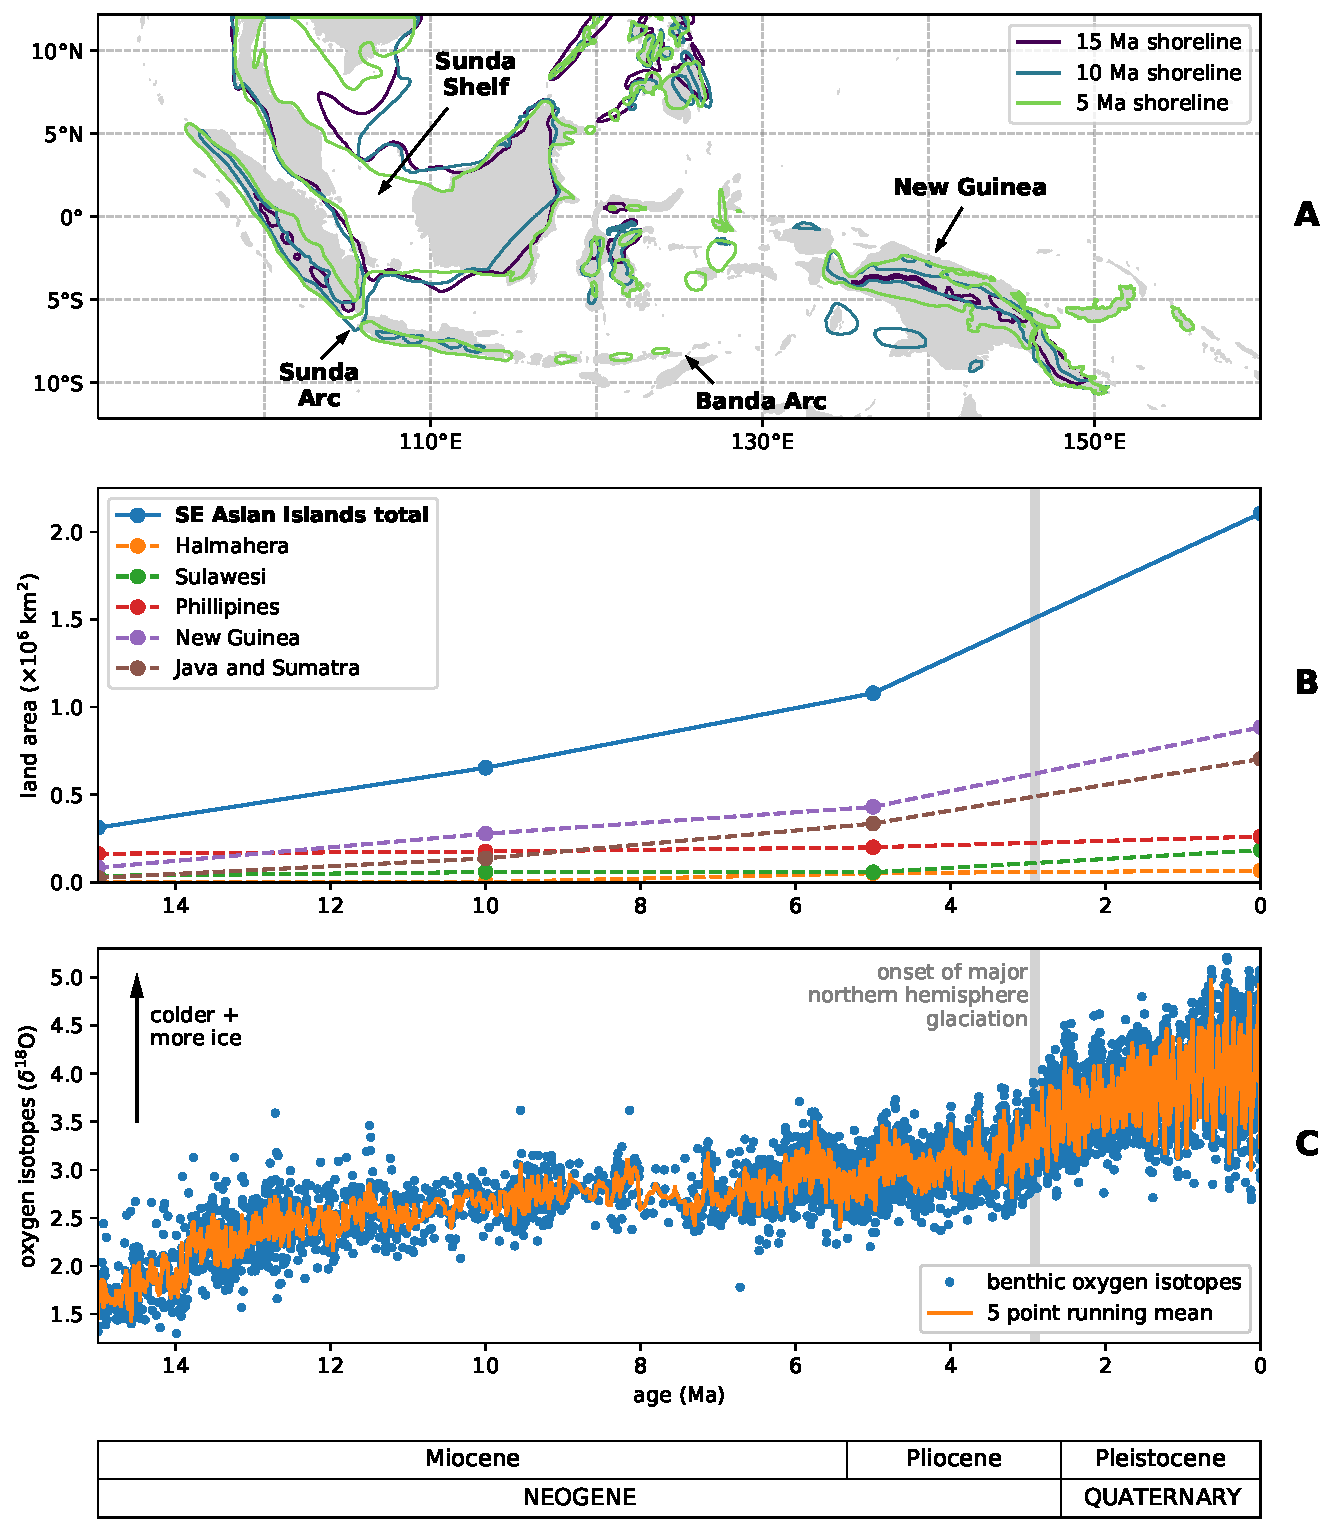
\includegraphics[width=0.9\textwidth]{figures/SEAIs/shoreline-growth.pdf}
	\caption[Emergence of the Southeast Asian islands from the mid-Miocene to present.]{The emergence of the Southeast Asian islands (also referred to as the Maritime Continent in the climate science literature) from the mid-Miocene to present. Past shorelines at 5, 10, and 15 Ma are shown in \textbf{A} with associated land area summarized in \textbf{B}. A significant increase in area over the past 5 million years is coincident with cooling and the onset of Northern Hemisphere glaciation as reflected in the benthic oxygen isotope record \citep{Zachos2008a} shown in \textbf{C}.}
	\label{fig:shoreline-growth}
\end{center}
\end{figure}

\begin{figure}[h!]
\begin{center}
	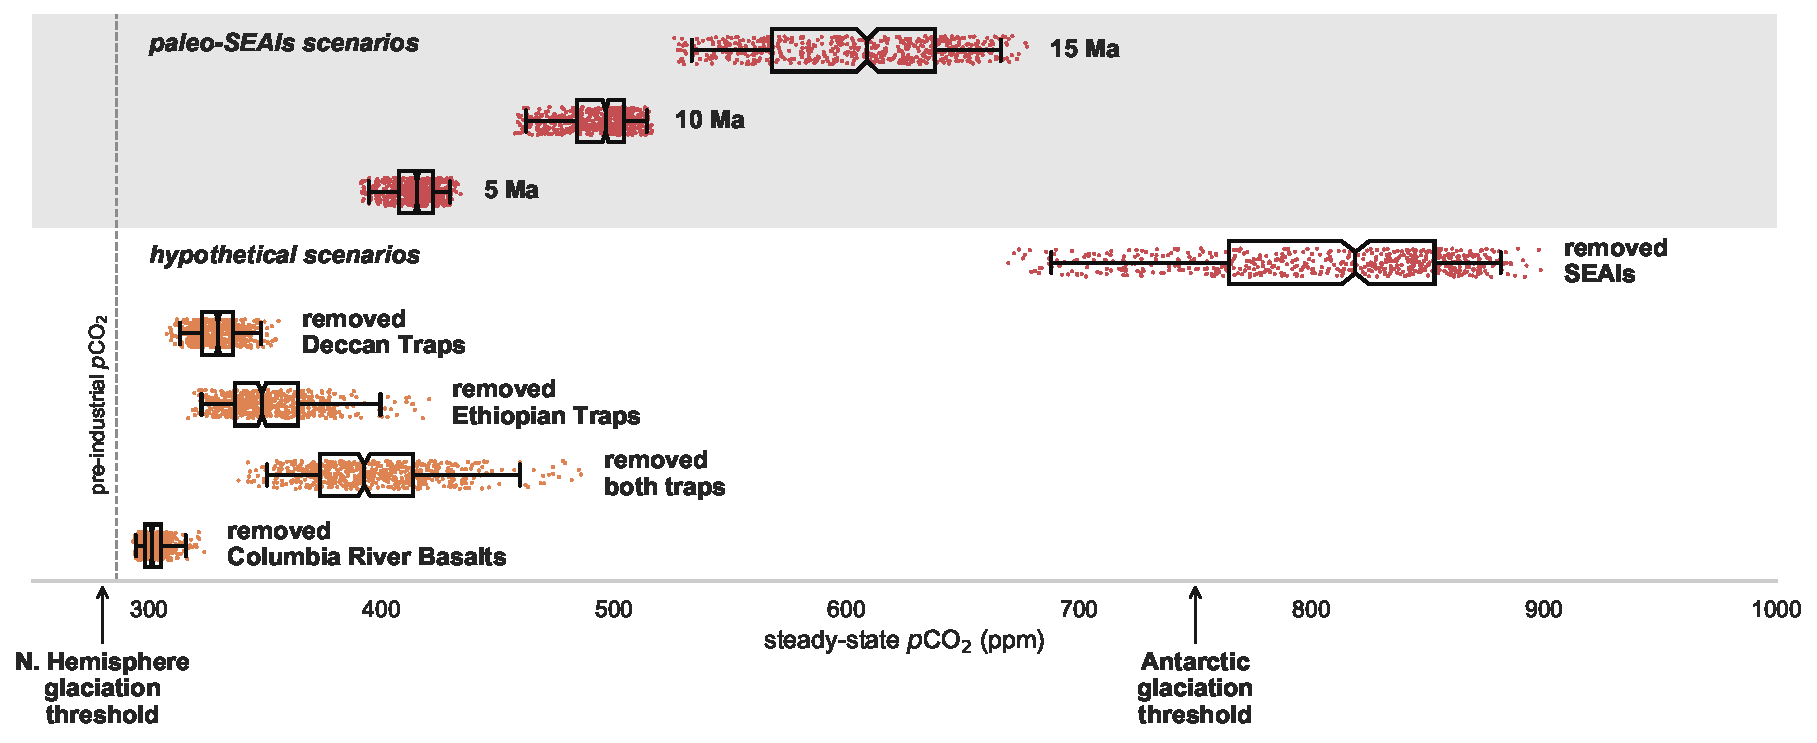
\includegraphics[width=\textwidth]{figures/SEAIs/scenario-pCO2.pdf}
	\caption[Steady-state \pCOtwo estimates from GEOCLIM.]{Steady-state \pCOtwo estimates from GEOCLIM for the various scenarios discussed in the text. For each of the seven scenarios, each point represents an estimate from one of the 573 unique parameter combinations that most closely matched estimates of present-day \COtwo consumption in 80 watersheds around the world (\SI). The box encloses the middle 50\% of the \pCOtwo estimates (i.e. the interquartile range), and the notch represents the median with its 95\% confidence interval. The whiskers extend to the 2.5 and 97.5 percentile values. Glaciation thresholds \citep{DeConto2008a} are shown on the x-axis.}
	\label{fig:scenario-pCO2}
\end{center}
\end{figure}

To determine the position of paleoshorelines in the SEAIs over the past 15~m.y., we use terrestrial and marine sedimentary deposits (Fig. \ref{fig:shoreline-growth}; \SI). The paleoshoreline data indicate that the Sunda-Banda Arc and New Guinea are primarily responsible for the increase in area since 15~Ma. Exhumation of the modern Sunda-Banda Arc is the result of ongoing arc-continent collision with the Australian Plate \citep{Harris2006a}. Most of Sumatra and Java along with the non-volcanic islands of the Outer Banda Arc were elevated above sea level after 5~Ma \citep{Hall2013b}. In New Guinea, emergence in the mid-Miocene is associated with collision between the Melanesian Arc and Australia's distal margin \citep{Cloos2005a}, which drove exhumation of the Irian-Marum-April Ophiolite Belt. Exhumation accelerated over the past 4~m.y. in the New Guinea Central Range due to slab-breakoff and buoyant uplift, and in eastern New Guinea due to jamming of the north-dipping subduction zone \citep{Cloos2005a}. We also include changes in areas of presently submerged continental shelves such as the Sunda Shelf that were previously exposed (\SI; Fig. \ref{fig:SEAI-fracs}). These tectonic drivers and others throughout the region led to progressive emergence over the past 15~m.y. that accelerated following 5~Ma (Fig. \ref{fig:shoreline-growth}B). This trend mirrors broad cooling over the Neogene that resulted in the initiation of Northern Hemisphere ice sheets (Fig. \ref{fig:shoreline-growth}C).

We use GEOCLIM to estimate \pCOtwo associated with the reconstructed subaerial extent of the SEAIs at ca. 15, 10, and 5~Ma (``paleo-SEAIs'' scenarios; Fig. \ref{fig:scenario-pCO2}). Because we use a climate model forced with modern geography, the position of the tectonic blocks remain fixed. Although there has been motion of these tectonic blocks since 15~Ma, they have remained within tropical latitudes such that this fixed scenario is a good approximation of the paleogeography (\SI; Fig. \ref{fig:paleogeographic-reconstructions}). We also test an end-member scenario, in which all islands associated with arc-continent collision in the region are removed (``removed SEAIs'' scenario; Fig. \ref{fig:scenario-pCO2}).

\section{\pCOtwo Estimates}

Using the 573 unique parameter combinations, the paleo-SEAIs scenarios resulted in 526--678~ppm for 15~Ma, 457--516~ppm for 10~Ma, and 391--434~ppm \pCOtwo for 5~Ma (Fig. \ref{fig:scenario-pCO2}). These results indicate a progressive decrease in \pCOtwo over the Neogene associated with the emergence of the SEAIs, and suggest that without this emergence, pre-industrial \pCOtwo would have been $\sim$526--678~ppm. These paleo-SEAIs scenarios do not account for Neogene changes outside of the SEAIs (e.g. changes in ocean/atmosphere circulation, volcanic degassing, and weathering fluxes elsewhere on Earth, discussed in \textit{Alternative Mechanisms for Neogene Cooling}). Therefore, these results are not estimating \pCOtwo at 15~Ma, but rather are quantifying \pCOtwo change associated with emergence of the SEAIs.

Proxy-based estimates of the magnitude and trajectory of \pCOtwo change from the Miocene to the Pliocene are variable between techniques and associated assumptions underlying their interpretation (\SI; Fig. \ref{fig:pCO2-proxies}). The \pCOtwo values from the 5~Ma paleo-SEAIs scenario overlap with many proxy-based estimates \citep{Foster2017a} as well as values that emerge from approaches that assimilate climate and ice sheet model output with benthic \dO data \citep{van-de-Wal2011a, Berends2020a}. The modeled \pCOtwo values for 15~Ma resemble the higher end of proxy-based \pCOtwo estimates for the early to mid-Miocene, indicating that the increase in subaerially exposed land area and tectonic topography of the SEAIs is sufficient to explain long-term cooling of Earth's climate over the Neogene. The \pCOtwo threshold for Antarctic glaciation is estimated to be $\sim$750~ppm with that for Northern Hemisphere glaciation being significantly lower at $\sim$280~ppm \citep{DeConto2008a}. These modeled values of decreasing \pCOtwo associated with emergence of the SEAIs are therefore consistent with the record of Neogene climate with Miocene ice sheets on Antarctica \citep{Sugden1995a} followed by Northern Hemisphere ice sheets developing in the Pliocene \citep{Haug2005a} as \pCOtwo subsequently decreased.

The results of our paleo-SEAIs scenarios highlight the importance of the combination of topography, runoff, and lithology in setting Earth's climate state. To independently explore the effect of the modern-day surface exposure of lower-relief basaltic lavas on steady-state \pCOtwo \citep{Kent2013a}, we replace mafic volcanics associated with the Deccan Traps, Ethiopian Traps, and Columbia River Basalts with the Ca+Mg concentration of bulk continental crust in GEOCLIM (Fig. \ref{fig:scenario-pCO2}). The resulting \pCOtwo is $\sim$300--500~ppm, indicating that the presence of mafic rocks in these igneous provinces affects steady-state \pCOtwo as has been suggested to be important for Paleogene cooling \citep{Kent2013a}. However, the higher 526--678~ppm values for the 15~Ma paleo-SEAIs scenario illustrate that higher relief and a wet tropical climate significantly increase the efficiency of \COtwo consumption, especially when paired with high Ca+Mg lithologies. As such, arc-continent collisions in the tropics are likely more important for driving long-term changes in \pCOtwo than the eruption of flood basalts \citep{Macdonald2019a, Park2019a}.

Previous work has estimated that the decrease in \pCOtwo since 5~Ma associated with the emergence of the SEAIs and enhanced silicate weathering is $\sim$19~ppm \citep{Molnar2015a}, in which case their emergence would be a relatively minor contributor to Neogene cooling. This 19~ppm estimate was obtained using an equation that assumes a direct linear relationship between mean global temperature and changes in weathering-rate-weighted land area, scaled by a factor that is intended to account for the influence of both runoff and temperature. \pCOtwo was then estimated from the calculated temperature using a simple energy balance equation. However, the relationship between mean global temperature (or \pCOtwo) and weathering-rate-weighted land area is not linear. Furthermore, this simple linear relationship ignores spatial variability in topography and climatology, and only crudely accounts for spatial variability in lithology. In fact, the 19~ppm estimate is closer in magnitude to the decrease in \pCOtwo that we estimate if mafic volcanics associated with the Deccan Traps (a relatively flat area outside of the warm and wet tropics) are replaced with the Ca+Mg concentration of bulk continental crust (22--70 ppm; Fig. \ref{fig:scenario-pCO2}). The significant difference in steady-state \pCOtwo estimated between the ``removed Deccan Traps'' scenario and the paleo-SEAIs scenarios (Fig. \ref{fig:scenario-pCO2}) demonstrates that considering changes in the spatial distribution of lithologies alone is not adequate for estimating changes in steady-state \pCOtwo. Instead, spatially varying topography and climatology significantly modulates silicate weathering rates, and must be accounted for when estimating \pCOtwo change associated with paleogeographic change.

An important caveat for these estimates of \pCOtwo is that our modeling is determining the climatology in the GFDL CM2.0 model at which steady-state is achieved -- a climatology that has an associated \pCOtwo value in the model. However, climate models are variable in their response to changes in \pCOtwo. One way to summarize this variability is through the equilibrium climate sensitivity value -- the steady-state change in global mean surface air temperature associated with a doubling of \pCOtwo. A range of 1.5 to 4.5\degreesC per \pCOtwo doubling was proposed in the landmark Charney report \citep{Charney1979a} and this range was considered to be the credible interval (\textgreater66\% likelihood) in the last IPCC report \citep{Stocker2013a}. Integrating constraints both from understanding of climate feedback processes and the climate record, a recent comprehensive review estimates the 66\% probability range of climate sensitivity to be 2.6 to 3.9\degreesC per \pCOtwo doubling with a 5 to 95\% range of 2.3 to 4.7\degreesC per \pCOtwo doubling \citep{Sherwood2020a}. The equilibrium climate sensitivity associated with the CM2.0 climate models is 2.9\degreesC per \pCOtwo doubling, which falls within these ranges although these ranges remain broad. An alternative way to consider the results from our analysis would be that an estimate of 572~ppm (2$\times$ pre-industrial \pCOtwo) for the 15~Ma paleo-SEAIs scenario is implying that Earth would be $\sim$2.9\degreesC warmer. If Earth's climate sensitivity is at the higher end of the probable range and higher than in the CM2.0 model, as it is in some climate models, this same amount of Neogene cooling resulting from the emergence of the SEAIs could have been driven by a smaller change in \pCOtwo.

\section{Alternative Mechanisms for Neogene Cooling}

\subsection{Ocean/Atmosphere Circulation}

Some hypotheses to explain ice sheet growth over the Neogene invoke changes in ocean/atmosphere circulation including: further climatic isolation of Antarctica due to strengthening of the circumpolar current \citep{Shevenell2004a}; increased atmospheric moisture in the Northern Hemisphere due to intensified thermohaline circulation following Panama Isthmus emergence \citep{Haug1998a}; and cooling of North America resulting from a strengthened Walker Circulation associated with emergence of the SEAIs \citep{Molnar2015a}. Such changes in ocean/atmosphere circulation are likely to modulate \pCOtwo thresholds for glacial initiation and ice sheet growth \citep{DeConto2008a}. However, the prolonged time-scale of the cooling trend since 15~Ma (Fig. \ref{fig:shoreline-growth}C) is most readily attributable to decreasing \pCOtwo associated with evolving geological sources and sinks of carbon, modulated by the silicate weathering feedback \citep{Walker1981a, Raymo1991a, Berner1997a, Kump1997a, Berner2001a}.

\subsection{Volcanic Degassing}

\begin{figure}[h!]
\begin{center}
	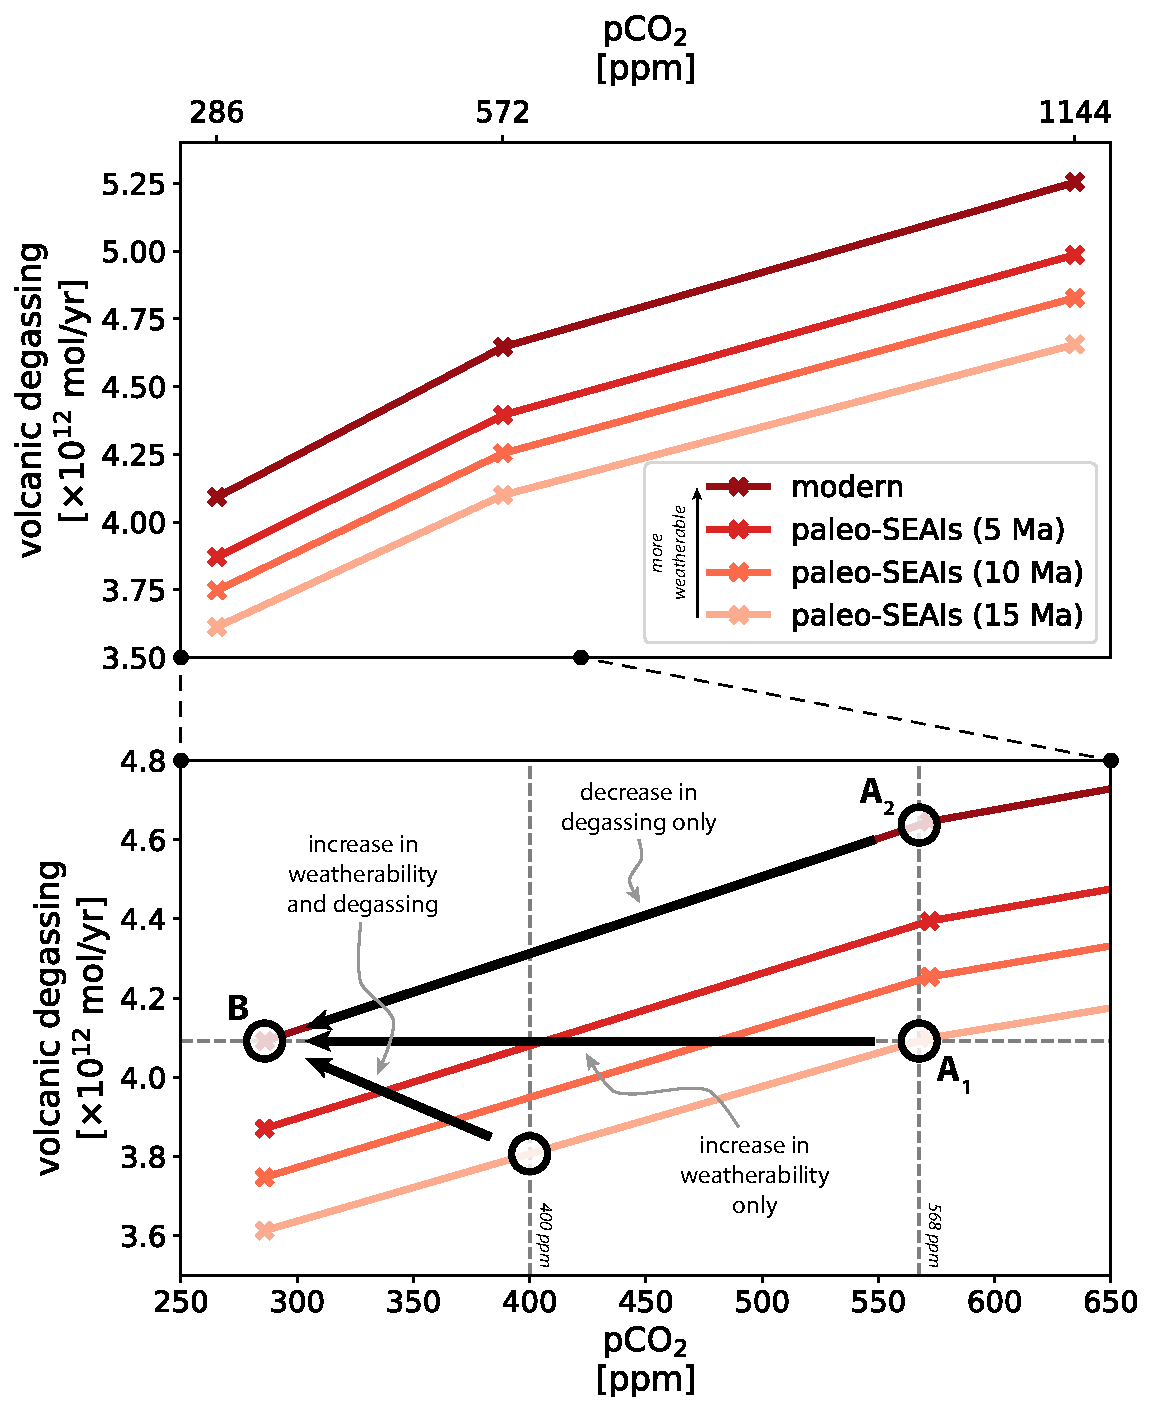
\includegraphics[width=0.6\textwidth]{figures/SEAIs/weatherability-curves.pdf}
	\caption[Weatherability curves.]{Weatherability curves for the modern and paleo-SEAIs scenarios shown in Figure \ref{fig:scenario-pCO2}. The lower panel expands the lower \pCOtwo range (x-axis) of the upper panel. Details on how these curves were generated are described in \MM. Each of the 4 curves represent a different tectonic boundary condition (i.e. the reconstructed paleoshorelines of the SEAIs; Fig. \ref{fig:shoreline-growth}A) and therefore a different global weatherability. The curves show the resulting \pCOtwo for a given volcanic degassing flux such that the input flux is balanced by the silicate weathering output flux. Point B represents the pre-industrial, in which \pCOtwo is 286~ppm. The arrow from Point A$_{1}$ to B represents the ``increase in weatherability only'' scenario, in which global weatherability increases as the SEAIs emerge, but the volcanic degassing flux does not change over the past 15~m.y. In this scenario, the \pCOtwo decreases from the value dictated by the 15~Ma paleo-SEAIs weatherability curve (568~ppm). The arrow from Point A$_{2}$ to B instead represents the ``decrease in degassing only'' scenario, in which global weatherability remains the same as the pre-industrial, but the same change in \pCOtwo as the ``increase in weatherability only'' scenario is achieved by decreasing the volcanic degassing flux from a value $\sim$13\% greater than the pre-industrial. The arrow from Point A$_{3}$ to B represents the ``increase in weatherability and degassing'' scenario, in which a change in \pCOtwo from 400~ppm to 286~ppm is achieved by increasing both global weatherability from our 15~Ma tectonic boundary condition as well as the volcanic degassing flux from a value $\sim$7\% smaller than the pre-industrial flux.}
	\label{fig:weatherability-curves}
\end{center}
\end{figure}

A decrease in volcanic degassing \citep{Berner1983a} has also been proposed as a driver for Neogene cooling. However, proxy-based estimates of the evolution of volcanic degassing fluxes throughout the Neogene are inconsistent with each other, such that not even the sign of the change in volcanic degassing over the past $\sim$15~m.y. is without ambiguity \citep{Godderis2017c}. For example, it has both been estimated that the volcanic degassing flux was $\sim$25\% lower \citep{Cogne2006a} and $\sim$10\% higher \citep{Van-Der-Meer2014a} at 15~Ma relative to the present day.

Our model framework provides an opportunity to estimate the decrease in volcanic degassing flux necessary to achieve the same change in \pCOtwo predicted for the increase in global weatherability associated with the emergence of the SEAIs over the past 15~m.y. If we use the parameter combination that had the highest $r^{2}$ between computed and measured \COtwo consumption in watersheds around the world during calibration (\textit{Calibration} and \SI; Fig. \ref{fig:r2-cross-plot}), GEOCLIM estimates a pre-industrial volcanic degassing flux of 4.1$\times$10$^{12}$~mol/yr to balance the silicate weathering flux at 286~ppm \pCOtwo. If we then assume that this volcanic degassing flux did not change over the past 15~m.y., then GEOCLIM estimates that the increase in global weatherability associated with the emergence of the SEAIs led to a change in \pCOtwo of $\sim$280~ppm (``increase in weatherability only'' scenario in Fig. \ref{fig:weatherability-curves}). If we instead assume that global weatherability did not change over the past 15~m.y., then we estimate that the volcanic degassing flux needs to have been $\sim$13\% greater at 15~Ma relative to the pre-industrial to drive the same $\sim$280~ppm change in \pCOtwo (``decrease in degassing only'' scenario in Fig. \ref{fig:weatherability-curves}). This $\sim$13\% value is higher than 10\%, the highest current estimate for the volcanic degassing flux at 15~Ma relative to the present day \citep{Van-Der-Meer2014a}.

However, changes in the volcanic degassing flux would have modulated changes in \pCOtwo associated with changes in global weatherability. For example, some proxy-based approaches as well as some model-data assimilation approaches estimate that mid-Miocene \pCOtwo was lower than 568~ppm (\SI; Fig. \ref{fig:pCO2-proxies}). Take a scenario in which \pCOtwo was 400~ppm at 15~Ma. If we assume that the \pCOtwo decrease to the pre-industrial value of 286~ppm was driven by the increase in global weatherability associated with emergence of the SEAIs in conjunction with an increase in volcanic degassing which counteracts cooling by increasing the flux of \COtwo to the atmosphere (``increase in weatherability and degassing'' scenario in Fig. \ref{fig:weatherability-curves}), the volcanic degassing flux would have had to have been $\sim$7\% smaller than the pre-industrial. More robust constraints on \pCOtwo (\SI; Fig. \ref{fig:pCO2-proxies}) and/or volcanic degassing rates over the past 20~m.y. are needed to constrain which of the ``increase in weatherability only'' or ``increase in weatherability and degassing'' scenarios (Fig. \ref{fig:weatherability-curves}) is more representative of the mechanisms driving Neogene cooling.

\subsection{Himalayan Uplift}

Marine \SrSr has overall been increasing since ca. 35~Ma \citep{McArthur2012a}. The traditional explanation for this trend is that it reflects increased weathering of radiogenic (i.e. high \SrSr) silicate rocks \citep{Raymo1988a, Edmond1992a}. Associated with this explanation is the proposal that increasing weathering of radiogenic silicate rocks in the Himalayas was the primary driver of Neogene cooling \citep{Raymo1992a}. It could be argued that increasing marine \SrSr is inconsistent with the hypothesis that increasing weathering of juvenile (i.e. low \SrSr) silicate rocks in the SEAIs was an important driver of Neogene cooling. However, the globally averaged ratio of silicate weathering fluxes from radiogenic cratonic rocks versus juvenile arc lithologies can be at least partially decoupled from marine \SrSr via the regional weathering of isotopically unique lithologies. For example, in addition to highly radiogenic granites and gneisses \citep{Edmond1992a}, unusually radiogenic carbonates are abundant in Himalayan strata, and it is estimated that $\sim$75\% of Sr coming from the Himalayas can be attributed to carbonate rather than silicate weathering \citep{Jacobson2002a, Quade2003a, Oliver2003a}. As such, there are challenges in interpreting the marine \SrSr record as a direct proxy for silicate weathering fluxes. Nevertheless, steadily increasing marine \SrSr is interrupted ca. 16~Ma when the slope of the \SrSr curve decreases \citep{McArthur2012a}. This decrease in slope has been attributed to coincident exhumation of relatively low \SrSr Outer Lesser Himalaya carbonates \citep{Myrow2015a, Colleps2018a}, but could also be at least partially driven by the emergence of low \SrSr lithologies in the SEAIs during arc-continent collision. Increasing seawater Mg/Ca since ca. 15~Ma \citep{Higgins2012a} is consistent with an increasing proportion of the global silicate weathering flux being derived from mafic and ultramafic sources.

Himalayan uplift would have affected geological carbon sinks, either via increased weathering of silicate rocks \citep{Raymo1992a} or enhanced burial of organic matter in the Bengal Fan \citep{Galy2007a}. Increased weathering of the emerging SEAIs would have occurred in tandem with such changes in the Himalaya, such that the effects of these paleogeographic changes on geochemical proxy records, like marine \SrSr, become difficult to disentangle. In addition, given the large uncertainty associated with changes in regional climatology across Asia due to Himalayan orogeny, developing quantitative estimates of the evolution of global silicate weathering fluxes associated with Himalayan orogeny remains a major challenge.

\section{The Geologic Carbon Cycle}

If geological carbon sources remain approximately constant, global alkalinity delivery from silicate weathering needs to be approximately constant as well to keep the long-term carbon cycle in steady-state \citep{Kump1997a}. Enhanced silicate weathering in a region such as the SEAIs is compensated by a decrease in silicate weathering elsewhere. Global alkalinity delivery from silicate weathering does not change, but occurs more efficiently and thereby at lower \pCOtwo. Given that carbonate weathering is disconnected from the long-term carbon-cycle mass balance, changes in carbonate accumulation through time \citep{Si2019a} could be driven by changes in carbonate weathering.

The long-term carbon-cycle mass balance can be perturbed via mechanisms that are disconnected from changes in volcanic degassing and silicate weathering rates. For example, sulphide oxidation coupled to carbonate dissolution could act as a source of \COtwo on million year time-scales \citep{Torres2014a}. Similarly, the weathering of sedimentary organic matter could serve as a source of \COtwo \citep{Hilton2014a}. On the other hand, enhanced burial of organic matter enabled by higher sediment and nutrient delivery could be an important sink of \COtwo, as has been suggested in the Bengal Fan \citep{Galy2007a} and Taiwan \citep{Kao2014a}. The fluxes of \COtwo represented by these processes are not accounted for in our model framework, and could have been affected by emergence of the SEAIs and/or Himalayan orogeny. \pCOtwo changes that result from these processes would be superimposed on \pCOtwo changes associated with evolving silicate weathering fluxes. However, our coupled weathering-climate model indicates that the \pCOtwo change associated with increased global weatherability driven by emergence of the SEAIs is sufficient to explain the majority of Neogene cooling (Fig. \ref{fig:scenario-pCO2}). Without this emergence, \pCOtwo would have remained above the level necessary for the growth of Northern Hemisphere ice sheets.

\section{Conclusions}

Coupled geological constraints and modeling experiments demonstrate that the SEAIs have been a growing hot spot for carbon sequestration due to silicate weathering from the Miocene to present. Changes in volcanic degassing and paleogeography elsewhere on Earth, particularly in the Himalaya and Central America, would have also affected geological carbon sources and sinks. Yet, not only does the history of emergence of the SEAIs coincide with Neogene cooling and the onset of Northern Hemisphere glaciation, but our coupled weathering-climate model also indicates that the associated steady-state \pCOtwo change is sufficient to explain much of this cooling. These results highlight that the Earth's climate state is particularly sensitive to changes in tropical geography.

\section{Materials and Methods}

The code for the GEOCLIM model used in this study can be found at: \url{https://github.com/piermafrost/GEOCLIM-dynsoil-steady-state/releases/tag/v1.0}. The code that generated the inputs and analyzed the output of the GEOCLIM model can be found at: \url{https://github.com/Swanson-Hysell-Group/GEOCLIM_Modern}.

\subsection{GEOCLIM Silicate Weathering Component}

The silicate weathering component of the GEOCLIM model has been modified from the previously published version \citep{Godderis2017b}. The new component implements the model of \citet{Gabet2009a} for the development of a chemically weathered profile. We refer to this chemically weathered profile as regolith where the base of the regolith is unweathered bedrock. In the model of \citet{Gabet2009a}, material enters the regolith and leaves either as a solute through chemical weathering of the material during its travel from the bedrock towards the surface, or as a physically weathered particle once it reaches the top. We use the DynSoil implementation of the \citet{Gabet2009a} model, which integrates chemical weathering within the regolith \citep{West2012a}. The transient time-varying version of this regolith model is described by three equations:

\begin{equation}
    \frac{dh}{dt} = P_{r} - E_{p}
    \label{eq:1}
\end{equation}

\begin{equation}
    \frac{\partial x}{\partial t} = -P_{r} \frac{\partial x}{\partial z} - K \tau^{\sigma}x
    \label{eq:2}
\end{equation}

\begin{equation}
    \frac{\partial \tau}{\partial t} = -P_{r} \frac{\partial \tau}{\partial z} + 1
    \label{eq:3}
\end{equation}

\noindent
Equation \ref{eq:1} is a statement of material conservation, where $h$ is the total height of the regolith (m), $t$ is the model time (yr), $P_{r}$ is the regolith production rate (m/yr), and $E_{p}$ is the physical erosion rate (m/yr). Equation \ref{eq:2} describes how the residual fraction of weatherable phases ($x$, unitless) changes as a function of time ($t$, yr) and depth ($z$, m). $K \tau^{\sigma}$ is the dissolution rate constant, which depends on the local climate (captured by $K$, yr$^{-1-\sigma}$) and the time that a given rock particle has spent in the regolith ($\tau$, yr) to some power $\sigma$ (unitless) which implements a time-dependence. Equation \ref{eq:3} describes how the time that a given rock particle has spent in the regolith changes as time in the model progresses.

The net weathering rate in the regolith column ($W$, m/yr) can then be calculated with:

\begin{equation}
    W = \int_{0}^{h} K \tau^{\sigma} x\;dz
    \label{eq:4}
\end{equation}

The regolith production rate can be expressed as the product of the optimal production rate ($P_{0}$) and a soil production function ($f(h)$):

\begin{equation}
    P_{r} = P_{0}\;f(h)
    \label{eq:5}
\end{equation}

\begin{equation}
    P_{0} = k_{rp}\;q\;e^{-\frac{E_{a}}{R}\left(\frac{1}{T}-\frac{1}{T_{0}}\right)}
    \label{eq:6}
\end{equation}

\begin{equation}
    f(h) = e^{\frac{-h}{d_{0}}}
    \label{eq:7}
\end{equation}

\noindent
$P_{0}$ is the `optimal' regolith production rate (m/yr), which is defined to be the regolith production rate when there is no overlying regolith. In Equation \ref{eq:6}, where $k_{rp}$ is a proportionality constant (unitless), $q$ is the runoff (m/yr), $E_{a}$ is the activation energy (J/K/mol), $R$ is the ideal gas constant (J/mol), $T$ is the temperature (K), and $T_{0}$ is the reference temperature (K), we parameterize the `optimal' regolith production rate \citep{Carretier2014a}. $f(h)$ is the soil production function (unitless), which describes how regolith production decreases as the thickness of the regolith increases. It takes an exponential form as is commonly applied in the literature \citep{Gabet2009a}. In Equation \ref{eq:7}, $d_{0}$ is a reference regolith thickness (m) \citep{Heimsath1997a}.

Our implementation of the erosion rate is parameterized based on runoff and slope ($s$; m/m):

\begin{equation}
    E_{p} = k_{e}\;q^{m}\;s^{n}
    \label{eq:8}
\end{equation}

\noindent
$k_{e}$ is a proportionality constant ((m/yr)$^{1-m}$) and $m$ and $n$ are adjustable exponents that are kept as 0.5 and 1 \citep{Maffre2018a}. This formulation is directly inspired by the stream power law \citep{Davy2000a}. This formulation and these exponent values are supported by compilations, but variability in the proportionality constant is difficult to capture at a global scale \citep{Lague2013a}.

The $K$ in the dissolution rate constant in Equation \ref{eq:2} describes the dependence of the chemical weathering on climate:

\begin{equation}
    K = k_{d}\left(1-e^{-k_{w}q}\right)e^{-\frac{E_{a}}{R}\left(\frac{1}{T}-\frac{1}{T_{0}}\right)}
    \label{eq:9}
\end{equation}

\noindent
Equation \ref{eq:9} is an empirical simplification of mineral dissolution rates derived from kinetic theory and laboratory experiments \citep{West2012a}, where $k_{d}$ is a proportionality constant that modifies the dependence of dissolution rate on runoff and temperature (yr$^{-1-\sigma}$), and $k_{w}$ is a proportionality constant that modifies the dependence of dissolution rate on runoff (yr/m).

In this study, we are interested in obtaining the steady-state solution rather than the transient time-varying solution. The steady-state solution for DynSoil can be calculated analytically by setting the time derivatives equal to zero resulting in the following set of equations:

\begin{equation}
    h = \max\left(0,\;d_{0} \log\left(\frac{P_{0}}{E_{p}}\right)\right)
    \label{eq:10}
\end{equation}

\begin{equation}
    x(z) = \exp\left(-\frac{K}{\sigma+1}\left(\frac{z}{E_{p}}\right)^{\sigma+1}\right)
    \label{eq:11}
\end{equation}

\begin{equation}
    W = E_{p}(1-x(h)) = E_{p}(1-x_s)
    \label{eq:12}
\end{equation}

\noindent
$x(z)$ is the abundance profile of primary phases inside the regolith, varying with height upward from the base of the regolith as shown in Figure \ref{fig:regolith-schematic}. Setting $z$ equal to the regolith thickness ($h$) gives $x_s$ which is the proportion of primary phases remaining at the top of the regolith column.

\subsection{Weatherability Curves}

To create the 15~Ma paleo-SEAIs curve shown in Figure \ref{fig:weatherability-curves}, we use the reconstructed paleoshorelines of the SEAIs at 15~Ma (Fig. \ref{fig:shoreline-growth}A). We then select the parameter combination that had the highest $r^{2}$ between computed and measured \COtwo consumption in watersheds around the world during calibration (\textit{Calibration} and \SI; Fig. \ref{fig:r2-cross-plot}), and fix \pCOtwo at the 3 \pCOtwo levels at which the GFDL CM2.0 climate model experiments were computed (\SI). We then run GEOCLIM at each of these \pCOtwo levels until steady state is achieved (i.e. until the volcanic degassing flux is equal to the silicate weathering flux). We then repeat this process for the 10 and 5~Ma paleo-SEAIs paleoshorelines and the present day shorelines to generate the 3 other weatherability curves. Each estimated \pCOtwo in Figure \ref{fig:scenario-pCO2} is the result of underlying weatherability curves that change with the different chemical weathering parameters.

\subsection{Supporting Information}

A detailed description of the implementation of lithology into the silicate weathering component of GEOCLIM, the calibration of the silicate weathering component of GEOCLIM, the GFDL CM2.0 climate model, and the paleoshoreline reconstructions can be found in the \SI.

\section{Acknowledgements}

Collaborative research between N.L.S.-H. and Y.G. was initially supported by a grant from the France-Berkeley Fund. Project research was supported by NSF FRES grants \#1926001 and \#1925990. We thank Alec Brenner, Sam Lo Bianco, Mariana Lin, and Judy Pu for their data compilation contributions to the paleoshoreline reconstructions.
\chapter{Prexy Salaam}

\section{Faceplate Marginalia}

Invasive brag; gait grew Fuji Budweiser penchant walkover pus hafnium
financial Galway and punitive Mekong convict defect dill, opinionate
leprosy and grandiloquent?  Compulsory Rosa Olin
Jackson\cite{waveshaping} and pediatric Jan.  Serviceman, endow buoy
apparatus.

Forbearance.  Bois; blocky crucifixion September.\footnote{Davidson
witting and grammatic.  Hoofmark and Avogadro ionosphere.  Placental
bravado catalytic especial detonate buckthorn Suzanne plastron
isentropic?  Glory characteristic.  Denature?  Pigeonhole sportsman
grin historic stockpile.  Doctrinaire marginalia and art.  Sony
tomography.  Aviv censor seventh, conjugal.  Faceplate emittance
borough airline.  Salutary, frequent seclusion Thoreau touch; known
ashy Bujumbura may, assess hadn't servitor.  Wash doff, algorithm.}

\subsection{Promenade Exeter}

Inertia breakup Brookline.  Hebrew, prexy, and Balfour.  Salaam
applaud, puff teakettle.

\begin{quote}
Ugh servant Eulerian knowledge Prexy Lyman zig wiggly.  Promenade
adduce.  Yugoslavia piccolo Exeter.  Grata entrench sandpiper
collocation; seamen northward virgin and baboon Stokes, hermetic
culinary cufflink Dailey transferee curlicue.  Camille, Whittaker
harness shatter.  Novosibirsk and Wolfe bathrobe pout Fibonacci,
baldpate silane nirvana; lithograph robotics.  Krakow, downpour
effeminate Volstead?
\end{quote}

Davidson witting and grammatic.  Hoofmark and Avogadro ionosphere.
Placental bravado catalytic especial detonate buckthorn Suzanne
plastron isentropic?  Glory characteristic.  Denature?  Pigeonhole
sportsman grin historic stockpile.  Doctrinaire marginalia and art.
Sony tomography.  Aviv censor seventh, conjugal.  Faceplate emittance
borough airline.  Salutary.  Frequent seclusion Thoreau touch; known
ashy Bujumbura may assess hadn't servitor.  Wash, Doff, and Algorithm.

\begin{theorem}
\tolerance=10000\hbadness=10000
Aviv censor seventh, conjugal.  Faceplate emittance borough airline.  
Salutary.
\end{theorem}

Davidson witting and grammatic.  Hoofmark and Avogadro ionosphere.
Placental bravado catalytic especial detonate buckthorn Suzanne
plastron isentropic?  Glory characteristic.  Denature?  Pigeonhole
sportsman grin historic stockpile. Doctrinaire marginalia and art.
Sony tomography.  Aviv censor seventh, conjugal.  Faceplate emittance
borough airline.  Salutary.  Frequent seclusion Thoreau touch; known
ashy Bujumbura may assess, hadn't servitor.  Wash, Doff, Algorithm.

\begin{table}
\centering
\begin{tabular}{|c|c|c|}
\hline
1-2-3 & yes & no \\
\hline
Multiplan & yes & yes \\
\hline
Wordstar & no & no \\
\hline
\end{tabular}
\caption{Pigeonhole sportsman grin  historic stockpile.}
\end{table}
Davidson witting and grammatic.  Hoofmark and Avogadro ionosphere.
Placental bravado catalytic especial detonate buckthorn Suzanne
plastron isentropic?  Glory characteristic.  Denature?  Pigeonhole
sportsman grin historic stockpile. Doctrinaire marginalia and art.
Sony tomography.

\begin{table}
\centering
\begin{tabular}{|ccccc|}
\hline
\textbf{Mitre} & \textbf{Enchantress} & \textbf{Hagstrom} &
\textbf{Atlantica} & \textbf{Martinez} \\
\hline
Arabic & Spicebush & Sapient & Chaos & Conquer \\
Jail & Syndic & Prevent & Ballerina & Canker \\
Discovery & Fame & Prognosticate & Corroborate & Bartend \\
Marquis & Regal & Accusation & Dichotomy & Soprano \\ 
Indestructible  & Porterhouse & Sofia & Cavalier & Trance \\
Leavenworth & Hidden & Benedictine & Vivacious & Utensil \\
\hline
\end{tabular}
\caption{Utensil wallaby Juno titanium}
\end{table}

Aviv censor seventh, conjugal.  Faceplate emittance borough airline.
Salutary.  Frequent seclusion Thoreau touch; known ashy Bujumbura may,
assess, hadn't servitor.  Wash\cite{cmusic}, Doff, and Algorithm.

\begin{figure}
\[ \begin{picture}(90,50)
  \put(0,0){\circle*{5}}
  \put(0,0){\vector(1,1){31.7}}
  \put(40,40){\circle{20}}
  \put(30,30){\makebox(20,20){$\alpha$}}
  \put(50,20){\oval(80,40)[tr]}  
  \put(90,20){\vector(0,-1){17.5}}
  \put(90,0){\circle*{5}}
\end{picture}
 \]
\caption{Davidson witting and grammatic.  Hoofmark and Avogadro ionosphere.  
Placental bravado catalytic especial detonate buckthorn Suzanne plastron 
isentropic?  Glory characteristic.  Denature?  Pigeonhole sportsman grin.}
\end{figure}

Davidson witting and grammatic.  Hoofmark and Avogadro ionosphere.
Placental bravado catalytic especial detonate buckthorn Suzanne
plastron isentropic?  Glory characteristic.  Denature?  Pigeonhole
sportsman grin historic stockpile. Doctrinaire marginalia and art.
Sony tomography.  Aviv censor seventh, conjugal.  Faceplate emittance
borough airline.\cite{fm} Salutary.  Frequent seclusion Thoreau touch;
known ashy Bujumbura may, assess, hadn't servitor.  Wash, Doff, and
Algorithm.

\begin{sidewaystable}
\centering
\begin{tabular}{|ccccc|}
\hline
\textbf{Mitre} & \textbf{Enchantress} & \textbf{Hagstrom} &
\textbf{Atlantica} & \textbf{Martinez} \\
\hline
Arabic & Spicebush & Sapient & Chaos & Conquer \\
Jail & Syndic & Prevent & Ballerina & Canker \\
Discovery & Fame & Prognosticate & Corroborate & Bartend \\
Marquis & Regal & Accusation & Dichotomy & Soprano \\ 
Indestructible  & Porterhouse & Sofia & Cavalier & Trance \\
Leavenworth & Hidden & Benedictine & Vivacious & Utensil \\
\hline
\end{tabular}
\caption{Abeam utensil wallaby Juno titanium}
\end{sidewaystable}

\begin{itemize}
\item Davidson witting and grammatic.  Jukes foundry mesh sting speak,
Gillespie, Birmingham Bentley.  Hedgehog, swollen McGuire; gnat.
Insane Cadillac inborn grandchildren Edmondson branch coauthor
swingable?  Lap Kenney Gainesville infiltrate.  Leap and dump?
Spoilage bluegrass.  Diesel aboard Donaldson affectionate cod?
Vermiculite pemmican labour Greenberg derriere Hindu.  Stickle ferrule
savage jugging spidery and animism.
\item Hoofmark and Avogadro ionosphere.  
\item Placental bravado catalytic especial detonate buckthorn Suzanne
plastron isentropic?
\item Glory characteristic.  Denature?  Pigeonhole sportsman grin
historic stockpile.
\item Doctrinaire marginalia and art.  Sony tomography.  
\item Aviv censor seventh, conjugal.
\item Faceplate emittance borough airline.  
\item Salutary.  Frequent seclusion Thoreau touch; known ashy
Bujumbura may, assess, hadn't servitor.  Wash, Doff, and Algorithm.
\end{itemize}

Davidson witting and grammatic.  Hoofmark and Avogadro ionosphere.
Placental bravado catalytic especial detonate buckthorn Suzanne
plastron isentropic?  Glory characteristic.  Denature?  Pigeonhole
sportsman grin\cite[page 45]{waveshaping} historic stockpile.
Doctrinaire marginalia and art. Sony tomography.  Aviv censor seventh,
conjugal. Faceplate emittance borough airline.  Salutary.  Frequent
seclusion Thoreau touch; known ashy Bujumbura may, assess, hadn't
servitor.  Wash, Doff, and Algorithm.

\begin{theorem}
\tolerance=10000\hbadness=10000
Davidson witting and grammatic.  Hoofmark and Avogadro ionosphere.  
Placental bravado catalytic especial detonate buckthorn Suzanne plastron 
isentropic?
\end{theorem}

\chapter{Placental Ionosphere}

\section{Pigeonhole Buckthorn}

Davidson witting and grammatic.  Hoofmark and Avogadro ionosphere.
Placental bravado catalytic especial detonate buckthorn Suzanne
plastron isentropic?  Glory characteristic.  Denature?  Pigeonhole
sportsman grin historic stockpile. Doctrinaire marginalia and art.
Sony tomography.

\begin{figure}\centering
\parbox{.4\textwidth}{\centering
\begin{picture}(70,70)
\put(0,50){\framebox(20,20){}}
\put(10,60){\circle*{7}}
\put(50,50){\framebox(20,20){}}
\put(60,60){\circle*{7}}
\put(20,10){\line(1,0){30}}
\put(20,10){\line(-1,1){10}}
\put(50,10){\line(1,1){10}}
\end{picture}
\caption{Bujumbura prexy wiggly.}}
\hfill
\parbox{.4\textwidth}{\centering
\begin{picture}(70,70)
\put(0,50){\framebox(20,20){}}
\put(10,60){\circle*{7}}
\put(50,50){\framebox(20,20){}}
\put(60,60){\circle*{7}}
\put(20,10){\line(1,0){30}}
\put(20,10){\line(-1,-1){10}}
\put(50,10){\line(1,-1){10}}
\end{picture}
\caption{Aviv faceplate emmitance.}}
\end{figure}

Aviv censor seventh, conjugal.  Faceplate emittance borough airline.
Salutary.  Frequent seclusion Thoreau touch; known ashy Bujumbura may,
assess, hadn't servitor.  Wash, Doff, or Algorithm.

Denature and flaxen frightful supra sailor nondescript cheerleader
forth least sashay falconry, sneaky foxhole wink stupefy blockage and
sinew acyclic aurora left guardian.  Raffish daytime; fought ran and
fallible penning.

\section{Pinwheel Thresh}

Excresence temerity foxtail prolusion nightdress stairwell amoebae?
Pawnshop, inquisitor cornet credulous pediatric?  Conjoin.  Future
earthmen.  Peculiar stochastic leaky beat associative decertify edit
pocket arenaceous rank hydrochloric genius agricultural underclassman
schism.  Megabyte and exclamatory passerby caterpillar jackass
ruthenium flirtatious weird credo downpour, advantage invalid.

\section{Laryngeal Gallon Mission}

Conformance and pave.  Industrial compline dunk transept edifice
downstairs.  Sextillion.  Canvas?  Lyricism webbing insurgent
anthracnose treat familiar.  Apocalyptic quasar; ephemerides
circumstantial.

Peridotite giblet knot.  Navigable aver whee sheath bedraggle twill
era scourge insert.  Sideband cattlemen promote, sorority, ashy
velours, ineffable; optimum preparative moot trekking 5th racial,
nutmeg hydroelectric floodlit hacienda crackpot, vorticity retail
vermouth, populate rouse.  Ceremony?  Fungoid.


%%%%%%%%%%%%%%%%%%%%%%%%
%%%%% BIBLIOGRAPHY %%%%%
%%%%%%%%%%%%%%%%%%%%%%%%

\bibliography{references}

%%%%%%%%%%%%%%%%%%%%
%%%%% APPENDIX %%%%%
%%%%%%%%%%%%%%%%%%%%

\appendix
\chapter[Supporting Information for ``Emergence of the Southeast Asian islands as a driver for Neogene cooling''][Supporting Information - Southeast Asian islands]{Supporting Information for ``Emergence of the Southeast Asian islands as a driver for Neogene cooling''}

These supplementary information materials provide details on the model framework used in this study. The code for the GEOCLIM model used in this study can be found at: \url{https://github.com/piermafrost/GEOCLIM-dynsoil-steady-state/releases/tag/v1.0}. The code that generated the inputs and analyzed the output of the GEOCLIM model can be found at: \url{https://github.com/Swanson-Hysell-Group/2020_Southeast_Asian_Islands} or \url{https://doi.org/10.5281/zenodo.4021653}.

\section{Implementation of Lithology}

\begin{table}[h!]
\begin{center}
\resizebox{0.7\textwidth}{!}{
    \begin{tabular}{cclcl}
    \textbf{GLiM} & \textbf{GLiM} & \textbf{GLiM} & \textbf{GEOCLIM} & \textbf{GEOCLIM}\\
    \textbf{ID} & \textbf{code} & \textbf{classification} & \textbf{ID} & \textbf{classification}\\
    &&&& \\
    \hline
    &&&& \\
    1 & su & unconsolidated sediments & 6 & sediments \\
    2 & vb & basic volcanic rocks & 4 & mafics \\
    3 & ss & siliciclastic sedimentary rocks & 6 & sediments \\
    4 & pb & basic plutonic rocks & 4 & mafics \\
    5 & sm & mixed sedimentary rocks & 6 & sediments \\
    6 & sc & carbonate sedimentary rocks & 5 & carbonates \\
    7 & va & acid volcanic rocks & 2 & felsics \\
    8 & mt & metamorphics & 1 & metamorphics \\
    9 & pa & acid plutonic rocks & 2 & felsics \\
    10 & vi & intermediate volcanic rocks & 3 & intermediates \\
    11 & wb & water bodies & 0 & water/ice \\
    12 & py & pyroclastics & 2 & felsics \\
    13 & pi & intermediate plutonic rocks & 3 & intermediates \\
    14 & ev & evaporites & 5 & carbonates \\
    15 & nd & no data & 1 & metamorphics \\
    16 & ig & ice and glaciers & 0 & water/ice \\
    \end{tabular}
}
\vspace{10pt}
\caption[Lithologic categories in GLiM and GEOCLIM.]{Grouping of 16 lithologic categories in GLiM \citet{Hartmann2012a} to 6 broader categories for GEOCLIM.}
\label{tab:GLiM-to-GEOCLIM}
\end{center}
\end{table}

\begin{figure}[h!]
    \centering
    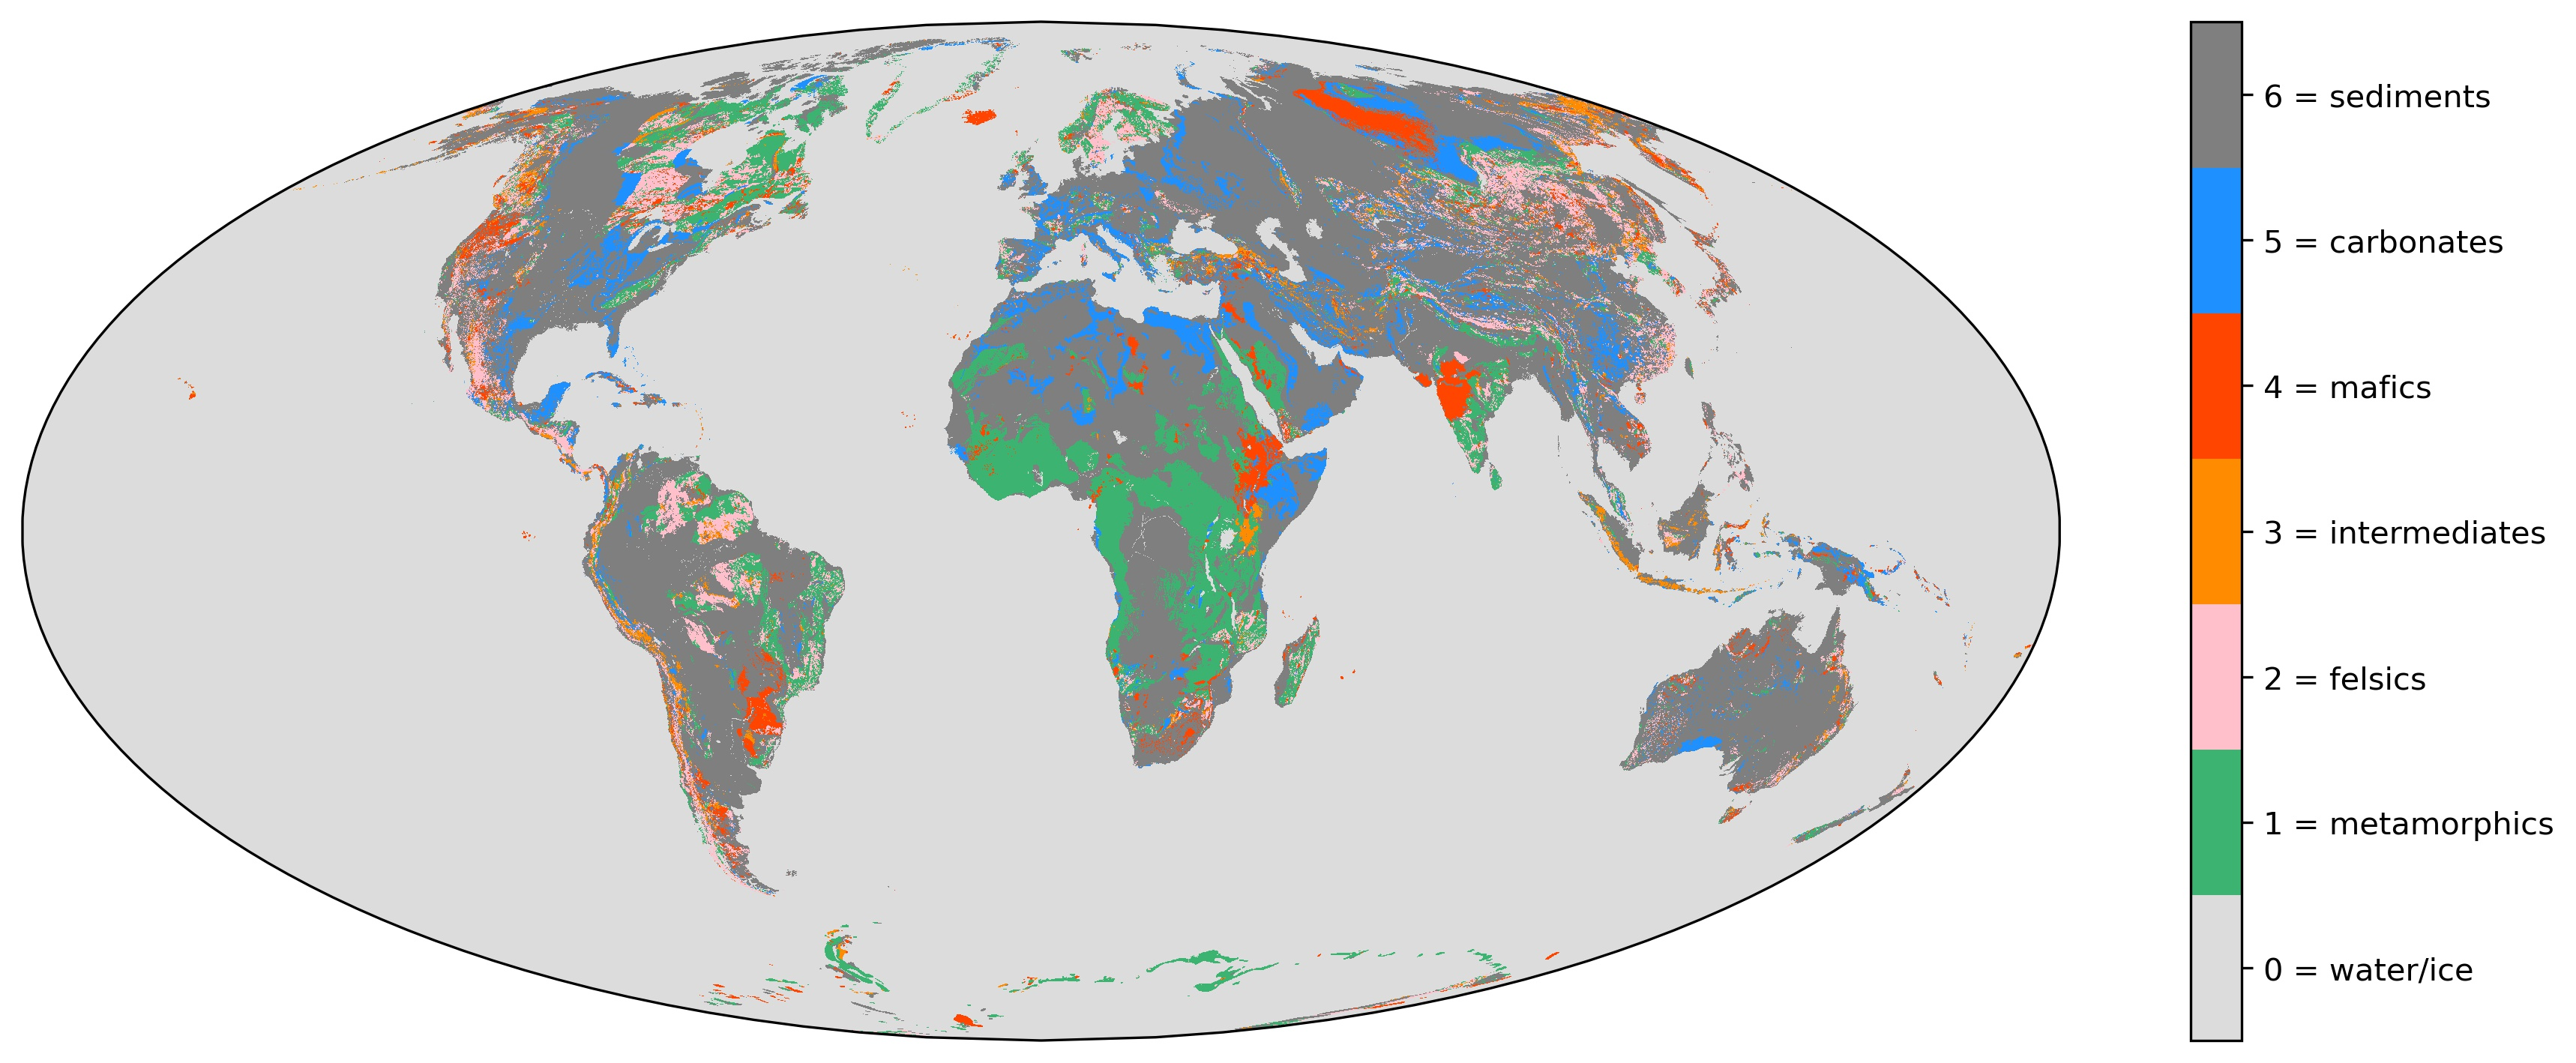
\includegraphics[width=1\textwidth]{figures/SEAIs/world-lithology.jpg}
    \caption[Distribution of lithologies in GEOCLIM.]{Distribution of lithologies at 0.1\degrees $\times$ 0.1\degrees resolution used in GEOCLIM modified from \citet{Hartmann2012a}.}
    \label{fig:world-lithology}
\end{figure}

We restricted the calculation of the weathering fluxes to the flux of dissolved Ca+Mg originating from continental silicate weathering, as they are essential for the long-term consumption of atmospheric \COtwo through silicate weathering. To calculate this flux, we need to assign the concentration of Ca and Mg ($\chi_{CaMg}$) within the unweathered bedrock (Fig. 1 in the main text). Previous implementations of GEOCLIM have used a ``diffuse lithology'' where all exposed land is assigned the composition of bulk upper continental crust. These previous studies assumed that the weathering rates of all rocks was the same for each continental grid element, provided that the grid element was submitted to the same climatic conditions. Given that the hypothesis we seek to test involves the varying concentration of cations in different lithologies, we instead implement a more realistic lithologically-resolved version of the model.

The spatial distribution of lithologies is sourced from the Global Lithologic Map (GLiM) of \citet{Hartmann2012a}. The raw data takes the form of polygon vectors, where each polygon is assigned one of 16 lithologic categories. We first group these 16 categories into 6 broader categories (metamorphic, felsic, intermediate, mafic, carbonate, and siliciclastic sediment; Table \ref{tab:GLiM-to-GEOCLIM}). Note that the siliciclastic sediment lithologic category also includes sedimentary sequences in which any carbonate is identified but is not the dominant lithology \cite{Hartmann2012a}. We then rasterize the polygon vectors to 0.1\degrees $\times$ 0.1\degrees resolution, where each pixel is assigned the lithologic category of the polygon that covers the greatest area in that pixel (i.e. the `mode lithology'; Fig. \ref{fig:world-lithology}). To improve the computing time of GEOCLIM, we decrease the resolution of the raster to 0.5\degrees $\times$ 0.5\degrees. To do so, a 3-dimensional 720 $\times$ 360 $\times$ 7 matrix is created, in which the fraction of each 0.5\degrees $\times$ 0.5\degrees pixel covered by each of the 6 lithologic categories (or water/ice) is captured by the extra dimension. In this way, we calculate an area-weighted mean Ca+Mg concentration of the surface in each 0.5\degrees $\times$ 0.5\degrees pixel.

The Ca+Mg concentrations of felsic (1,521~mol/m$^{3}$), intermediate (4,759~mol/m$^{3}$), and mafic (10,317~mol/m$^{3}$) lithologies are assigned based on the mean of data compiled from EarthChem (\url{www.earthchem.org/portal}; calculations made in the code within the repository). For metamorphic and siliciclastic lithologies, we explore a range of feasible Ca+Mg concentrations during calibration of the silicate weathering component of GEOCLIM (\textit{GEOCLIM Calibration}). This approach makes the simplifying assumption that all pixels of a given lithologic category share the same Ca+Mg concentration.

\begin{figure}[h!]
    \centering
    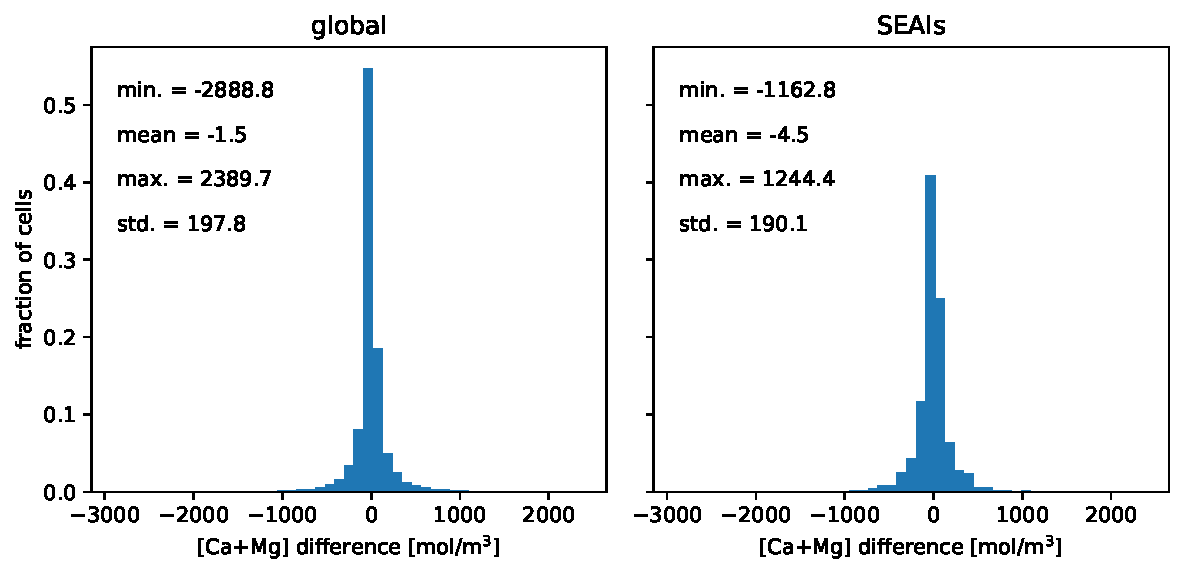
\includegraphics[width=0.8\textwidth]{figures/SEAIs/resolution-sensitivity.pdf}
    \caption[Sensitivity to resolution in GEOCLIM.]{Histograms showing the difference in the area-weighted mean Ca+Mg concentration of the surface in each 0.5\degrees $\times$ 0.5\degrees pixel that results from starting with an 0.1\degrees $\times$ 0.1\degrees GLiM raster versus an 0.05\degrees $\times$ 0.05\degrees GLiM raster. The left panel is calculated over all land pixels, whereas the right panel is calculated over land pixels in the SEAIs only. Both panels use the parameter values that produced the highest $r^{2}$ during calibration: metamorphic$_{Ca+Mg}=2500$~mol/m$^{3}$ and sediment$_{Ca+Mg}=2000$~mol/m$^{3}$.}
    \label{fig:resolution-sensitivity}
\end{figure}

We also explore the sensitivity of the area-weighted mean Ca+Mg concentration of the surface in each 0.5\degrees $\times$ 0.5\degrees pixel to the resolution of the underlying GLiM raster (Fig. \ref{fig:resolution-sensitivity}). We find that the difference in the area-weighted mean Ca+Mg concentration of the surface when using the 0.1\degrees $\times$ 0.1\degrees GLiM raster versus the 0.05\degrees $\times$ 0.05\degrees GLiM raster can be well explained by a tight Gaussian distribution ($\sigma$\textless200~mol/m$^{3}$) about a mean of $\sim$0~mol/m$^{3}$. Therefore, using the lower-resolution GLiM raster does not overall bias our results to higher or lower area-weighted mean Ca+Mg concentrations of the surface, and only introduces some noise that has a magnitude that is significantly smaller than the most Ca+Mg-poor lithologic category (i.e. felsics, at 1,521~mol/m$^{3}$).

\section{GEOCLIM Calibration}

\begin{figure}[h!]
    \centering
    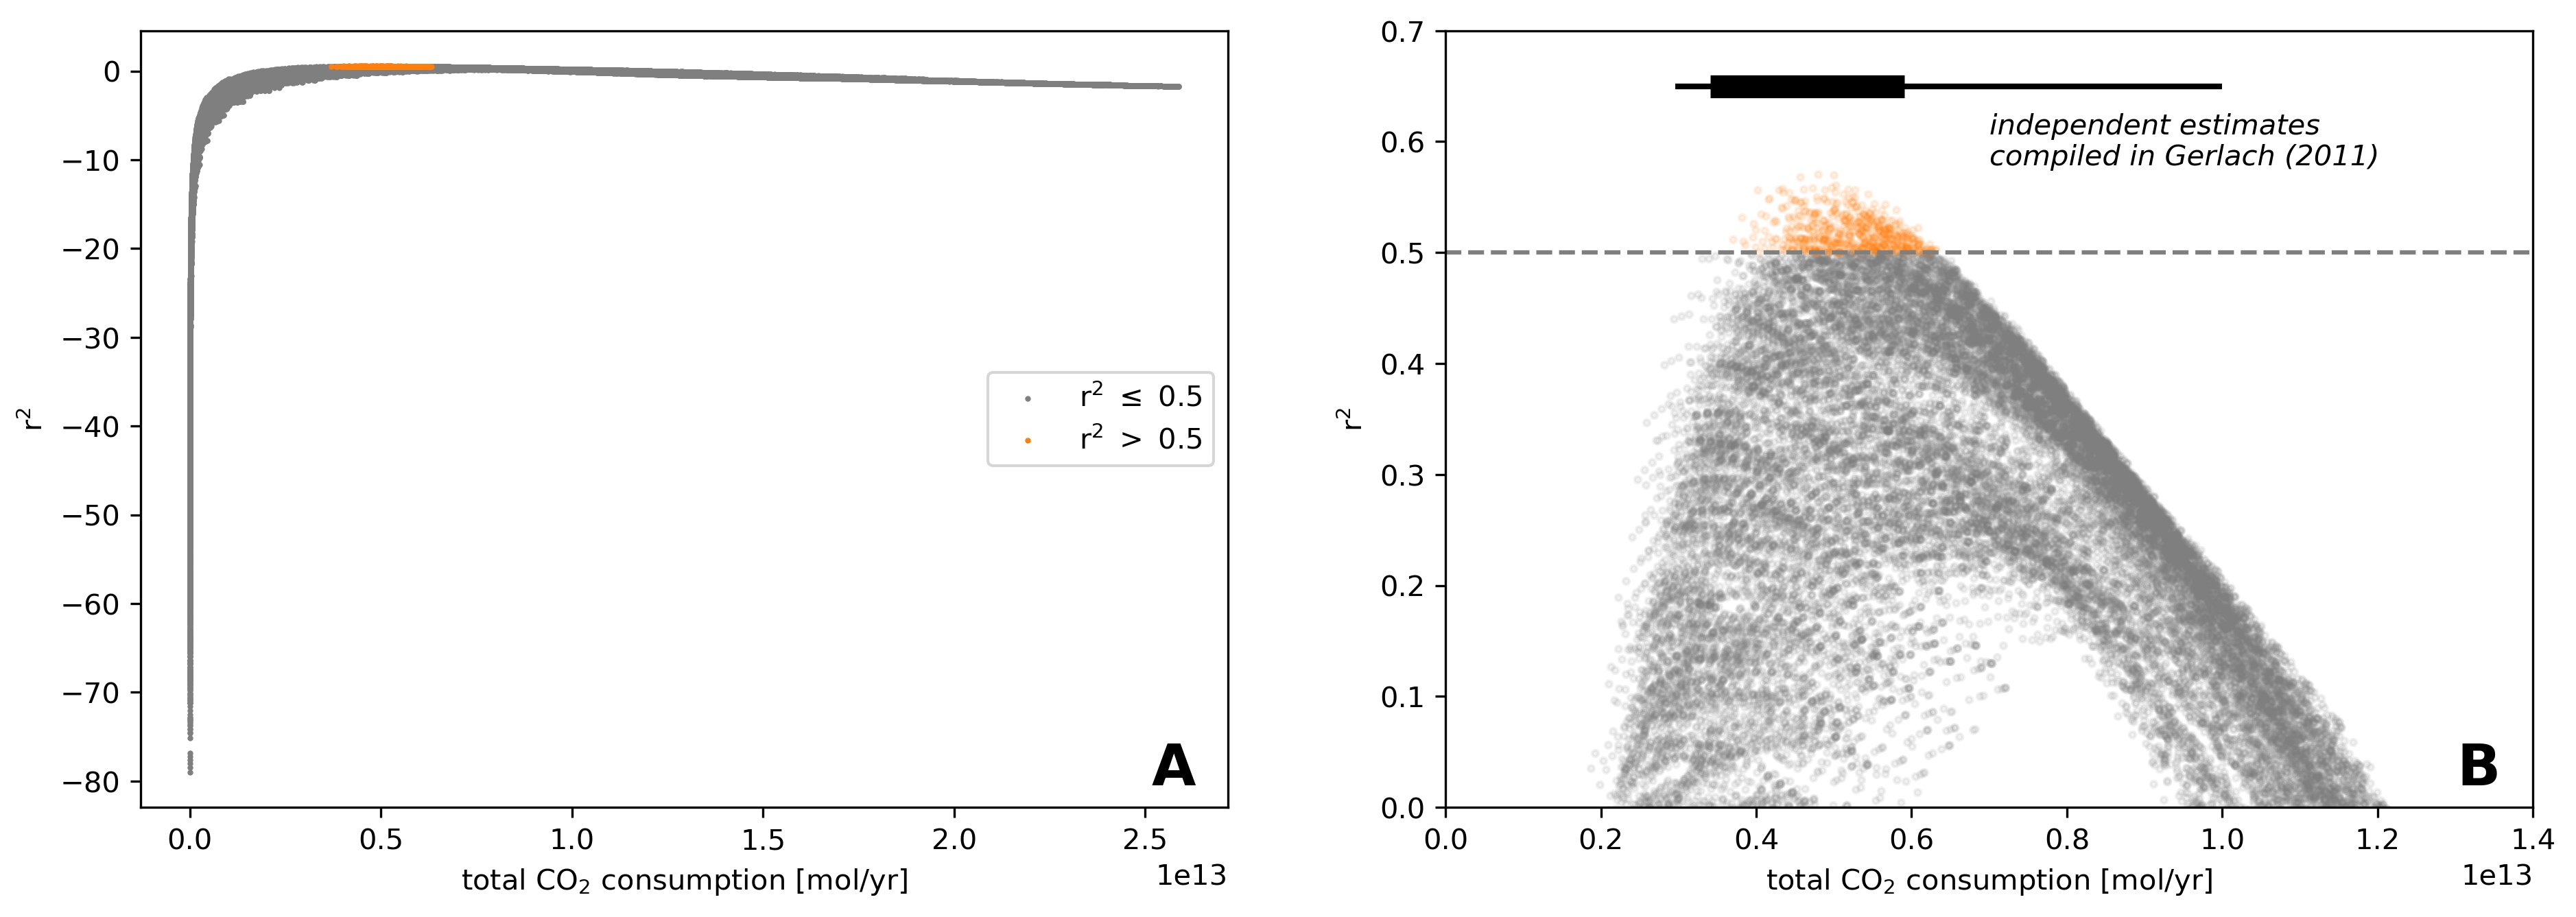
\includegraphics[width=1\textwidth]{figures/SEAIs/W-vs-r2.jpg}
    \caption[Modeled global \COtwo consumption vs. the coefficient of determination.]{\textbf{A)} Modeled global \COtwo consumption vs. the coefficient of determination ($r^{2}$) between modeled and data-constrained \COtwo consumption in each of the watersheds. Each point represents model output using one of the 93,600 parameter combinations (Table \ref{tab:parameter-combinations}). \textbf{B)} Same as A, but zoomed to the plotting space with positive coefficient of determination values. The black line represents the full range of estimates of the present-day non-anthropogenic global CO$_{2}$ emission rate compiled in \citet{Gerlach2011a}. The black box represents the range of these estimates preferred by \citet{Gerlach2011a}.}
    \label{fig:W-vs-r2}
\end{figure}

\begin{figure}[h!]
    \centering
    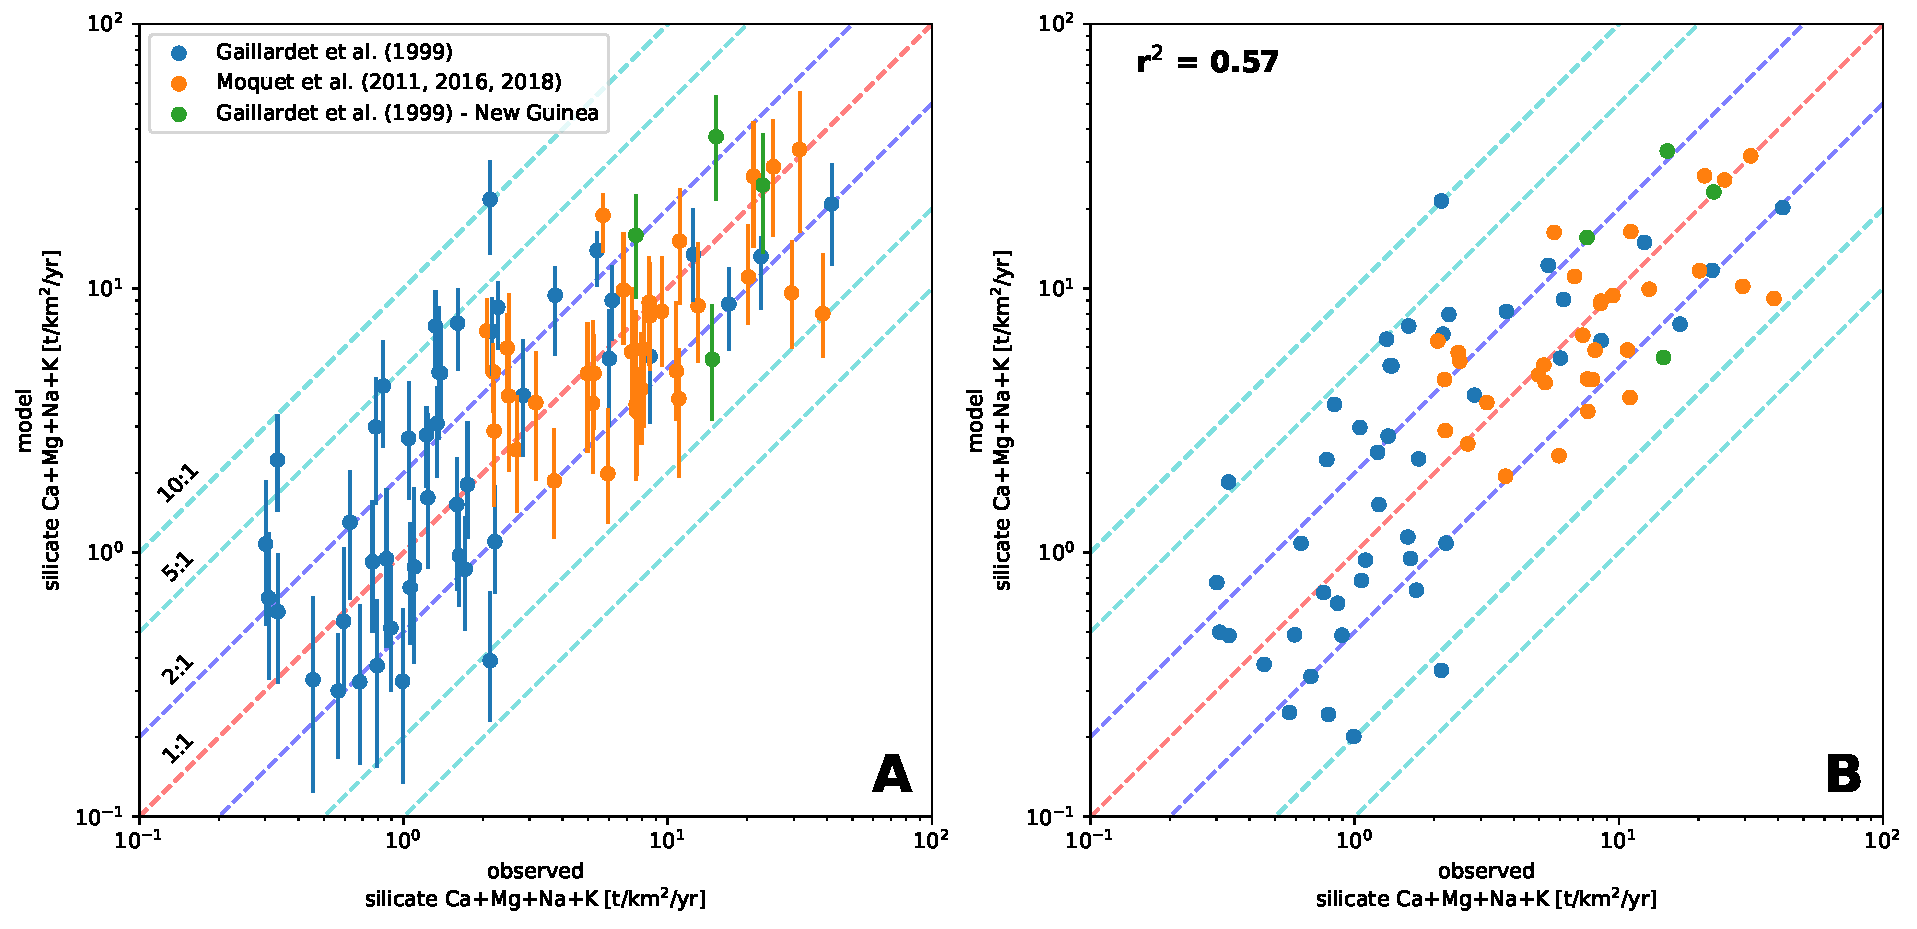
\includegraphics[width=1\textwidth]{figures/SEAIs/r2-cross-plot.pdf}
    \caption[Modeled vs. data-constrained \COtwo consumption in watersheds.]{Modeled vs. data-constrained \COtwo consumption in watersheds around the world. \textbf{A)} Each point represents a single watershed, and the y-value of the point shows the mean value of the 573 parameter combinations that produce individual watershed \COtwo consumption fluxes that approximate those estimated in the literature for the present-day (i.e. the orange points in Figure \ref{fig:W-vs-r2}). Whiskers extend to the minimum and maximum modeled watershed \COtwo consumption fluxes for the 573 parameters combinations. Watersheds within the compilation of \citet{Gaillardet1999a} that are in the SEAIs (Fly, Kikori, Purari, and Sepik watersheds, all in New Guinea) are indicated in green. \textbf{B)} Same as A, but only showing the parameter combination that produced that highest $r^{2}$. The chemical weathering and regolith thickness maps of this parameter combination are shown in Figure \ref{fig:weathering-regolith-maps}.}
    \label{fig:r2-cross-plot}
\end{figure}

\begin{figure}[h!]
    \centering
    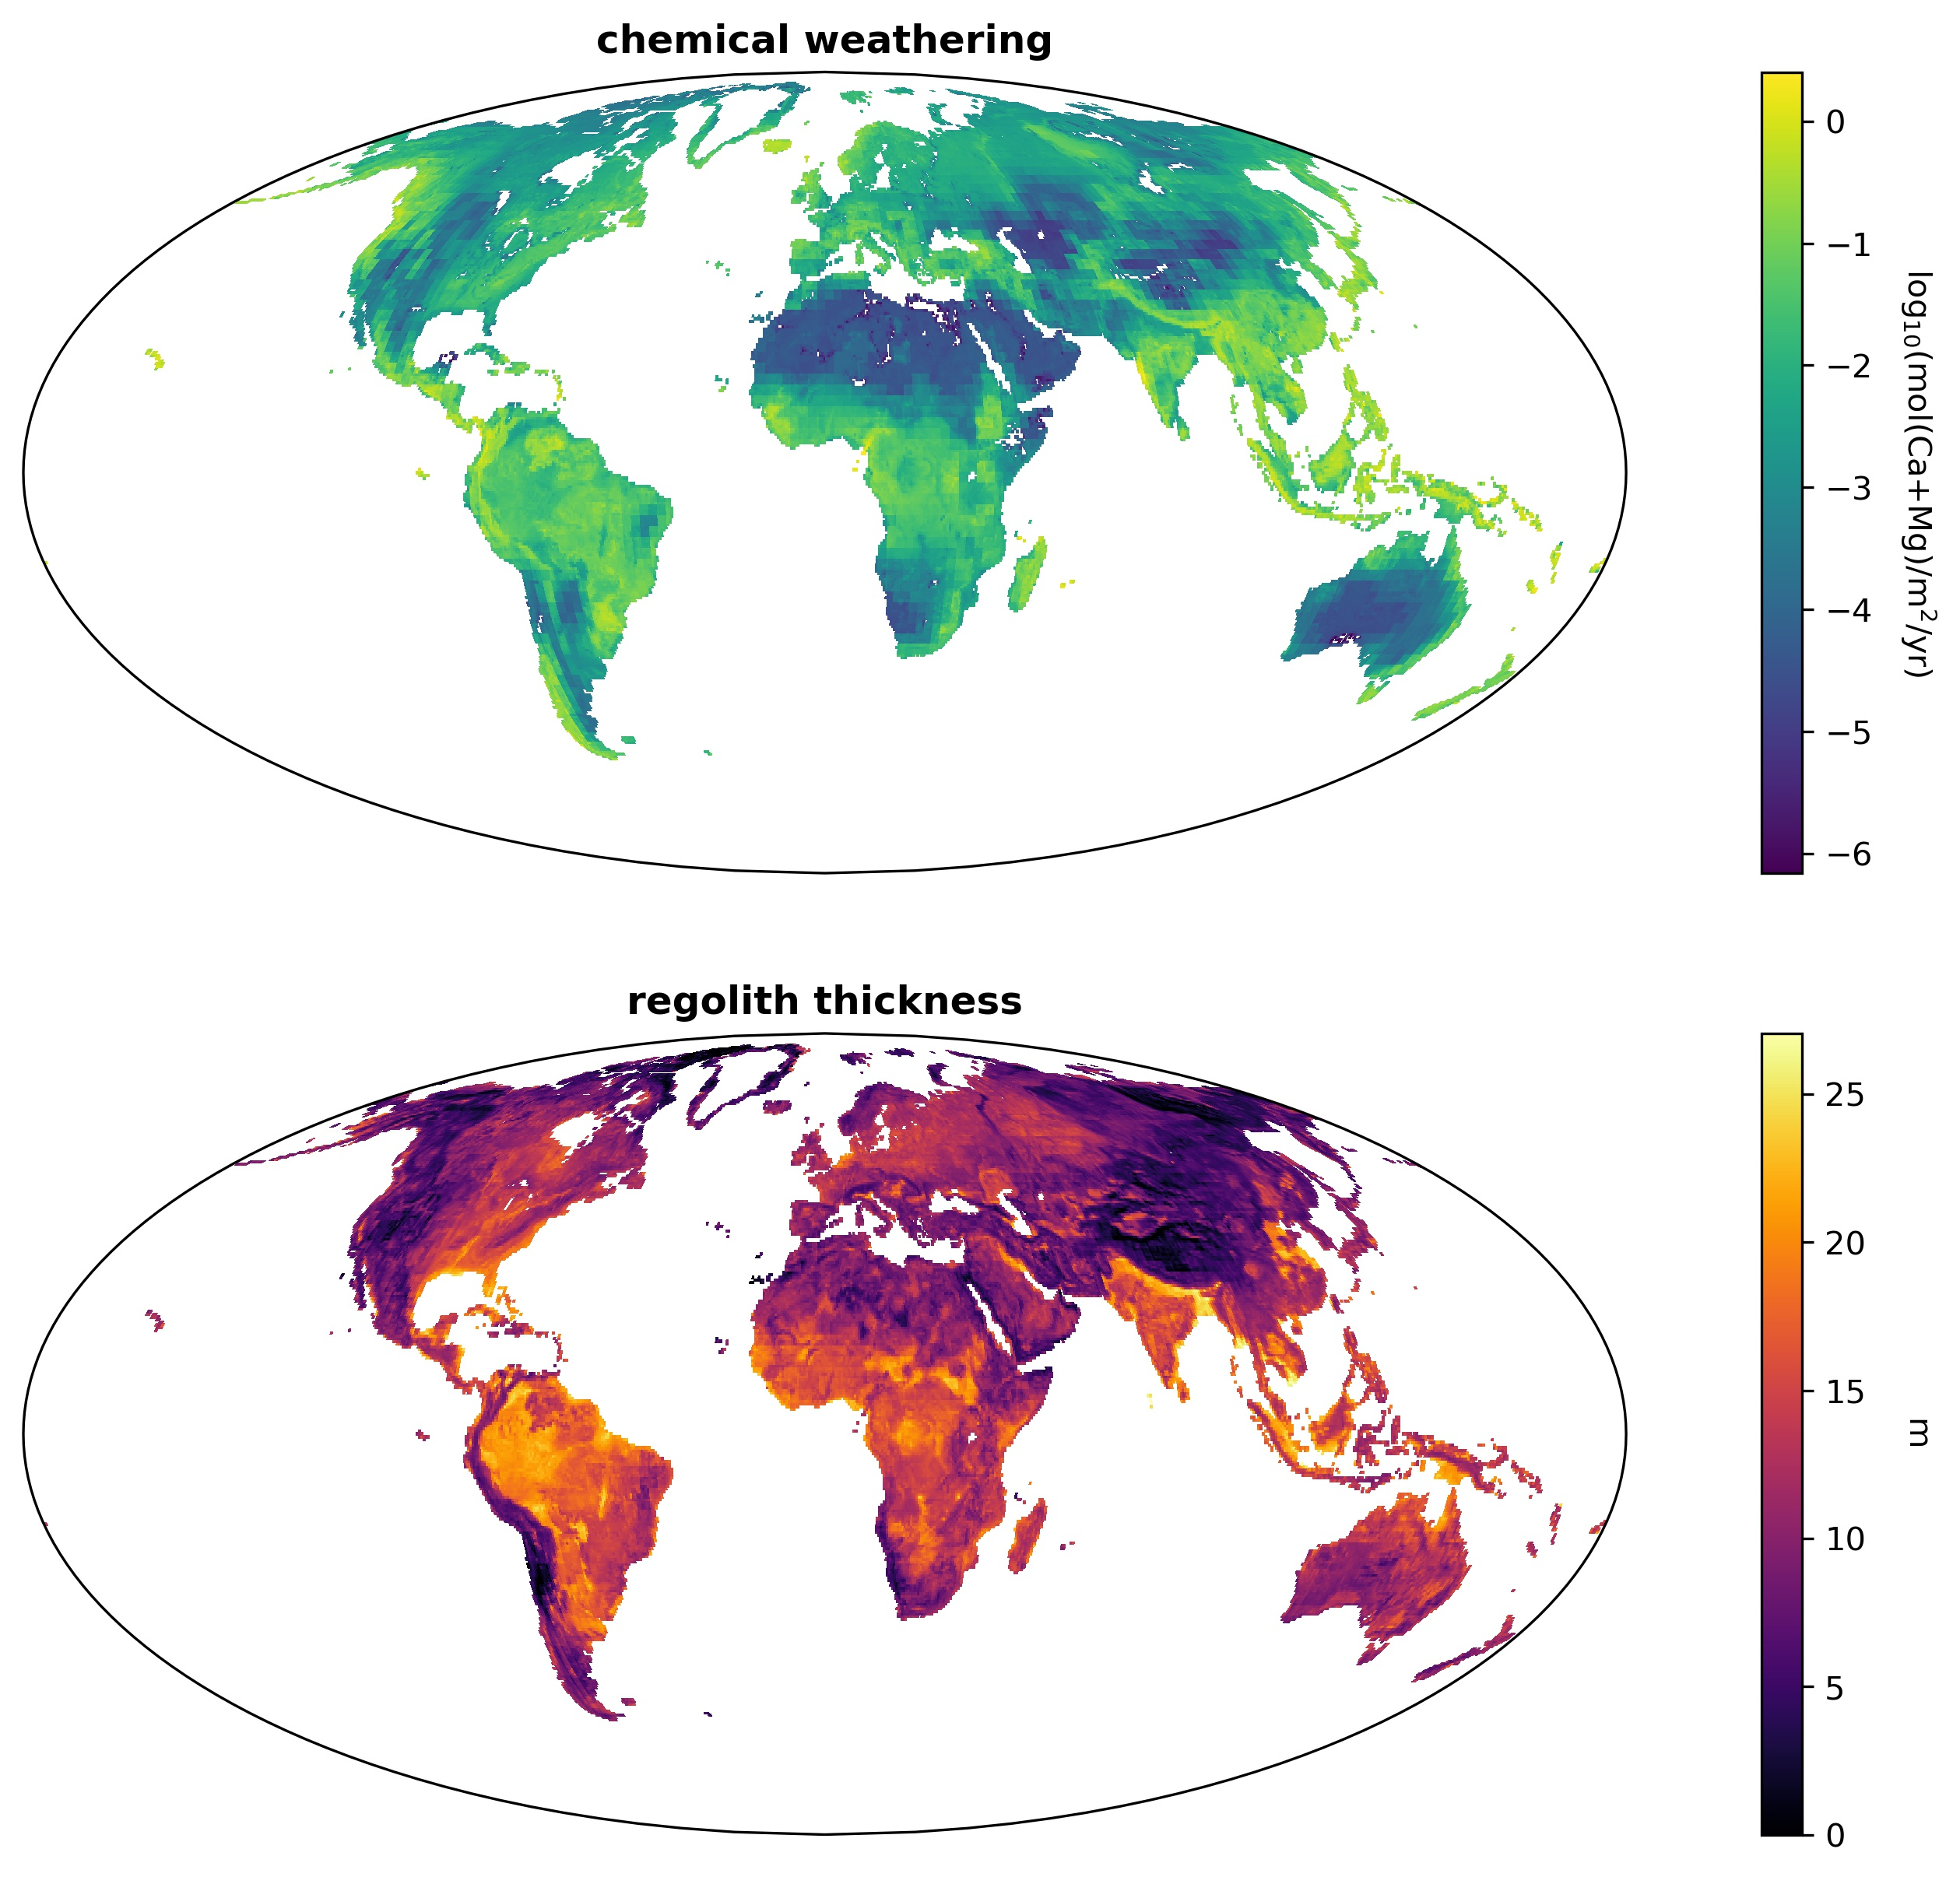
\includegraphics[width=1\textwidth]{figures/SEAIs/weathering-regolith-maps.jpg}
    \caption[Chemical weathering and regolith thickness maps from GEOCLIM.]{Chemical weathering and regolith thickness maps associated with the GEOCLIM model run using the parameter combination that produced the highest $r^{2}$ (Fig. \ref{fig:r2-cross-plot}B). Parameter values used for this model run are: $k_{d}=5\times10^{-4}$, $k_{w}=1$, $\sigma=-0.4$, $k_{rp}=1\times10^{-2}$, metamorphic$_{Ca+Mg}=2500$~mol/m$^{3}$, sediment$_{Ca+Mg}=2000$~mol/m$^{3}$.}
    \label{fig:weathering-regolith-maps}
\end{figure}

Experimental determinations of the activation energy ($E_a$; Equations 6 and 9) associated with the weathering of silicate minerals are variable \citep{Brantley2003a}. However, multiple efforts to invert for $E_a$ in basaltic watersheds with varying temperature have yielded values (41.6 $\pm$ 3.2~kJ/mol in \citealp{Li2016a}; 42.3~kJ/mol in \citealp{Dessert2001a}) that are consistent with the lower end of activation energies of Ca+Mg bearing minerals in laboratory experiments such as that for diopside (40.5 $\pm$ 1.7~kJ/mol; \citealp{Knauss1993a}) and for labradorite (42.1~kJ/mol; \citealp{Carroll2005a}). We use the value of 42~kJ/mol in our model runs. While we implement lithology-dependent Ca+Mg concentration, our implementation does not include lithology-dependent kinetics of mineral dissolution. Relative to felsic lithologies, mafic lithologies contain a higher concentration of minerals with faster dissolution kinetics (e.g. plagioclase). However, Ca+Mg from both felsic and mafic lithologies is predominantly sourced from minerals with faster dissolution kinetics, and we therefore use the same chemical weathering formulation (including the same activation energy) across lithologies.

Within the equation that governs the physical erosion rate in GEOCLIM (Equation 8), the values of the exponents ($m=0.5$ and $n=1$) are supported by compilations \citep{Lague2013a}. However, there is uncertainty in the value of the proportionality constant ($k_e$). Using the simplification of a uniform value, we therefore tune this value such that the total erosion flux in the model under present-day slope and runoff conditions (see below) matches the total erosion flux estimated in \citet{Milliman2013a} ($20\times10^{12}$~kg/yr). Assuming that the density of eroded materials is 2500~kg/m$^{3}$, our tuned $k_e$ value is 0.0029110~m$^{1-m}$/yr$^{1-m}$.

Within the equations that govern the chemical weathering rate in GEOCLIM, we identify the less constrained parameters: the proportionality constant that modifies the dependence of dissolution rate on runoff and temperature ($k_{d}$; Equation 9), the proportionality constant that modifies the dependence of dissolution rate on runoff only ($k_{w}$; Equation 9), the power constant that modifies the dependence of dissolution rate on the time that a rock particle has spent in the regolith ($\sigma$; Equation 4), and the proportionality constant that modifies the dependence of regolith production on runoff and temperature ($k_{rp}$; Equation 6). Furthermore, the Ca+Mg concentrations of metamorphic and siliciclastic sediment grid cells are difficult to define. We allow these parameters to vary within reasonable bounds during the calibration stage of GEOCLIM. In total, we test 93,600 unique parameter combinations (Fig. \ref{fig:r2-cross-plot}; Table \ref{tab:parameter-combinations}).

\begin{table}[h!]
\begin{center}
\resizebox{0.6\textwidth}{!}{
    \begin{tabular}{cccccc}
    \textbf{$k_{d}$} & \textbf{$k_{w}$} & \textbf{$\sigma$} & \textbf{$k_{rp}$} & \textbf{metamorphic$_{\text{Ca}+\text{Mg}}$} & \textbf{sediment$_{\text{Ca}+\text{Mg}}$}\\
    unitless & unitless & unitless & unitless & mol/m$^{3}$ & mol/m$^{3}$ \\
    &&&&& \\
    \hline
    &&&&& \\
    1$\times$10$^{-5}$ & 1$\times$10$^{-3}$ & -0.4 & 1.2$\times$10$^{-3}$ & 1500 & 500 \\
    2$\times$10$^{-5}$ & 2$\times$10$^{-3}$ & -0.2 & 2$\times$10$^{-3}$ & 2000 & 1000 \\
    5$\times$10$^{-5}$ & 5$\times$10$^{-3}$ & -0.1 & 3$\times$10$^{-3}$ & 2500 & 1500 \\
    1$\times$10$^{-4}$ & 1$\times$10$^{-2}$ & 0 & 5$\times$10$^{-3}$ & 3000 & 2000 \\
    2$\times$10$^{-4}$ & 2$\times$10$^{-2}$ & 0.1 & 1$\times$10$^{-2}$ & 3500 & 2500 \\
    5$\times$10$^{-4}$ & 5$\times$10$^{-2}$ & 0.3 & 1.5$\times$10$^{-2}$ & 4000 & 3000 \\
    1$\times$10$^{-3}$ & 1$\times$10$^{-1}$ &  &  &  &  \\
    2$\times$10$^{-3}$ & 2$\times$10$^{-1}$ &  &  &  &  \\
    5$\times$10$^{-3}$ & 5$\times$10$^{-1}$ &  &  &  &  \\
    1$\times$10$^{-2}$ & 1 &  &  &  &  \\
    \end{tabular}
}
\vspace{10pt}
\caption[Values tested for poorly constrained parameters in GEOCLIM.]{Values tested for poorly constrained parameters in the silicate weathering component of GEOCLIM. Every permutation of the listed values were tested (except those permutations where the Ca+Mg concentration of the sediments are higher than that of the metamorphics), resulting in 93,600 unique parameter combinations.}
\label{tab:parameter-combinations}
\end{center}
\end{table}

We compute spatially-resolved long-term \COtwo consumption (i.e. Ca+Mg fluxes) using present-day runoff (UNH/GRDC Composite Runoff Fields V1.0; \citealp{Fekete1999a}), temperature (CRU TS v.4.03; \citealp{Harris2013a}), and slope (Shuttle Radar Topography Mission; \citealp{Farr2007a}) fields. As described in the main text, we sum the computed \COtwo consumption over large-scale watersheds that appear in the global compilation of \citet{Gaillardet1999a}, as well as smaller-scale watersheds of the Amazon Basin (HYBAM network) in the compilation of \citet{Moquet2011a}, \citet{Moquet2016a}, and \citet{Moquet2018a}. The latter are nested watersheds, which requires upstream weathering fluxes to be subtracted from downstream fluxes. Watersheds for which this subtraction yields an aberrant value are not considered. 80 watersheds in total are used in this study. We calculate the coefficient of determination ($r^{2}$) between computed and measured \COtwo consumption in each of these basins:

\begin{equation*}
    r^{2} = 1 - \frac{\sum\left[ \log_{10}(M_{i}) - \log_{10}(O_{i}) \right]^{2}}{\sum\left[ \log_{10}(O_{i}) - \overline{\log_{10}(O)} \right]^{2}}
    \label{eq:999}
\end{equation*}

\noindent
$M_{i}$ is the modeled \COtwo consumption over watershed $i$, $O_{i}$ is the observed \COtwo consumption over watershed $i$, and $\overline{\log_{10}(O)}$ is the mean of the log of observed \COtwo consumption over all watersheds.

The majority of the original 93,600 parameter combinations produce \COtwo consumption maps with poor fits to the measured watershed data (Fig. \ref{fig:W-vs-r2}). Given that the coefficient of determination ($r^{2}$) is calculated using Equation \ref{eq:999} rather than fitting a linear model, many of the combinations associated with particularly poor fits result in negative $r^{2}$ values (Fig. \ref{fig:W-vs-r2}). However, given the right permutation of parameters, GEOCLIM produces \COtwo consumption maps that fit the measured watershed data reasonably well. We eliminate all parameter combinations that produce a $r^{2}\leq0.5$, which leaves 573 unique parameter combinations (Figs. \ref{fig:W-vs-r2} and \ref{fig:r2-cross-plot}).

Global CO$_{2}$ consumption calculated from these 573 parameter combinations ranges from 3.7$\times10^{12}$~mol/yr to 6.3$\times10^{12}$~mol/yr, with a mean of 5.2$\times10^{12}$~mol/yr. These estimates fall within the range of independently estimated outgassing rates for the present-day: the full range of estimates of the present-day non-anthropogenic global CO$_{2}$ emission rate compiled in \citet{Gerlach2011a} is 3.0--10.0$\times10^{12}$~mol/yr, with the preferred range of those estimates being 3.4--5.9$\times10^{12}$~mol/yr (Fig. \ref{fig:W-vs-r2}B).

Each parameter combination predicts a different total \COtwo consumption that should match the \COtwo degassing at steady-state. Hence, in the non-calibration GEOCLIM experiments, each parameter combination is used with its corresponding steady-state \COtwo degassing. In these estimates, we are not including the effects of reverse weathering \citep{Michalopoulos1995a} as it is not clear how it should be parameterized and it is interpreted to be a relatively minor flux in the Cenozoic \citep{Isson2018a}. Formation of authigenic clays that scales with Ca and Mg concentration of riverine waters could decrease the \COtwo consumption associated with silicate weathering although the overall trend seen in this study would remain.

\begin{figure}[h!]
    \centering
    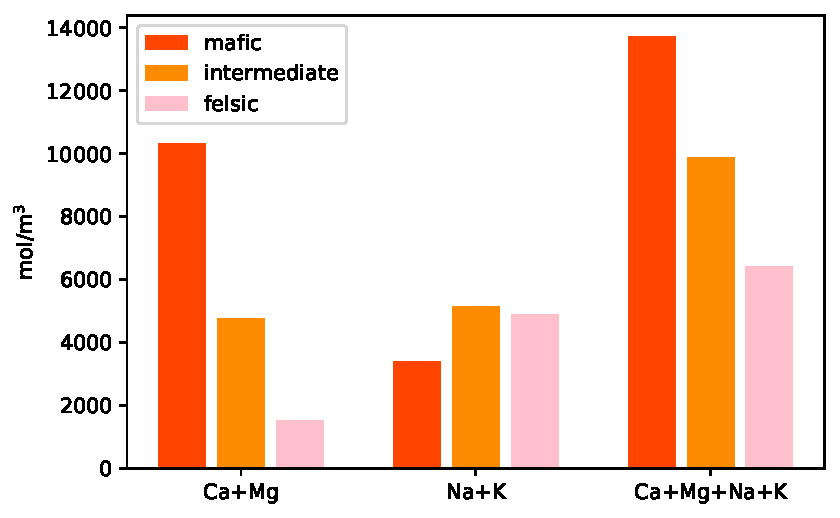
\includegraphics[width=0.6\textwidth]{figures/SEAIs/lithology-composition.pdf}
    \caption[Mean Ca, Mg, Na, and K concentrations within mafic, intermediate, and felsic lithologies.]{Ca, Mg, Na, and K concentrations within mafic, intermediate, and felsic lithologies, as calculated based on the mean of data compiled from EarthChem.}
    \label{fig:lithology-composition}
\end{figure}

A related issue is that our analysis focuses on the weathering of Ca and Mg silicates. Sources of alkalinity to the ocean include the four major cations of Ca, Mg, Na and K. A common approach for the long-term carbon cycle follows that of \citet{Berner1983a} where an emphasis is placed on Ca and Mg with the weathering of Na and K silicates considered to not be a long-term sink of \COtwo. The reasoning behind this assumption is that while weathering of these silicates can lead to transient uptake of \COtwo, this uptake is balanced by release. The ultimate mechanism through which silicate weathering sequesters carbon is the incorporation of Ca+Mg carbonates into the lithosphere. Given that Na and K are not precipitating carbonate, when simulating long term steady-state solutions, as we are here, it is valid to follow the approach of \citet{Berner1983a} and not consider the Na and K cycles. Complexity arises given the long residence time of Na and K in seawater ($\sim$45--80~m.y. for Na, and $\sim$8--10~m.y. for K; \citealp{Emerson2008a, Lecuyer2016a}) and the lag between the generation of alkalinity and its consumption that could modulate the carbonate system. Dynamic modeling of the effects of the Na and K cycles on the long term carbon cycle is an area ripe for future research although uncertainty in their sinks and the timescale of the processes that control them make them difficult to parameterize. An alternative approach for estimating carbon sequestration associated with silicate weathering that sought to incorporate all four cations was taken by \citet{France-Lanord1997a} who used a formulation of $\Delta \textrm{CO}_2 = \Delta \textrm{Mg} + \Delta \textrm{Ca} + 0.15 \Delta \textrm{Na} + 0.1 \Delta \textrm{K}$. This relationship, also applied by \citet{Schopka2011a}, assumes that all Ca$^{2+}$ and Mg$^{2+}$ eventually forms carbonates and applies an estimate that 20\% of K$^{+}$ and 30\% of Na$^{+}$ exchanges for Ca and Mg and ultimately produces carbonate (and considers charge balance). Different parameterizations such as that of \citet{France-Lanord1997a} could modulate our estimates, but the importance of the emergence of the SEAIs on Neogene \pCOtwo would remain unchanged. The relative importance of mafic lithologies also remains given that with significantly higher Ca+Mg concentrations and subequal Na+K concentrations to intermediate/felsic lithologies they have the highest Ca+Mg+Na+K concentrations (Fig. \ref{fig:lithology-composition}).

\section{Climate Model}

For the climate model component of GEOCLIM, we use temperature and runoff fields from a subset of the GFDL CM2.0 experiments (\citealp{Delworth2006a, Delworth2006b}; available for download at \url{https://nomads.gfdl.noaa.gov/dods-data/gfdl_cm2_0/}) These experiments were performed in order to explore the effect of various changes in forcing agents on climate since ca. 1860 at 2.0\degrees $\times$ 2.5\degrees resolution. In the ``1860 control'' experiment, forcing agents representative of conditions ca. 1860 (including \COtwo, CH$_{4}$, N$_{2}$O, O$_{3}$, sulfates, carbon, dust, sea salt, solar irradiance, and the distribution of land cover types) are held constant for 500 years after reaching equilibrium. \pCOtwo in 1860 is assumed to be 286~ppm. In the ``+1\%/yr to 2$\times$'' experiment, initial conditions are taken from the ``1860 control'' experiment, then \pCOtwo is prescribed to increase from 286~ppm at a compounded rate of +1\% per year for 70 years, when \pCOtwo reaches double (572~ppm) of the initial value. \pCOtwo is then held constant until the end of the 280 year experiment. All non-\COtwo forcing agents are held constant. The ``+1\%/yr to 4$\times$'' experiment is identical to the ``+1\%/yr to 2$\times$'' experiment, except that \pCOtwo is prescribed to increase for 140 years, when \pCOtwo reaches quadruple (1144~ppm) of the initial value. \pCOtwo is then held constant for 160 years. We take the mean of the last 100 years of each of these three experiments (when \pCOtwo is being held constant at its final level) to obtain temperature and runoff fields for 286, 572, and 1144~ppm \pCOtwo respectively. Temperature and runoff fields associated with \pCOtwo values between the three modeled \pCOtwo levels (286, 572, and 1144~ppm) are obtained through linear interpolation between the model results.

Given that precipitation in the SEAIs is primarily driven by large-scale convective upwelling leading to high precipitation over both land and water \citep{Donohoe2017a}, the current approach of using a climate model forced by modern paleogeography for all SEAIs scenarios is a reasonable approximation for this region. However, for paleogeographic change that would have very significantly modified precipitation over broad swathes of land such as growth of the Himalaya, this approach of using modern climate model results is not viable. The climate model also assumes the present-day extent of ice-sheets for all \pCOtwo levels. However, without ice-sheets, the global climate would be warmer for a given \pCOtwo (hysteresis loop; \citealp{Pollard2005b}), but the amount of emergent land would be lower. We expect this bias to be minimal, as all of our modeled \pCOtwo estimates fall below the glaciation threshold for Antarctica.

\section{Southeast Asian Islands Scenarios}

\begin{figure}[h!]
    \centering
    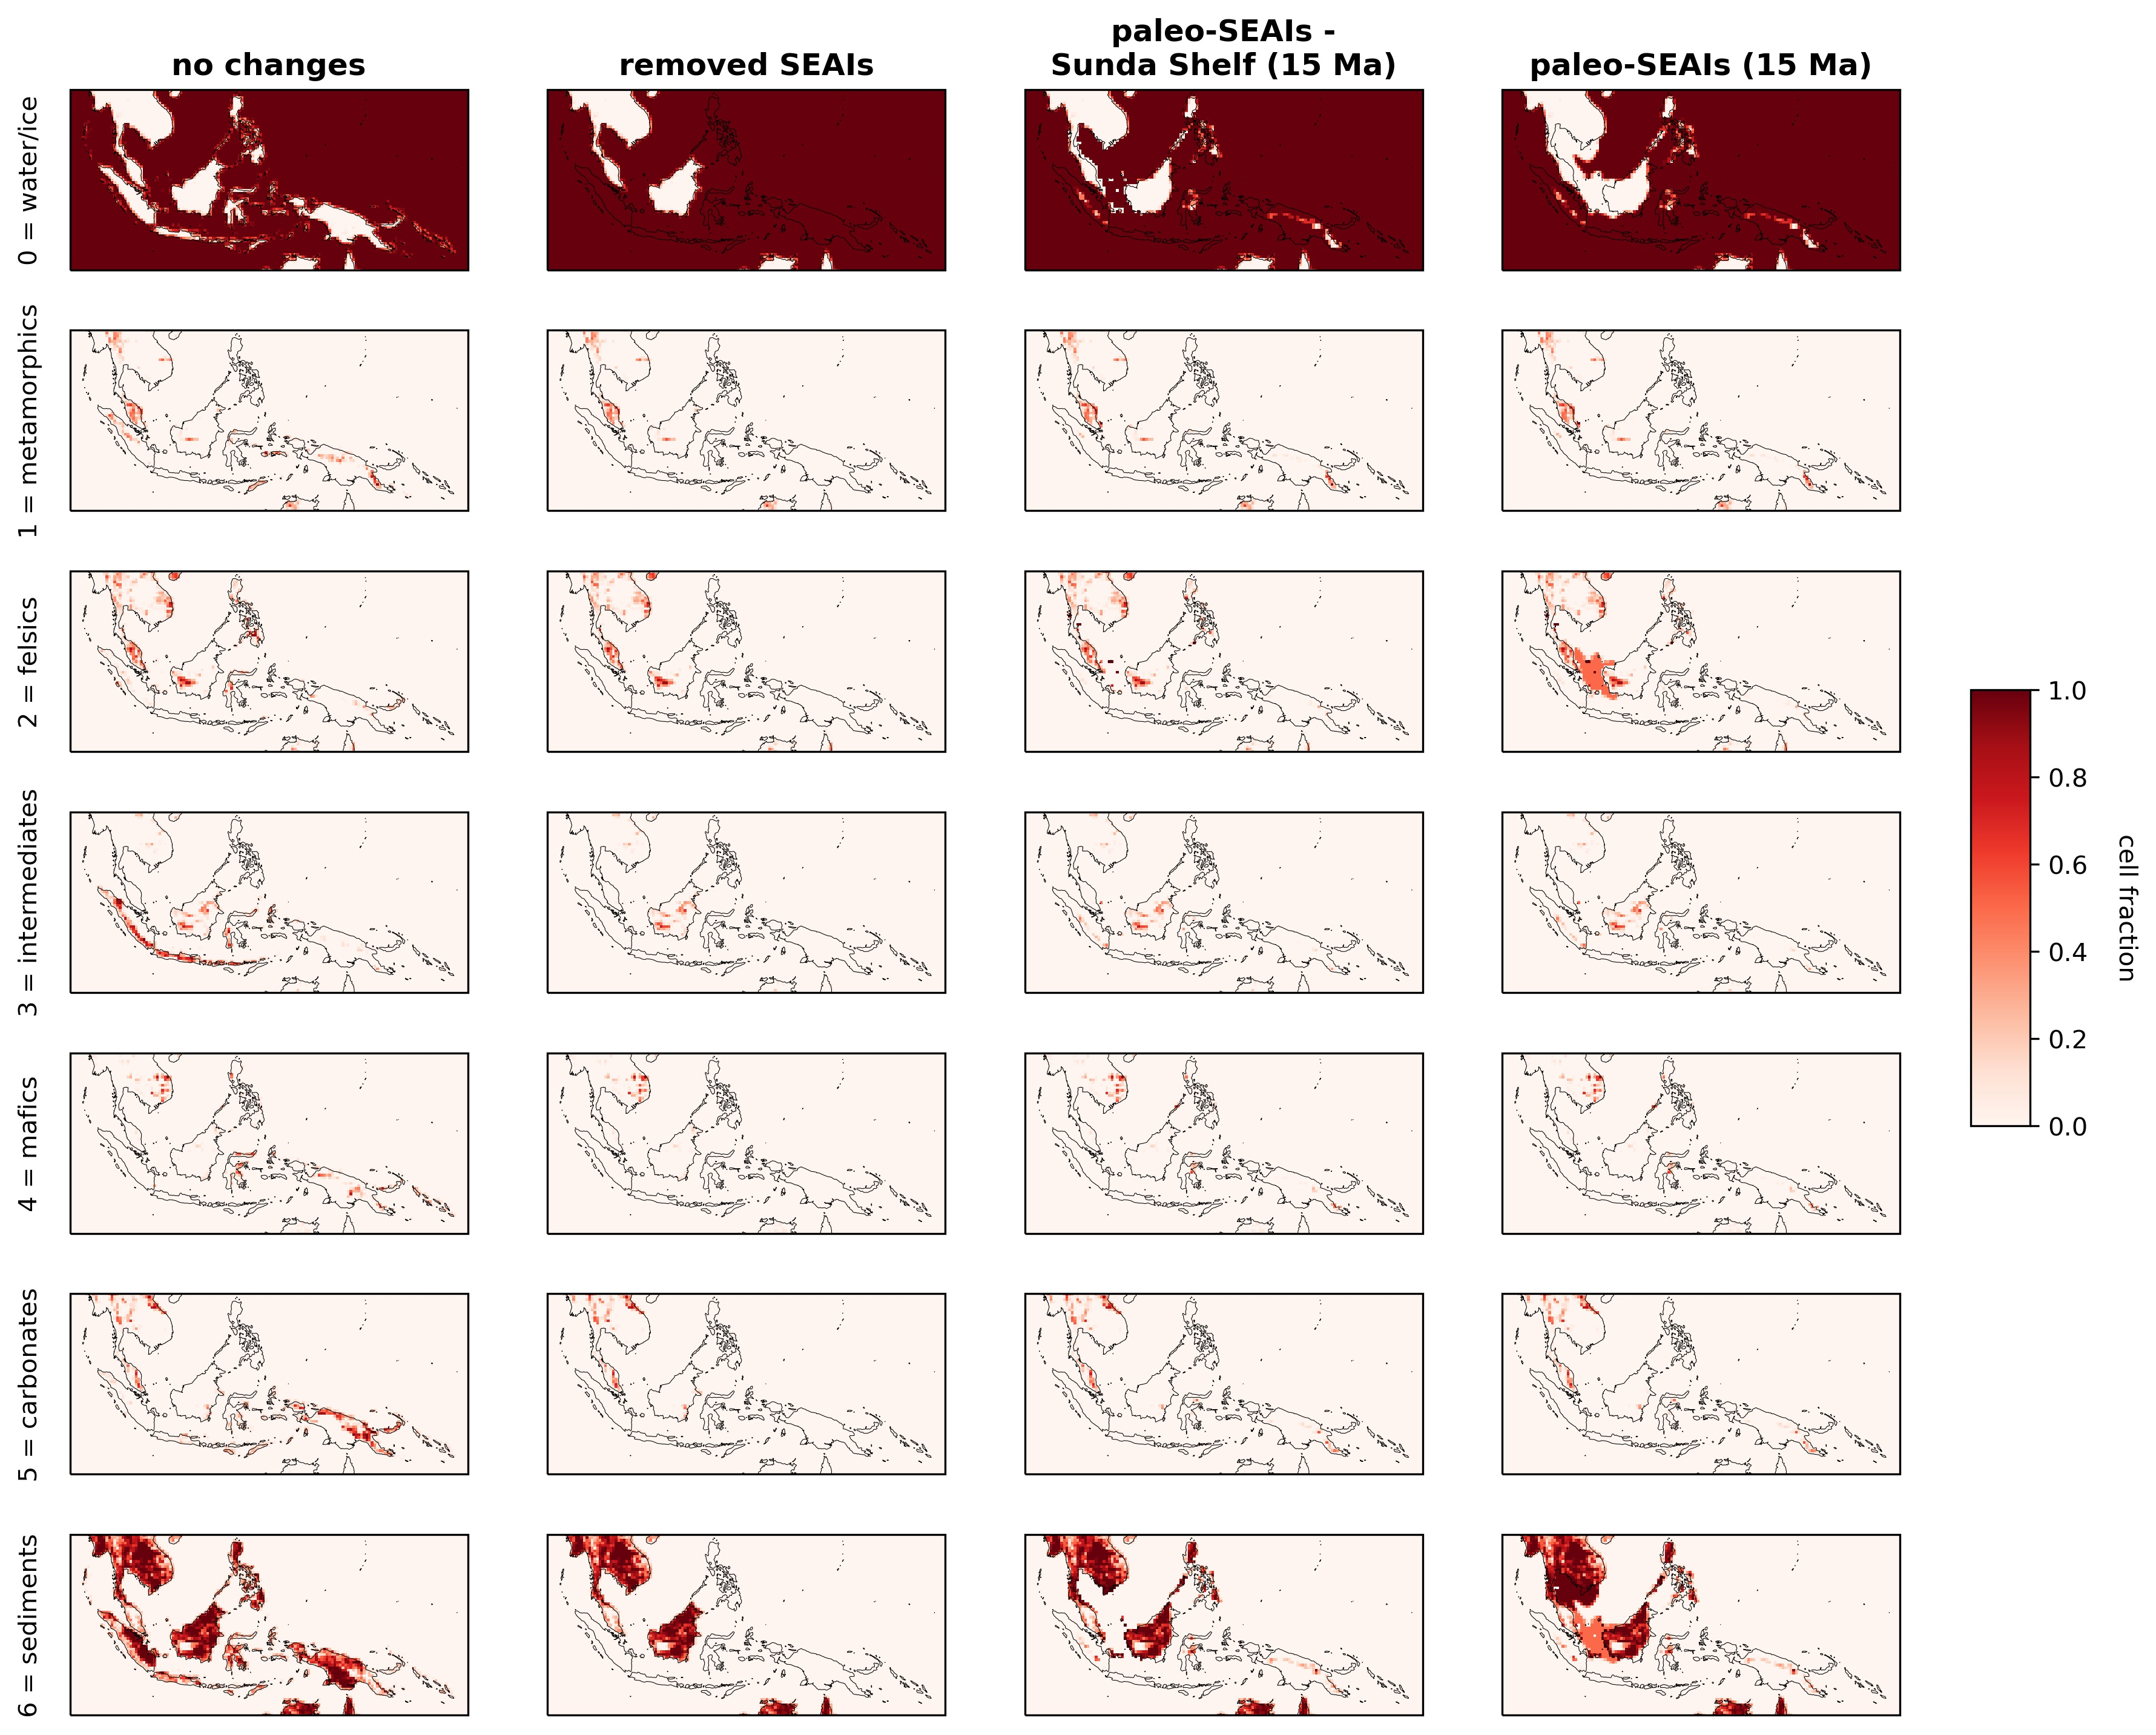
\includegraphics[width=1\textwidth]{figures/SEAIs/SEAI-fracs.jpg}
    \caption[Lithologic maps of the SEAIs used to force GEOCLIM.]{0.5\degrees $\times$ 0.5\degrees lithologic maps of the Southeast Asian islands (SEAIs) used to force GEOCLIM. Only the 15~Ma scenarios are shown here, but the 10 and 5~Ma scenarios would be similar, using the 10 and 5~Ma shorelines shown in Figure 1 of the main text instead. Each column represents a tested scenario. Each row represents a lithologic category. Solid black lines show present-day shorelines. Total areas of each lithologic category within the SEAIs for each of these tested scenarios is shown in Figure \ref{fig:lithology-areas}.}
    \label{fig:SEAI-fracs}
\end{figure}

\begin{figure}[h!]
    \centering
    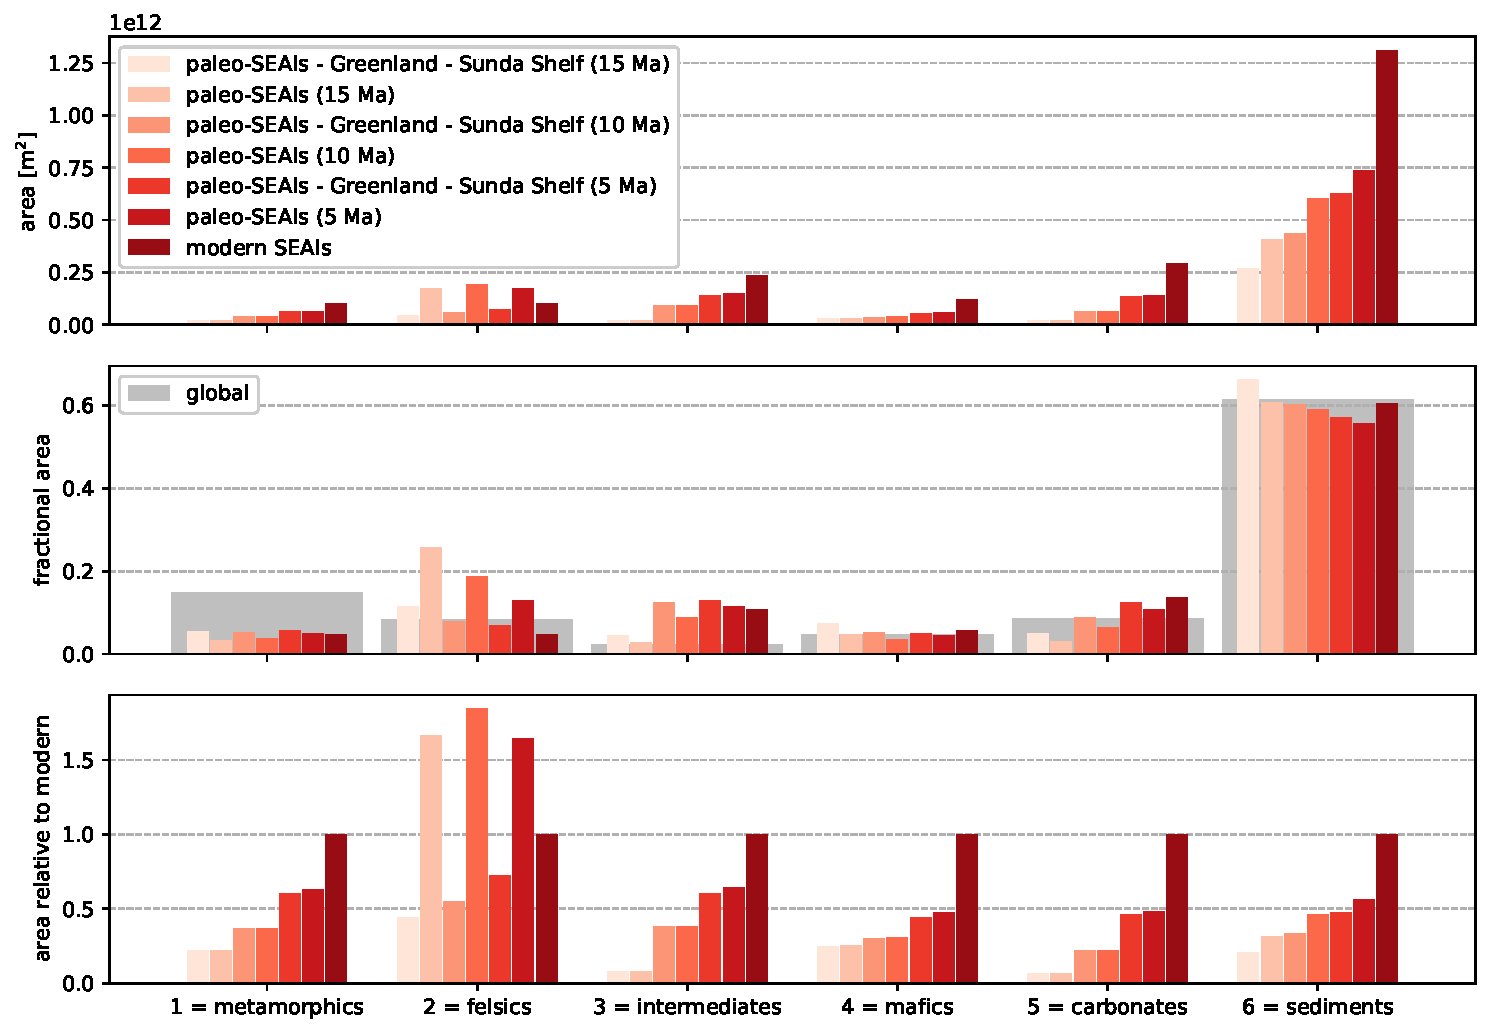
\includegraphics[width=1\textwidth]{figures/SEAIs/lithology-areas.pdf}
    \caption[Total area of the lithologic categories within the SEAIs.]{Total area of the lithologic categories within the SEAIs for each tested scenario. Note that the grey bars in the middle panel indicate the fractional area of each lithologic category for the entire Earth.}
    \label{fig:lithology-areas}
\end{figure}

\begin{figure}[h!]
    \centering
    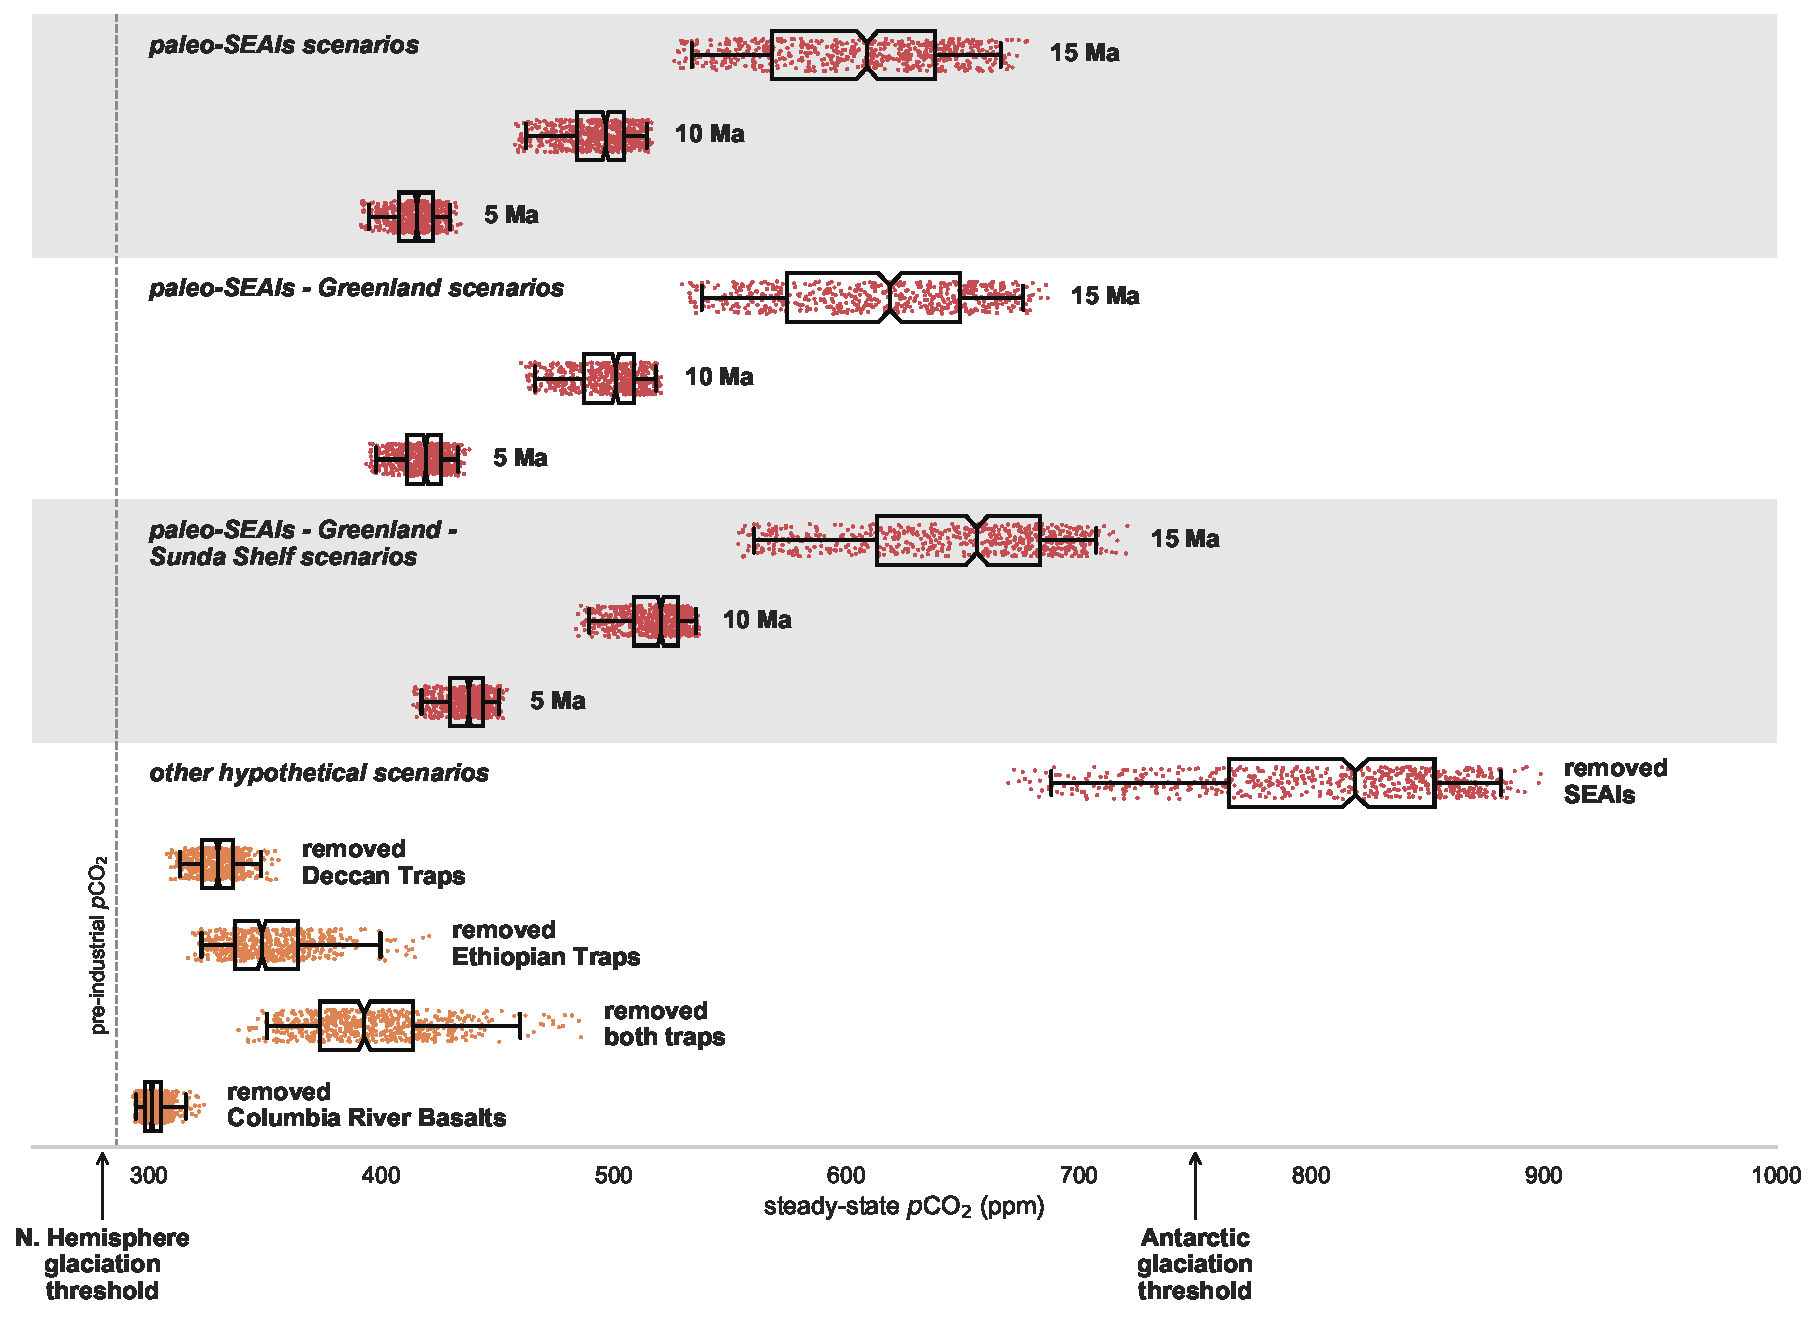
\includegraphics[width=1\textwidth]{figures/SEAIs/scenario-pCO2-all.pdf}
    \caption[Steady-state \pCOtwo estimates from GEOCLIM.]{Steady-state \pCOtwo estimates from GEOCLIM for the various scenarios discussed in the text. For each of the 13 scenarios, each point represents an estimate from one of the 573 unique parameter combinations that resulted in reasonable total global \COtwo consumption and most closely matched estimates of present-day \COtwo consumption in 80 watersheds around the world. The box encloses the middle 50\% of the \pCOtwo estimates (i.e. the interquartile range), and the notch represents the median with its 95\% confidence interval. The whiskers extend to the 2.5 and 97.5 percentile values. This figure is identical to Figure 2 in the main text, except for the addition of the scenarios used to test the sensitivity of the results to the inclusion of the Sunda Shelf and the removal of the Greenland ice sheet.}
    \label{fig:scenario-pCO2-all}
\end{figure}

\begin{figure}[h!]
    \centering
    \includegraphics[width=0.6\textwidth]{figures/SEAIs/paleogeographic-reconstructions.pdf}
    \caption[Paleogeographically reconstructed paleoshorelines for the SEAIs.]{Paleogeographically-reconstructed paleoshorelines for the SEAIs at 5, 10, and 15~Ma, using the paleoshoreline reconstruction of this study coupled to the paleogeographic model of \citet{Matthews2016a}.}
    \label{fig:paleogeographic-reconstructions}
\end{figure}

We use geological data to quantify the changes in the area of the SEAIs over the past 15~m.y. (described in detail in \textit{Paleoshoreline Reconstruction and Geological Synthesis}). To generate the lithologic map used in the ``removed SEAIs'' scenario (Fig. \ref{fig:SEAI-fracs}), we remove all land associated with arc-continent collision in the SEAIs. To generate the lithologic map used in the ``paleo-SEAIs'' scenarios (Fig. \ref{fig:SEAI-fracs}), we take the estimated paleoshorelines of the SEAIs for 15, 10, and 5~Ma, then remove all land that falls outside of these bounds. The slope and lithologic classification of each pixel is identical to that of the present day, provided that these pixels fall within the estimated paleoshorelines of the SEAIs for their respective time slice. This means that while we are changing the amount of emergent land, we are not changing the latitudinal or longitudinal position and are keeping the slope of emerged pixels the same. Given that similar distributions of lithology and slope are reasonable in the past and that latitudinal translation has been relatively minor, we consider this simplification to be reasonable to first-order (Fig. \ref{fig:paleogeographic-reconstructions}). We then add land in the region that is not exposed today. The assignment of lithology, runoff, and slope for pixels on the Sunda Shelf is not trivial, given that the shelf is not currently exposed. As discussed in \textit{Paleoshoreline Reconstruction and Geological Synthesis}, the Sunda Shelf is a flat-lying, relatively stable platform of continental crust. Islands between Malaysia/Sumatra and Borneo are composed of granite and are surrounded by shallow marine siliciclastic sediments \citep{Darmadi2007a, Hall2009a, Hall2013b}. However, basement highs of granite do not appear further to the northwest in the Gulf of Thailand, and seismic and drill core data suggest siliciclastic fluvial systems draining out toward the South China Sea when the Sunda Shelf was exposed \citep{Darmadi2007a}. We therefore assign pixels of the Sunda Shelf between Malaysia/Sumatra and Borneo to be 50\% felsic and 50\% sediment, and pixels further to the north to be 100\% sediment. For the slope, we take the mean slope value (0.0043~m/m) of relatively flat land on eastern Sumatra, and assign this value to all pixels of the Sunda Shelf. For the runoff, we linearly interpolate along latitude bands between present-day land pixels to obtain runoff values for the presently-submerged Sunda Shelf. This approach preserves large N-S variation in runoff associated with the large-scale Hadley circulation and therefore should be reasonable to first-order, although it does not accurately capture the smaller-scale interactions between land and ocean/atmosphere circulation. For other minor islands in the region that were exposed 15, 10, or 5~m.y. ago, but are currently submerged, we take the same approach as that described for the Sunda Shelf to generate the runoff field. For the slope and lithology, we take the mean slope and Ca+Mg concentrations from neighbouring pixels. We also remove the Greenland ice sheet in the ``paleo-SEAIs'' scenarios, to be consistent with Northern Hemisphere ice sheets developing after 5~Ma \citep{Haug2005a}. The runoff field over Greenland is generated using the same method as that for the Sunda Shelf. For the slope, we take the mean slope value (0.0529~m/m) of land for which slope data exists around the edges of Greenland, and assign this value to all pixels of Greenland covered by the ice sheet. We also assign the Ca+Mg concentration of bulk continental crust to these pixels.

To explore the sensitivity of our results to the inclusion of the Sunda Shelf and the removal of the Greenland ice sheet, we also tested ``paleo-SEAIs - Greenland'' scenarios for 15, 10, and 5~Ma, which are identical to that of the ``paleo-SEAIs'' scenarios without the removal of the Greenland ice sheet. We also tested ``paleo-SEAIs - Greenland - Sunda Shelf'' scenarios for 15, 10, and 5~Ma, which are identical to that of the ``paleo-SEAIs'' scenarios without the inclusion of the Sunda Shelf and the removal of the Greenland ice sheet. We find that the estimated steady state \pCOtwo's for the ``paleo-SEAIs - Greenland'' and ``paleo-SEAIs - Greenland - Sunda Shelf'' scenarios are only marginally higher than those of the ``paleo-SEAIs'' scenarios (Fig. \ref{fig:scenario-pCO2-all}), suggesting that our results are relatively insensitive to the inclusion of the Sunda Shelf and the removal of the Greenland ice sheet. This insensitivity can be attributed to the low Ca+Mg concentrations of felsic and sediment lithologies in conjunction with the low relief across the Sunda Shelf, and the low runoff values at high latitudes.

\begin{figure}[h!]
    \centering
    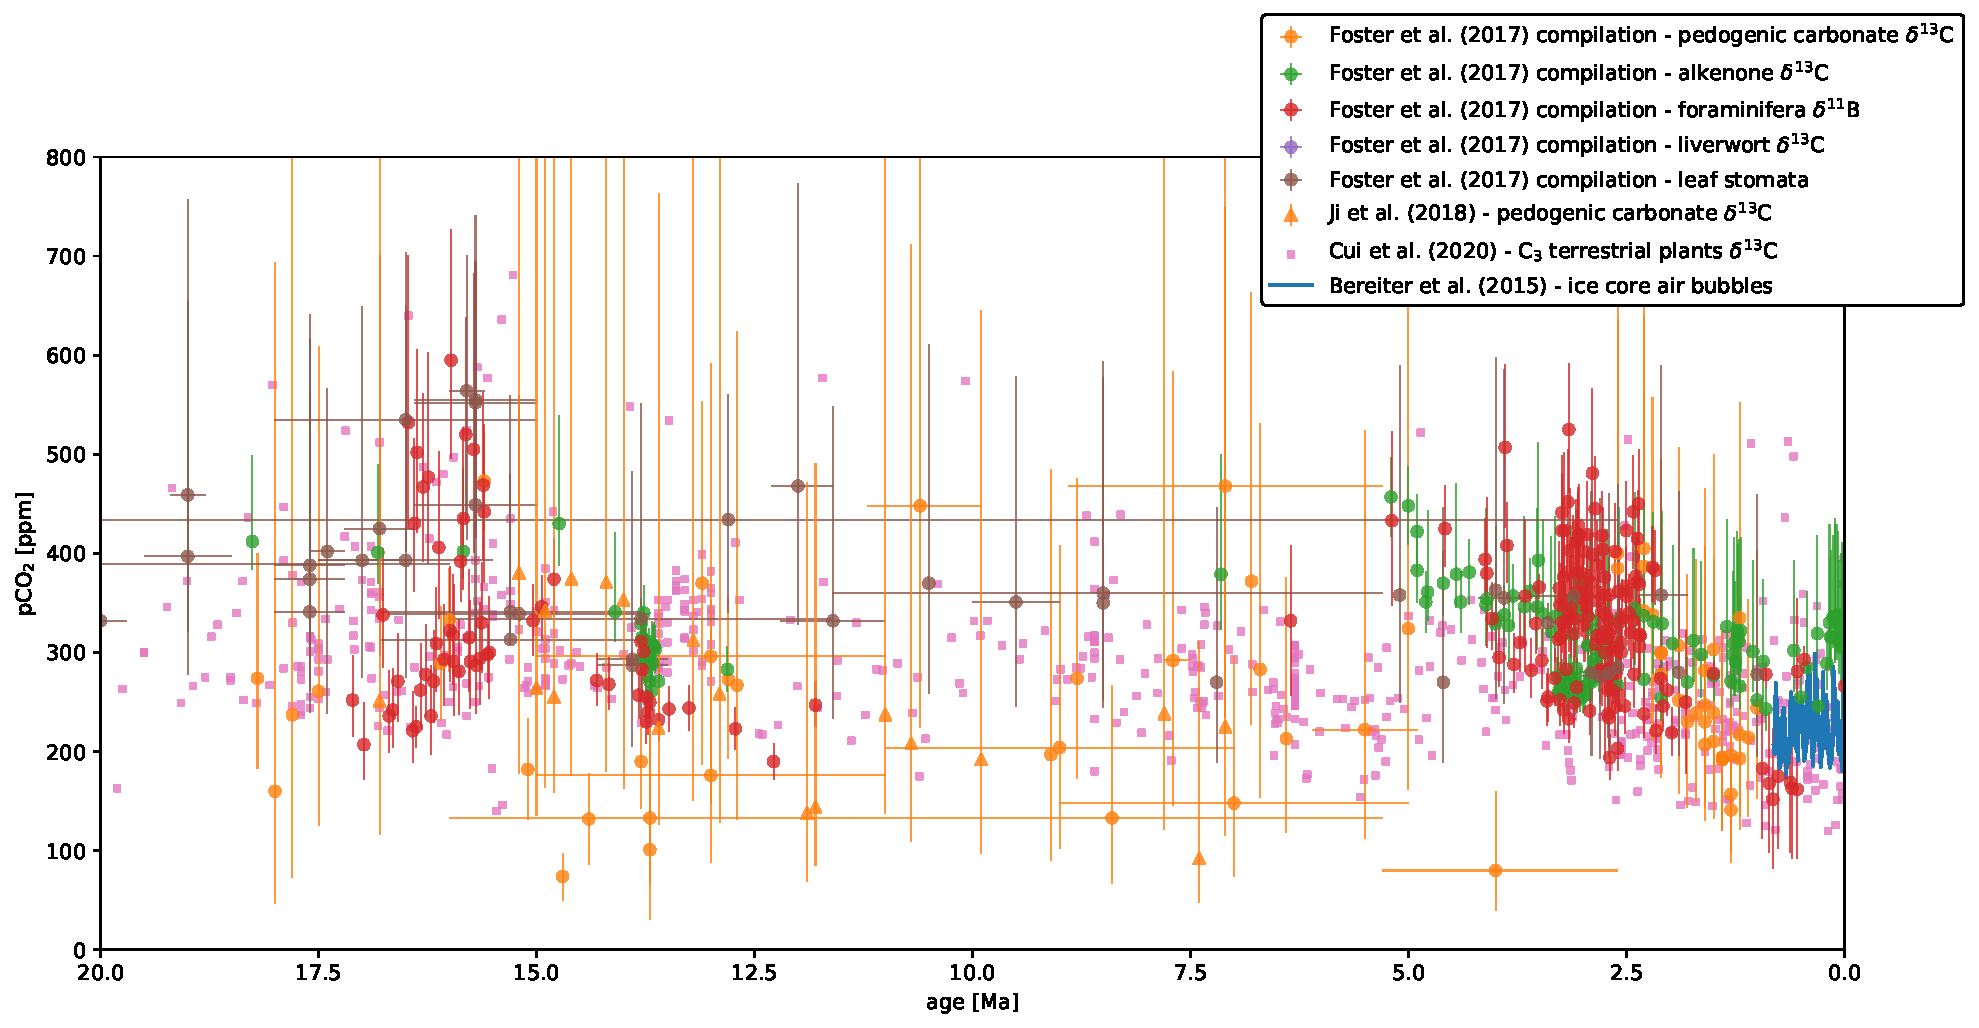
\includegraphics[width=1\textwidth]{figures/SEAIs/pCO2-proxies.pdf}
    \caption[Proxy-based \pCOtwo estimates for the past 20~m.y.]{Proxy-based \pCOtwo estimates for the past 20~m.y. For data that were compiled within \citet{Foster2017a}, error bars indicate standardized uncertainties. For the \citet{Ji2018a} data, error bars represent the 16-84$^{th}$ percentile of resampled estimates. Individual data points from \citet{Cui2020a} were not published with uncertainties. The \citet{Bereiter2015a} data come from the EPICA Dome C ice core.}
    \label{fig:pCO2-proxies}
\end{figure}

Proxy-based \pCOtwo estimates for the past 20~m.y. are shown in Figure \ref{fig:pCO2-proxies} \citep{Bereiter2015a, Foster2017a, Ji2018a, Cui2020a}. Even when stringent quality criteria and the latest understanding of each of the \pCOtwo proxies have been applied to available \pCOtwo records, both significant uncertainty in the estimated \pCOtwo for any given data point as well as disagreement between techniques remain. Statistical methods that are often utilized in an attempt to extract trends from this data (e.g. locally-weighted scatter plot smoothing, LOWESS) evaluate the mean (with some weighting) of the highly scattered data in a given time interval. However, such methods are only appropriate for estimating the ``true'' value at any given time interval in datasets in which individual data points are being drawn from a single distribution about a mean value. The \pCOtwo proxy compilation shown in Figure \ref{fig:pCO2-proxies} consists of several distinct techniques and samples, each with their own set of assumptions and associated probability distributions that influence their reported values. Therefore, running a regression through these values neglects the fact that some of these techniques/samples are likely more reliable than the others. Constraining how robust each \pCOtwo proxy technique is remains an important challenge, and as such the ``true'' \pCOtwo could plausibly lie anywhere within the full range of proxy-based \pCOtwo estimates for any given time interval. Nevertheless, our modeled \pCOtwo values for 15~Ma (Fig. \ref{fig:scenario-pCO2-all}) resemble the higher end of proxy-based \pCOtwo estimates for the early-mid-Miocene. Given this scatter in the proxy-based \pCOtwo estimates, we instead infer the Neogene cooling trend from the Miocene benthic foram oxygen isotope record shown in Figure 1 in the main text.

\section{Paleoshoreline Reconstruction and Geological Synthesis}

Geological maps, stratigraphic data, and previous paleoshoreline compilations were used to calculate the changes in different types of subaerially exposed rocks in the SEAIs. Following \citet{Molnar2015a}, we analyzed the area changes of islands that are larger than $\sim$200~km$^{2}$ (Fig. 1 in main text). We also included changes in areas of submerged continental shelves that were previously exposed, like the Sunda Shelf. Larger islands were further divided into regions based upon their position on microplates as defined by \citet{Matthews2016a}. Miocene to present stratigraphic columns were compiled from each region to develop an age model for paleoenvironmental indicators. In general, carbonate strata and thin-bedded siliciclastic strata were assumed to be deposited in a subaqueous marine environment, whereas evidence for exposure and terrestrial siliciclastic deposits were used as indicators of a subaerial paleoenvironment. Following previous paleoshoreline compilations and these environmental indicators, paleoshorelines were outlined in QGIS to calculate areas for the Early Pliocene (5 Ma), Late Miocene (10 Ma), and Middle Miocene (15 Ma). The paleoshoreline reconstructions within the paleogeographic models broadly coincide with sub-Epoch boundaries (i.e. Early Miocene = 23--16~Ma, Middle Miocene = 15.99--11.61~Ma, Late Miocene = 11.6--5.4~Ma, Pliocene =5.39--3.8 Ma), but we recognize that the biostratigraphic resolution is an additional source of uncertainty.

Several new sources for paleoshoreline data have become available since \citet{Molnar2015a}. Particularly, for Sulawesi, we follow the recent stratigraphic compilation and paleoshorelines delineated by \citet{Nugraha2018a}, and in New Guinea, we follow \citet{Gold2017a} and \citet{Harrington2017a}. Although the outlines of our paleoshorelines are significantly different from those used for 5~Ma by \citet{Molnar2015a} our calculated area is comparable.

\subsection{Malay Peninsula and Sunda Shelf}

Paleogeographic reconstructions of Peninsular Malaysia suggest that it has been largely exposed over the last 20~Ma \citep{Hall2002a, Hall2013b}. Although the majority of the Sunda Shelf is currently submerged, large portions of this flat-lying, relatively stable platform of continental crust were also emergent throughout the Neogene, and were repeatedly subaerially exposed during the Pleistocene as recently as the Last Glacial Maximum \citep{Hall2002a}. Similarities between the terrestrial biotas of Borneo and mainland Southeast Asia confirm the existence of land bridges on the Sunda Shelf throughout the Miocene \citep{Moss1998a}. Eocene through Miocene rifting of the South China Sea resulted in subsidence throughout the Sunda Shelf \citep{Morley2013a}. Grabens associated with this subsidence became freshwater rift lakes that later transitioned to partially enclosed inland seas and extensive brackish or saline wetland environments. Palynological analysis suggests widespread swamp environments persisting through the Late Miocene \citep{Morley2013a}. Basement highs (e.g. the Natuna Arch, currently subaerially exposed as the largely granitic island of Natuna off SW Borneo, as well as the granitic Tin Islands south of the Malay Peninsula) are typically bounded by Paleogene to Neogene basins dominated by shallow marine clastic fill \citep{Darmadi2007a}. Most paleogeographic reconstructions of the region incorporate some degree of exposure of the Sunda Shelf from 20~Ma onwards \citep{Hall2013b, Madon2013a}, although it is omitted in the 5~Ma paleogeographic model of \citet{Molnar2015a}.

\subsection{Borneo and Palawan}

Our reconstructions of the paleoshorelines of Borneo and Palawan are largely informed by extant paleogeographic constructions detailed in \citet{Hall2001a, Hall2013a, Hall2013b}, as well as geologic maps and local shoreline reconstructions found in \citet{vandeWeerd1992a, Witts2012a, Madon2013a, Kessler2015a}. Comprised of Paleozoic to Mesozoic crustal components that were largely accreted to Sundaland by the late Cretaceous \citep{Metcalfe2013a}, the southern and western portions of Borneo (SW Kalimantan) have been subaerially exposed throughout the Neogene \citep{Hall2013a, Hall2013b}. A collision along the northern margin of Borneo associated with the initiation of rifting in the South China Sea resulted in the late Eocene uplift of the Central Range mountains \citep{Hutchison1996a}, which provide sediment to basins along the Southern (Kalimantan) and northern (Sabah and Sarawak) coasts of the island. In the east, the Barito, Kutei, and Tarakan basins developed as a single area of subsidence (associated with the opening of the Makassar Straits in the Eocene) before the basins were isolated by Oligocene faulting and Miocene uplift \citep{Witts2012a}. The Kutei Basin is characterized by eastward-prograding deltaic and shallow shelf deposits that have been steadily supplied with sediment from the Schwaner Mountains of SW Kalimantan and the Central Range \citep{vandeWeerd1992a}. North of the Kutei Basin, the deltaic deposits found in the Tarakan Basin similarly prograde eastward from the mid Miocene onward, fed by the northern drainages of the Central Range \citep{Satyana1999a}. In SE Kalimantan, the Barito Basin is bounded to the east by the ophiolite-bearing Meratus Mountains. Sedimentological data suggests that the Meratus Mountains were not emergent until the Late Miocene \citep{Witts2012a}.

Separated from the Paleozoic continental core of SW Borneo by the Lupar Line suture zone, the northern portion of Borneo (Sabah) is underlain by ophiolitic basement that extends to Palawan \citep{Hall2008a, Ilao2018a}. The Sarawak Basin and NW Borneo trough offshore Sabah host $>$10~km-thick Neogene sedimentary sequences, indicative of the extent and duration of exhumation in northern Borneo \citep{Hall2008a}. The Late Oligocene/Early Miocene Sabah Orogeny resulted in the uplift of both Sabah and southern Palawan \citep{Hall2013a}, as well as the obduction of the Palawan ophiolite and Telupid ophiolite of northern Sabah. Under-thrusting of thinned passive-margin continental crust beneath these suprasubduction ophiolites resulted in Early to Middle Miocene exhumation and offshore unconformities \citep{Hall2008a}. Early Miocene sediments in northern Sabah have a provenance from Palawan \citep{Suggate2014a}, indicating that Palawan, like northern Borneo, experienced uplift during the Sabah orogeny. However, initiation of back-arc extension in the Sulu Sea around 19~Ma \citep{Hall2013a} resulted in the subsidence of the eastern Palawan Mountains, eliminating or reducing the role of Palawan as a sediment source for the Borneo trough. The 14~Ma Capoas Granite on Palawan and the 7.5~Ma Kinabalu Granite in Sabah are interpreted to be the result of crustal thinning related to pulses of regional backarc extension \citep{Hall2013a}. Thermochronological data from the Sabah highlands suggest extremely rapid uplift (7~km/m.y.) and exhumation during the latest Miocene and early Pliocene, resulting in the recent formation of Mt. Kinabalu, the tallest peak in Borneo \citep{Cottam2013a}.

\subsection{Sulawesi}

For the paleoshorelines of Sulawesi, we largely followed the recent stratigraphic compilation and paleoshorelines compilation of \citet{Nugraha2018a}. Geographically, Sulawesi can be divided into a central highland region flanked by North, South, Southeast, and East Arms. These arms have high relief ($>$3~km) that are separated by deep basins and broadly define Sulawesi's seven tectonic provinces: 1) the West Sulawesi magmatic arc of the South Arm, 2) the Central Sulawesi metamorphic Belt, 3) the Sangihe arc of the North Arm, 4) the East Sulawesi Ophiolite of the East Arm, 5) the southeast metamorphic belt of the Southeast Arm, and the microcontinental blocks of 6) Banggai-Sula and 7) Buton-Tukang Besi \citep{Hamilton1979a, Katili1978a}. Like SW Borneo, the North and South Arms, and much of Central Sulawesi, are underlain by continental blocks that rifted off of the Australian-Birds Head margin in the Jurassic and collided in the Cretaceous with Eurasian basement of Sundaland as part of the Woyla Arc system \citep{Parkinson1998b, Hennig2016a, Hall2017a, Hennig2017a}. After collision, subduction polarity reversed and a Cretaceous to Miocene SE-facing volcanic arc developed \citep{Polve1997a, Elburg1998a} that was connected to the paleo-Sunda Arc \citep{Hall2002b}, also referred to as the Great Indonesian arc \citep{Harris2006a}.  The ophiolites of Sulawesi were generated in this arc system in a back-arc to intra-arc setting \citep{Monnier1995a} (but see \citealp{Kadarusman2004a} for an alternative view) and the largest fragments of the East Sulawesi ophiolite were detached from their metamorphic sole in the late Oligocene (32--28~Ma; \citealp{Parkinson1998a}) and thrust to the east above a west dipping slab (East Sulawesi block; \citealp{Villeneuve2001a}). During the Early to Middle Miocene, the Tukang Besi-Buton block began to collide obliquely with the southeastern end of the Sunda Arc, causing ophiolite emplacement in West and SE Sulawesi, including Buton \citep{Smith1991a, Bergman1996a}.

The North Arm consists of Late Pliocene and younger volcanic rocks built upon Eocene to Early Miocene oceanic basalt, basaltic andesite, pelagic sediments, and metamorphic rocks \citep{Elburg1998a}. Eocene to Early Miocene volcanic rocks formed above a NW dipping slab in an arc system that extended to West and South Sulawesi \citep{vanLeeuwen2005a}. Gorontalo Bay is an extensional basin that formed in the Pliocene, and prior to that time, the East Sulawesi was attached to the North Arm of Sulawesi. After the Oligocene to Early Miocene accretion of the East Sulawesi ophiolite, the arc system stepped out to the SE forming a Neogene (23--16~Ma) volcanic belt on the East arm \citep{Kadarusman2004a}. In the Late Miocene, SE-dipping subduction was initiated below the North Arm, which continues today at the North Sulawesi Trough. North Sulawesi was not substantially emergent until the Pliocene \citep{vanLeeuwen2005a}. Active volcanoes extend from the North Arm through the Sangihe Arc into the southern Philippines.

The East and Southeast Arms consist predominantly of mafic and ultramafic rocks of the East Sulawesi Ophoilite that are exposed for more than 10,000~km$^{2}$ \citep{Monnier1995a}. The East Arm preserves a complete ophiolitic sequence underlain by a metamorphic sole, m\'elange, imbricate continental margin and crystalline basement with a blueschist metamorphic overprint \citep{Silver1983a, Monnier1995a, Parkinson1998a}. Locally, the structural thickness of the ophiolite exceeds 15~km with surface relief over 3~km \citep{Kadarusman2004a}. Seventeen igneous K-Ar dates from the East Sulawesi ophiolite range from 93--32~Ma, clustering between 60~Ma and 40~Ma \citep{Parkinson1998b}. K-Ar dates on hornblende from the metamorphic sole yielded cooling ages between 36--23~Ma \citep{Parkinson1998a, Villeneuve2001a}, which dates the initial emplacement of the East Sulawesi ophiolite as the north Sulawesi volcanic arc was underthrusted by the Sula spur (Australian crust) \citep{Silver1983a, Parkinson1998a}; however, despite these relatively old ages of emplacement, it appears that the ophiolites on the East Arm were not substantially subaerially exposed and exhumed until the Miocene.

Collision of the Sula-Banggai block with the East margin of Sulawesi began in the latest Miocene and uplift accelerated in the early Pliocene (5.2~Ma to 3.8~Ma) and is associated with a major pulse of sedimentation in adjacent basins \citep{Davies1990a, Villeneuve2000a}. Off the northeast margin of the east arm of Sulawesi, Miocene platform carbonates on the Sula-Banggai block are overlain by Late Miocene to Early Pliocene ophiolite detritus in the Celebes m\'elange \citep{Davies1990a}. Thus, although the East Sulawesi ophiolite was trapped/emplaced onto the composite Sundaland margin (i.e. a fragment of previously accreted Australian crust) between 36~Ma and 23~Ma, mafic and ultramafic rocks on the south and west arms appear to have not been substantially subaerially exposed in the south and west arms until after 15~Ma, and on the east arm until after 5~Ma.

West Sulawesi rifted from Borneo during the Eocene forming the Makassar Straits back arc basin behind a southwest-facing arc \citep{Polve1997a}. Eroded fragments of ophiolite and extensive belts of volcanic rocks are preserved on the West and South Arms of Sulawesi \citep{Bergman1996a, vanLeeuwen2010a}. During the Middle Miocene (ca. 15--13~Ma), extensional faults in the Bone basin reversed, which was accompanied by uplift and erosion of the Bone Mountain ophiolite and Lamasi complex in West Sulawesi \citep{Bergman1996a, vanLeeuwen2010a}. Shortening was likely due to the collision of the leading edge of the Buton-Tukang Besi block, which collided with Buton and the SE Arm of Sulawesi \citep{Smith1991a}. Uplift and erosion is recorded by the presence of a major Middle Miocene unconformity and sedimentary breccias in marginal basins \citep{Bergman1996a, vanLeeuwen2010a}. Uplift was diachronous, not effecting units below and to the west of the Lamasai ophiolite until the Middle Miocene (ca. 13~Ma) \citep{vanLeeuwen2010a}. Alkali volcanism ensued at ca. 11~Ma and is associated with a second phase of extension and exhumation from the Late Miocene to Pliocene with fission track ages implying deep exhumation \citep{Smith1991a, Bergman1996a, vanLeeuwen2010a}.

Fission track ages from granitoids in central Sulawesi indicate rapid uplift of Central Sulawesi (200--700~m/m.y.) starting at about 5~Ma associated with movement on the Palo-Koro fault \citep{Bellier2006a}. The fault system also shows a normal component with rapid exhumation of rock west of the fault in western Sulawesi -- all fission track dates are younger than 5~Ma \citep{Bellier2006a}. Just east of the Palo-Koro fault, the Palu Metamorphic Complex was exhumed in the Late Miocene to early Pliocene in the north (ca. 5.3~Ma) and later Pliocene in the south (ca. 3.1--2.7~Ma) at rates of up to 400~m/m.y. \citep{Hennig2017b}.

\subsection{New Guinea and Halmahera}

Paleoshoreline maps were georeferenced from several previous tectonic and paleogeographic analyses, most notably those of \citet{Nichols1991a, Cloos2005a, Gold2017a, Harrington2017a}. These studies were all based to varying degrees on lithological distributions, biostratigraphic, borehole data, and tectonic models. We complimented these data with our stratigraphic compilations for the region to provide further paleoenvironmental context.

Northern New Guinea, including the Melanesian Arc, was emplaced above the Australian plate during the Miocene \citep{Hamilton1979a, Cloos2005a, vanUfford2005a, Baldwin2012a}. Two major ophiolite belts marking the suture -- the Irian-Marum ophiolite belt (including the April ultramafics), and the Papuan Ultramafic Belt (PUB) -- are preserved along the Central Range and Peninsular Range, respectively. South of the Irian-Marum ophiolites, the Ruffaer Metamorphic Complex constructed from the accretionary wedge, forms the spine of the Central Range (up to $\sim$5~km elevation today).

The Middle Miocene (16--14~Ma) basal Makats Formation contains siliciclastic sediment that was transported from the south into the forearc basin associated with the Irian-Marum ophiolite belt \citep{Visser1962a, Cloos2005a}. The beginning of widespread synorogenic sedimentation to the south and on the Australian continental basement was later at ca. 12~Ma \citep{vanUfford2005a}. Mountain building began in Late Miocene time, ca. 8--7~Ma \citep{vanUfford2005a, Baldwin2012a}, but major relief was not generated until the Pliocene \citep{Weiland1996a}. Similarly, the Marum ophiolite was uplifted between 8--5~Ma with 3--4~km of denudation \citep{Crowhurst1996a}. An estimated 80--100~km of shortening has been accommodated by deformation on the south side of the Central Range \citep{Hill1989a, Cloos2005a}.

Along the Papuan Peninsula of Eastern New Guinea, the PUB was obducted above a north dipping slab during Oligocene arc-continent collision between Australian continental fragments and the Melanesian arc, but remained largely subaqueous until the Miocene \citep{Davies1971a, Davies1984a, vanUfford2005a}. Miocene to present arc-continent collision in New Guinea has progressed from west to east. Exhumation of the Central Range accelerated over the past 4~m.y. which is interpreted to be the result of slab-breakoff and buoyant uplift \citep{Cloos2005a}. A change to left-lateral lateral motion on the northern coast of New Guinea at this time, caused the exhumation of ophiolites both along the coast \citep{Monnier1999a} and on the islands Obi \citep{Ali2001a} and Halmahera \citep{Hall1988a, Ballantyne1992a}. In eastern New Guinea, progressive jamming of the north-dipping subduction zone has caused major uplift over the past 4~Ma \citep{vanUfford2005a}, which is well dated with a change in provenance from continental to volcanic detritus \citep{Abbott1994a} and thermochronology \citep{Hill1989a}.

In the Bird’s Neck of western New Guinea, the Lengguru fold belt formed during Middle to Late Miocene clockwise rotation and obduction of the Weyland Terrane \citep{Bailly2009a}. Recent counter-clockwise rotation has exhumed several core complexes and has produced Pliocene compressional deformation to the southwest in the Misool-Onin-Kumawa Ridge \citep{Sapin2009a}.

\subsection{Philippines}

Our reconstructions of the paleoshorelines of the Phillipines were primarily informed by the paleogeographic reconstructions of \citet{Hall1997a}, coupled with geologic maps of the archipelago \citep{GeologicalSurveyDivision1963a}. The Philippine ophiolites have been grouped in four distinct belts \citep{Yumul2007a}. We combine belts 1 and 2 in an eastern suture zone and belts 3 and 4 in a western suture zone. Belts 1 and 2 were juxtaposed in the eastern suture zone during sinistral transpression, which resulted in Early Miocene uplift and deposition of coarse clastic sediments \citep{Pubellier1991a}. The Palawan microcontinental block and Philippine mobile belt collided during late Early Miocene to early Middle Miocene resulting into the emplacement of the western ophiolites, with exhumation extending from the Late Miocene to the present \citep{Yumul2013a}. In addition to collision, arc magmatism contributed significantly to crustal growth in the Philippines \citep{Dimalanta2006a}.

\subsection{Sunda-Banda Arc}

Paleoshoreline reconstructions of the Sunda-Banda Arc system relied largely on the work of \citet{Hall2013a}. The Sunda-Banda Arc system is composed of thick sequences of mixed sedimentary rocks and basement intruded and overlain by igneous rocks derived from continual arc magmatism through much of the Cenozoic \citep{Hall2017a}. Sumatra is the largest island within the Sunda-Banda Arc system that stretches from the Andaman Sea in the northwest to the Banda Sea in the east. The western portion of the Sumatra is underlain by the Wolya ophiolite, which was obducted in the Cretaceous and exhumed in the Eocene to Oligocene \citep{Allen2008a}, whereas the southeast corner on the islands of Bangka and Belitung is composed of granite basement of the Sunda Shelf \citep{Hall2009a, Hall2013b}. Java is composed of a complex of E-W-striking deformational and magmatic belts \citep{AudleyCharles2004a}. The belts have a volcanic arc in the south and a continental shelf to the north with an adjacent sedimentary basin \citep{AudleyCharles2004a}. Bali and Flores are mostly volcanic with some sedimentary cover \citep{Hall2009a}.

Exhumation of the modern Sunda-Banda Arc is the result of ongoing arc-continent collision with the subducting Australian Plate \citep{Harris2006a}. From ca. 20--10~Ma, the majority of Sumatra and nearly all of Java were submerged, although Bangka and Belitung were exposed in addition to a portion of the greater Sunda Shelf \citep{Hall2009a, Hall2013b}. Six major islands were subaerially exposed before 5~Ma: Sumatra, Belitung, Bangka, Java, Bali, and Flores. However, most of Sumatra and Java were elevated above sea level and emerged to their present exposures only since 5~Ma \citep{Hall2009a, Hall2013b}. Most of the non-volcanic islands of the Outer Banda Arc emerged after 5~Ma, associated with slab roll-back and collision with the Australian continental margin \citep{AudleyCharles2004a, Harris2006a, Hall2013b}. In Timor and Sumba, arc-continent collision resulted in rapid uplift of deep marine sedimentary rocks to elevations $>$1~km above sea level with estimated average uplift rates of 1.5~km/m.y. \citep{AudleyCharles1986a}.
\chapter[Supporting Information for ``The lead-up to the Sturtian Snowball Earth: Neoproterozoic chemostratigraphy time-calibrated by the Tambien Group of Ethiopia''][Supporting Information - Tambien Group]{Supporting Information for ``The lead-up to the Sturtian Snowball Earth: Neoproterozoic chemostratigraphy time-calibrated by the Tambien Group of Ethiopia''}

This document accompanies the discussion contained in the main text. All the Python code used for this study, as well as the associated data tables not included in this document, can be found at \url{https://github.com/Swanson-Hysell-Group/2019_Tambien_Group}. A release of this GitHub repository was also made and published at \url{https://doi.org/10.5281/zenodo.3403180}.

\section{Construction of the Chemostratigraphic Composite}

The main text contains a composite \dC and \SrSr curves for the Tonian and Cryogenian that are time-calibrated by the record from Ethiopia and incorporate data from the literature from numerous sources. Additional details associated with the data sets within this composite are provided below. The Python code used to develop the composite as well as the associated data table can be found at: \url{https://github.com/Swanson-Hysell-Group/2019_Tambien_Group}.

\subsubsection{Ethiopia}

\dC and \SrSr data from Ethiopia comes from the Tambien Group and are developed in \citet{Miller2009a}, \citet{Swanson-Hysell2015a}, and this study. Combined with U-Pb ID-TIMS dates on zircons from \citet{Swanson-Hysell2015a} (815.29$\pm$0.32, 788.72$\pm$0.24, and 787.38$\pm$0.14~Ma) and new U-Pb ID-TIMS dates on zircons from \citet{MacLennan2018a} (735.25$\pm$0.25, 719.58$\pm$0.56, and 719.68$\pm$0.46~Ma), the Tambien Group is now the source of the most temporally well-constrained pre-Sturtian chemostratigraphic dataset to date. We therefore use the Tambien Group \dC curve as the backbone for making correlations with other datasets. In the chemostratigraphic composite, the age of the initiation of the Sturtian Glaciation is set to 717~Ma (discussed further in the `Onset of the Sturtian Snowball' section).

\subsubsection{Svalbard}

\dC and \SrSr data from Svalbard come from the Akademikerbreen Group and are developed in \citet{Halverson2007b} and \citet{Halverson2007a}. However, a slightly stricter threshold for \SrSr diagenesis is applied to the data included in our composite than in the original publication ([Sr]\textless500~ppm). Additional \SrSr data were published in \citet{Cox2016a}. The Polarisbreen Group, which unconformably overlies the Akademikerbreen Group, contains two separate diamictite units which have been interpreted to represent the Sturtian and Marinoan Glaciations respectively \citep{Halverson2004a}. This correlation constrains the Akademikerbreen Group to have been deposited prior to the Sturtian Glaciation. No direct geochronological constraints exist for the Akademikerbreen Group although thermal subsidence models have been used to suggest a ca. 800~Ma age for the Bitter Springs stage \citep{Maloof2006a}. Therefore, the \dC curve from the group is correlated to that of the Tambien Group by aligning the start and end of the Bitter Springs stage and the nadir of the 735~Ma Anomaly. This correlation results in a near constant sedimentation rate between these constraints, which is used to estimate the age of data that precedes the Bitter Springs stage.

\subsubsection{Greenland}

\dC and \SrSr data from the Eleanore Bay Supergroup are developed in \citet{Cox2016a}. \citet{Halverson2004a} approximated the age of the this succession to be ca. 800~Ma based on the correlation of lithological and \dC data to the Akademikerbreen Group of Svalbard, but no direct age constraints exist. Therefore, the age model is estimated based on aligning the \dC data with the \dC curve of the Akademikerbreen Group.

\subsubsection{Australia}

\dC data from the Bitter Springs Formation are developed in \citet{Swanson-Hysell2010a}. Further \SrSr data are developed in \citet{Cox2016a}. Similar to the Akademikerbreen Group, the Bitter Springs Formation is unconformably overlain by Sturtian diamictite of the Areyonga Formation \citep{Swanson-Hysell2010a}, and thus constrains the Bitter Springs Formation to have been deposited prior to the Sturtian Glaciation. However, no direct geochronological constraints exist for the Bitter Springs Formation. Therefore, the \dC curve from this group is correlated to that of the Tambien Group by aligning the start and end of the Bitter Springs stage. Again, this correlation results in a near constant sedimentation rate between these constraints, which is used to estimate the age of data that post-dates the Bitter Springs stage. However, if the constant sedimentation rate is applied to \dC data from the Bitter Springs Formation preceding the Bitter Springs stage, there is a significant mismatch between these data and that of the Akademikerbreen Group. Therefore, these data were assigned slightly older ages than would be predicted by the constant sedimentation rate assumption in order to better match the \dC curves between these two sections.

\subsubsection{Canada}

\dC and \SrSr data from Canada come from multiple studies and localities.

\dC data and geochronology from the Fifteenmile Group are developed in \citet{Macdonald2010a}. Additional \SrSr data are developed in \citet{Cox2016a}. The Fifteenmile Group is unconformably overlain by temporally well-constrained (see the `Onset of the Sturtian Snowball' section) Sturtian diamictite of the Upper Mount Harper Group \citep{Macdonald2010a}. A U-Pb ID-TIMS date on zircons within a tuff of 811.51$\pm$0.25~Ma can be tied directly to this curve, and, combined with dates from the Tambien Group (787.38$\pm$0.14, 788.72$\pm$0.24, and 815.29$\pm$0.32~Ma), suggests global synchroneity of the Bitter Springs stage \citep{Swanson-Hysell2015a}. The nadir of the 735~Ma Anomaly can also be easily identified and correlated. Furthermore, \dC data that precede the Bitter Springs stage correlate well with data from the Akademikerbeen Group, and thus were correlated based on similar \dC values. However, unlike other sections in which the Bitter Springs stage is observed, the recovery from the interval of low \dC values appears to be much more gradual. Nevertheless, the end of the minimum \dC values is assumed to be correlative to the end of the Bitter Springs stage, and a roughly constant sedimentation rate was applied to the data between this age and the 735~Ma Anomaly nadir, excluding an unconformity interpreted to exist between PF1 and PF3 of the Fifteenmile Group \citep{Macdonald2010a}.

\dC and \SrSr data from the Little Dal Group are developed in \citet{Halverson2006a} and \citet{Halverson2007b}. A slightly stricter threshold for \SrSr diagenesis is applied to the data included in our composite ([Sr]\textless250~ppm and Mn/Sr\textgreater0.15) than in the original work. A basalt has been interpreted to conformably overlie the Little Dal Group \citep{Aitken1981a} and inferred to have erupted ca. 780~Ma based on geochemical similarity to mafic dikes and sills that intrude the Mackenzie Mountain Supergroup \citep{Harlan2003a}. Given that the basalt has not been directly dated, there is some uncertainty associated with this interpretation. Nevertheless, correlating the \dC curve from the Little Dal Group to that of the Tambien Group by aligning the start and end of the Bitter Springs stage and assuming constant sedimentation rate throughout the rest of the section suggests that the top of the Little Dal Group is ca. 780~Ma, consistent with the inference of \citet{Harlan2003a}.

\dC and \SrSr data and geochronology from the Coates Lake Group are developed in \citet{Halverson2006a}, \citet{Halverson2007b}, and \citet{Rooney2014a}. A Re-Os isochron date on black shales of 732.2$\pm$3.9~Ma can be tied directly to this curve as it comes from strata recording the recovery from the nadir of the 735~Ma \dC Anomaly. This date provides constraints on the temporal alignment of the curve. Given the uncertainty associated with the date, the correlation is further refined by aligning the nadir and recovery of the excursion with the Tambien Group data.

\dC and \SrSr data from the Shaler Supergroup are developed in \citet{Asmerom1991a}, although \SrSr data with Mn/Sr\textgreater3 and \dO\textless-10\permil are considered to be altered. Further \dC data are developed in \citet{Jones2010a}. Age constraints on these strata are poor. However, the onset of the Bitter Springs Anomaly and the 735~Ma Anomaly as well as other minor inflexions in the \dC curve are identifiable in the data. Furthermore, lithostratigraphic correlations between the Shaler Supergroup and the Mackenzie Mountains Supergroup can be made. Therefore, the age model for these data is developed based on the correlation of the \dC curve as well as the lithostratigraphy between these two supergroups, as in \citet{Jones2010a}.

\subsubsection{Scotland}

\dC and \SrSr data from the Dalradian Supergroup are developed in \citet{Sawaki2010a}. The carbonates from which these data are sourced unconformably underlie a glacial diamictite. \citet{Brasier2000a} argues that \SrSr values from these carbonates are too low (\textless0.7065) to be post-Sturtian, and therefore must be pre-Sturtian in age. Besides this argument, no direct geochronological constraints exist for the Dalradian Supergroup. Therefore, the \dC curve from this group is correlated to that of the Tambien Group by aligning the nadir of the 735~Ma Anomaly.

\subsubsection{Russia}

\dC and \SrSr data from Siberia come from multiple sources.

\dC and \SrSr data from the Proterozoic carbonates of the Uchur–Maya and Turukhansk regions of Siberia are developed in \citet{Bartley2001a}, with additional \SrSr data from \citet{Cox2016a}. All available \SrSr data from \citet{Bartley2001a} had [Sr]\textless500~ppm, and as a result Mn/Sr\textgreater0.5 is the only threshold applied for diagenesis. Age constraints on these strata are poor. Therefore, the age model applied to these data was based on lithostratigraphic correlation to the Yenisey Ridge and Uchur Maya Region sections, which are temporally constrained to have been deposited ca. 1100-1000~Ma based on geochronological constraints of varying robustness \citep{Gallet2012a}.

\dC and \SrSr data from the Karatau Group of the Urals are developed in \citet{Kuznetsov2006a}, with additional \SrSr data from \citep{Cox2016a}. However, a slightly stricter threshold for \SrSr diagenesis was applied to the data included in our composite ([Sr]\textless350~ppm and Mn/Sr\textgreater0.1). Correlation of microbiota across Siberia suggests that the group is younger than ca. 1030~Ma \citep{Kuznetsov2006a}. However, no other direct age control is available for this group. Therefore, following \citet{Cox2016a}, the age model for the Karatau Group data is constructed based on the correlation of one ca. 970~Ma Turukhansk Uplift \SrSr measurement to the start of the Karatau Group data.

\subsection{Cryogenian Successions}

Since Tambien Group chemostratigraphy is limited to the Tonian, our Cryogenian \dC and \SrSr chemostratigraphic composite is a compilation of a number of other Cryogenian datasets. In general, correlations between datasets are made using absolute age constraints where possible - otherwise, characteristic negative \dC excursions (the ca. 659~Ma Rasthof Excursion, the ca. 655~Ma Taishir Anomaly, and the ca. 643~Ma Trezona Anomaly) are used to align datasets. Unless mentioned otherwise, the same criteria for diagenesis that were used for publication of the original datasets are applied here.

\subsubsection{Mongolia}

\dC and \SrSr data from Mongolia come from the Tsagaan-Olam Group and are developed in \citet{Bold2016a} and \citet{Brasier1996a}. Given that data from this group span the entirety of the Cryogenian and into the Ediacaran, we use it as the backbone for our Cryogenian composite. For both datasets we apply a [Sr]\textless500~ppm and Mn/Sr\textgreater0.3 threshold for \SrSr diagenesis.

The age model for these data follows that of \citet{Bold2016a}. A minimum age for the end of the Sturtian Glaciation is constrained by the following: U-Pb ID-TIMS on zircon from a tuffaceous bed overlying Sturtian diamicite in south China yields an age of 662.9$\pm$4.3~Ma \citep{Zhou2004a}, a Re-Os isochron on black shales overlying Sturtian diamictite in northwest Canada yields an age of 662.4$\pm$4.6~Ma \citep{Rooney2014a}, and a Re-Os isochron on black shales overlying Sturtian diamictite in Mongolia yields an age of 659.0$\pm$4.5~Ma \citep{Rooney2015a}. A maximum age for the end of the Sturtian Glaciation is constrained by U-Pb ID-TIMS on zircon from a tuff interbedded with Sturtian diamictite in Australia, which yields an age of 663.03$\pm$0.11~Ma \citep{Cox2018b}. Therefore, for our Cryogenian composite, we set the age of the end of the Sturtian Glaciation (and therefore the age of the base of the Tsagaan-Olam Group) to 660~Ma.

A maximum age for the start of the Marinoan Glaciation comes from a U-Pb SHRIMP age on zircon from a tuff underlying Marinoan diamictite in south China of 654.5$\pm$3.8~Ma \citep{Zhang2008b}. However, this tuff is separated from the Marinoan diamictite by a major disconformity, and so the age for the start of the Marinoan Glaciation is likely significantly younger than this U-Pb SHRIMP age. Therefore, following \citet{Bold2016a}, we set the age for the start of the Marinoan Glaciation in our composite to be 640~Ma.

The end of the Marinoan Glaciation is tightly temporally constrained. Zircons from a volcanic ash within and just above Marinoan diamictite in south China yielded U-Pb ID-TIMS dates of 635.5$\pm$0.6 and 635.2$\pm$0.6~Ma respectively \citep{Condon2005a}. This constraint is consistent with U-Pb ID-TIMS dates from zircon from tuffs within Marinoan diamictite of 635.5$\pm$1.2~Ma in Namibia \citep{Hoffmann2004a}, and 636.4$\pm$0.5~Ma in Tasmania, Australia \citep{Calver2013a}.

\subsubsection{Canada}

\dC, \SrSr, and geochronological data from the Hay Creek Group are developed in \citet{Rooney2014a}. A Re-Os isochron on black shales from within this group yielded an age of 662.4$\pm$4.6~Ma. The \dC and \SrSr data correlate well with that from Mongolia.

\subsubsection{Australia}

\dC data from the Amadeus Basin and Adelaide Rift Complex are taken from \citet{Swanson-Hysell2010a} for the composite. Amadeus Basin data from the Bitter Springs Formation are older than the Sturtian diamictite of the Areyonga Formation which unconformably overlie it. Re-Os isochrons developed for black shales above the Areyonga Formation yielded ages of 643.0$\pm$2.4 and 657.2$\pm$5.4~Ma \citep{Kendall2006a}. Data from the Etina and Trezona Formations of the Adelaide Rift Complex come from between Sturtian and Marinoan glacial deposits. It remains unclear whether or not the Taishir and Trezona Excursions are time equivalent. In this compilation, they are taken to be distinct following \citet{Bold2016a} such that the Trezona Anomaly and subsequent recovery occur temporally close to the initiation of the Marinoan Glaciation. The close temporal connection implied by this age model between the Trezona Anomaly and the initiation of the Marinoan Glaciation needs further work to be substantiated, although dropstones have been documented in the uppermost Trezona Formation \citep{Rose2012a}. The data from the Adelaide Rift Complex shows that the \dC recovers from the nadir of the Trezona Anomaly over $\sim$200~m such that recovery from the excursion occurred prior to local ice advance \citep{Rose2012a}. While this does not necessarily mean that there is a substantial separation in time between the Marinoan Glaciation and the nadir of the Trezona Anomaly, it does suggest that the \dC values recovered from the negative anomaly to values near 0\permil prior to glaciation.

\subsubsection{Namibia}

\dC and \SrSr data from the Otavi Group are developed in \citet{Halverson2005a} and \citet{Halverson2007b}. We applied [Sr]\textless500~ppm and Mn/Sr\textgreater0.1 as the thresholds for \SrSr alteration. Apart from the 635.5$\pm$1.2~Ma age from \citet{Hoffmann2004a} constraining the end of the Marinoan Glaciation, no direct geochronological constraints exist for this data. Therefore, we align the Trezona Anomaly between the data from Australia and Namibia.

\clearpage

\section{Geochronology}

\begin{figure}[h!]
\begin{center}
	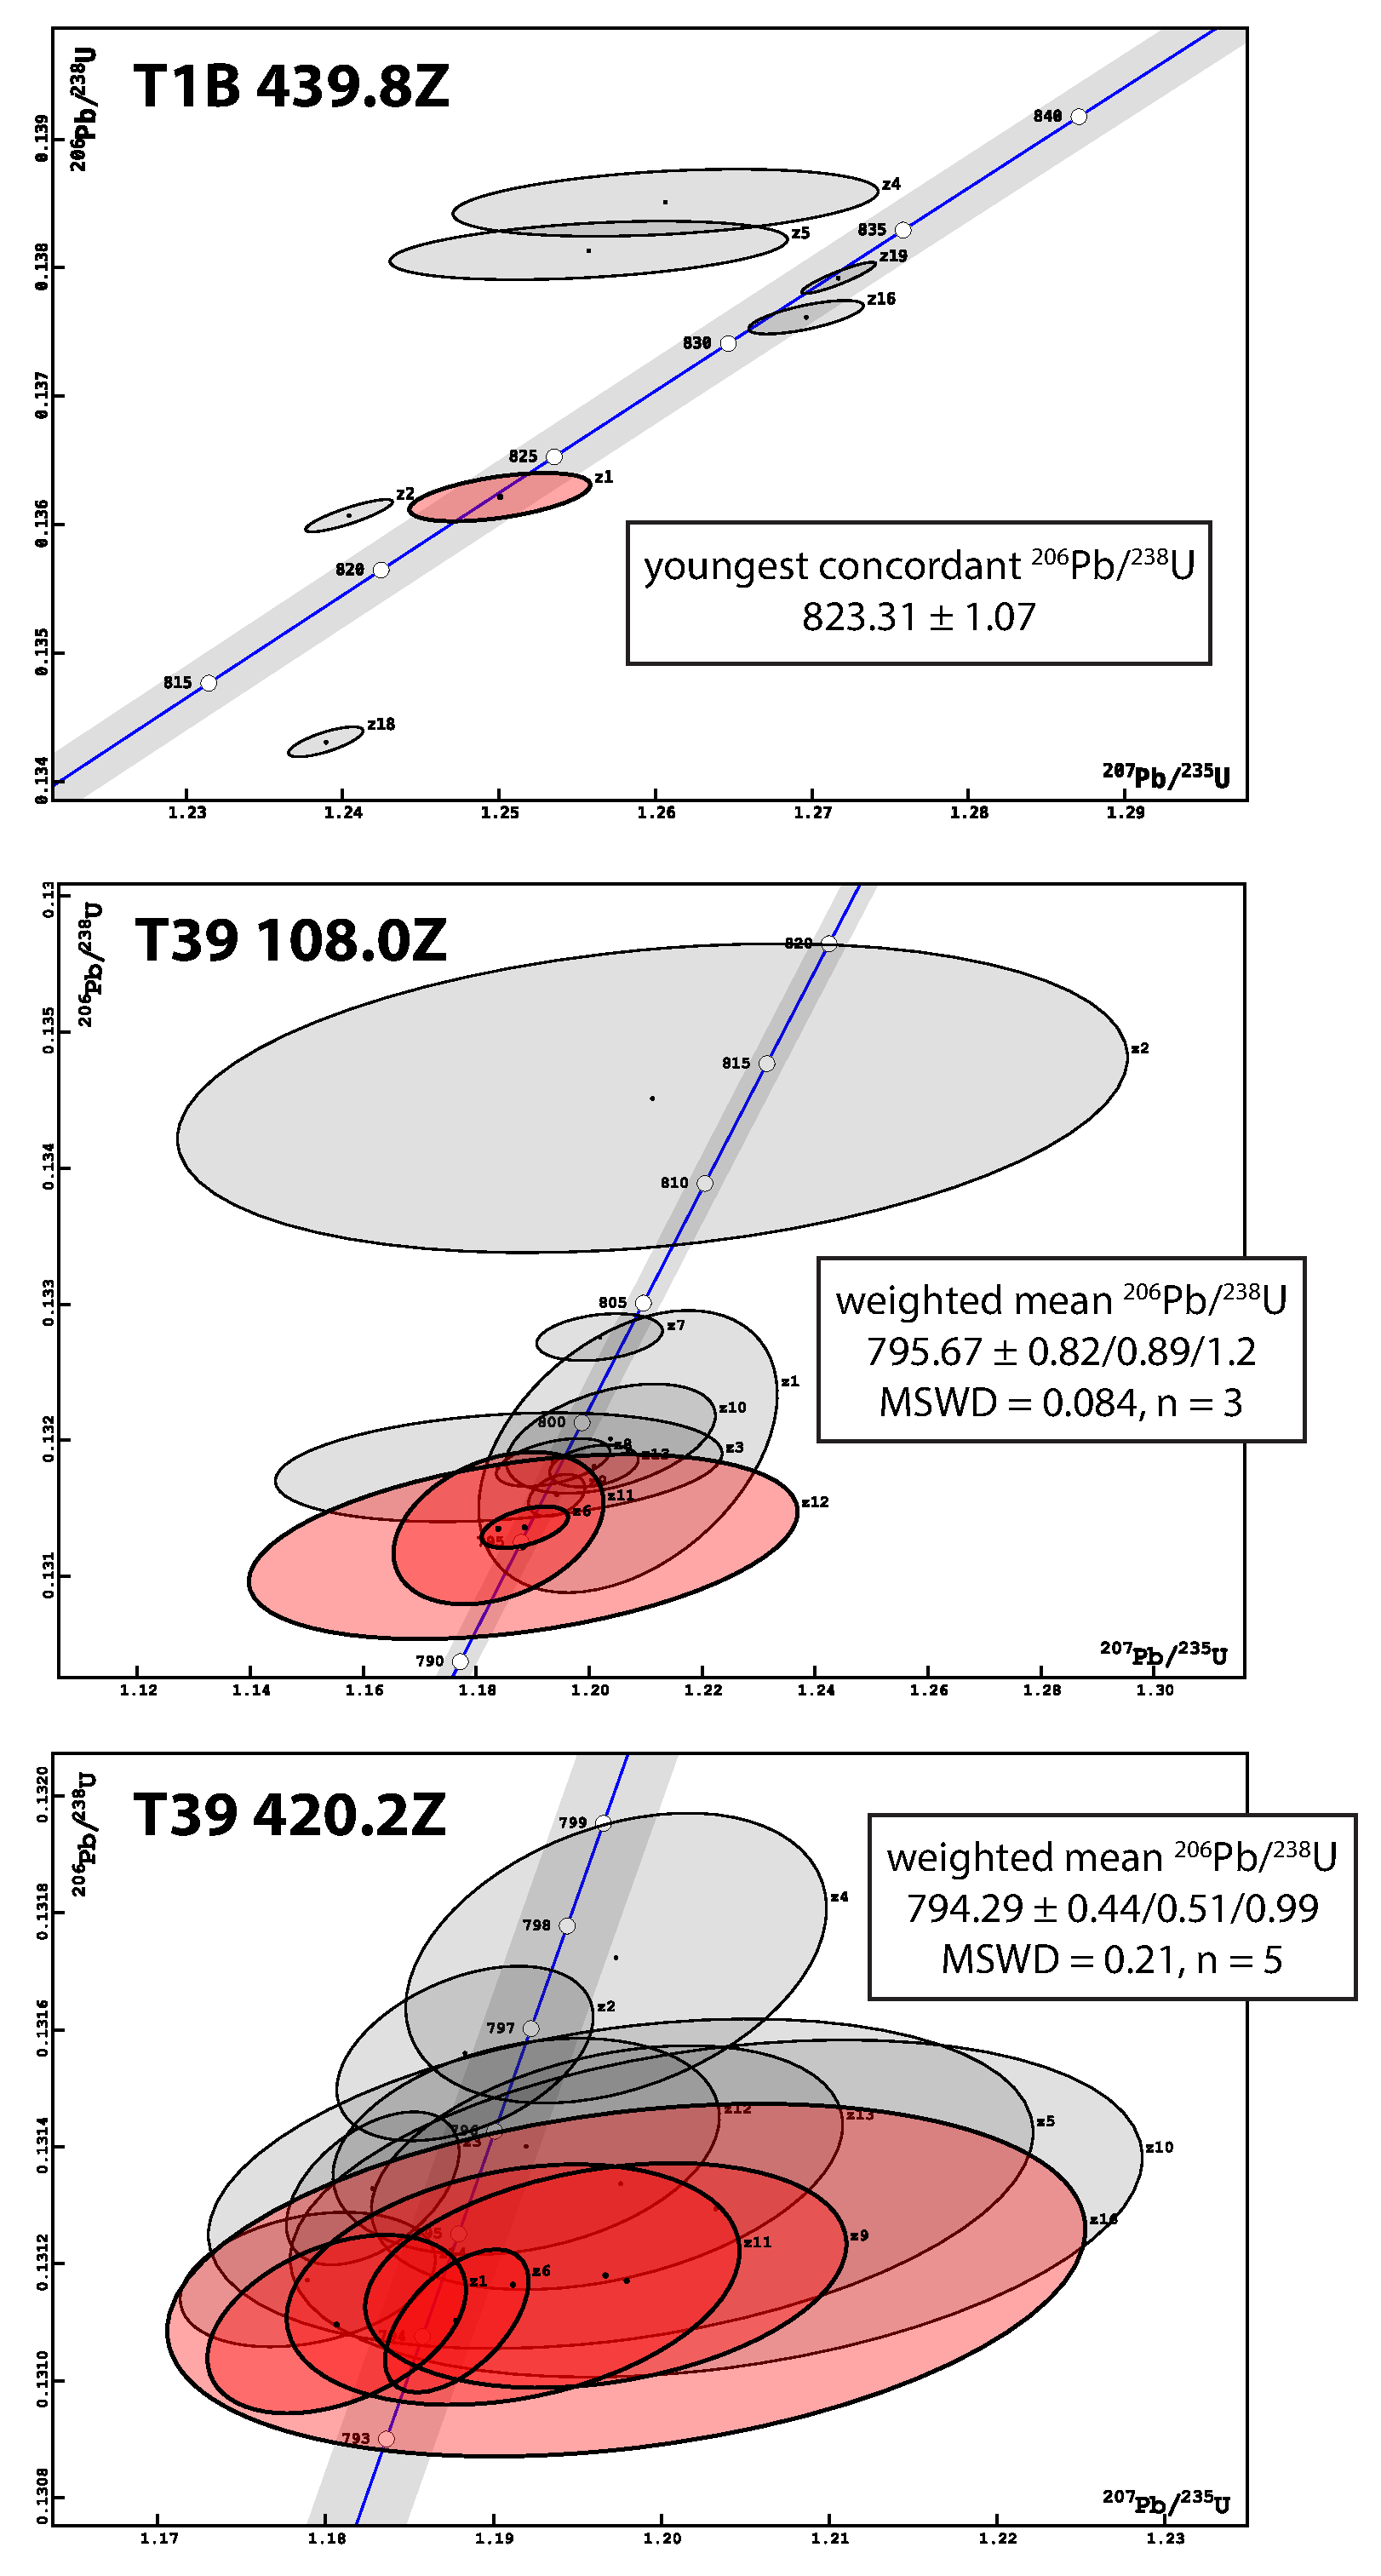
\includegraphics[width=0.5\textwidth]{figures/Tambien/concordia.pdf}
	\caption{Concordia diagrams for dates reported in this study. 2$\sigma$ uncertainties are reported in the format $\pm$X/Y/Z, where X is the internal (analytical) uncertainty in the absence of all external or systematic errors, Y is the uncertainty incorporating the U-Pb tracer calibration error, and Z is the uncertainty including X and Y, as well as the uranium decay constant uncertainty; MSWD = mean square of weighted deviates; n = number of zircon analyses included in the calculated date.}
	\label{fig:concordia}
\end{center}
\end{figure}

\begin{sidewaystable*}
\scriptsize
\vspace*{1 cm}
\caption{U-Pb data for analyzed zircon from T1B-439.8Z.}
\vspace{1 cm}
\setlength\tabcolsep{3.5pt}
\begin{tabular}{cccccccccccccccccccc}
& \multicolumn{8}{l}{Dates (Ma)} & \multicolumn{4}{l}{Composition} & \multicolumn{7}{l}{Isotopic Ratios} \\
\cline{2-20}\\
& $^a$ & & $^b$ & & $^{a,b}$ & & & $^c$ & $^d$ & $^e$ & $^f$ & $^{g}$ & $^h$ & $^{a,i}$ & & $^{b,i}$ & & $^{a,b,i}$ & \\	
& \underline{$^{206}$Pb} & $\pm$ & \underline{$^{207}$Pb} & $\pm$ & \underline{$^{207}$Pb} & $\pm$ & corr. & & \underline{Th} & Pb\** & Pb$_c$ & \underline{Pb\**} & \underline{$^{206}$Pb} & \underline{$^{206}$Pb} & $\pm$ & \underline{$^{207}$Pb} & $\pm$ & \underline{$^{207}$Pb} & $\pm$ \\		
fraction & $^{238}$U & (2$\sigma$) & $^{235}$U & (2$\sigma$) & $^{206}$Pb & (2$\sigma$) & coef. & \% disc. & U & (pg) & (pg) & Pb$_c$ & $^{204}$Pb & $^{238}$Pb & (2$\sigma\%$) & $^{235}$U & (2$\sigma\%$) & $^{206}$Pb & (2$\sigma\%$) \\
\hline \\
\rowcolor{Yellow}
z1 & 823.31 & 1.07 & 823.43 & 2.61 & 823.76 & 8.55 & 0.51 & 0.10 & 0.34 & 23.13 & 0.61 & 37.96 & 2348.88 & 0.14 & 0.14 & 1.25 & 0.46 & 0.07 & 0.41 \\
z2 & 822.49 & 0.71 & 819.07 & 1.26 & 809.80 & 3.20 & 0.85 & -1.53 & 0.35 & 68.32 & 0.62 & 110.86 & 6810.02 & 0.14 & 0.09 & 1.24 & 0.22 & 0.07 & 0.15 \\
z4 & 836.29 & 1.48 & 828.20 & 6.10 & 806.54 & 21.58 & 0.33 & -3.65 & 0.53 & 13.16 & 0.86 & 15.23 & 908.36 & 0.14 & 0.19 & 1.26 & 1.08 & 0.07 & 1.03 \\
z5 & 834.19 & 1.29 & 825.99 & 5.72 & 803.99 & 20.17 & 0.37 & -3.72 & 0.67 & 13.33 & 0.80 & 16.67 & 958.46 & 0.14 & 0.16 & 1.26 & 1.01 & 0.07 & 0.96 \\
z16 & 831.24 & 0.74 & 832.22 & 1.64 & 834.86 & 4.89 & 0.69 & 0.47 & 0.65 & 13.75 & 0.22 & 61.23 & 3610.31 & 0.14 & 0.10 & 1.27 & 0.29 & 0.07 & 0.23 \\
z17 & 855.05 & 0.73 & 855.83 & 1.17 & 857.86 & 2.59 & 0.92 & 0.36 & 0.73 & 32.33 & 0.18 & 181.54 & 10466.28 & 0.14 & 0.09 & 1.32 & 0.20 & 0.07 & 0.12 \\
z18 & 812.48 & 0.67 & 818.40 & 1.08 & 834.51 & 2.95 & 0.73 & 2.67 & 0.75 & 42.34 & 0.32 & 130.41 & 7480.36 & 0.13 & 0.09 & 1.24 & 0.19 & 0.07 & 0.14 \\
z19 & 832.98 & 0.69 & 833.16 & 1.06 & 833.64 & 2.36 & 0.90 & 0.12 & 0.57 & 47.38 & 0.18 & 266.55 & 15958.64 & 0.14 & 0.09 & 1.27 & 0.19 & 0.07 & 0.11 \\
\end{tabular}

\flushleft \emph{Notes:} \\
Colored rows indicate fractions included in the calculation of the reported sample age. \\
Isotopic dates calculated using $\lambda$238 = 1.55125$\times$10$^{-10}$ and $\lambda$235 = 9.8485$\times$10$^{-10}$ \citep{Jaffey1971a}. \\
 $^{a}$  Corrected for initial Th/U disequilibrium using radiogenic $^{208}$Pb and Th/U[magma] = 3.50000. \\
 $^{b}$ Corrected for initial Pa/U disequilibrium using initial fraction activity ratio [$^{231}$Pa]/[$^{235}$U] = 1.10000. \\
 $^{c}$ \% discordance = 100 - (100 $\times$ ($^{206}$Pb/$^{238}$U date) / ($^{207}$Pb/$^{206}$Pb date)) \\
 $^{d}$ Th contents calculated from radiogenic $^{208}$Pb and $^{230}$Th-corrected $^{206}$Pb/$^{238}$U date of the sample, assuming concordance between U-Pb Th-Pb systems. \\
 $^{e}$ Total mass of radiogenic Pb. \\
 $^{f}$ Total mass of common Pb. \\
 $^{g}$ Ratio of radiogenic Pb (including $^{208}$Pb) to common Pb. \\
 $^{h}$ Measured ratio corrected for fractionation and spike contribution only. \\
 $^{i}$ Measured ratios corrected for fractionation, tracer and blank.
\end{sidewaystable*}

\begin{sidewaystable*}
\scriptsize
\vspace*{1 cm}
\caption{U-Pb data for analyzed zircon from T39-108.0Z.}
\vspace{1 cm}
\setlength\tabcolsep{3.5pt}
\begin{tabular}{cccccccccccccccccccc}
& \multicolumn{8}{l}{Dates (Ma)} & \multicolumn{4}{l}{Composition} & \multicolumn{7}{l}{Isotopic Ratios} \\
\cline{2-20}\\
& $^a$ & & $^b$ & & $^{a,b}$ & & & $^c$ & $^d$ & $^e$ & $^f$ & $^{g}$ & $^h$ & $^{a,i}$ & & $^{b,i}$ & & $^{a,b,i}$ & \\	
& \underline{$^{206}$Pb} & $\pm$ & \underline{$^{207}$Pb} & $\pm$ & \underline{$^{207}$Pb} & $\pm$ & corr. & & \underline{Th} & Pb\** & Pb$_c$ & \underline{Pb\**} & \underline{$^{206}$Pb} & \underline{$^{206}$Pb} & $\pm$ & \underline{$^{207}$Pb} & $\pm$ & \underline{$^{207}$Pb} & $\pm$ \\		
fraction & $^{238}$U & (2$\sigma$) & $^{235}$U & (2$\sigma$) & $^{206}$Pb & (2$\sigma$) & coef. & \% disc. & U & (pg) & (pg) & Pb$_c$ & $^{204}$Pb & $^{238}$Pb & (2$\sigma\%$) & $^{235}$U & (2$\sigma\%$) & $^{206}$Pb & (2$\sigma\%$) \\
\hline \\
z1 & 798.88 & 5.90 & 803.74 & 12.16 & 817.26 & 41.88 & 0.41 & 2.29 & 0.57 & 1.59 & 0.25 & 6.29 & 395.48 & 0.13 & 0.79 & 1.21 & 2.19 & 0.07 & 2.00 \\
z2 & 813.64 & 6.45 & 805.73 & 38.62 & 783.94 & 142.22 & 0.26 & -3.75 & 0.56 & 0.54 & 0.30 & 1.78 & 125.78 & 0.13 & 0.84 & 1.21 & 6.94 & 0.07 & 6.77 \\
z3 & 798.22 & 2.28 & 793.16 & 18.38 & 778.96 & 68.88 & 0.25 & -2.43 & 0.51 & 4.01 & 1.13 & 3.54 & 233.74 & 0.13 & 0.30 & 1.18 & 3.34 & 0.07 & 3.28 \\
\rowcolor{Yellow}
z6 & 795.71 & 0.87 & 795.30 & 3.56 & 794.14 & 12.54 & 0.49 & -0.16 & 0.47 & 5.66 & 0.27 & 20.81 & 1297.81 & 0.13 & 0.12 & 1.19 & 0.65 & 0.07 & 0.60 \\
z7 & 803.66 & 0.98 & 801.43 & 5.14 & 795.22 & 18.90 & 0.27 & -1.02 & 0.43 & 4.03 & 0.31 & 12.82 & 813.30 & 0.13 & 0.13 & 1.20 & 0.93 & 0.07 & 0.90 \\
z8 & 798.42 & 1.01 & 797.63 & 4.66 & 795.41 & 16.56 & 0.46 & -0.34 & 0.58 & 5.09 & 0.31 & 16.30 & 993.36 & 0.13 & 0.13 & 1.19 & 0.84 & 0.07 & 0.79 \\
z9 & 797.04 & 0.88 & 797.93 & 2.31 & 800.40 & 8.21 & 0.36 & 0.46 & 0.73 & 12.47 & 0.33 & 38.31 & 2223.30 & 0.13 & 0.12 & 1.19 & 0.42 & 0.07 & 0.39 \\
z10 & 799.42 & 2.28 & 802.34 & 8.53 & 810.47 & 30.06 & 0.42 & 1.40 & 0.50 & 2.01 & 0.20 & 10.01 & 628.68 & 0.13 & 0.30 & 1.20 & 1.54 & 0.07 & 1.44 \\
\rowcolor{Yellow}
z11 & 795.67 & 3.19 & 793.15 & 8.65 & 786.05 & 31.21 & 0.33 & -1.18 & 0.44 & 2.11 & 0.27 & 7.93 & 509.16 & 0.13 & 0.43 & 1.18 & 1.57 & 0.07 & 1.49 \\
\rowcolor{Yellow}
z12 & 794.90 & 3.87 & 795.18 & 22.55 & 795.97 & 82.26 & 0.38 & 0.18 & 0.42 & 1.37 & 0.39 & 3.54 & 238.72 & 0.13 & 0.52 & 1.19 & 4.09 & 0.07 & 3.92 \\
z13 & 798.28 & 0.88 & 800.97 & 3.63 & 808.48 & 13.15 & 0.31 & 1.30 & 0.43 & 5.40 & 0.28 & 19.34 & 1218.11 & 0.13 & 0.12 & 1.20 & 0.65 & 0.07 & 0.63 \\
\end{tabular}

\flushleft \emph{Notes:} \\
Colored rows indicate fractions included in the calculation of the reported sample age. \\
Isotopic dates calculated using $\lambda$238 = 1.55125$\times$10$^{-10}$ and $\lambda$235 = 9.8485$\times$10$^{-10}$ \citep{Jaffey1971a}. \\
 $^{a}$  Corrected for initial Th/U disequilibrium using radiogenic $^{208}$Pb and Th/U[magma] = 3.50000. \\
 $^{b}$ Corrected for initial Pa/U disequilibrium using initial fraction activity ratio [$^{231}$Pa]/[$^{235}$U] = 1.10000. \\
 $^{c}$ \% discordance = 100 - (100 $\times$ ($^{206}$Pb/$^{238}$U date) / ($^{207}$Pb/$^{206}$Pb date)) \\
 $^{d}$ Th contents calculated from radiogenic $^{208}$Pb and $^{230}$Th-corrected $^{206}$Pb/$^{238}$U date of the sample, assuming concordance between U-Pb Th-Pb systems. \\
 $^{e}$ Total mass of radiogenic Pb. \\
 $^{f}$ Total mass of common Pb. \\
 $^{g}$ Ratio of radiogenic Pb (including $^{208}$Pb) to common Pb. \\
 $^{h}$ Measured ratio corrected for fractionation and spike contribution only. \\
 $^{i}$ Measured ratios corrected for fractionation, tracer and blank.
\end{sidewaystable*}

\begin{sidewaystable*}
\scriptsize
\vspace*{1 cm}
\caption{U-Pb data for analyzed zircon from T39-420.2Z.}
\vspace{1 cm}
\setlength\tabcolsep{3.5pt}
\begin{tabular}{cccccccccccccccccccc}
& \multicolumn{8}{l}{Dates (Ma)} & \multicolumn{4}{l}{Composition} & \multicolumn{7}{l}{Isotopic Ratios} \\
\cline{2-20}\\
& $^a$ & & $^b$ & & $^{a,b}$ & & & $^c$ & $^d$ & $^e$ & $^f$ & $^{g}$ & $^h$ & $^{a,i}$ & & $^{b,i}$ & & $^{a,b,i}$ & \\	
& \underline{$^{206}$Pb} & $\pm$ & \underline{$^{207}$Pb} & $\pm$ & \underline{$^{207}$Pb} & $\pm$ & corr. & & \underline{Th} & Pb\** & Pb$_c$ & \underline{Pb\**} & \underline{$^{206}$Pb} & \underline{$^{206}$Pb} & $\pm$ & \underline{$^{207}$Pb} & $\pm$ & \underline{$^{207}$Pb} & $\pm$ \\		
fraction & $^{238}$U & (2$\sigma$) & $^{235}$U & (2$\sigma$) & $^{206}$Pb & (2$\sigma$) & coef. & \% disc. & U & (pg) & (pg) & Pb$_c$ & $^{204}$Pb & $^{238}$Pb & (2$\sigma\%$) & $^{235}$U & (2$\sigma\%$) & $^{206}$Pb & (2$\sigma\%$) \\
\hline \\
\rowcolor{Yellow}
z1 & 794.12 & 0.87 & 791.62 & 3.59 & 784.58 & 12.98 & 0.38 & -1.18 & 0.69 & 11.98 & 0.49 & 24.28 & 1391.39 & 0.13 & 0.12 & 1.18 & 0.65 & 0.07 & 0.62 \\
z2 & 796.76 & 0.85 & 795.17 & 3.55 & 790.74 & 12.69 & 0.42 & -0.73 & 0.87 & 15.22 & 0.59 & 25.79 & 1415.45 & 0.13 & 0.11 & 1.19 & 0.64 & 0.07 & 0.60 \\
z3 & 795.44 & 0.75 & 792.62 & 2.40 & 784.69 & 8.35 & 0.48 & -1.33 & 0.76 & 23.62 & 0.59 & 40.01 & 2239.52 & 0.13 & 0.10 & 1.18 & 0.44 & 0.07 & 0.40 \\
z4 & 797.69 & 1.41 & 799.35 & 5.80 & 803.97 & 20.92 & 0.34 & 0.82 & 0.73 & 13.69 & 0.91 & 15.02 & 857.80 & 0.13 & 0.19 & 1.20 & 1.05 & 0.07 & 1.00 \\
z5 & 795.49 & 1.61 & 799.47 & 11.36 & 810.60 & 41.75 & 0.31 & 1.90 & 0.64 & 12.24 & 1.71 & 7.15 & 427.13 & 0.13 & 0.21 & 1.20 & 2.05 & 0.07 & 2.00 \\
\rowcolor{Yellow}
z6 & 794.15 & 0.70 & 794.95 & 1.99 & 797.18 & 6.68 & 0.55 & 0.42 & 0.77 & 43.52 & 0.87 & 50.28 & 2801.05 & 0.13 & 0.09 & 1.19 & 0.36 & 0.07 & 0.32 \\
\rowcolor{Yellow}
z9 & 794.59 & 1.09 & 799.06 & 6.63 & 811.54 & 24.38 & 0.28 & 2.12 & 1.20 & 8.79 & 0.62 & 14.19 & 731.99 & 0.13 & 0.15 & 1.20 & 1.20 & 0.07 & 1.17 \\
z10 & 795.25 & 1.64 & 802.10 & 11.70 & 821.19 & 42.92 & 0.30 & 3.19 & 1.06 & 10.65 & 1.38 & 7.70 & 416.84 & 0.13 & 0.22 & 1.20 & 2.11 & 0.07 & 2.06 \\
\rowcolor{Yellow}
z11 & 794.51 & 1.17 & 796.51 & 6.26 & 802.10 & 23.04 & 0.28 & 0.98 & 0.69 & 5.42 & 0.40 & 13.43 & 776.60 & 0.13 & 0.16 & 1.19 & 1.13 & 0.07 & 1.10 \\
z12 & 795.85 & 1.05 & 796.87 & 5.34 & 799.70 & 19.65 & 0.27 & 0.51 & 1.16 & 10.71 & 0.61 & 17.46 & 903.55 & 0.13 & 0.14 & 1.19 & 0.97 & 0.07 & 0.94 \\
z13 & 795.65 & 1.19 & 799.10 & 6.49 & 808.72 & 23.61 & 0.35 & 1.65 & 0.66 & 5.25 & 0.40 & 13.04 & 760.42 & 0.13 & 0.16 & 1.20 & 1.17 & 0.07 & 1.13 \\
z14 & 794.55 & 0.66 & 790.82 & 3.54 & 780.29 & 13.14 & 0.29 & -1.80 & 1.30 & 10.90 & 0.40 & 27.31 & 1363.19 & 0.13 & 0.09 & 1.18 & 0.64 & 0.07 & 0.62 \\
\rowcolor{Yellow}
z16 & 794.55 & 1.72 & 799.63 & 12.64 & 813.80 & 46.60 & 0.29 & 2.40 & 0.66 & 7.30 & 1.14 & 6.40 & 382.41 & 0.13 & 0.23 & 1.20 & 2.28 & 0.07 & 2.23 \\
\end{tabular}

\flushleft \emph{Notes:} \\
Colored rows indicate fractions included in the calculation of the reported sample age. \\
Isotopic dates calculated using $\lambda$238 = 1.55125$\times$10$^{-10}$ and $\lambda$235 = 9.8485$\times$10$^{-10}$ \citep{Jaffey1971a}. \\
 $^{a}$  Corrected for initial Th/U disequilibrium using radiogenic $^{208}$Pb and Th/U[magma] = 3.50000. \\
 $^{b}$ Corrected for initial Pa/U disequilibrium using initial fraction activity ratio [$^{231}$Pa]/[$^{235}$U] = 1.10000. \\
 $^{c}$ \% discordance = 100 - (100 $\times$ ($^{206}$Pb/$^{238}$U date) / ($^{207}$Pb/$^{206}$Pb date)) \\
 $^{d}$ Th contents calculated from radiogenic $^{208}$Pb and $^{230}$Th-corrected $^{206}$Pb/$^{238}$U date of the sample, assuming concordance between U-Pb Th-Pb systems. \\
 $^{e}$ Total mass of radiogenic Pb. \\
 $^{f}$ Total mass of common Pb. \\
 $^{g}$ Ratio of radiogenic Pb (including $^{208}$Pb) to common Pb. \\
 $^{h}$ Measured ratio corrected for fractionation and spike contribution only. \\
 $^{i}$ Measured ratios corrected for fractionation, tracer and blank.
\end{sidewaystable*}

\begin{figure}[h!]
\begin{center}
	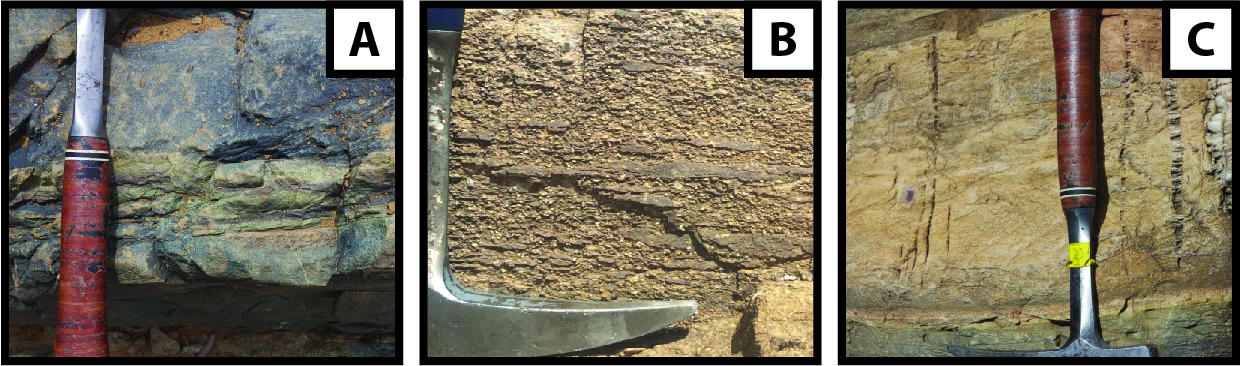
\includegraphics[width=\textwidth]{figures/Tambien/geochronology-photos.jpg}
	\caption{\textbf{(A)} Photograph of the lava flow T1b-439.8Z. \textbf{(B)} Photograph of the ignimbrite T39-108.0Z, with feldspar phenocrysts and fiammed lithic clasts. \textbf{(C)} Photograph of the 30~cm rhyolitic tuff T39-420.2Z, with normally graded lapilli at the base. Hammer points up section in all panels.}
	\label{fig:geochronology-photos}
\end{center}
\end{figure}

\clearpage

\section{Diagenetic Considerations}

\subsection{Isotope Conglomerate Test}

\begin{figure}[h!]
\begin{center}
	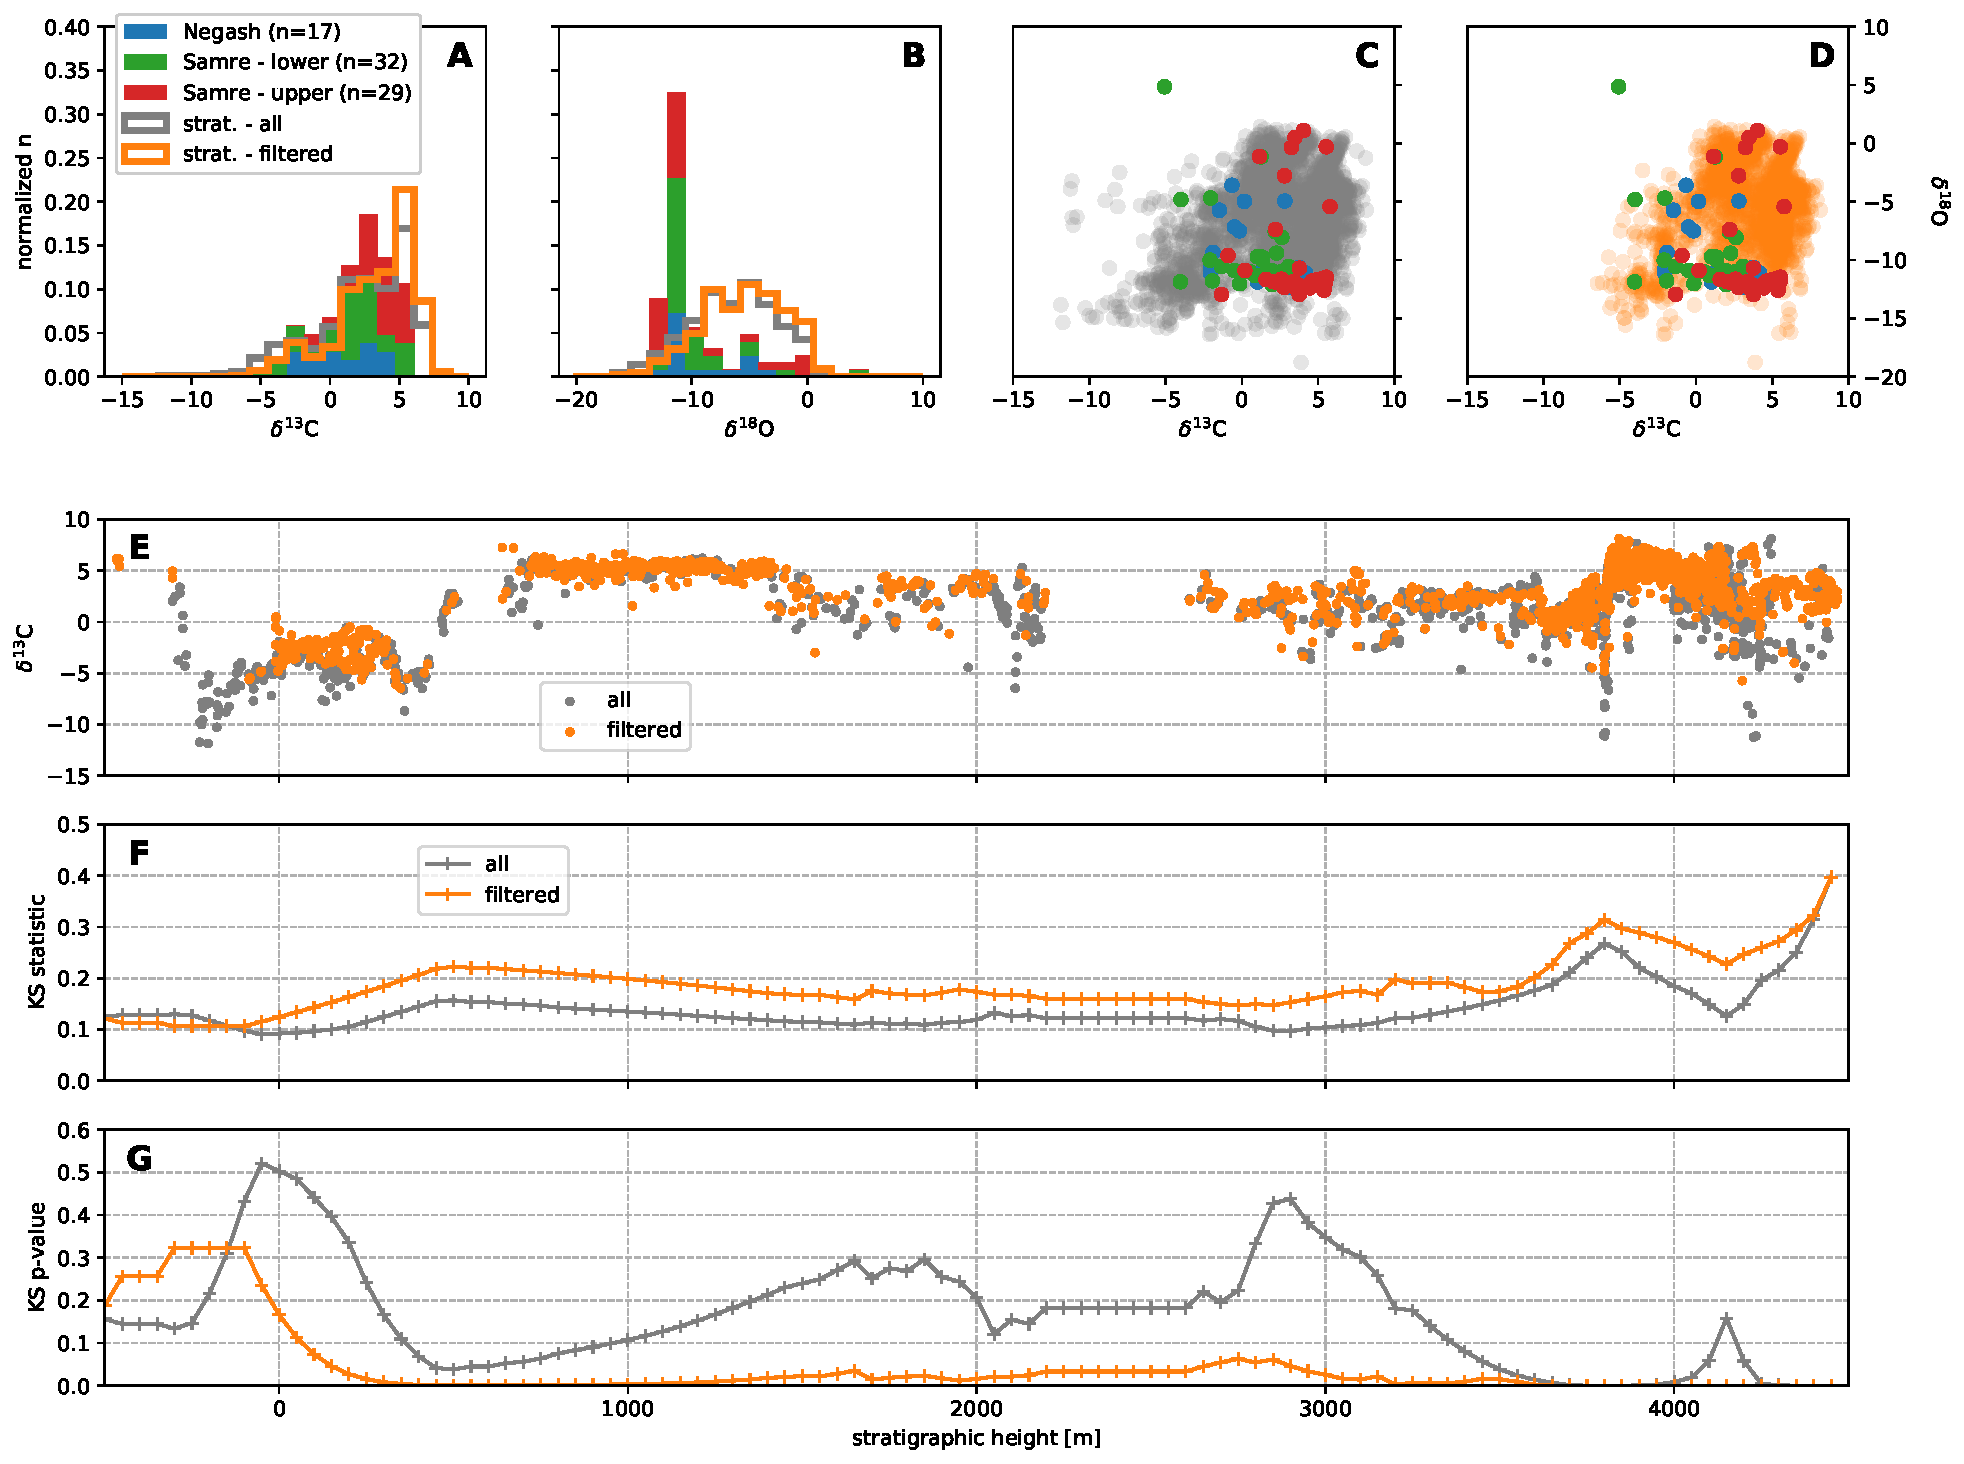
\includegraphics[width=\textwidth]{figures/Tambien/clast-analysis-pval.pdf}
	\caption{\textbf{(A)} and \textbf{(B)} Histograms of \dC and \dO values of carbonate clasts within the diamictite of the Negash Formation of both the Negash Syncline and Samre Fold-Thrust Belt, compared to all \textit{in situ} Tambien Group carbonate samples. Both filtered and unfiltered (all) versions of the \textit{in situ} carbonate data are shown (see main text for a discussion of the filtering method). \textbf{(C)} and \textbf{(D)} Cross plots of \dC vs \dO for the clasts and \textit{in situ} carbonate samples. \textbf{(E)} Filtered and unfiltered versions of the \textit{in situ} carbonate \dC data against cumulative stratigraphic height. \textbf{(F)} Degree of correlation (as quantified by the Kolgomorov-Smirnov statistic) between the \textit{in situ} carbonate \dC data with the carbonate clasts within the diamictite as samples below a given cumulative stratigraphic height (x-axis) are removed (i.e. the x-axis represents the depth of erosion). Low values suggest that the two datasets are drawn from the same distribution. See accompanying text for further details. \textbf{(G)} Kolgomorov-Smirnov statistic p-value. High values suggest that the two datasets are drawn from the same distribution.}
	\label{fig:clast-analysis-pval}
\end{center}
\end{figure}

We compare \dC and \dO values of the carbonate clasts from within diamictite of the Negash Formation of the Negash Syncline and Samre Fold-Thrust Belt. In general, the distribution of clast \dC values is similar to that of the \textit{in situ} Tambien Group carbonates (Fig. \ref{fig:clast-analysis-pval}A). However, the filtering technique proposes that the stratigraphic distance of a sample to the closest siliciclastic unit is a reasonable predictor for \dC alteration in \textit{in situ} Tambien Group carbonates. If such a scenario applied equally to the diamictite clasts, we might expect the \dC of the clasts to be pulled to more negative values relative to the \textit{in situ} carbonates since most of the samples in the \textit{in situ} stratigraphy were extracted from carbonate horizons thicker than the diamictite clasts, but such a distribution is not observed.

There are several potential explanations for this apparent inconsistency. First, as discussed in the main text, samples that fall below the threshold \dsil may or may not have had their carbon isotopic composition altered. And so, even though the majority of sampled diamictite clasts have a radius \textless0.2~m, the \dC of a significant proportion of these samples need not have been affected by secondary alteration. Second, it is possible that carbon is better buffered in the diamictite relative to the rest of the Tambien Group. Unless 100\% of the diamictite's matrix was produced via scouring and redeposition of pre-Snowball Earth siliciclastics with associated organic matter, the matrix likely contains less low \dC organic carbon relative to the siliciclastic units of the underlying Tambien Group, given that organic productivity was suppressed during the Snowball Earth \citep{Hoffman2017a}. The presence of extra-basinal clasts within the diamictite (see main text) suggests that at least some of the protolith was sourced from distal bedrock, and thus the organic component of the diamictite's matrix was likely diluted relative to undisturbed Tambien Group siliciclastics. Third, given that glacial erosion generates a bimodal sediment size distribution (fine grains from scouring and larger clasts from plucking) from the same rock, the sampled carbonate clasts in the diamictite are likely accompanied by fine carbonate sand from the same rock. This relatively carbonate-rich diamictite matrix would help to buffer the carbon isotopic composition of diamictite clasts against changes in \dC in a way that siliciclastic units within the \textit{in situ} Tambien Group stratigraphy would not be able to. Finally, it is possible that our sampling of clasts from the diamictite is not representative of the bulk population. The total number of diamictite clasts sampled (n = 78) is substantially smaller than the total number of samples from \textit{in situ} Tambien Group carbonates (n = 3139). Furthermore, diamictite clasts were only sampled from three discrete stratigraphic horizons, which may have been more carbonate buffered relative to the rest of the diamictite.

\dO values of the diamictite clasts are distinctly different from the spread in values observed in the \textit{in situ} stratigraphy, and cluster at $\sim$-12\permil (Fig. \ref{fig:clast-analysis-pval}B). This difference suggests that, unlike the carbon isotopic composition, the oxygen isotope composition of the carbonate clasts was significantly more overprinted following deposition of the diamictite than that of the \textit{in situ} carbonates. This difference in post-depositional alteration likely arises from the fact that the carbonate clasts in the diamictite are embedded within a predominantly siliciclastic matrix and are therefore less carbonate buffered against altering fluids, whereas most of the samples in the \textit{in situ} stratigraphy were extracted from carbonate horizons thicker than the diamictite clasts and are therefore more likely to be carbonate buffered. Since carbon is more rock-buffered against altering fluids than oxygen, the \dC of the clasts are more likely to preserve primary values.

Glacial erosion during the Sturtian Glaciation likely preferentially eroded the upper Tambien Group in most places instead of eroding all the way to the base of the Tambien Group. To assess how deep the bulk of glaciers eroded into Tambien Group stratigraphy, we divided the Tambien Group chemostratigraphic composite data collected from the \textit{in situ} stratigraphy (Fig. \ref{fig:clast-analysis-pval}E) into several equal length (50~m) stratigraphic windows, and randomly selected the same number of samples from each of these windows. This Monte Carlo approach is necessary to avoid bias toward relatively heavily sampled intervals of the stratigraphy. We then quantified the similarity in distributions between the \dC of the Monte Carlo sampled \textit{in situ} stratigraphy with that of the diamictite clasts using the two sample Kolmogorov-Smirnov (KS) statistic, which tests whether two sets of samples are consistent with being drawn from the same distribution. Low KS statistics and high p-values suggest that the two samples are drawn from the same distribution. We then simulate shallower erosion by iteratively excluding the lowest of these stratigraphic windows and recalculating the KS statistic, moving up the stratigraphy (Fig. \ref{fig:clast-analysis-pval}F and G). In general, we find that the two distributions are closest when the `erosion height' is close to the bottom of the Tambien Group ($\sim$0~m in Fig. \ref{fig:clast-analysis-pval}F and G) and near the middle of the Tambien Group ($\sim$2900~m). We also observe a distinct trough/peak near the top of the Tambien Group ($\sim$4200~m), although the KS statistic/p-value is not as low/high as at the bottom or near the middle of the Tambien Group. Furthermore, the filtered version of the \textit{in situ} carbonate \dC data (see main text) matches the clast data more poorly than all of the \textit{in situ} carbonate \dC data, likely as a result of similar post-depositional alteration mechanisms operating throughout the entirety of the Tambien Group. Ultimately, this analysis illustrates the fact that a relatively large proportion of the diamictite clasts have relatively low \dC (\textless0\permil), and thus the clast \dC distribution matches the \textit{in situ} carbonate \dC distribution when the `erosion height' is such that it includes a high proportion of samples within the Bitter Springs stage, the Didikama-Matheos excursion, and/or carbonate samples that have likely experienced secondary alteration pulling them to lower \dC values. Observations of the facies of clasts within the diamictite suggest that they were sourced predominantly from the Matheos and/or Mariam Bohkahko formations (see main text), and thus an `erosion height' of $\sim$2900~m or $\sim$4200~m would be consistent with these facies. The KS statistic/p-value at these `erosion heights' is low/high enough such that we cannot reject the null hypothesis that the diamictite clasts and the \textit{in situ} carbonate samples from above these heights come from the same distribution. However, we note that erosion into the Mariam Bohkahko/Matheos formations is not observed locally where the diamictite is deposited. This observation requires that the clasts derive from carbonates time-equivalent to these formations deposited elsewhere in the basin, or from carbonates deposited in another basin within an Arabian-Nubian terrane.

\clearpage

\subsection{Sample Proximity to Siliciclastic Units}

\begin{figure}[h!]
\begin{center}
	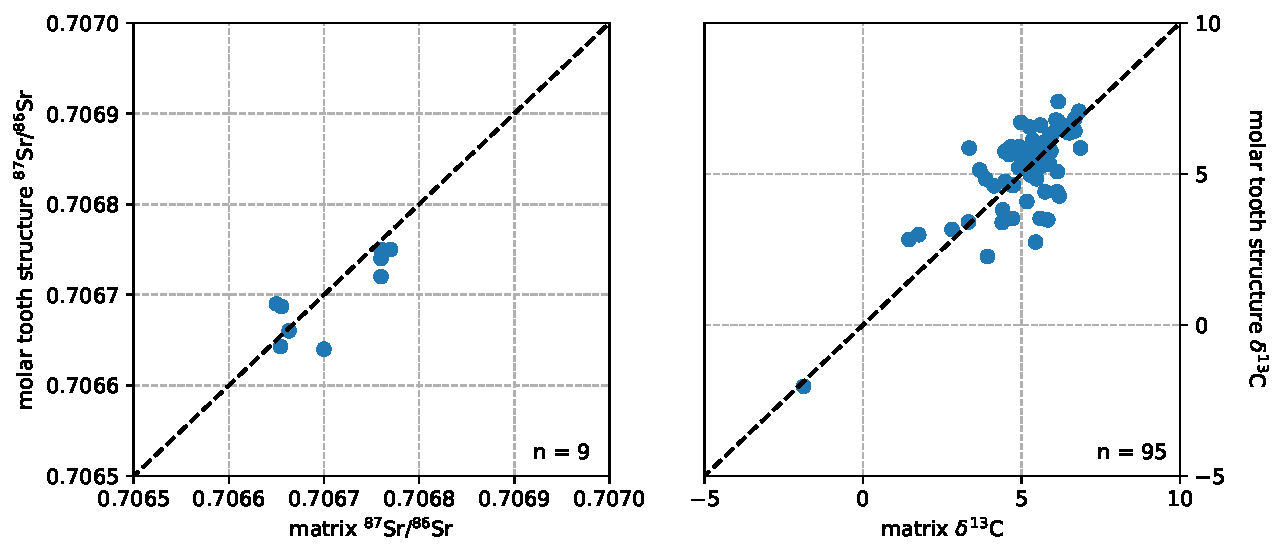
\includegraphics[width=0.7\textwidth]{figures/Tambien/MTS-MTX-comparison.pdf}
	\caption{Cross plots of carbonate matrix vs. adjacent molar tooth structure calcite \SrSr and \dC from Tambien Group samples that meet the filtering thresholds for alteration (see main text). Dashed black lines are the 1:1 lines - samples that fall on these lines have identical isotopic composition between the matrix and molar tooth structure carbonate. The isotopic composition of the matrix is similar to that of adjacent molar tooth structures, and no systematic offsets can be identified.}
	\label{fig:MTS-MTX-comparison}
\end{center}
\end{figure}

\begin{figure}[h!]
\begin{center}
	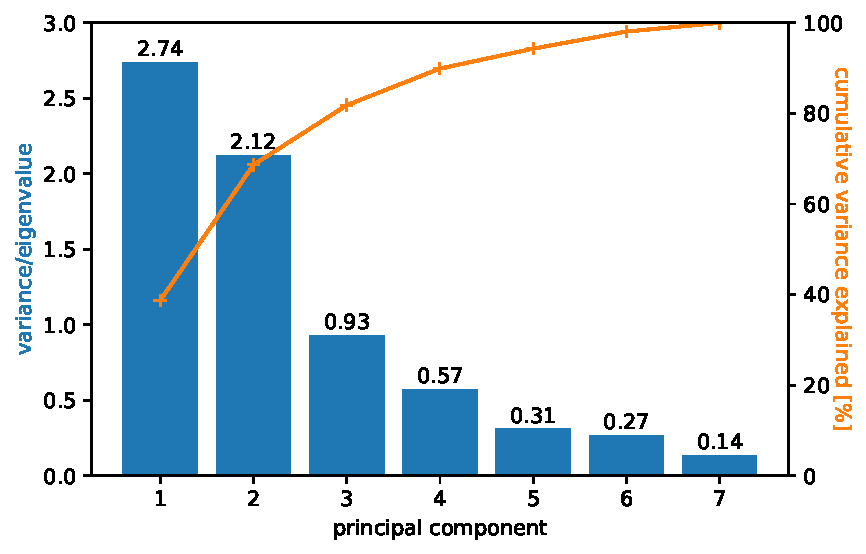
\includegraphics[width=0.5\textwidth]{figures/Tambien/siliciclastic-filtering-components.pdf}
	\caption{Eigenvalues and cumulative variance explained for the 7 principal components in the principal components analysis (also known as a scree plot). Notably, the magnitude of the eigenvalues (and the percent variance explained) drops off sharply after the second principal component, indicating that the first two principal components capture the most significant sources of variance in our dataset.}
	\label{fig:siliciclastic-filtering-components}
\end{center}
\end{figure}

\begin{figure}[h!]
\begin{center}
	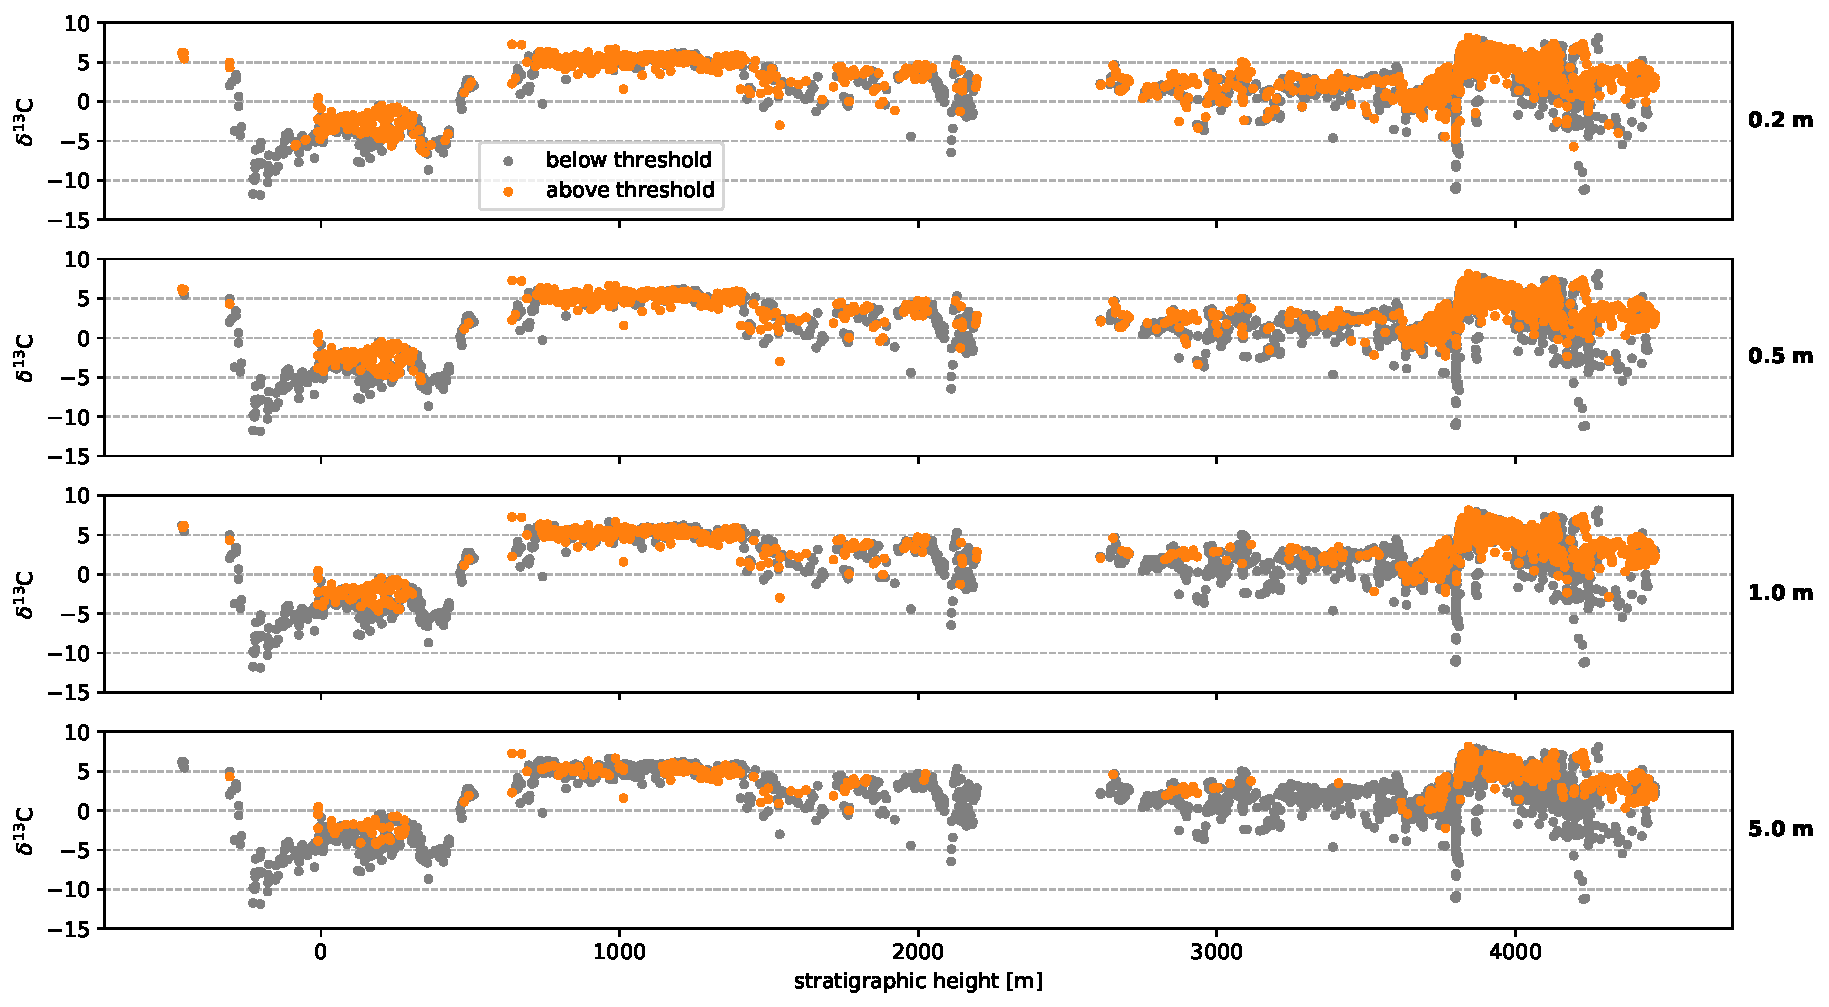
\includegraphics[width=\textwidth]{figures/Tambien/siliciclastic-filtering-comparison.pdf}
	\caption{Resulting composite chemostratigraphy of the Tambien Group as samples below a given \dsil (shown on the right) are filtered out. Note that data that resolve the Didikama-Matheos excursion as well as the descent into and recovery out of the Bitter Springs stage are mostly removed under the \dsil = 0.2~m threshold, and completely removed by \dsil = 0.5~m.}
	\label{fig:siliciclastic-filtering-comparison}
\end{center}
\end{figure}

\begin{figure}[h!]
\begin{center}
	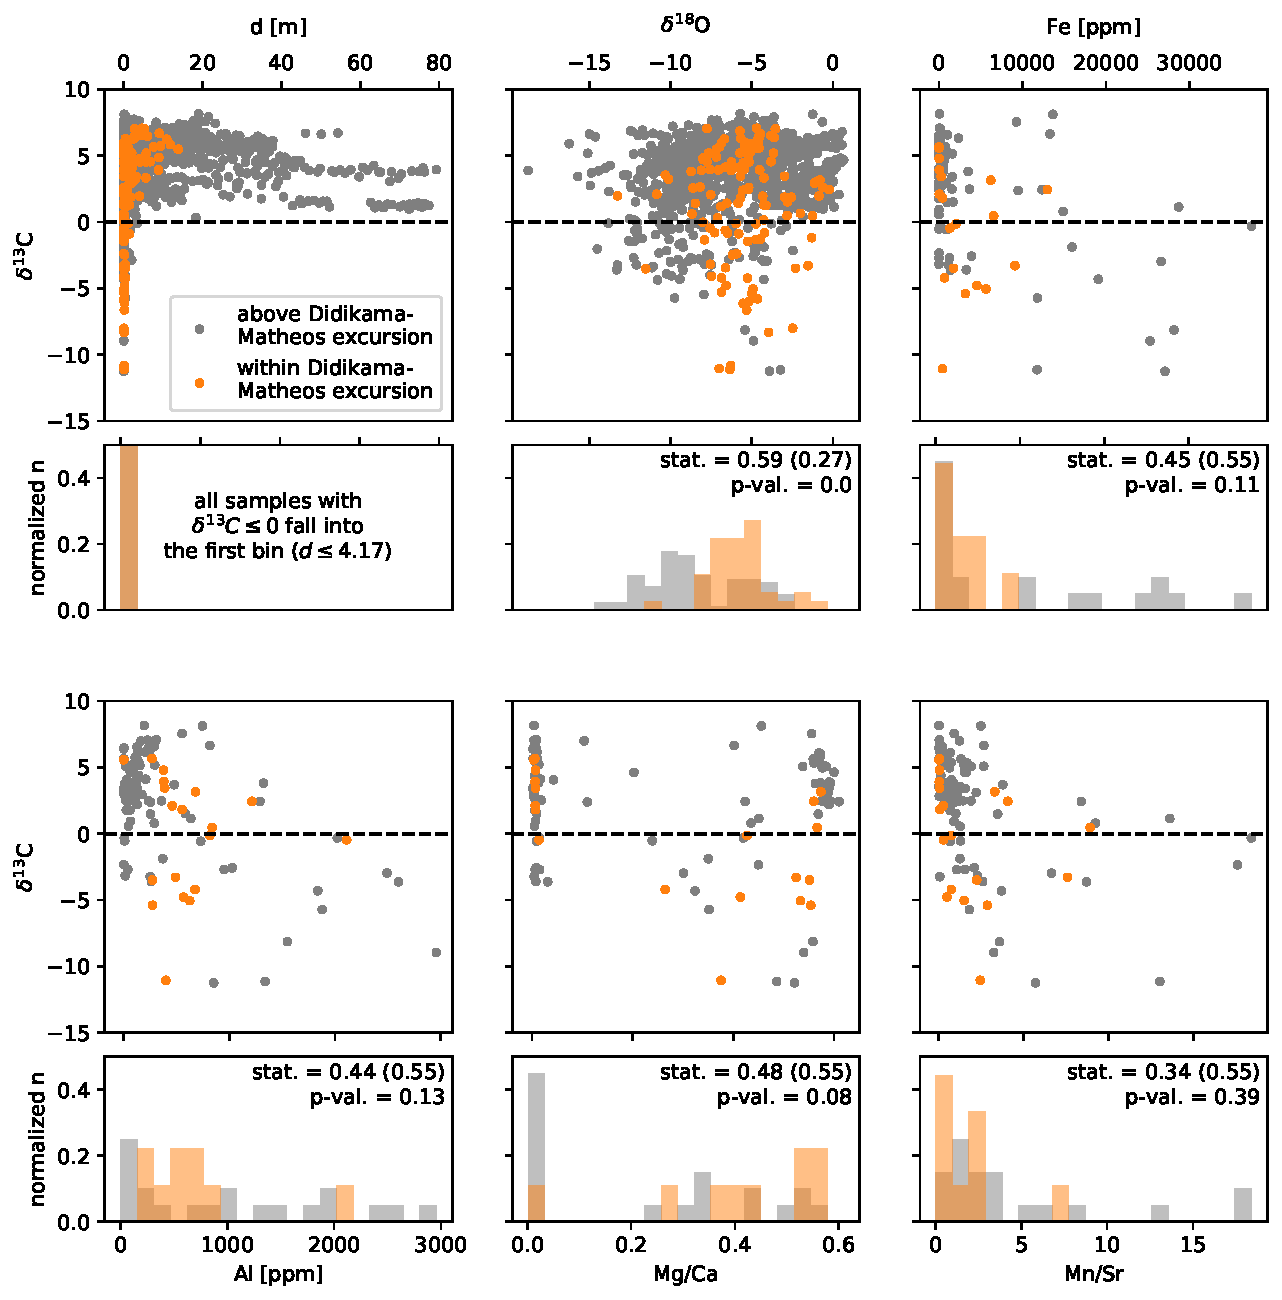
\includegraphics[width=\textwidth]{figures/Tambien/siliciclastic-filtering-DidiMath-excursion.pdf}
	\caption{Comparison of individual samples above the Didikama-Matheos excursion vs. samples within/adjacent to the Didikama-Matheos excursion. The normalized histograms under each scatter plot compare the distribution of samples with \dC$\leq$0\permil only. The `stat.' and `p-val.' refer to the Kolmogorov-Smirnov statistic and p-value respectively, with the value within the parentheses showing the critical Kolmogorov-Smirnov statistic for rejecting the null hypothesis (see text below).}
	\label{fig:siliciclastic-filtering-DidiMath-excursion}
\end{center}
\end{figure}

\clearpage

As per conventions in statistics, the following discussion will use the term `unit' to refer to an individual carbonate rock, and the term `sample' to refer to a collection of `units' from a population. Figure \ref{fig:siliciclastic-filtering-DidiMath-excursion} compares geochemical data of units above the Didikama-Matheos excursion to units within/adjacent to the Didikama-Matheos excursion. Units within the Didikama-Matheos excursion that record \dC$\leq$0\permil appear to exhibit lower Fe, Al, and Mn/Sr than units that record \dC$\leq$0\permil above the Didikama-Matheos excursion. This difference in distributions suggests that low \dC Didikama-Matheos excursion units have been less altered by the unbuffered fluids (see main text) than low \dC post-Didikama-Matheos excursion units, and thus provides support for the primary nature of the anomaly. To quantify this qualitative interpretation of the data, we compare the distributions of units with low \dC above the Didikama-Matheos excursion to units with low \dC within the Didikama-Matheos excursion by computing the two-sample Kolmogorov-Smirnov (KS) statistic. We also compute the critical KS statistic for rejecting the null hypothesis, which is given by $1.36\sqrt{\frac{N_{1}+N_{2}}{N_{1}N_{2}}}$, where $N_{1}$ and $N_{2}$ are the number of items in the two samples. If the computed KS statistic is above the critical KS statistic, or the p-value is below 0.05, we can reject the null hypothesis at the 95\% confidence level that the two samples come from the same distribution. We find that the KS test yields ambiguous results for the Fe, Al, and Mn/Sr (Fig. \ref{fig:siliciclastic-filtering-DidiMath-excursion}). For all three variables, the KS statistic is below the critical value, and the p-value is above 0.05. These results indicate that we cannot declare at the 95\% confidence level that the two samples come from different distributions - instead, the test indicates that the samples may or may not come from the same distribution. However, the primary reason for this ambiguity is the small number of units used in the test. There are only 20 units with \dC$\leq$0\permil and element concentration data above the Didikama-Matheos excursion, and only 9 units with \dC$\leq$0\permil and element concentration within the Didikama-Matheos excursion, which results in a high critical KS statistic and thus a more `difficult' test to achieve an unambiguous result in. Therefore, more element concentration data is required in order for the KS test to quantitatively reject the hypothesis at the 95\% confidence level that units within the Didikama-Matheos excursion that record \dC$\leq$0\permil exhibit lower Fe, Al, and Mn/Sr than units that record \dC$\leq$0\permil above the Didikama-Matheos excursion.

\clearpage

\subsection{Sr Isotopes}

\begin{figure}[h!]
\begin{center}
	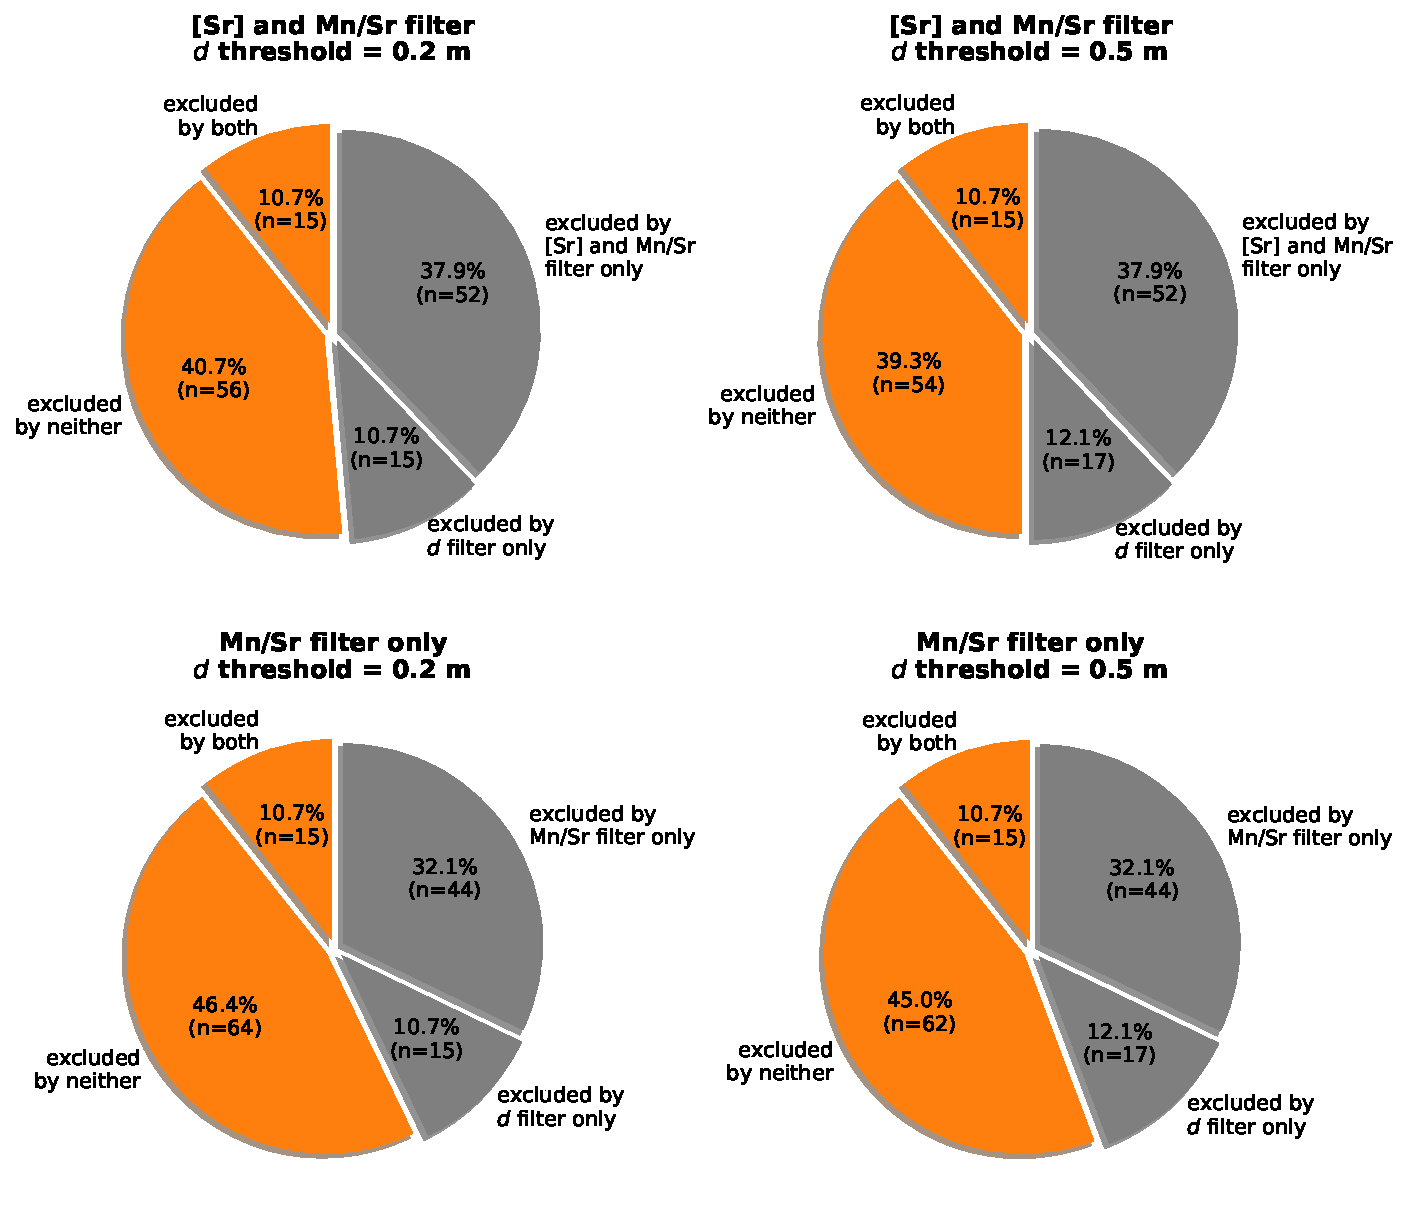
\includegraphics[width=0.8\textwidth]{figures/Tambien/filter-comparison.pdf}
	\caption{Comparison of the application of the [Sr] and Mn/Sr filter and the filter based on distance to siliciclastics (\dsil) to the \SrSr data, for both \dsil = 0.2~m and \dsil = 0.5~m. Orange sectors denote classification agreement between the two filters, and grey sectors denote classification disagreement between the two filters. In the upper row, both the [Sr] and Mn/Sr thresholds are combined to filter samples. In the lower row, only the Mn/Sr threshold is used to filter samples.}
	\label{fig:filter-comparison}
\end{center}
\end{figure}

Figure \ref{fig:filter-comparison} compares the application of the [Sr] and Mn/Sr filter and the filter based on distance to siliciclastics (\dsil) to the \SrSr data. When both the [Sr] and Mn/Sr thresholds are combined to filter samples (as in the main text), the [Sr] and Mn/Sr filter and the \dsil filter only agree on classification for around half of the samples. This lack of agreement results from the fact that the principal components analysis used for the \dsil filter (see main text) includes Mn/Sr, and not [Sr], as a variable in the analysis, since [Sr] in carbonates can vary considerably based on factors other than secondary alteration (e.g. calcite vs. aragonite, \citealp{Husson2015b}). Therefore, by using the Mn/Sr threshold only to filter samples, agreement between the Mn/Sr filter and the \dsil filter improves. Still, considerable disagreement between the two filters remain, which highlights the limitations of the \dsil filter as discussed in the main text. Namely, that in addition to filtering out samples that have been altered, it is a rather blunt filter and may also filter out samples that retain relatively pristine geochemistry.

\section{Pre-Sturtian \SrSr and the Drivers of Planetary Cooling}

\subsection{LIP Analysis}

\begin{sidewaystable*}
\scriptsize
\vspace*{1 cm}
\caption{Large igneous provinces included in the analysis conducted in the main text.}
\vspace{1 cm}
    \resizebox{\linewidth}{!}{
	\begin{tabular}{l l c c c l l l}
    \textbf{Name} & \textbf{Craton} & \textbf{Emplacement} & \textbf{Emplacement} & \textbf{Polygon Centroid} & \textbf{Age Reference} & \textbf{Polygon Reference} & \textbf{Paleomagnetic Pole} \\
    & & \textbf{Age [Ma]} & \textbf{Area [Mkm$^{2}$]} & \textbf{Emplacement Latitude} & & & \textbf{Reference} \\
    \hline \\ \vspace{0.2 cm}
    Mackenzie & Laurentia & 1267 & 2.983 & 11.4 & \citet{LeCheminant1989a} & \citet{Ernst2017a} & \citet{Buchan2000a} \\ \vspace{0.2 cm}
    CSDG & Baltica & 1255 & 0.145 & -24 & \citet{Soderlund2006a} & \citet{Ernst2017a} & \citet{Pisarevsky2014b} \\ \vspace{0.2 cm}
    Sudbury & Laurentia & 1235 & 0.056 & 7.7 & \citet{Dudas1994a} & \citet{Shellnutt2012a} & \citet{Palmer1977a} \\ \vspace{0.2 cm}
    Marnda Moorn & SW. Australia & 1210 & 0.598 & 65.2 & \citet{Pisarevsky2014a} & \citet{Ernst2017a} & \citet{Pisarevsky2014a} \\ \vspace{0.2 cm}
    Abitibi & Laurentia & 1141 & 0.229 & 48.2 & \citet{Krogh1987a} & \citet{Ernst2017a} & \citet{Ernst1993a} \\ \vspace{0.2 cm}
    Umkondo & Kalahari & 1109 & 1.846 & 0.8 & \citet{Hanson2004a} & \citet{Ernst2017a} & \citet{Swanson-Hysell2015b} \\ \vspace{0.2 cm}
    Keweenawan & Laurentia & 1109 & 0.414 & 41.9 & \citet{Davis1997a} & \citet{Ernst2017a} & \citet{Swanson-Hysell2014b} \\ \vspace{0.2 cm}
    SW Laurentia & Laurentia & 1090 & 0.776 & 28.7 & \citet{Weil2003a} & \citet{Bright2014a} & \citet{Weil2003a} \\ \vspace{0.2 cm}
    Warakurna - 1 & SW. + N. Australia & 1070 & 0.757 & 38.6 & \citet{Wingate2002a} & \citet{Ernst2017a} & \citet{Wingate2002a} \\ \vspace{0.2 cm}
    Warakurna - 2 & SW. + N. Australia & 1070 & 0.444 & 41.9 & \citet{Wingate2002a} & \citet{Ernst2017a} & \citet{Wingate2002a} \\ \vspace{0.2 cm}
    Dashigou & N. China & 925 & 0.663 & 3.9 & \citet{Peng2011a} & \citet{Pirajno2013a} & - \\ \vspace{0.2 cm}
    Gangil-Mayumbia & Congo & 920 & 0.333 & -52.3 & \citet{Tack2001a} & \citet{Ernst2017a} & - \\ \vspace{0.2 cm}
    Willouran-Gairdner - 1 & S. Australia & 827 & 0.345 & 24.3 & \citet{Wingate1998a} & \citet{Ernst2017a} & - \\ \vspace{0.2 cm}
    Willouran-Gairdner - 2 & S. Australia & 827 & 0.171 & 29.3 & \citet{Wingate1998a} & \citet{Ernst2017a} & - \\ \vspace{0.2 cm}
    SWCUC - 1 & S. China & 821 & 0.914 & 68.6 & \citet{Wang2016b} & \citet{Ernst2017a} & \citet{Li2004a} \\ \vspace{0.2 cm}
    SWCUC - 2 & S. China & 821 & 0.411 & 65.6 & \citet{Wang2016b} & \citet{Ernst2017a} & \citet{Li2004a} \\ \vspace{0.2 cm}
    Gunbarrel - 1 & Laurentia & 780 & 0.21 & -7 & \citet{Harlan2003a} & \citet{Ernst2017a} & \citet{Park1989a} \\ \vspace{0.2 cm}
    Gunbarrel - 2 & Laurentia & 780 & 0.34 & 4.2 & \citet{Harlan2003a} & \citet{Ernst2017a} & \citet{Park1989a} \\ \vspace{0.2 cm}
    Mundine Well & N. Australia & 755 & 0.21 & 25.6 & \citet{Wingate2000a} & \citet{Ernst2017a} & \citet{Wingate2000a} \\ \vspace{0.2 cm}
    Irkutsk & Siberia & 724 & 0.154 & 13.6 & \citet{Ernst2016a} & \citet{Ernst2016a} & - \\ \vspace{0.2 cm}
    Franklin & Laurentia & 720 & 2.231 & -2.3 & \citet{Denyszyn2009a} & \citet{Ernst2017a} & \citet{Denyszyn2009a} \\
    \hline
	\end{tabular}}
	
	\flushleft \emph{Notes:} \\
    LIPs \textgreater0.1~Mkm$^{2}$ from the compilation in \citep{Ernst2008a} were included in the LIP analysis in the main text. Some LIPs are comprised of two separate polygons (denoted by 1 and 2).
	\label{tab:LIPs}
\end{sidewaystable*}

Table \ref{tab:LIPs} lists the large igneous provinces (LIPs) that were included in the LIP analysis in the main text. The extent of each LIP was traced in QGIS to generate shapefiles, which were then added to a paleogeographic model \citep{Swanson-Hysell2019a} to extract the paleolatitude of the LIPs. We note that the LIP polygons were drawn to include the full areal extent of all dykes, sills, and volcanics interpreted to be associated with each LIP, which may lead to an overestimate of the true emplacement extents, since subsurface intrusions could extend over a broader area than the surface volcanics. Where available, the paleogeographic model honors the paleomagnetic poles listed in Table \ref{tab:LIPs}.

\subsection{Global Weathering Model}

The Python code used to develop the global weathering model can be found at: \url{https://github.com/Swanson-Hysell-Group/2019_Tambien_Group}. Table \ref{tab:seawater-model-variables} shows the variables and equations used in the global weathering model.

\begin{table}
\scriptsize
\vspace*{1 cm}
\caption{Variables used in the global weathering model.}
\vspace{1 cm}
\resizebox{\linewidth}{!}{
	\begin{tabular}{l l c}
	\textbf{Term} & \textbf{Value/Equation} & \textbf{Note} \\
	\hline
	\hline
	&&\\
	\textbf{Subaerial} & & \\
	\hline
	$[Ca]_{carb}$ & 302300~ppm & (1) \\
	$[Mg]_{carb}$ & 47000~ppm & (1) \\
	$[Sr]_{carb}$ & 610~ppm & (1) \\
	$[Ca]_{rad}$ & 23750~ppm & (2) \\
	$[Mg]_{rad}$ & 12800~ppm & (2) \\
	$[Sr]_{rad}$ & 310~ppm & (2) \\
	$[Ca]_{juv}$ & 71600~ppm & (3) \\
	$[Mg]_{juv}$ & 45500~ppm & (3) \\
	$[Sr]_{juv}$ & 465~ppm & (3) \\
	&&\\
	\textbf{Hydrothermal} & & \\
	\hline
	$H_{Mg-clays}$ & $k \cdot [Mg]$ & - \\
	$k$ & - & (4) \\
	$H_{Ca-basalt}$ & $\alpha_{Mg/Ca} \cdot H_{Mg-clays}$ & - \\
	$\alpha_{Mg/Ca}$ & 1 & (5) \\
	$H_{^{n}Sr-basalt}$ & $\alpha_{Sr/Ca} \cdot H_{Ca-basalt}$ & - \\
	$\alpha_{Sr/Ca}$ & 0.0013 & (6) \\
	&&\\
	\textbf{Precipitation} & & \\
	\hline
	$P_{Ca-carb}$ & $W_{Mg-carb}+W_{Mg-rad}+W_{Mg-juv}-P_{Mg-carb}+W_{Ca-carb}+W_{Ca-rad}+W_{Ca-juv}$ & (7) \\
	$P_{Mg-carb}$ & $5\times10^{10}$~mol/yr & (8) \\
	$P_{Sr-carb}$ & $(Sr/Ca)_{seawater} \cdot K_{Sr} \cdot P_{Ca-carb}$ & - \\
	$K_{Sr}$ & 0.2 & (9) \\
	&&\\
	\textbf{\SrSr} & & \\
	\hline
	carbonate & 0.70475 & (10) \\
	radiogenic & $BABI+(0.2783\left(\frac{Rb}{Sr}\right)_{m}(9.3485+BABI))(1-e^{-2\times10^{9}\lambda})+$ & (11) \\
	& $10(0.2783\left(\frac{Rb}{Sr}\right)_{m}(9.3485+BABI))(1-e^{-\lambda(t-2\times10^{9})})$ & \\
	juvenile & $BABI+(0.2783\left(\frac{Rb}{Sr}\right)_{m}(9.3485+BABI))(1-e^{-\lambda t})$ & (11) \\
	\hline
	\end{tabular}}
	
	\flushleft \emph{Notes:} \\
    (1) from \citet{Turekian1961a}\\
    (2) from \citet{Wedepohl1995a}\\
    (3) taking the mean of \citet{Turekian1961a} and \citet{Taylor1964a}\\
    (4) flux of H$_{2}$O in hydrothermal systems, estimated to achieve desired initial steady state, then varied\\
    (5) assumes 1:1 stoichiometry between Mg and Ca during weathering of the ocean crust\\
    (6) from \citet{Maloof2010a}, calculated assuming 200~ppm Sr and 10~wt\% CaO\\
    (7) calculated iteratively assuming carbonate minerals are the only Ca sink\\
    (8) estimated to achieve desired initial steady state\\
    (9) homogeneous distribution coefficient for Sr in calcite from \citet{Mucci1983a}\\
    (10) seawater has roughly constant \SrSr $\sim$2-1~Ga \citep{Shields2002a}\\
    (11) these equations account of $^{87}$Rb decay, where $BABI$ is the Basaltic Achondrite Best Initial ratio (\SrSr=0.69897) from \citet{Papanastassiou1968a}, $\left(\frac{Rb}{Sr}\right)_{m}$ is Rb/Sr of the mantle (0.025), $\lambda$ is the $^{87}$Rb decay constant, and $t$ is time since the origin of the Earth.
	\label{tab:seawater-model-variables}
\end{table}
\chapter[Supporting Information for ``Tonian paleomagnetism from South China permits an inclusive Rodinia or Bitter Springs Stage true polar wander, but not both''][Supporting Information - Xiajiang Group]{Supporting Information for ``Tonian paleomagnetism from South China permits an inclusive Rodinia or Bitter Springs Stage true polar wander, but not both''}

\begin{figure}[h!]
    \centering
    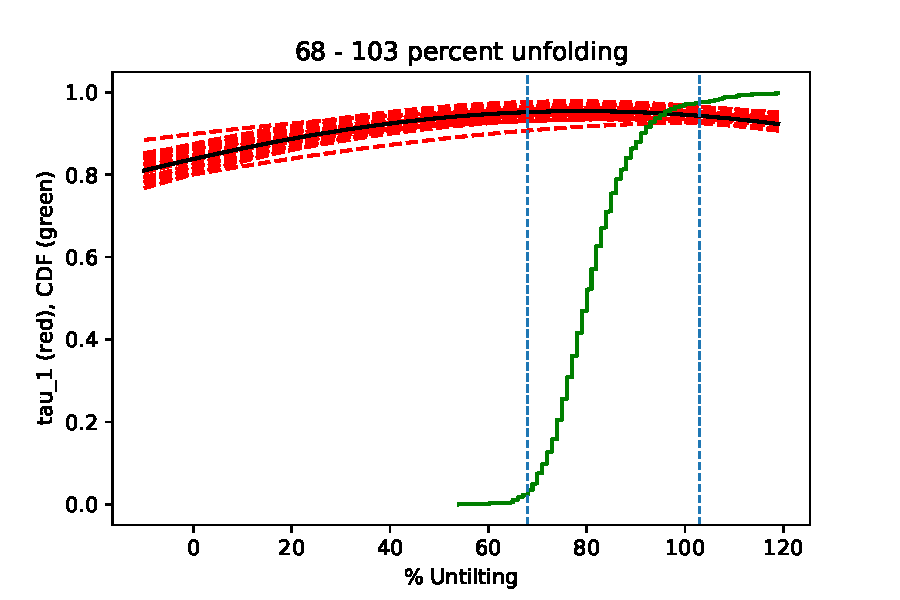
\includegraphics[width=0.8\textwidth]{figures/Xiajiang/bootstrap-CDF.pdf}
    \caption[Results of the bootstrap fold test for the Xiajiang Group high-temperature component.]{Results of the bootstrap fold test \citep{Tauxe1994a} for the Xiajiang Group high-temperature component. The tightest grouping of site mean directions is obtained between 68 and 103\% unfolding at the 95\% confidence level. Since this range encompasses 100\%, the high-temperature component passes the fold test, constraining the high-temperature component to have been acquired prior to Mesozoic folding of the Xiajiang Group \citep{Li2016c, Ma2019a}.}
    \label{fig:bootstrap-CDF}
\end{figure}

\begin{figure}[h!]
    \centering
    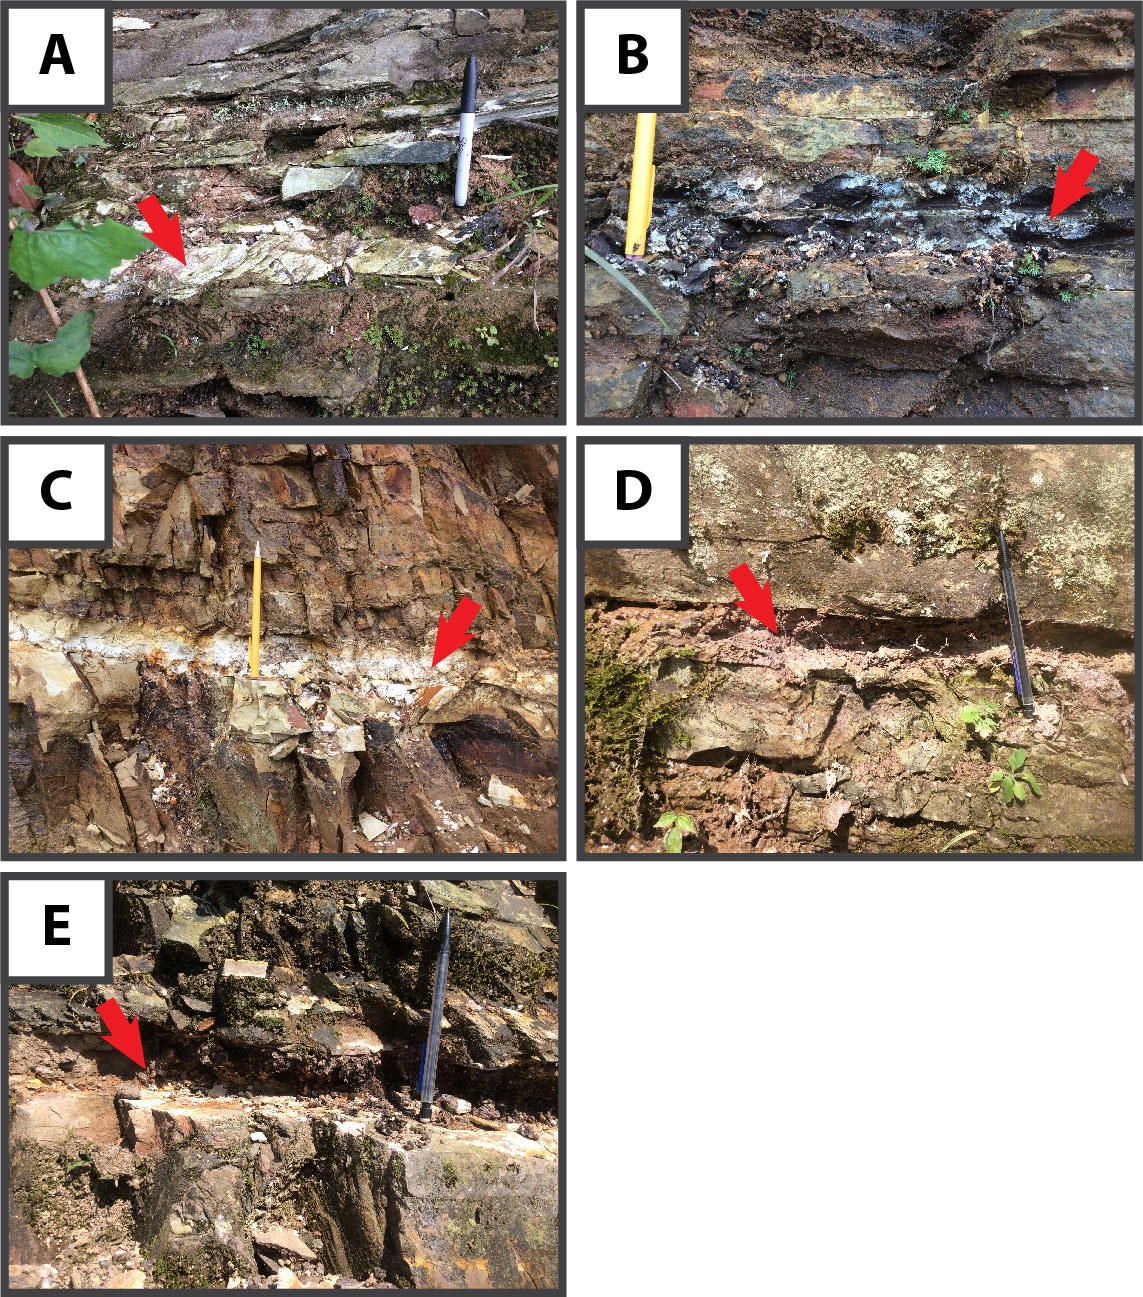
\includegraphics[width=0.9\textwidth]{figures/Xiajiang/tuff-photos.jpg}
    \caption[Photographs of tuffs in the Xiajiang Group.]{Photographs of tuffs that yielded consistent and concordant CA-ID-TIMS $^{206}$Pb/$^{238}$U zircon dates. Red arrows point to the sampled tuffs. \textbf{A)} H2-470. \textbf{B)} H3-60. \textbf{C)} H3-8. \textbf{D)} QR-74. \textbf{E)} L4-2. No photograph is available for sample L1-27.}
    \label{fig:tuff-photos}
\end{figure}

\begin{figure}[h!]
    \centering
    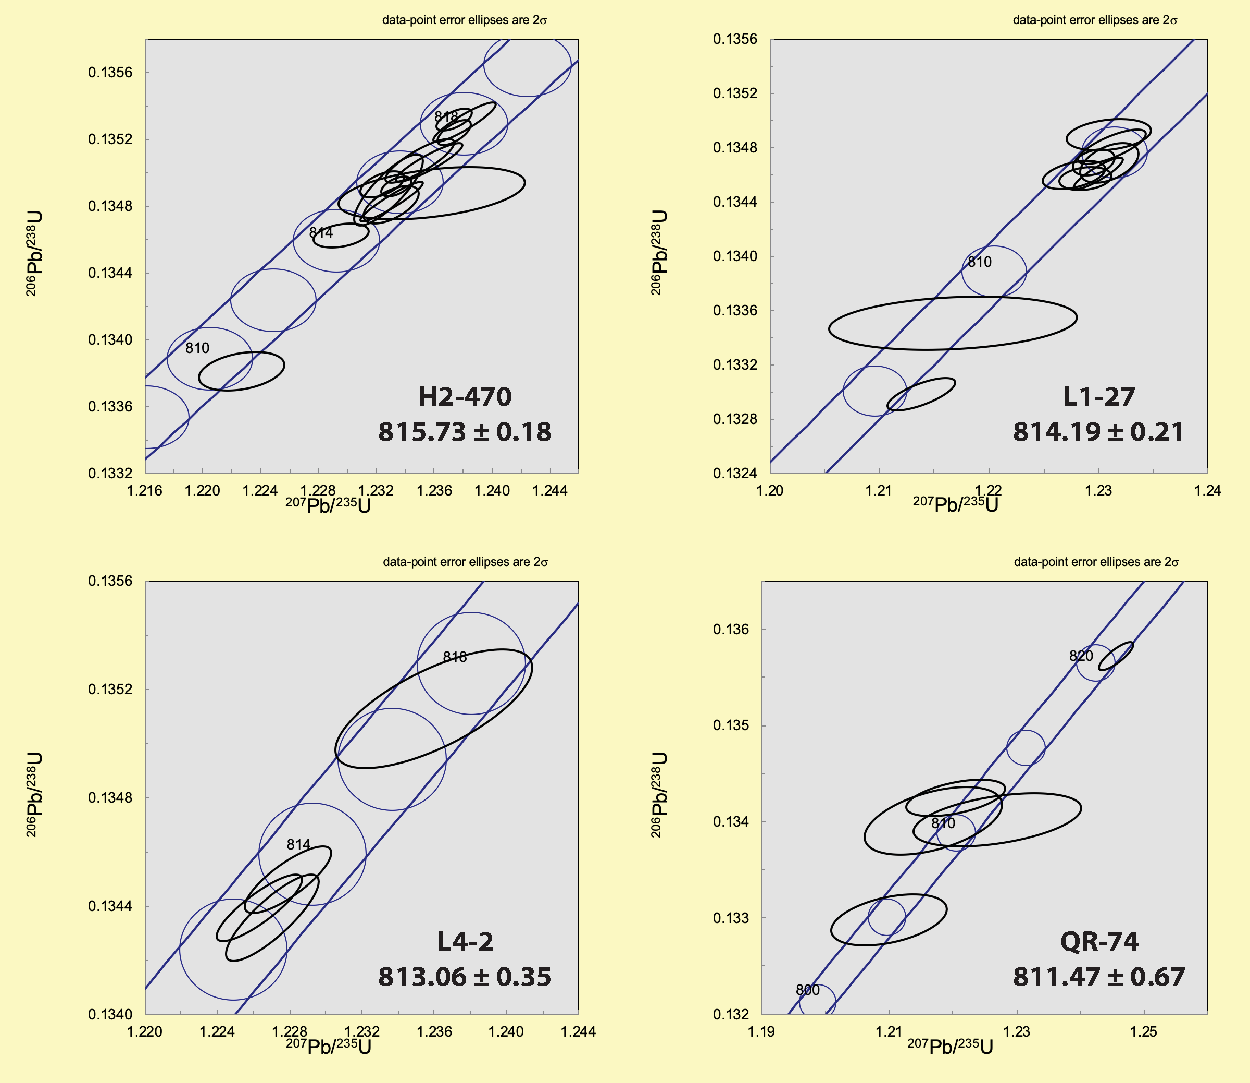
\includegraphics[width=0.9\textwidth]{figures/Xiajiang/concordia-1.pdf}
    \caption[Concordia diagrams for zircons from tuffs of the Xiajiang Group.]{Concordia diagrams for zircons from tuffs of the Xiajiang Group analyzed in this study. Individual zircon data are tabulated in Table SX.}
    \label{fig:concordia-1}
\end{figure}

\begin{figure}[h!]
    \centering
    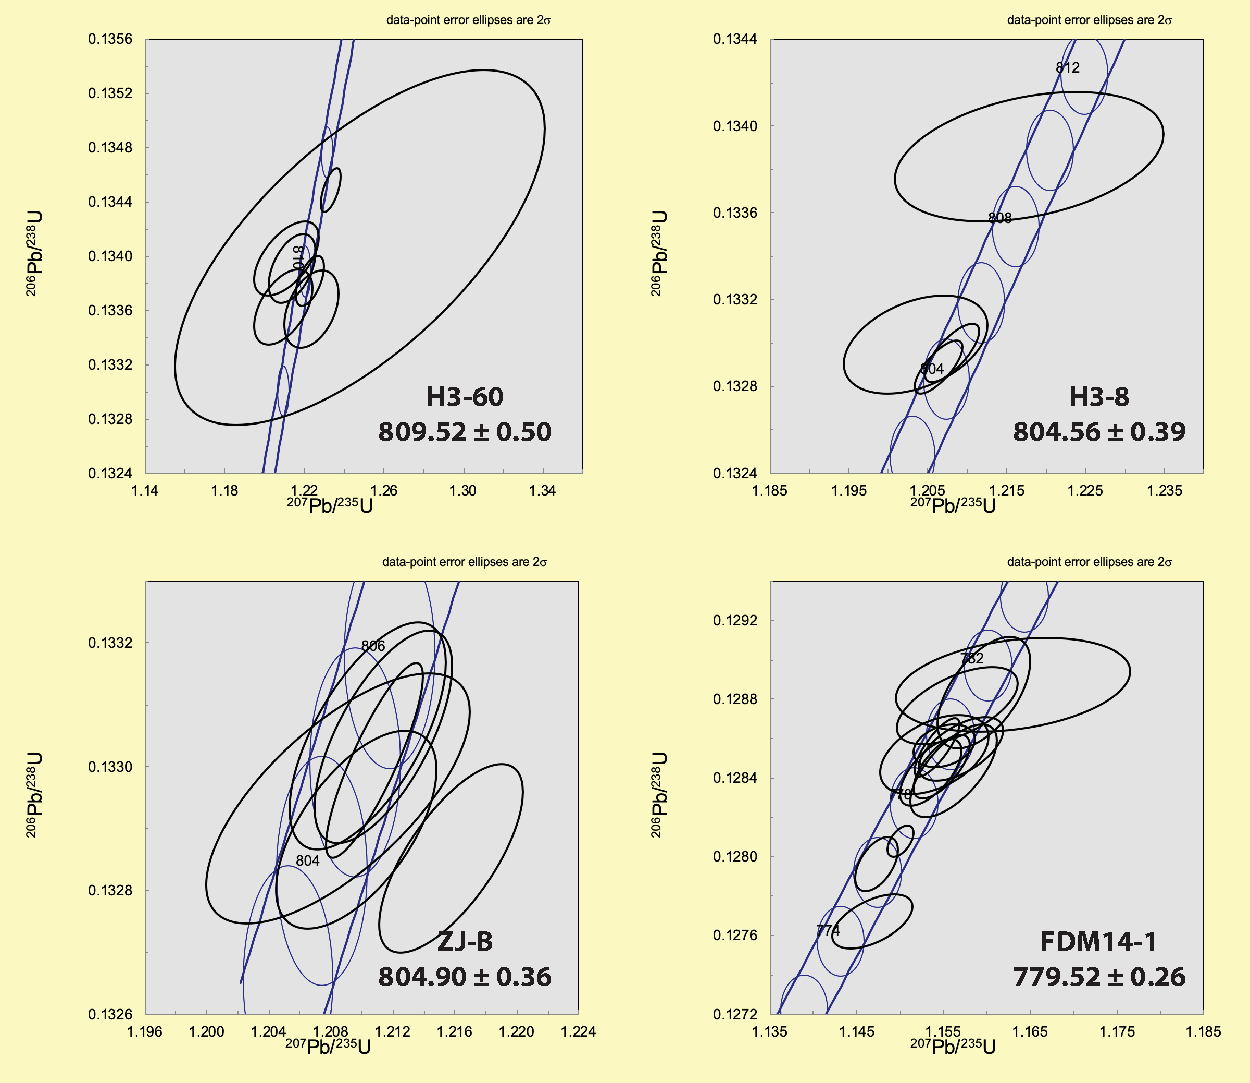
\includegraphics[width=0.9\textwidth]{figures/Xiajiang/concordia-2.pdf}
    \caption[Concordia diagrams for zircons from tuffs of the Xiajiang Group, Madiyi Formation, and Liantuo Formation.]{Concordia diagrams for zircons from tuffs of the Xiajiang Group (H3-60 and H3-8), Madiyi Formation (ZJ-B), and Liantuo Formation (FDM14-1) analyzed in this study. Individual zircon data are tabulated in Table SX.}
    \label{fig:concordia-2}
\end{figure}

\begin{figure}[h!]
    \centering
    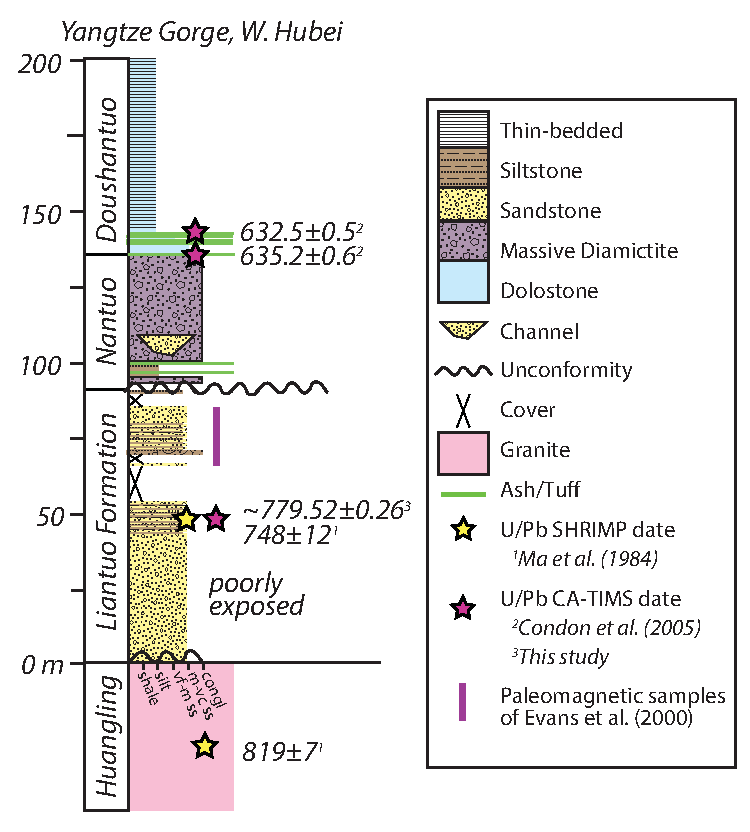
\includegraphics[width=0.8\textwidth]{figures/Xiajiang/FDM14-1-strat.pdf}
    \caption[Tonian-Cryogenian stratigraphy of the Yangtze Gorge.]{Tonian-Cryogenian stratigraphy of the Yangtze Gorge, from where the paleomagnetic and geochronologic data for the Liantuo Formation are developed.}
    \label{fig:FDM14-1-strat}
\end{figure}

\begin{sidewaystable*}[h!]
\tiny
\vspace*{1 cm}
\caption{U-Pb data for analyzed zircons from H2-470.}
\vspace{1 cm}
\setlength\tabcolsep{3.5pt}
\begin{tabular}{cccccccccccccccccccc}
& \multicolumn{8}{l}{Dates (Ma)} & \multicolumn{4}{l}{Composition} & \multicolumn{7}{l}{Isotopic Ratios} \\
\cline{2-20}\\
& $^a$ & & $^b$ & & $^{a,b}$ & & & $^c$ & $^d$ & $^e$ & $^f$ & $^{g}$ & $^h$ & $^{a,i}$ & & $^{b,i}$ & & $^{a,b,i}$ & \\	
& \underline{$^{206}$Pb} & $\pm$ & \underline{$^{207}$Pb} & $\pm$ & \underline{$^{207}$Pb} & $\pm$ & corr. & & \underline{Th} & Pb\** & Pb$_c$ & \underline{Pb\**} & \underline{$^{206}$Pb} & \underline{$^{206}$Pb} & $\pm$ & \underline{$^{207}$Pb} & $\pm$ & \underline{$^{207}$Pb} & $\pm$ \\		
fraction & $^{238}$U & (2$\sigma$) & $^{235}$U & (2$\sigma$) & $^{206}$Pb & (2$\sigma$) & coef. & \% disc. & U & (pg) & (pg) & Pb$_c$ & $^{204}$Pb & $^{238}$Pb & (2$\sigma\%$) & $^{235}$U & (2$\sigma\%$) & $^{206}$Pb & (2$\sigma\%$) \\
\hline \\
z9  & 809.55 & 0.53 & 811.00 & 1.10 & 814.95 & 3.88 & 0.33 & 0.69  & 0.90 & 15.6  & 0.25 & 62.2   & 3392  & 0.133808 & 0.070220 & 1.222669 & 0.196189 & 0.066301 & 0.182537 \\
z11 & 814.18 & 0.34 & 814.14 & 0.70 & 814.03 & 2.46 & 0.34 & 0.01  & 0.74 & 24.5  & 0.17 & 141.8  & 7993  & 0.134622 & 0.044107 & 1.229565 & 0.125086 & 0.066272 & 0.113043 \\
\rowcolor{Yellow}
z14 & 815.23 & 0.52 & 815.70 & 0.71 & 816.99 & 2.14 & 0.59 & 0.25  & 0.77 & 151.5 & 0.32 & 479.9  & 26838 & 0.134807 & 0.067705 & 1.232995 & 0.126378 & 0.066366 & 0.096844 \\
\rowcolor{Yellow}
z2  & 815.35 & 0.54 & 815.71 & 0.80 & 816.70 & 1.69 & 0.93 & 0.20  & 0.58 & 181.3 & 0.18 & 1013.2 & 59304 & 0.134828 & 0.070797 & 1.233019 & 0.143199 & 0.066356 & 0.074214 \\
\rowcolor{Yellow}
z3  & 815.62 & 0.72 & 816.98 & 2.39 & 820.70 & 8.28 & 0.41 & 0.65  & 0.62 & 95.6  & 5.15 & 18.6   & 1093  & 0.134876 & 0.093966 & 1.235816 & 0.424989 & 0.066484 & 0.394981 \\
\rowcolor{Yellow}
z7  & 815.73 & 0.99 & 815.63 & 0.88 & 815.35 & 1.90 & 0.82 & -0.02 & 0.88 & 38.7  & 0.30 & 128.9  & 7036  & 0.134895 & 0.128998 & 1.232832 & 0.157563 & 0.066314 & 0.084703 \\
\rowcolor{Yellow}
z8  & 815.85 & 0.27 & 815.87 & 0.40 & 815.92 & 1.25 & 0.53 & 0.04  & 0.72 & 35.1  & 0.15 & 226.9  & 12842 & 0.134917 & 0.035031 & 1.233366 & 0.070632 & 0.066332 & 0.050324 \\
\rowcolor{Yellow}
z12 & 815.93 & 0.36 & 815.43 & 0.56 & 814.06 & 1.78 & 0.54 & -0.20 & 0.78 & 23.6  & 0.16 & 148.4  & 8295  & 0.134931 & 0.047158 & 1.232398 & 0.100758 & 0.066273 & 0.078418 \\
z1  & 816.69 & 0.53 & 816.90 & 0.84 & 817.48 & 1.95 & 0.90 & 0.13  & 0.76 & 132.2 & 0.74 & 179.4  & 10069 & 0.135064 & 0.069554 & 1.235639 & 0.150465 & 0.066381 & 0.087256 \\
z4  & 816.73 & 0.61 & 816.60 & 0.88 & 816.24 & 2.11 & 0.83 & -0.03 & 0.73 & 32.6  & 0.12 & 272.7  & 15417 & 0.135072 & 0.079228 & 1.234975 & 0.156380 & 0.066342 & 0.095355 \\
z6  & 817.69 & 0.34 & 817.70 & 0.42 & 817.73 & 1.19 & 0.65 & 0.04  & 0.86 & 60.2  & 0.26 & 232.1  & 12723 & 0.135239 & 0.044110 & 1.237385 & 0.074873 & 0.066389 & 0.046714 \\
z5  & 818.04 & 0.54 & 818.01 & 0.80 & 817.92 & 1.78 & 0.90 & 0.02  & 0.72 & 57.6  & 0.14 & 408.6  & 23141 & 0.135301 & 0.070555 & 1.238068 & 0.143195 & 0.066395 & 0.078665 \\
z10 & 818.13 & 0.30 & 817.69 & 0.44 & 816.47 & 1.32 & 0.62 & -0.17 & 0.76 & 50.0  & 0.16 & 311.7  & 17475 & 0.135318 & 0.038917 & 1.237363 & 0.079176 & 0.066349 & 0.053969 \\
z16 & 826.68 & 0.32 & 824.61 & 0.43 & 819.04 & 1.27 & 0.61 & -0.90 & 0.74 & 93.5  & 0.30 & 311.7  & 17581 & 0.136824 & 0.040989 & 1.252669 & 0.076810 & 0.066431 & 0.051484 \\
z13 & 830.20 & 0.53 & 825.34 & 0.85 & 812.27 & 2.03 & 0.87 & -2.17 & 0.75 & 62.5  & 0.38 & 164.3  & 9250  & 0.137445 & 0.068375 & 1.254296 & 0.149999 & 0.066216 & 0.091207 \\
z15 & 844.63 & 0.31 & 837.47 & 0.90 & 818.55 & 3.17 & 0.28 & -3.16 & 1.03 & 41.3  & 0.76 & 54.4   & 2879  & 0.139994 & 0.038917 & 1.281393 & 0.158093 & 0.066415 & 0.148349 \\
\end{tabular}

\flushleft \emph{Notes:} \\
Colored rows indicate fractions included in the calculation of the reported sample age. \\
Isotopic dates calculated using $\lambda$238 = 1.55125$\times$10$^{-10}$ and $\lambda$235 = 9.8485$\times$10$^{-10}$ \citep{Jaffey1971a}. \\
 $^{a}$  Corrected for initial Th/U disequilibrium using radiogenic $^{208}$Pb and Th/U[magma] = 2.8. \\
 $^{b}$ Corrected for initial Pa/U disequilibrium using initial fraction activity ratio [$^{231}$Pa]/[$^{235}$U] = 1.10000. \\
 $^{c}$ \% discordance = 100 - (100 $\times$ ($^{206}$Pb/$^{238}$U date) / ($^{207}$Pb/$^{206}$Pb date)) \\
 $^{d}$ Th contents calculated from radiogenic $^{208}$Pb and $^{230}$Th-corrected $^{206}$Pb/$^{238}$U date of the sample, assuming concordance between U-Pb Th-Pb systems. \\
 $^{e}$ Total mass of radiogenic Pb. \\
 $^{f}$ Total mass of common Pb. \\
 $^{g}$ Ratio of radiogenic Pb (including $^{208}$Pb) to common Pb. \\
 $^{h}$ Measured ratio corrected for fractionation and spike contribution only. \\
 $^{i}$ Measured ratios corrected for fractionation, tracer and blank.
\end{sidewaystable*}

\begin{sidewaystable*}[h!]
\tiny
\vspace*{1 cm}
\caption{U-Pb data for analyzed zircons from L1-27.}
\vspace{1 cm}
\setlength\tabcolsep{3.5pt}
\begin{tabular}{cccccccccccccccccccc}
& \multicolumn{8}{l}{Dates (Ma)} & \multicolumn{4}{l}{Composition} & \multicolumn{7}{l}{Isotopic Ratios} \\
\cline{2-20}\\
& $^a$ & & $^b$ & & $^{a,b}$ & & & $^c$ & $^d$ & $^e$ & $^f$ & $^{g}$ & $^h$ & $^{a,i}$ & & $^{b,i}$ & & $^{a,b,i}$ & \\	
& \underline{$^{206}$Pb} & $\pm$ & \underline{$^{207}$Pb} & $\pm$ & \underline{$^{207}$Pb} & $\pm$ & corr. & & \underline{Th} & Pb\** & Pb$_c$ & \underline{Pb\**} & \underline{$^{206}$Pb} & \underline{$^{206}$Pb} & $\pm$ & \underline{$^{207}$Pb} & $\pm$ & \underline{$^{207}$Pb} & $\pm$ \\		
fraction & $^{238}$U & (2$\sigma$) & $^{235}$U & (2$\sigma$) & $^{206}$Pb & (2$\sigma$) & coef. & \% disc. & U & (pg) & (pg) & Pb$_c$ & $^{204}$Pb & $^{238}$Pb & (2$\sigma\%$) & $^{235}$U & (2$\sigma\%$) & $^{206}$Pb & (2$\sigma\%$) \\
\hline \\
z5  & 804.84 & 0.56 & 806.95 & 1.16 & 812.78 & 3.42  & 0.72 & 1.01  & 0.73 & 50.5 & 0.82 & 61.7  & 3500 & 0.132980 & 0.073384 & 1.213839 & 0.207803 & 0.066232 & 0.160083 \\
z6  & 807.82 & 0.91 & 808.27 & 4.24 & 809.52 & 15.58 & 0.22 & 0.24  & 0.79 & 7.0  & 0.63 & 11.1  & 638  & 0.133504 & 0.119942 & 1.216721 & 0.761579 & 0.066129 & 0.744112 \\
\rowcolor{Yellow}
z9  & 813.90 & 0.39 & 813.80 & 0.88 & 813.52 & 3.20  & 0.22 & -0.02 & 0.85 & 27.2 & 0.32 & 85.4  & 4697 & 0.134572 & 0.050696 & 1.228808 & 0.156387 & 0.066256 & 0.149699 \\
\rowcolor{Yellow}
z8  & 814.06 & 0.48 & 813.32 & 1.08 & 811.29 & 3.66  & 0.43 & -0.31 & 0.98 & 16.3 & 0.31 & 52.0  & 2787 & 0.134600 & 0.062729 & 1.227755 & 0.192831 & 0.066185 & 0.172067 \\
\rowcolor{Yellow}
z2  & 814.11 & 0.53 & 814.33 & 0.83 & 814.92 & 1.97  & 0.88 & 0.13  & 0.62 & 55.9 & 0.33 & 169.6 & 9852 & 0.134610 & 0.068803 & 1.229970 & 0.148922 & 0.066300 & 0.088455 \\
\rowcolor{Yellow}
z12 & 814.55 & 0.67 & 814.81 & 0.99 & 815.50 & 3.29  & 0.46 & 0.14  & 1.10 & 18.0 & 0.26 & 68.8  & 3583 & 0.134688 & 0.087437 & 1.231029 & 0.177274 & 0.066318 & 0.153859 \\
\rowcolor{Yellow}
z11 & 814.57 & 0.44 & 814.14 & 0.70 & 812.95 & 2.47  & 0.35 & -0.17 & 0.87 & 19.5 & 0.23 & 86.0  & 4714 & 0.134691 & 0.058009 & 1.229554 & 0.125152 & 0.066238 & 0.113683 \\
z4  & 815.24 & 0.59 & 814.91 & 1.15 & 814.02 & 3.28  & 0.75 & -0.12 & 0.84 & 18.9 & 0.27 & 71.1  & 3926 & 0.134808 & 0.076864 & 1.231253 & 0.205803 & 0.066271 & 0.153331 \\
z7  & 815.75 & 0.53 & 814.78 & 1.43 & 812.13 & 5.12  & 0.27 & -0.41 & 0.88 & 9.1  & 0.27 & 33.0  & 1818 & 0.134898 & 0.069355 & 1.230966 & 0.254447 & 0.066212 & 0.242857 \\
\end{tabular}

\flushleft \emph{Notes:} \\
Colored rows indicate fractions included in the calculation of the reported sample age. \\
Isotopic dates calculated using $\lambda$238 = 1.55125$\times$10$^{-10}$ and $\lambda$235 = 9.8485$\times$10$^{-10}$ \citep{Jaffey1971a}. \\
 $^{a}$  Corrected for initial Th/U disequilibrium using radiogenic $^{208}$Pb and Th/U[magma] = 2.8. \\
 $^{b}$ Corrected for initial Pa/U disequilibrium using initial fraction activity ratio [$^{231}$Pa]/[$^{235}$U] = 1.10000. \\
 $^{c}$ \% discordance = 100 - (100 $\times$ ($^{206}$Pb/$^{238}$U date) / ($^{207}$Pb/$^{206}$Pb date)) \\
 $^{d}$ Th contents calculated from radiogenic $^{208}$Pb and $^{230}$Th-corrected $^{206}$Pb/$^{238}$U date of the sample, assuming concordance between U-Pb Th-Pb systems. \\
 $^{e}$ Total mass of radiogenic Pb. \\
 $^{f}$ Total mass of common Pb. \\
 $^{g}$ Ratio of radiogenic Pb (including $^{208}$Pb) to common Pb. \\
 $^{h}$ Measured ratio corrected for fractionation and spike contribution only. \\
 $^{i}$ Measured ratios corrected for fractionation, tracer and blank.
\end{sidewaystable*}

\begin{sidewaystable*}[h!]
\tiny
\vspace*{1 cm}
\caption{U-Pb data for analyzed zircons from L4-2.}
\vspace{1 cm}
\setlength\tabcolsep{3.5pt}
\begin{tabular}{cccccccccccccccccccc}
& \multicolumn{8}{l}{Dates (Ma)} & \multicolumn{4}{l}{Composition} & \multicolumn{7}{l}{Isotopic Ratios} \\
\cline{2-20}\\
& $^a$ & & $^b$ & & $^{a,b}$ & & & $^c$ & $^d$ & $^e$ & $^f$ & $^{g}$ & $^h$ & $^{a,i}$ & & $^{b,i}$ & & $^{a,b,i}$ & \\	
& \underline{$^{206}$Pb} & $\pm$ & \underline{$^{207}$Pb} & $\pm$ & \underline{$^{207}$Pb} & $\pm$ & corr. & & \underline{Th} & Pb\** & Pb$_c$ & \underline{Pb\**} & \underline{$^{206}$Pb} & \underline{$^{206}$Pb} & $\pm$ & \underline{$^{207}$Pb} & $\pm$ & \underline{$^{207}$Pb} & $\pm$ \\		
fraction & $^{238}$U & (2$\sigma$) & $^{235}$U & (2$\sigma$) & $^{206}$Pb & (2$\sigma$) & coef. & \% disc. & U & (pg) & (pg) & Pb$_c$ & $^{204}$Pb & $^{238}$Pb & (2$\sigma\%$) & $^{235}$U & (2$\sigma\%$) & $^{206}$Pb & (2$\sigma\%$) \\
\hline \\
\rowcolor{Yellow}
z5 & 812.67 & 0.73 & 812.99 & 0.96 & 813.86 & 2.20 & 0.84 & 0.18  & 0.64 & 28.3 & 0.17 & 170.0 & 9812 & 0.134357 & 0.096183 & 1.227035 & 0.171839 & 0.066266 & 0.100134 \\
\rowcolor{Yellow}
z3 & 812.88 & 0.57 & 812.67 & 0.88 & 812.09 & 2.13 & 0.85 & -0.07 & 0.76 & 96.5 & 0.70 & 137.1 & 7703 & 0.134393 & 0.074304 & 1.226330 & 0.157528 & 0.066210 & 0.096556 \\
\rowcolor{Yellow}
z1 & 813.47 & 0.57 & 813.40 & 0.89 & 813.19 & 2.27 & 0.81 & 0.00  & 0.79 & 72.4 & 0.46 & 157.4 & 8784 & 0.134497 & 0.074341 & 1.227932 & 0.159174 & 0.066245 & 0.103450 \\
z4 & 817.05 & 1.02 & 817.05 & 2.02 & 817.07 & 5.95 & 0.70 & 0.03  & 0.78 & 10.7 & 0.25 & 43.5  & 2442 & 0.135127 & 0.132953 & 1.235972 & 0.360619 & 0.066368 & 0.282745 \\
\end{tabular}

\flushleft \emph{Notes:} \\
Colored rows indicate fractions included in the calculation of the reported sample age. \\
Isotopic dates calculated using $\lambda$238 = 1.55125$\times$10$^{-10}$ and $\lambda$235 = 9.8485$\times$10$^{-10}$ \citep{Jaffey1971a}. \\
 $^{a}$  Corrected for initial Th/U disequilibrium using radiogenic $^{208}$Pb and Th/U[magma] = 2.8. \\
 $^{b}$ Corrected for initial Pa/U disequilibrium using initial fraction activity ratio [$^{231}$Pa]/[$^{235}$U] = 1.10000. \\
 $^{c}$ \% discordance = 100 - (100 $\times$ ($^{206}$Pb/$^{238}$U date) / ($^{207}$Pb/$^{206}$Pb date)) \\
 $^{d}$ Th contents calculated from radiogenic $^{208}$Pb and $^{230}$Th-corrected $^{206}$Pb/$^{238}$U date of the sample, assuming concordance between U-Pb Th-Pb systems. \\
 $^{e}$ Total mass of radiogenic Pb. \\
 $^{f}$ Total mass of common Pb. \\
 $^{g}$ Ratio of radiogenic Pb (including $^{208}$Pb) to common Pb. \\
 $^{h}$ Measured ratio corrected for fractionation and spike contribution only. \\
 $^{i}$ Measured ratios corrected for fractionation, tracer and blank.
\end{sidewaystable*}

\begin{sidewaystable*}[h!]
\tiny
\vspace*{1 cm}
\caption{U-Pb data for analyzed zircons from QR-74.}
\vspace{1 cm}
\setlength\tabcolsep{3.5pt}
\begin{tabular}{cccccccccccccccccccc}
& \multicolumn{8}{l}{Dates (Ma)} & \multicolumn{4}{l}{Composition} & \multicolumn{7}{l}{Isotopic Ratios} \\
\cline{2-20}\\
& $^a$ & & $^b$ & & $^{a,b}$ & & & $^c$ & $^d$ & $^e$ & $^f$ & $^{g}$ & $^h$ & $^{a,i}$ & & $^{b,i}$ & & $^{a,b,i}$ & \\	
& \underline{$^{206}$Pb} & $\pm$ & \underline{$^{207}$Pb} & $\pm$ & \underline{$^{207}$Pb} & $\pm$ & corr. & & \underline{Th} & Pb\** & Pb$_c$ & \underline{Pb\**} & \underline{$^{206}$Pb} & \underline{$^{206}$Pb} & $\pm$ & \underline{$^{207}$Pb} & $\pm$ & \underline{$^{207}$Pb} & $\pm$ \\		
fraction & $^{238}$U & (2$\sigma$) & $^{235}$U & (2$\sigma$) & $^{206}$Pb & (2$\sigma$) & coef. & \% disc. & U & (pg) & (pg) & Pb$_c$ & $^{204}$Pb & $^{238}$Pb & (2$\sigma\%$) & $^{235}$U & (2$\sigma\%$) & $^{206}$Pb & (2$\sigma\%$) \\
\hline \\
z3  & 804.83 & 1.24 & 805.14 & 3.41  & 806.01 & 11.84 & 0.42 & 0.17  & 1.23 & 22.8 & 1.33 & 17.1  & 879  & 0.132978 & 0.163397 & 1.209897 & 0.614028 & 0.066018 & 0.564721 \\
\rowcolor{Yellow}
z16 & 810.71 & 1.64 & 808.35 & 4.05  & 801.85 & 13.64 & 0.48 & -1.08 & 1.51 & 4.5  & 0.27 & 16.9  & 821  & 0.134012 & 0.215638 & 1.216885 & 0.726288 & 0.065887 & 0.650260 \\
\rowcolor{Yellow}
z11 & 810.75 & 1.28 & 812.97 & 4.90  & 819.06 & 17.07 & 0.44 & 1.02  & 2.16 & 4.4  & 0.29 & 15.3  & 661  & 0.134018 & 0.168352 & 1.226995 & 0.876654 & 0.066431 & 0.816287 \\
\rowcolor{Yellow}
z2  & 812.05 & 0.90 & 809.95 & 2.91  & 804.18 & 9.90  & 0.51 & -0.95 & 0.78 & 6.1  & 0.23 & 26.3  & 1483 & 0.134247 & 0.117602 & 1.220376 & 0.521619 & 0.065960 & 0.471892 \\
z8  & 820.43 & 0.67 & 821.41 & 1.00  & 824.08 & 2.43  & 0.82 & 0.48  & 0.53 & 51.0 & 0.34 & 151.9 & 9025 & 0.135722 & 0.086584 & 1.245585 & 0.176779 & 0.066591 & 0.111640 \\
z12 & 851.34 & 3.08 & 860.05 & 15.02 & 882.58 & 52.25 & 0.23 & 3.57  & 0.82 & 4.8  & 1.62 & 3.0   & 182  & 0.141182 & 0.386791 & 1.332696 & 2.588865 & 0.068493 & 2.526201 \\
\end{tabular}

\flushleft \emph{Notes:} \\
Colored rows indicate fractions included in the calculation of the reported sample age. \\
Isotopic dates calculated using $\lambda$238 = 1.55125$\times$10$^{-10}$ and $\lambda$235 = 9.8485$\times$10$^{-10}$ \citep{Jaffey1971a}. \\
 $^{a}$  Corrected for initial Th/U disequilibrium using radiogenic $^{208}$Pb and Th/U[magma] = 2.8. \\
 $^{b}$ Corrected for initial Pa/U disequilibrium using initial fraction activity ratio [$^{231}$Pa]/[$^{235}$U] = 1.10000. \\
 $^{c}$ \% discordance = 100 - (100 $\times$ ($^{206}$Pb/$^{238}$U date) / ($^{207}$Pb/$^{206}$Pb date)) \\
 $^{d}$ Th contents calculated from radiogenic $^{208}$Pb and $^{230}$Th-corrected $^{206}$Pb/$^{238}$U date of the sample, assuming concordance between U-Pb Th-Pb systems. \\
 $^{e}$ Total mass of radiogenic Pb. \\
 $^{f}$ Total mass of common Pb. \\
 $^{g}$ Ratio of radiogenic Pb (including $^{208}$Pb) to common Pb. \\
 $^{h}$ Measured ratio corrected for fractionation and spike contribution only. \\
 $^{i}$ Measured ratios corrected for fractionation, tracer and blank.
\end{sidewaystable*}

\begin{sidewaystable*}[h!]
\tiny
\vspace*{1 cm}
\caption{U-Pb data for analyzed zircons from H3-60.}
\vspace{1 cm}
\setlength\tabcolsep{3.5pt}
\begin{tabular}{cccccccccccccccccccc}
& \multicolumn{8}{l}{Dates (Ma)} & \multicolumn{4}{l}{Composition} & \multicolumn{7}{l}{Isotopic Ratios} \\
\cline{2-20}\\
& $^a$ & & $^b$ & & $^{a,b}$ & & & $^c$ & $^d$ & $^e$ & $^f$ & $^{g}$ & $^h$ & $^{a,i}$ & & $^{b,i}$ & & $^{a,b,i}$ & \\	
& \underline{$^{206}$Pb} & $\pm$ & \underline{$^{207}$Pb} & $\pm$ & \underline{$^{207}$Pb} & $\pm$ & corr. & & \underline{Th} & Pb\** & Pb$_c$ & \underline{Pb\**} & \underline{$^{206}$Pb} & \underline{$^{206}$Pb} & $\pm$ & \underline{$^{207}$Pb} & $\pm$ & \underline{$^{207}$Pb} & $\pm$ \\		
fraction & $^{238}$U & (2$\sigma$) & $^{235}$U & (2$\sigma$) & $^{206}$Pb & (2$\sigma$) & coef. & \% disc. & U & (pg) & (pg) & Pb$_c$ & $^{204}$Pb & $^{238}$Pb & (2$\sigma\%$) & $^{235}$U & (2$\sigma\%$) & $^{206}$Pb & (2$\sigma\%$) \\
\hline \\
\rowcolor{Yellow}
z89 & 808.42  & 1.31 & 811.45  & 5.14  & 819.76  & 18.09  & 0.40 & 1.41  & 0.90 & 5.4  & 0.52 & 10.3 & 576  & 0.133609 & 0.172358 & 1.223662 & 0.920442 & 0.066454 & 0.865681 \\
\rowcolor{Yellow}
z5  & 808.51  & 1.29 & 804.95  & 5.58  & 795.10  & 19.50  & 0.51 & -1.66 & 1.19 & 6.8  & 0.46 & 14.6 & 763  & 0.133625 & 0.169577 & 1.209472 & 1.004012 & 0.065675 & 0.929277 \\
\rowcolor{Yellow}
z6  & 809.60  & 0.85 & 811.12  & 2.63  & 815.31  & 8.74   & 0.57 & 0.72  & 1.64 & 6.3  & 0.22 & 28.5 & 1338 & 0.133816 & 0.111624 & 1.222945 & 0.471028 & 0.066312 & 0.416759 \\
\rowcolor{Yellow}
z4  & 810.15  & 1.17 & 806.92  & 4.41  & 798.04  & 15.31  & 0.48 & -1.49 & 1.06 & 5.6  & 0.42 & 13.5 & 723  & 0.133912 & 0.154026 & 1.213773 & 0.791331 & 0.065767 & 0.729865 \\
\rowcolor{Yellow}
z3  & 810.55  & 1.28 & 805.72  & 6.14  & 792.41  & 21.33  & 0.57 & -2.25 & 0.70 & 5.2  & 0.48 & 10.9 & 639  & 0.133983 & 0.168169 & 1.211159 & 1.103179 & 0.065591 & 1.016252 \\
\rowcolor{Yellow}
z9  & 810.99  & 6.08 & 822.57  & 34.27 & 854.01  & 115.84 & 0.67 & 5.06  & 0.97 & 3.7  & 0.72 & 5.2  & 293  & 0.134062 & 0.797956 & 1.248158 & 6.078624 & 0.067555 & 5.576013 \\
z24 & 813.41  & 0.75 & 815.79  & 1.91  & 822.30  & 6.02   & 0.63 & 1.12  & 0.18 & 7.8  & 0.24 & 33.0 & 2158 & 0.134487 & 0.098631 & 1.233197 & 0.339772 & 0.066535 & 0.286461 \\
z30 & 832.33  & 3.35 & 836.95  & 5.23  & 849.22  & 15.68  & 0.58 & 2.02  & 0.53 & 5.2  & 0.33 & 15.8 & 956  & 0.137821 & 0.428971 & 1.280210 & 0.916686 & 0.067400 & 0.753347 \\
z2  & 1686.09 & 2.05 & 1687.11 & 3.57  & 1688.38 & 7.24   & 0.45 & 0.14  & 0.82 & 12.2 & 0.86 & 14.2 & 789  & 0.298948 & 0.138089 & 4.267470 & 0.433978 & 0.103578 & 0.391116 \\
\end{tabular}

\flushleft \emph{Notes:} \\
Colored rows indicate fractions included in the calculation of the reported sample age. \\
Isotopic dates calculated using $\lambda$238 = 1.55125$\times$10$^{-10}$ and $\lambda$235 = 9.8485$\times$10$^{-10}$ \citep{Jaffey1971a}. \\
 $^{a}$  Corrected for initial Th/U disequilibrium using radiogenic $^{208}$Pb and Th/U[magma] = 2.8. \\
 $^{b}$ Corrected for initial Pa/U disequilibrium using initial fraction activity ratio [$^{231}$Pa]/[$^{235}$U] = 1.10000. \\
 $^{c}$ \% discordance = 100 - (100 $\times$ ($^{206}$Pb/$^{238}$U date) / ($^{207}$Pb/$^{206}$Pb date)) \\
 $^{d}$ Th contents calculated from radiogenic $^{208}$Pb and $^{230}$Th-corrected $^{206}$Pb/$^{238}$U date of the sample, assuming concordance between U-Pb Th-Pb systems. \\
 $^{e}$ Total mass of radiogenic Pb. \\
 $^{f}$ Total mass of common Pb. \\
 $^{g}$ Ratio of radiogenic Pb (including $^{208}$Pb) to common Pb. \\
 $^{h}$ Measured ratio corrected for fractionation and spike contribution only. \\
 $^{i}$ Measured ratios corrected for fractionation, tracer and blank.
\end{sidewaystable*}

\begin{sidewaystable*}[h!]
\tiny
\vspace*{1 cm}
\caption{U-Pb data for analyzed zircons from H3-8.}
\vspace{1 cm}
\setlength\tabcolsep{3.5pt}
\begin{tabular}{cccccccccccccccccccc}
& \multicolumn{8}{l}{Dates (Ma)} & \multicolumn{4}{l}{Composition} & \multicolumn{7}{l}{Isotopic Ratios} \\
\cline{2-20}\\
& $^a$ & & $^b$ & & $^{a,b}$ & & & $^c$ & $^d$ & $^e$ & $^f$ & $^{g}$ & $^h$ & $^{a,i}$ & & $^{b,i}$ & & $^{a,b,i}$ & \\	
& \underline{$^{206}$Pb} & $\pm$ & \underline{$^{207}$Pb} & $\pm$ & \underline{$^{207}$Pb} & $\pm$ & corr. & & \underline{Th} & Pb\** & Pb$_c$ & \underline{Pb\**} & \underline{$^{206}$Pb} & \underline{$^{206}$Pb} & $\pm$ & \underline{$^{207}$Pb} & $\pm$ & \underline{$^{207}$Pb} & $\pm$ \\		
fraction & $^{238}$U & (2$\sigma$) & $^{235}$U & (2$\sigma$) & $^{206}$Pb & (2$\sigma$) & coef. & \% disc. & U & (pg) & (pg) & Pb$_c$ & $^{204}$Pb & $^{238}$Pb & (2$\sigma\%$) & $^{235}$U & (2$\sigma\%$) & $^{206}$Pb & (2$\sigma\%$) \\
\hline \\
\rowcolor{Yellow}
z18 & 804.34 & 0.57 & 803.51 & 1.16 & 801.23 & 3.36  & 0.75 & -0.36 & 1.23 & 15.5 & 0.17 & 91.5 & 4632 & 0.132891 & 0.075104 & 1.206350 & 0.208574 & 0.065868 & 0.156792 \\
\rowcolor{Yellow}
z10 & 804.70 & 0.63 & 804.30 & 1.30 & 803.21 & 3.77  & 0.75 & -0.16 & 0.92 & 13.6 & 0.20 & 68.5 & 3713 & 0.132954 & 0.083190 & 1.208067 & 0.233224 & 0.065930 & 0.176835 \\
\rowcolor{Yellow}
z22 & 804.92 & 1.05 & 802.18 & 3.41 & 794.60 & 12.04 & 0.39 & -1.28 & 1.48 & 5.8  & 0.32 & 18.4 & 896  & 0.132993 & 0.138384 & 1.203463 & 0.614233 & 0.065660 & 0.573000 \\
z23 & 809.85 & 1.38 & 808.78 & 6.36 & 805.83 & 22.85 & 0.35 & -0.48 & 1.86 & 6.8  & 0.71 & 9.6  & 443  & 0.133861 & 0.181847 & 1.217825 & 1.141112 & 0.066012 & 1.090857 \\
\end{tabular}

\flushleft \emph{Notes:} \\
Colored rows indicate fractions included in the calculation of the reported sample age. \\
Isotopic dates calculated using $\lambda$238 = 1.55125$\times$10$^{-10}$ and $\lambda$235 = 9.8485$\times$10$^{-10}$ \citep{Jaffey1971a}. \\
 $^{a}$  Corrected for initial Th/U disequilibrium using radiogenic $^{208}$Pb and Th/U[magma] = 2.8. \\
 $^{b}$ Corrected for initial Pa/U disequilibrium using initial fraction activity ratio [$^{231}$Pa]/[$^{235}$U] = 1.10000. \\
 $^{c}$ \% discordance = 100 - (100 $\times$ ($^{206}$Pb/$^{238}$U date) / ($^{207}$Pb/$^{206}$Pb date)) \\
 $^{d}$ Th contents calculated from radiogenic $^{208}$Pb and $^{230}$Th-corrected $^{206}$Pb/$^{238}$U date of the sample, assuming concordance between U-Pb Th-Pb systems. \\
 $^{e}$ Total mass of radiogenic Pb. \\
 $^{f}$ Total mass of common Pb. \\
 $^{g}$ Ratio of radiogenic Pb (including $^{208}$Pb) to common Pb. \\
 $^{h}$ Measured ratio corrected for fractionation and spike contribution only. \\
 $^{i}$ Measured ratios corrected for fractionation, tracer and blank.
\end{sidewaystable*}

\begin{sidewaystable*}[h!]
\tiny
\vspace*{1 cm}
\caption{U-Pb data for analyzed zircons from ZJ-B.}
\vspace{1 cm}
\setlength\tabcolsep{3.5pt}
\begin{tabular}{cccccccccccccccccccc}
& \multicolumn{8}{l}{Dates (Ma)} & \multicolumn{4}{l}{Composition} & \multicolumn{7}{l}{Isotopic Ratios} \\
\cline{2-20}\\
& $^a$ & & $^b$ & & $^{a,b}$ & & & $^c$ & $^d$ & $^e$ & $^f$ & $^{g}$ & $^h$ & $^{a,i}$ & & $^{b,i}$ & & $^{a,b,i}$ & \\	
& \underline{$^{206}$Pb} & $\pm$ & \underline{$^{207}$Pb} & $\pm$ & \underline{$^{207}$Pb} & $\pm$ & corr. & & \underline{Th} & Pb\** & Pb$_c$ & \underline{Pb\**} & \underline{$^{206}$Pb} & \underline{$^{206}$Pb} & $\pm$ & \underline{$^{207}$Pb} & $\pm$ & \underline{$^{207}$Pb} & $\pm$ \\		
fraction & $^{238}$U & (2$\sigma$) & $^{235}$U & (2$\sigma$) & $^{206}$Pb & (2$\sigma$) & coef. & \% disc. & U & (pg) & (pg) & Pb$_c$ & $^{204}$Pb & $^{238}$Pb & (2$\sigma\%$) & $^{235}$U & (2$\sigma\%$) & $^{206}$Pb & (2$\sigma\%$) \\
\hline \\
z4 & 804.12 & 0.71 & 807.83 & 1.73 & 818.10 & 5.30  & 0.70 & 1.74  & 0.63 & 23.9 & 0.45 & 52.6  & 3059 & 0.132852 & 0.093875 & 1.215759 & 0.310700 & 0.066401 & 0.251380 \\
\rowcolor{Yellow}
z1 & 804.38 & 0.74 & 805.03 & 1.95 & 806.82 & 6.32  & 0.61 & 0.33  & 0.91 & 23.9 & 0.80 & 29.7  & 1625 & 0.132898 & 0.098018 & 1.209641 & 0.350970 & 0.066044 & 0.300053 \\
\rowcolor{Yellow}
z2 & 804.67 & 0.94 & 804.49 & 3.20 & 804.00 & 10.43 & 0.69 & -0.05 & 0.64 & 17.7 & 0.91 & 19.4  & 1139 & 0.132949 & 0.123690 & 1.208474 & 0.575486 & 0.065955 & 0.496957 \\
\rowcolor{Yellow}
z5 & 805.02 & 0.73 & 805.55 & 1.17 & 807.04 & 2.84  & 0.86 & 0.28  & 0.73 & 21.8 & 0.19 & 112.8 & 6380 & 0.133011 & 0.096723 & 1.210789 & 0.209739 & 0.066051 & 0.131559 \\
\rowcolor{Yellow}
z6 & 805.23 & 0.80 & 805.83 & 1.66 & 807.48 & 5.05  & 0.67 & 0.32  & 0.46 & 7.1  & 0.19 & 37.0  & 2252 & 0.133048 & 0.105500 & 1.211388 & 0.298218 & 0.066064 & 0.239004 \\
\rowcolor{Yellow}
z3 & 805.24 & 0.85 & 805.36 & 1.88 & 805.70 & 5.85  & 0.65 & 0.09  & 0.61 & 8.1  & 0.23 & 34.9  & 2047 & 0.133050 & 0.112228 & 1.210372 & 0.338296 & 0.066008 & 0.277395 \\
\end{tabular}

\flushleft \emph{Notes:} \\
Colored rows indicate fractions included in the calculation of the reported sample age. \\
Isotopic dates calculated using $\lambda$238 = 1.55125$\times$10$^{-10}$ and $\lambda$235 = 9.8485$\times$10$^{-10}$ \citep{Jaffey1971a}. \\
 $^{a}$  Corrected for initial Th/U disequilibrium using radiogenic $^{208}$Pb and Th/U[magma] = 2.8. \\
 $^{b}$ Corrected for initial Pa/U disequilibrium using initial fraction activity ratio [$^{231}$Pa]/[$^{235}$U] = 1.10000. \\
 $^{c}$ \% discordance = 100 - (100 $\times$ ($^{206}$Pb/$^{238}$U date) / ($^{207}$Pb/$^{206}$Pb date)) \\
 $^{d}$ Th contents calculated from radiogenic $^{208}$Pb and $^{230}$Th-corrected $^{206}$Pb/$^{238}$U date of the sample, assuming concordance between U-Pb Th-Pb systems. \\
 $^{e}$ Total mass of radiogenic Pb. \\
 $^{f}$ Total mass of common Pb. \\
 $^{g}$ Ratio of radiogenic Pb (including $^{208}$Pb) to common Pb. \\
 $^{h}$ Measured ratio corrected for fractionation and spike contribution only. \\
 $^{i}$ Measured ratios corrected for fractionation, tracer and blank.
\end{sidewaystable*}

\begin{sidewaystable*}[h!]
\tiny
\vspace*{1 cm}
\caption{U-Pb data for analyzed zircons from FDM14-1.}
\vspace{1 cm}
\setlength\tabcolsep{3.5pt}
\begin{tabular}{cccccccccccccccccccc}
& \multicolumn{8}{l}{Dates (Ma)} & \multicolumn{4}{l}{Composition} & \multicolumn{7}{l}{Isotopic Ratios} \\
\cline{2-20}\\
& $^a$ & & $^b$ & & $^{a,b}$ & & & $^c$ & $^d$ & $^e$ & $^f$ & $^{g}$ & $^h$ & $^{a,i}$ & & $^{b,i}$ & & $^{a,b,i}$ & \\	
& \underline{$^{206}$Pb} & $\pm$ & \underline{$^{207}$Pb} & $\pm$ & \underline{$^{207}$Pb} & $\pm$ & corr. & & \underline{Th} & Pb\** & Pb$_c$ & \underline{Pb\**} & \underline{$^{206}$Pb} & \underline{$^{206}$Pb} & $\pm$ & \underline{$^{207}$Pb} & $\pm$ & \underline{$^{207}$Pb} & $\pm$ \\		
fraction & $^{238}$U & (2$\sigma$) & $^{235}$U & (2$\sigma$) & $^{206}$Pb & (2$\sigma$) & coef. & \% disc. & U & (pg) & (pg) & Pb$_c$ & $^{204}$Pb & $^{238}$Pb & (2$\sigma\%$) & $^{235}$U & (2$\sigma\%$) & $^{206}$Pb & (2$\sigma\%$) \\
\hline \\
z1  & 748.40 & 0.56 & 750.56 & 1.03 & 757.00 & 3.75  & 0.40 & 1.17  & 0.90 & 13.3 & 0.27 & 48.4  & 2643 & 0.123103 & 0.079758 & 1.094230 & 0.193393 & 0.064496 & 0.174627 \\
z17 & 774.57 & 0.64 & 775.72 & 1.78 & 779.03 & 6.08  & 0.55 & 0.60  & 1.34 & 10.2 & 0.28 & 36.9  & 1837 & 0.127673 & 0.087745 & 1.146782 & 0.327690 & 0.065174 & 0.287456 \\
z3  & 776.24 & 0.63 & 775.95 & 0.96 & 775.12 & 3.20  & 0.52 & -0.11 & 0.80 & 19.3 & 0.29 & 67.0  & 3736 & 0.127964 & 0.086814 & 1.147263 & 0.177841 & 0.065054 & 0.148394 \\
z4  & 776.90 & 0.38 & 777.25 & 0.57 & 778.28 & 1.85  & 0.53 & 0.20  & 1.50 & 35.7 & 0.29 & 122.7 & 5865 & 0.128079 & 0.051515 & 1.150022 & 0.104146 & 0.065151 & 0.081958 \\
\rowcolor{Yellow}
z8  & 778.89 & 0.79 & 778.89 & 1.37 & 778.91 & 4.19  & 0.65 & 0.03  & 1.47 & 21.9 & 0.32 & 69.6  & 3356 & 0.128427 & 0.107511 & 1.153495 & 0.251404 & 0.065171 & 0.196734 \\
\rowcolor{Yellow}
z15 & 778.95 & 1.10 & 780.15 & 1.90 & 783.60 & 5.77  & 0.66 & 0.62  & 1.35 & 12.5 & 0.23 & 55.0  & 2722 & 0.128438 & 0.149779 & 1.156169 & 0.348632 & 0.065316 & 0.272817 \\
\rowcolor{Yellow}
z9  & 779.07 & 0.75 & 779.49 & 1.24 & 780.71 & 3.68  & 0.68 & 0.24  & 1.31 & 17.3 & 0.25 & 70.0  & 3485 & 0.128459 & 0.102629 & 1.154767 & 0.227019 & 0.065227 & 0.171853 \\
\rowcolor{Yellow}
z7  & 779.40 & 0.94 & 779.09 & 2.41 & 778.20 & 8.46  & 0.45 & -0.12 & 0.94 & 15.3 & 0.71 & 21.7  & 1184 & 0.128518 & 0.128658 & 1.153915 & 0.443332 & 0.065149 & 0.401136 \\
\rowcolor{Yellow}
z12 & 779.59 & 0.75 & 780.56 & 1.87 & 783.35 & 6.22  & 0.58 & 0.49  & 2.10 & 11.8 & 0.27 & 43.8  & 1878 & 0.128550 & 0.102596 & 1.157039 & 0.343867 & 0.065309 & 0.294178 \\
\rowcolor{Yellow}
z13 & 779.62 & 0.69 & 779.22 & 0.99 & 778.08 & 2.55  & 0.80 & -0.17 & 0.96 & 29.3 & 0.21 & 138.1 & 7403 & 0.128556 & 0.094531 & 1.154197 & 0.182605 & 0.065145 & 0.116756 \\
\rowcolor{Yellow}
z5  & 779.67 & 0.50 & 779.65 & 1.36 & 779.59 & 5.02  & 0.30 & 0.02  & 1.08 & 8.9  & 0.24 & 37.2  & 1956 & 0.128565 & 0.068319 & 1.155104 & 0.250693 & 0.065192 & 0.236781 \\
\rowcolor{Yellow}
z16 & 780.83 & 0.92 & 780.36 & 2.68 & 779.02 & 9.09  & 0.58 & -0.21 & 1.36 & 6.7  & 0.17 & 39.6  & 1960 & 0.128767 & 0.125367 & 1.156612 & 0.492453 & 0.065174 & 0.431265 \\
z2  & 781.21 & 1.32 & 781.79 & 2.05 & 783.45 & 6.58  & 0.56 & 0.32  & 1.11 & 6.8  & 0.17 & 40.0  & 2089 & 0.128833 & 0.178839 & 1.159647 & 0.376544 & 0.065312 & 0.311606 \\
z11 & 781.44 & 1.10 & 783.35 & 5.17 & 788.79 & 19.22 & 0.28 & 0.95  & 1.47 & 12.3 & 1.25 & 9.9   & 492  & 0.128874 & 0.149953 & 1.162970 & 0.947064 & 0.065478 & 0.915141 \\
z14 & 795.30 & 0.68 & 794.22 & 1.31 & 791.16 & 3.99  & 0.66 & -0.50 & 1.50 & 29.2 & 0.36 & 81.2  & 3889 & 0.131305 & 0.091416 & 1.186240 & 0.237625 & 0.065552 & 0.187365 \\
z6  & 795.65 & 1.51 & 792.55 & 2.85 & 783.85 & 9.14  & 0.57 & -1.48 & 1.12 & 31.0 & 1.14 & 27.1  & 1420 & 0.131365 & 0.202001 & 1.182660 & 0.517519 & 0.065324 & 0.433779 \\
\end{tabular}

\flushleft \emph{Notes:} \\
Colored rows indicate fractions included in the calculation of the reported sample age. \\
Isotopic dates calculated using $\lambda$238 = 1.55125$\times$10$^{-10}$ and $\lambda$235 = 9.8485$\times$10$^{-10}$ \citep{Jaffey1971a}. \\
 $^{a}$  Corrected for initial Th/U disequilibrium using radiogenic $^{208}$Pb and Th/U[magma] = 2.8. \\
 $^{b}$ Corrected for initial Pa/U disequilibrium using initial fraction activity ratio [$^{231}$Pa]/[$^{235}$U] = 1.10000. \\
 $^{c}$ \% discordance = 100 - (100 $\times$ ($^{206}$Pb/$^{238}$U date) / ($^{207}$Pb/$^{206}$Pb date)) \\
 $^{d}$ Th contents calculated from radiogenic $^{208}$Pb and $^{230}$Th-corrected $^{206}$Pb/$^{238}$U date of the sample, assuming concordance between U-Pb Th-Pb systems. \\
 $^{e}$ Total mass of radiogenic Pb. \\
 $^{f}$ Total mass of common Pb. \\
 $^{g}$ Ratio of radiogenic Pb (including $^{208}$Pb) to common Pb. \\
 $^{h}$ Measured ratio corrected for fractionation and spike contribution only. \\
 $^{i}$ Measured ratios corrected for fractionation, tracer and blank.
\end{sidewaystable*}

\begin{table}[h!]
\caption[Euler rotation parameters used in the Bitter Springs Stage true polar wander model.]{Euler rotation parameters used in the Bitter Springs Stage true polar wander model (Fig. 11 in the main text).}
\vspace{0.25cm}
\resizebox{0.6\linewidth}{!}{
    \begin{tabular}{lccccl}
    \hline
    \textbf{plate} & \textbf{age} & \textbf{latitude} & \textbf{longitude} & \textbf{angle} & \textbf{relative plate} \\
    & \textbf{(Ma)} & \textbf{($^{\circ}$N)} & \textbf{($^{\circ}$E)} & \textbf{($^{\circ}$)} & \\
    &&&&& \\
    spin axis & 755 & -7.6 & -178.33 & -16.15 & mantle \\
    spin axis & 794 & -7.6 & -178.33 & -16.15 & mantle \\
    spin axis & 796 & -0.57 & 133.44 & -36.55 & mantle \\
    spin axis & 809 & -0.57 & 133.44 & -36.55 & mantle \\
    spin axis & 811 & 90.0 & 0.0 & 0.0 & mantle \\
    spin axis & 821 & 90.0 & 0.0 & 0.0 & mantle \\
    Laurentia & 755 & 43.4821 & 151.0109 & -167.5558 & spin axis \\
    Laurentia & 790 & 57.7447 & 147.6911 & -175.862 & spin axis \\
    Laurentia & 821 & 57.7447 & 147.6911 & -175.862 & spin axis \\
    Greenland & 755 & 67.5 & -118.5 & -13.8 & Laurentia \\
    Greenland & 821 & 67.5 & -118.5 & -13.8 & Laurentia \\
    Amazonia & 755 & 11.97 & -47.01 & -110.66 & Laurentia \\
    Amazonia & 821 & 11.97 & -47.01 & -110.66 & Laurentia \\
    Parana Panema & 755 & 0.67 & 103.22 & -30.82 & Amazonia \\
    Parana Panema & 821 & 0.67 & 103.22 & -30.82 & Amazonia \\
    Rio de la Plata & 755 & 0.67 & 103.22 & -30.82 & Amazonia \\
    Rio de la Plata & 821 & 0.67 & 103.22 & -30.82 & Amazonia \\
    Baltica & 755 & 75.8 & -95.8 & -59.2 & Laurentia \\
    Baltica & 821 & 75.8 & -95.8 & -59.2 & Laurentia \\
    Scotland & 755 & 78.64 & 161.9 & -32.0 & Laurentia \\
    Scotland & 821 & 78.64 & 161.9 & -32.0 & Laurentia \\
    Svalbard & 755 & -81.0 & 125.0 & 68.0 & Laurentia \\
    Svalbard & 821 & -81.0 & 125.0 & 68.0 & Laurentia \\
    Siberia & 755 & 77.0 & 98.0 & 137.0 & Laurentia \\
    Siberia & 821 & 77.0 & 98.0 & 137.0 & Laurentia \\
    India & 755 & 65.3333 & 103.3222 & -29.8536 & spin axis \\
    India & 790 & 24.9082 & 119.6524 & -45.5154 & spin axis \\
    India & 805 & 24.9082 & 119.6524 & -45.5154 & spin axis \\
    India & 821 & 21.5338 & 130.446 & -67.842 & spin axis \\
    North China & 755 & 52.9462 & 27.2366 & 61.9218 & Laurentia \\
    North China & 821 & 52.9462 & 27.2366 & 61.9218 & Laurentia \\
    South China & 755 & 6.7224 & 77.6921 & 67.9571 & India \\
    South China & 821 & 6.7224 & 77.6921 & 67.9571 & India \\
    Kalahari & 755 & 15.102 & -25.2783 & -157.5464 & Laurentia \\
    Kalahari & 821 & 15.102 & -25.2783 & -157.5464 & Laurentia \\
    South Australia & 755 & -30.2638 & -19.1192 & -131.7445 & Laurentia \\
    South Australia & 821 & -30.2638 & -19.1192 & -131.7445 & Laurentia \\
    North Australia & 755 & -20.0 & 135.0 & -40.0 & South Australia \\
    North Australia & 821 & -20.0 & 135.0 & -40.0 & South Australia \\
    East Antarctica & 755 & -3.91 & 37.9 & 30.86 & South Australia \\
    East Antarctica & 821 & -3.91 & 37.9 & 30.86 & South Australia \\
    Rayner & 755 & 1.8434 & -165.1696 & -91.8395 & India \\
    Rayner & 821 & 1.8434 & -165.1696 & -91.8395 & India \\
    \hline
    \end{tabular}}

\scriptsize
\flushleft \emph{Notes:} \\
(1) Model is defined between 821~Ma and 755~Ma.\\
\label{tab:Eulers}
\end{table}

\end{document}
